\documentclass[11pt]{article}
\usepackage{geometry}
\geometry{left=1.1in,right=1.1in,top=1.1in,bottom=1.1in}

\usepackage{amsmath,amssymb}
\usepackage{graphicx}
\usepackage{booktabs}
\usepackage{float}
\usepackage[section]{placeins}
\graphicspath{{../output/}}
\usepackage{setspace}
\usepackage[utf8]{inputenc}
\usepackage[semicolon]{natbib}
\usepackage{enumitem}
\usepackage[table]{xcolor}
\usepackage{hyperref}

\onehalfspacing
\setlength{\parindent}{22pt}
\setlength{\parskip}{5pt}

\definecolor{darkred}{rgb}{0.64, 0, 0}
\hypersetup{colorlinks=true, citecolor=darkred, filecolor=darkred, linkcolor=darkred, urlcolor=darkred}

\begin{document}

\title{What Parents Pass On: Wages, Spells and Skills in the\\ Intergenerational Elasticity of Earnings
\thanks{\footnotesize Preliminary draft. Each number in the text comes from the table or the code named next to it; the
tables are generated by \texttt{28.PaperBTables.py}, \texttt{44.PaperBReviewTables.py} and
\texttt{90.PaperBRaceNeutralTables.py}.}}
\author{Jiaqi Li \\ University of Sheffield}
\date{\today}
\maketitle

\begin{abstract}
\noindent The intergenerational elasticity of earnings bundles what parents pass on, and it rises with the age at
which sons are observed, from 0.28 at 25--29 to 0.49 at 40--44 in the PSID. An exact split of the elasticity by the
son's age shows that the parents' hourly wage carries a fifth of it, their spells out of work a sixteenth, their hours
and their state's labor market almost nothing, the father's schooling an eighth, and that half remains parental income
at equal measured components. The split replicates in the NLSY79 children, whose mothers report every week of work,
and fails where the parents are measured once. The elasticity rises with age because skill and schooling brought to the
labor market pay more as sons age---the son's AFQT carries three fifths of the rise in the NLSY79---and because a
father's layoff in the son's teens costs the son more as he ages: nothing at 25--29, 11 log points per layoff year at
45--49, in the wage, within the same son. Plant closures carry no cost, and parental income lost to them passes on no
more than other income, while income tied to layoffs passes on twice as strongly. The son's own spells carry three
tenths of the elasticity at 25--29 and a tenth at 45--49. Generous unemployment insurance in the son's teens goes with a
smaller spells component, not significantly. The rise is White: Black fathers' layoffs cost their sons as much but are not
concentrated in low-income families.
\end{abstract}

\clearpage

\section{Introduction}\label{sec:intro}

How much of a child's economic position is inherited is usually summarised by one number, the intergenerational
elasticity of income (IGE) or its rank analogue, measured when the children are in their early thirties. This paper
shows that the number depends heavily on the age at which children are observed, and that it depends on age
differently for Black and White Americans. In the Panel Study of Income Dynamics (PSID), the elasticity of sons' own
earnings with respect to their parents' income is 0.28 at ages 25--29 and 0.49 at 40--44, and the rise is concentrated
among White sons. The White--Black gap in the elasticity is zero at 25--29 ($-0.04$), 0.10 in the 31--37 window used by
the benchmark administrative estimates of \citet{chetty2020race}, and 0.29 at 40--49 (Figure~\ref{fig:headline}). Measured
by potential experience rather than age, the gap is zero throughout the first ten years of the career and opens
after.\footnote{Child-year regressions within five-year age bands, Table~\ref{tab:ige_sons}; 31--37: 0.099$^{**}$
(0.048); 40--44 and 45--49: 0.294$^{***}$ (0.067) and 0.299$^{***}$ (0.088). By potential experience: $-0.121$ at 0--4
years, 0.043 at 5--9, 0.220$^{***}$ at 15--19 and 0.272$^{***}$ at 20--24 (Appendix Table~\ref{tab:experience}). Code:
\texttt{IGE/26.IGEByAge.py} and \texttt{IGE/46.AgeProfileRound2.py}.} A window that ends at 37 sees a third of the racial
gap in persistence that is present in midlife; a window in the late twenties sees none of it.

The racial half of this fact is estimated on 500 to 1,700 Black sons per age band in the PSID, and I state it at its
precision. With one year of parental income, the one measure four public data sets share, the gap opens by 0.09 log
points between the late twenties and the early forties (0.086$^{***}$, s.e.\ 0.024); corrected by each data set's own
reliability ratio of one year of parental income, by 0.19 (0.191$^{***}$, s.e.\ 0.046; Table~\ref{tab:threedata}). The
PSID estimate survives the standard objections: selective attrition, period effects, the dollar-weighted elasticity of
\citet{mitnik2020intergenerational}, and an experience clock in place of age all leave its opening between 0.20 and 0.26
(Table~\ref{tab:gaprobust}). In the fourth data set, the children of the NLSY79 mothers, the gap is zero at 25--34 as in
the others and does not open, but it is measured at 35--44 on fewer than 300 sons of each race, born to young mothers. The object of
the paper is sons' earnings and wages. Their family income, the object of \citet{chetty2020race}, shows the same profile
with a smaller and more fragile opening: it is not significant in a fixed calendar window (0.084, s.e.\ 0.084), and among sons
of parents below the median it is 0.023 (s.e.\ 0.086).

The log gap is the age timing of a known fact. Black sons of well-off parents are far more likely than White sons to
fall down the distribution \citep{hertz2005rags, bhattacharya2011nonparametric, mazumder2014black, chetty2020race}, and
racial differences have shaped American mobility over the century \citep{jacome2025mobility}. This paper shows when the
difference appears: it is absent in the late twenties and builds through the thirties as White sons' earnings spread out
with parental income. Ranks of family income normalise that spread away, and sons' rank--rank slopes of family income are
similar by race at every age, as \citet{chetty2020race} find at 31--37.

What opens is the transmission of hourly wages, not hours, shocks or marriage (Section~\ref{sec:contains}), and it is
built at 25--34. The job a son holds then accounts for half of the racial divergence (0.49), and access to the
well-paid jobs whose wages keep growing is unequal by parental income---20 percent of sons from the top third of
parental incomes start in one, 5 percent from the bottom third---and by race at equal parental income (4.2 percentage
points). The economic channel is the return to schooling. It rises with age much faster for White than for Black sons
(a difference of 0.058$^{***}$ in the rise of the earnings return), and the difference is the same within the job a son
started in, net of the calendar rise of the college premium, and in the NLSY79 holding measured ability fixed. Education
accounts for 0.44 of the racial divergence in earnings persistence.\footnote{Section~\ref{sec:careers},
Tables~\ref{tab:earlyjob}, \ref{tab:access}, \ref{tab:schooling} and \ref{tab:withincell}. Within the early job cell
the difference in the rise is 0.061$^{***}$ (0.018); with schooling $\times$ calendar trend 0.063$^{**}$ (0.027); in
the NLSY79 with the AFQT 0.021$^{**}$ (0.009). Code: \texttt{IGE/35.EarlyIndustryLatePayoff.py},
\texttt{IGE/42.SchoolingAndJobGrowth.py}, \texttt{IGE/45.WithinCellIdentification.py}.} Both the schooling and the AFQT
returns rise with age, which is the complementarity of schooling with human capital accumulated on the job rather than
employers learning about ability \citep{altonji2001employer, lange2007speed}. Fathers' jobs add a separate channel: sons
of richer White parents converge on their fathers' occupations after 35, and convergence on the father's exact job is
the inheritance of a family business (0.065$^{***}$ for sons of self-employed fathers, zero for others).

The facts bear on how policies and shocks affect racial disparities (Section~\ref{sec:policy}). Long-run
evaluations of childhood policies---Food Stamps, school finance, the EITC, Moving to Opportunity---measure adult
earnings in the late twenties or early thirties \citep{hoynes2016long, jackson2016effects, bastian2018long,
chetty2016effects}, before the racial gap in persistence has opened, so their racial comparisons are scored too early.
Two shocks to the start of the career do not produce the gap: recessions at labor-market entry leave average access to
good jobs unchanged and the racial gap opens among sons who entered tight markets too, although they leave a longer
wage scar on Black sons; and public employment, where Black sons start more often, carries none of the
divergence.\footnote{Section~\ref{sec:policy}, Tables~\ref{tab:entry} and \ref{tab:openinggroups}. Shocks to the household a
son grows up in---his parents' job losses and the family safety net---are the subject of a companion paper; a shock to
the son's own career is this paper's.} These facts leave four explanations: at equal background, Black sons may have less
access to the jobs in which human capital accumulates fast, a lower pay-off of schooling in accumulation, a different
return to schooling at entry, or a lower pay-off of parental income in accumulation. Section~\ref{sec:model} nests all
four in one life-cycle model of careers---jobs that differ in accumulation, reached through offers and search
frictions, job loss that falls with age and parental income, and accumulation that depends on schooling and
background---and estimates every combination of the first three, with and without the fourth, on the same 66 moments. The data select one model. Parental
income raises the growth of human capital for White sons (0.019$^{***}$ a year per log point, $p = 0.009$) and not for
Black sons (difference $-0.019^{***}$, $p < 0.001$), a channel seen with a multi-year measure of parental income and
absorbed by schooling with a one-year measure, in the PSID as in the NLSY79 and NLSY97 (Section~\ref{sec:model}); for
Black sons schooling buys a higher wage at entry and slower
growth; and a racial difference in offers of good jobs is rejected: the lower Black share in good jobs at equal
parental income is reproduced without one. The model reproduces the rising White elasticity
and the flat Black one, and switching off the racial difference in the pay-off of parental income closes three fifths
of the gap at 45--49 and two fifths of its opening since 25--29. Equalising schooling, access across parental income or entry conditions closes less than a tenth:
the gap at 45 is built by what background and schooling buy in growth, not by where careers start. The paper also makes a falsifiable prediction for administrative data: for the cohorts born 1978--83, the racial
gap in the log elasticity of individual earnings at 43--47 should be 0.25--0.30, against about 0.10 at 31--37.

\paragraph{Contributions and literature.} The paper contributes to four literatures. First, the measurement of
intergenerational persistence: short snapshots of parental income understate persistence
\citep{solon1992intergenerational, mazumder2005fortunate, mazumder2016estimating}, current income early in the career
understates the dispersion of lifetime income \citep{haider2006life, grawe2006lifecycle}, heterogeneous profiles leave a
life-cycle bias that no single correction removes \citep{nybom2016heterogeneous, nybom2017biases}, ranks stabilise early
\citep{chetty2014where, chetty2014still}, and the elasticity can be redefined on expected income
\citep{mitnik2015new, mitnik2020intergenerational}. I show that the life-cycle bias differs by race. Second, race and
mobility \citep{hertz2005rags, bhattacharya2011nonparametric, mazumder2014black, chetty2020race, bayer2018divergent,
jacome2025mobility}: I date the racial difference in log persistence to the first decade of the career and reconcile it
with stable rank gaps. Third, careers and the Black--White wage gap: wages grow through job mobility and on-the-job
accumulation \citep{topel1992job, altonji2013modeling, bagger2014tenure}; the racial gap widens with experience
\citep{oettinger1996statistical, lang2012racial}; premarket skills, schooling and employer learning shape it
\citep{neal1996role, altonji2001employer, pinkston2006test, lange2007speed, arcidiacono2010beyond, lang2011education};
search frictions can differ by race \citep{bowlus2002discrimination}; promotion is slower for equally eligible Black
workers \citep{hegde2026racial}; education premiums rise over the life cycle \citep{bhuller2017life}; and lifetime
inequality is largely set at entry \citep{huggett2011sources}; a calibrated life-cycle model with learning by doing
attributes the widening of the racial gap to premarket differences in the ability to accumulate human capital, holding
accumulation race-neutral given the AFQT \citep{rauh2023black}. I connect these to family background and show that the
rise of the return to schooling with age is steeper for White men within the same job. Fourth, family networks and the
inheritance of jobs \citep{corak2011intergenerational, kramarz2014strong, staiger2022, laband1992self,
fagereng2021wealthy}: following the father pays at entry, not in growth, and late convergence on the father's exact job
is business inheritance. Structural models of intergenerational transmission concentrate family background before
entry \citep{lee2019intergenerational, caucutt2020early, abbott2019education, bolt2024intergenerational}; the evidence
here requires that background, and race, also shape what happens after entry.

Section~\ref{sec:data} describes the data, Section~\ref{sec:ageprofile} the age profile and its precision,
Section~\ref{sec:contains} what opens, Section~\ref{sec:careers} where it is built, Section~\ref{sec:fathers} fathers'
jobs, Section~\ref{sec:policy} shocks and policies, and Section~\ref{sec:model} the model and the policy experiments.

\section{Data and Measurement}\label{sec:data}

\subsection{Samples}

The main data are the PSID. Its core sample combines the Survey Research Center (SRC) sample, a national
probability sample of 1968 households, and the Survey of Economic Opportunity (SEO) sample, an oversample of low-income
households drawn in 1968 mostly in cities and in the South. The SEO is not a random sample of Black families: it is a
sample of low-income ones, and it provides most of the Black children (217 of the Black sons in the analysis come from
the SRC). Children are linked to the household in which they grew up and followed as adults, as heads or spouses of
their own households, from 25 to 55. Race is the race of the parental household head. Parental income is the mean of
the parental household's family income over the income years in which the child is 13--19, with at least three years
\citep[as in][]{lee2009trends, palomino2018one}; for ranks it is the mean at 12--17. The children's outcomes are their
own labor earnings and the family income of their own household. The benchmark sample has 1,995 Black and 2,758 White
sons (17,710 and 31,182 child-years at 25--65) and 2,367 Black and 2,852 White daughters.\footnote{Yearly amounts below
\$100 or above \$150,000 in 1967 dollars are dropped in both generations \citep{palomino2018one}. Code:
\texttt{6.IGEMain.py} (\texttt{output/ige\_main.md}).} Within-race estimates are unweighted, which keeps the SEO
families; pooled estimates across races use the core longitudinal weights, without which the SEO would dominate the
pooled coefficient.\footnote{On the SRC sample alone the pooled IGE of sons' family income at 40 in 1980--2010 is
0.483, close to the 0.47 of \citet{palomino2018one}. Code: \texttt{5.CheckPMR.py}.} The main robustness check for
the racial comparison is the SRC sample alone, and each race weighted by its own sampling weights
(Table~\ref{tab:gaprobust}).

The children's adult years are split into six five-year bands, 25--29 to 50--55, and the 31--37 window of
\citet{chetty2020race} is added. Among sons, the bands contain 1,662 Black and 2,506 White sons at 25--29, 1,125 and
1,884 at 35--39, and 420 and 780 at 50--55. Older bands are observed only for earlier birth cohorts, but the
difference is smaller than it looks: the mean birth year is 1967 at 25--29 and 1962.5 at 45--49, and sons born 1951--64
make up between half and two thirds of every band.\footnote{\texttt{output/age\_profile\_robustness.md}, Section 0.
Code: \texttt{33.AgeProfileRobustness.py}.} Two features of the PSID matter for the oldest cohorts. Sons born
1951--56, a quarter to two fifths of each band, have parental income observed only at 17--19, because the survey starts
in 1968; the oldest bands therefore carry the noisiest parental measure, which attenuates the IGE where it is highest
and works against the age profile. And the panel loses members over time.

\paragraph{Attrition.} \citet{fitzgerald1998analysis} show that PSID attrition is selective on income. Among sons
observed at 25--29 and old enough to reach a later band, 58 percent of White and 40 percent of Black sons are observed
at 45--49 (Appendix Table~\ref{tab:attrition}). For White sons, staying rises with parental income, by 0.139$^{***}$ per log
point at 45--49 holding their own income at 25--29 fixed; for Black sons it does not (0.005). Selective attrition of
this kind could in principle create an opening gap, since the White sons who remain are those from richer families. It
does not: weighting each later band by the inverse of the predicted probability of staying changes the opening of
the gap by $-0.012$ (0.019) for earnings and $-0.014$ (0.016) for family income (Table~\ref{tab:gaprobust}). The
weights correct selection on parental income and on income at 25--29, not on unobserved wage growth. The NLSY79, whose
retention is far higher, gives the bound that a low-attrition panel provides: an opening of 0.088$^{**}$ (0.045) with
one year of parental income (Table~\ref{tab:threedata}).

The NLSY79 provides a second sample: respondents born 1960--64 who lived with a parent in 1979, with parental income
measured as the mean family income of the 1978--80 income years and adult outcomes followed to 55. The NLSY97 provides
a third: youths born 1980--84, with parental income reported by a parent for 1996, followed to their early forties. The
children of the NLSY79 women (NLSY79 Children and Young Adults) provide a fourth, with a multi-year parental measure:
the mother's family income averaged over the years in which the child was 13--19, and the child's wage and salary
income at each young-adult interview. It is a selected sample: children observed at 35--44 were born by the early
1980s to mothers who were then 23 or younger, and fewer than 300 sons of each race are observed at those
ages.\footnote{Code: \texttt{2.NLSY79.py}, \texttt{26.IGEByAge.py}, \texttt{29.NLSY97AgeProfile.py},
\texttt{10.CYAOutcomes.py} and \texttt{46.AgeProfileRound2.py}. The NLSY97 parental measure is a single year
for most youths; later years are reported by the youth and cover a selected, older subsample.}

The analysis of what the IGE contains (Section~\ref{sec:contains}) needs the father's own wage and hours and is
therefore restricted to sons whose father is the male head of their family at 16: 2,148 of 4,109 Black sons (52
percent) and 3,962 of 4,552 White sons (87 percent). On father-present sons the family-income IGE is 0.363 for Black
and 0.541 for White sons, against 0.268 and 0.473 on all sons.\footnote{Code: \texttt{24.IGEDecomposition.py}
(\texttt{output/ige\_decomposition.md}, Section 0).} The father's measures are means over his valid years when the son
is 12--18. Labor-market instability is measured by flags for displacement (plant closure, layoff or firing),
unemployment, reduced hours (below 1,500 while attached full time) and zero hours.

\subsection{Measures of persistence}

\paragraph{Log IGE by age band.} Within each age band $b$, I estimate
\begin{equation}\label{eq:ige}
y_{it} = \beta_{b}\, \bar y^{p}_{i} + f(A_i) + \delta_{a(i,t)} + \varepsilon_{it},
\end{equation}
where $y_{it}$ is the log outcome of child $i$ in year $t$ at an age in band $b$, $\bar y^{p}_{i}$ is log parental
income, $f(A_i)$ a quartic in the parent's age and $\delta_a$ single-year age dummies. All bands and both races are
estimated jointly in one stacked, fully interacted regression with standard errors clustered by 1968 family, so that
the change of $\beta_b$ across bands, and of the racial gap in it, can be tested. The summary statistic of the racial
divergence is the \emph{opening} of the gap: the mean White--Black gap over the bands from 35 minus the mean gap over
the bands below 35, on bands 25--49 unless stated (25--44 when the NLSY97 and the NLSY79 children are compared). All
racial differences in the paper are White minus Black. I also report the age-interacted design of \citet{lee2009trends}, which interacts parental income
with a quartic in the child's age and evaluates the IGE at every age.

\paragraph{Ranks and expected income.} Following \citet{chetty2014where} and \citet{chetty2020race}, the child's
band-mean family income is ranked within birth year and band, and parental income within the child's birth year,
among all children in the file; I also rank both generations within race. The dollar-weighted elasticity of
\citet{mitnik2020intergenerational} is estimated by Poisson pseudo-maximum likelihood on the income level, which keeps
years of zero earnings.

\paragraph{Reliability.} A single year of parental income measures permanent income with error. In the child
generation, the reliability ratio of one year of family income is 0.565 for Black and 0.585 for White parents in the
PSID (0.631 and 0.650 for the 12--17 mean), 0.556 and 0.552 in the NLSY79, and 0.492 and 0.430 in the
NLSY97.\footnote{Code: \texttt{4.Estimates.py}, following the logic of \citet{bolt2024intergenerational}; standard
errors 0.010--0.020.} Attenuation is common to all of the children's age bands, since parental income is measured
identically for every band: it scales the whole profile. The comparison across data sets is therefore made on the one
parental measure they share, one year, and then corrected race by race by each data set's own ratio, with the ratios'
sampling error carried into the standard errors.

\section{The IGE Rises With Age}\label{sec:ageprofile}

The IGE of sons' earnings rises by three quarters between the late twenties and the forties. In the PSID it is
0.276$^{***}$ at 25--29 and 0.492$^{***}$ at 40--44, and it stays near that level to 55 (0.498$^{***}$ at 50--55) (Table~\ref{tab:ige_sons}). The
same sons followed from 25 to 49 show the same rise, and so do two other cohorts in the NLSY79 and the NLSY97. Ranks of
family income rise only into the early thirties, so the 31--37 window of \citet{chetty2020race} lies on the plateau of the
rank profile and before the end of the log profile's rise. The rise is White: the IGE of Black sons is flat in age.

\subsection{The profile}

Pooled across races and weighted, the IGE of sons' own earnings is 0.276$^{***}$ (0.024) at 25--29, 0.403$^{***}$ at
30--34, 0.454$^{***}$ at 35--39, 0.492$^{***}$ at 40--44 and 0.484$^{***}$ at 45--49; that of their family income goes
from 0.301$^{***}$ (0.023) to 0.530$^{***}$ at 40--44. Equality across bands is rejected ($\chi^2(5) = 45.3$,
$p<0.001$), the trend is 0.078$^{***}$ (0.022) per ten years of age, and the mean IGE from 35 exceeds the mean below 35
by 0.142$^{***}$ ($p<0.001$).\footnote{Sons with parental income over at least three years of their ages 13--19, child-year
regressions within each band with single-age dummies, PSID weights, standard errors clustered by 1968 family. Code:
\texttt{26.IGEByAge.py} (\texttt{output/ige\_by\_age.md}, Sections 1a and 2).}

\begin{table}[!htbp]
\centering
\caption{Log IGE of sons' income by age at measurement (PSID)}
\label{tab:ige_sons}
\resizebox{\ifdim\width>\textwidth\textwidth\else\width\fi}{!}{%
\resizebox*{!}{\ifdim\totalheight>0.85\textheight 0.85\textheight\else\totalheight\fi}{%
\begin{tabular}{lcc}
\toprule
Age band / group & \begin{tabular}[b]{@{}c@{}}ln own earnings\\(child-years)\end{tabular} & \begin{tabular}[b]{@{}c@{}}ln family income\\(child-years)\end{tabular} \\
 & (1) & (2) \\
\midrule
\multicolumn{3}{l}{\textit{Age 25--29}} \\
Pooled (weighted) & $0.276^{***}$ & $0.301^{***}$ \\
 & (0.024) & (0.023) \\
Black & $0.262^{***}$ & $0.266^{***}$ \\
 & (0.036) & (0.034) \\
White & $0.221^{***}$ & $0.250^{***}$ \\
 & (0.028) & (0.026) \\
White $-$ Black & $-0.041$ & $-0.016$ \\
 & (0.045) & (0.043) \\
Children (Black / White) & 1,607 / 2,474 & 1,662 / 2,506 \\
\addlinespace
\multicolumn{3}{l}{\textit{Age 30--34}} \\
Pooled (weighted) & $0.403^{***}$ & $0.451^{***}$ \\
 & (0.027) & (0.027) \\
Black & $0.282^{***}$ & $0.283^{***}$ \\
 & (0.037) & (0.040) \\
White & $0.369^{***}$ & $0.419^{***}$ \\
 & (0.031) & (0.031) \\
White $-$ Black & $0.087^{*}$ & $0.137^{***}$ \\
 & (0.048) & (0.050) \\
Children (Black / White) & 1,415 / 2,253 & 1,477 / 2,295 \\
\addlinespace
\multicolumn{3}{l}{\textit{Age 35--39}} \\
Pooled (weighted) & $0.454^{***}$ & $0.501^{***}$ \\
 & (0.031) & (0.032) \\
Black & $0.259^{***}$ & $0.313^{***}$ \\
 & (0.044) & (0.048) \\
White & $0.431^{***}$ & $0.464^{***}$ \\
 & (0.037) & (0.035) \\
White $-$ Black & $0.173^{***}$ & $0.151^{**}$ \\
 & (0.058) & (0.060) \\
Children (Black / White) & 1,068 / 1,838 & 1,125 / 1,884 \\
\addlinespace
\multicolumn{3}{l}{\textit{Age 40--44}} \\
Pooled (weighted) & $0.492^{***}$ & $0.530^{***}$ \\
 & (0.037) & (0.034) \\
Black & $0.197^{***}$ & $0.246^{***}$ \\
 & (0.050) & (0.055) \\
White & $0.491^{***}$ & $0.489^{***}$ \\
 & (0.044) & (0.043) \\
White $-$ Black & $0.294^{***}$ & $0.244^{***}$ \\
 & (0.067) & (0.070) \\
Children (Black / White) & 751 / 1,411 & 808 / 1,472 \\
\bottomrule
\end{tabular}}}
\par\smallskip
\begin{minipage}{\textwidth}\footnotesize \textit{Continued on the next table; notes below its last part.}\end{minipage}
\end{table}
\begin{table}[!htbp]
\centering
\addtocounter{table}{-1}
\caption{Log IGE of sons' income by age at measurement (PSID) (continued)}
\resizebox{\ifdim\width>\textwidth\textwidth\else\width\fi}{!}{%
\resizebox*{!}{\ifdim\totalheight>0.85\textheight 0.85\textheight\else\totalheight\fi}{%
\begin{tabular}{lcc}
\toprule
Age band / group & \begin{tabular}[b]{@{}c@{}}ln own earnings\\(child-years)\end{tabular} & \begin{tabular}[b]{@{}c@{}}ln family income\\(child-years)\end{tabular} \\
 & (1) & (2) \\
\midrule
\multicolumn{3}{l}{\textit{Age 45--49}} \\
Pooled (weighted) & $0.484^{***}$ & $0.481^{***}$ \\
 & (0.051) & (0.049) \\
Black & $0.213^{***}$ & $0.215^{***}$ \\
 & (0.064) & (0.072) \\
White & $0.511^{***}$ & $0.473^{***}$ \\
 & (0.060) & (0.061) \\
White $-$ Black & $0.299^{***}$ & $0.258^{***}$ \\
 & (0.088) & (0.095) \\
Children (Black / White) & 496 / 1,001 & 557 / 1,051 \\
\addlinespace
\multicolumn{3}{l}{\textit{Age 50--55}} \\
Pooled (weighted) & $0.498^{***}$ & $0.534^{***}$ \\
 & (0.063) & (0.056) \\
Black & $0.269^{***}$ & $0.290^{***}$ \\
 & (0.074) & (0.089) \\
White & $0.487^{***}$ & $0.478^{***}$ \\
 & (0.073) & (0.070) \\
White $-$ Black & $0.218^{**}$ & $0.187^{*}$ \\
 & (0.103) & (0.114) \\
Children (Black / White) & 351 / 726 & 420 / 780 \\
\addlinespace
\multicolumn{3}{l}{\textit{Age 31--37 (window of Chetty et al.)}} \\
Pooled (weighted) & $0.424^{***}$ & $0.475^{***}$ \\
 & (0.027) & (0.028) \\
Black & $0.292^{***}$ & $0.303^{***}$ \\
 & (0.036) & (0.041) \\
White & $0.392^{***}$ & $0.437^{***}$ \\
 & (0.032) & (0.031) \\
White $-$ Black & $0.099^{**}$ & $0.134^{***}$ \\
 & (0.048) & (0.051) \\
Children (Black / White) & 1,399 / 2,205 & 1,460 / 2,246 \\
\bottomrule
\end{tabular}}}
\par\smallskip
\begin{minipage}{\textwidth}\footnotesize \textit{Notes:} Each cell is the coefficient on log parental family income (mean over the child's ages 13--19) from a separate regression of the outcome in the column header, within the age band of the panel. Child-year columns: child-years in the band, controls for a quartic in the parent's age and single-year age dummies; band-mean columns (daughters' table; for sons in \texttt{output/ige\_by\_age.md}): one observation per child, log of the band mean ($\geq 2$ years), quartic in the parent's age and the mean age. Black and White: unweighted; Pooled: all races, weighted by the core longitudinal weight. White $-$ Black is the difference of the two race-specific regressions, estimated jointly. Standard errors clustered by 1968 family in parentheses. Race is the race of the parental household head. $^{***}$ $p<0.01$, $^{**}$ $p<0.05$, $^{*}$ $p<0.1$. Source: \texttt{26.IGEByAge.py} (\texttt{output/ige\_by\_age.csv}); table built by \texttt{28.PaperBTables.py}.\end{minipage}
\end{table}


The rise is not a change in who is observed. In the panel of sons observed in every band of 25--49 the earnings IGE is
0.272$^{***}$ at 25--29, 0.386$^{***}$ at 30--34, 0.432$^{***}$ at 35--39, 0.473$^{***}$ at 40--44 and 0.478$^{***}$ at
45--49, a trend of 0.100$^{***}$ (0.027) per ten years. It is the intergenerational face of the life-cycle bias of
\citet{haider2006life}: following the same sons from 25--29 to 35--39, their family income grows faster with parental
income by 0.210$^{***}$ (0.031), whereas between 30--34 and 40--44 the growth gradient is 0.021 (0.036), so the rise is
concentrated before the mid-thirties.\footnote{Appendix Table~\ref{tab:growth}; \texttt{output/ige\_by\_age.md},
Sections 1b and 5.1.} Nor is it calendar time. The rise from 25--29 to 45--49 is 0.216$^{***}$ among sons born 1951--64,
0.147$^{*}$ among those born 1965--79 and 0.165$^{*}$ to 40--44 among those born 1980--89, cohorts observed at the same ages
in different decades; it is 0.192$^{***}$ with income-year fixed effects in every band and 0.240$^{***}$ in a fixed
window of income years 1990--2010, in which the bands hold different cohorts (panel A of Table~\ref{tab:age_period}).

\begin{table}[!htbp]
\centering
\caption{Age or period? The pooled rise of the IGE and the son's AFQT in two cohorts}
\label{tab:age_period}
\resizebox{\ifdim\width>\textwidth\textwidth\else\width\fi}{!}{%
\resizebox*{!}{\ifdim\totalheight>0.85\textheight 0.85\textheight\else\totalheight\fi}{%
\begin{tabular}{lccc}
\toprule
 & \begin{tabular}[b]{@{}c@{}}25--29\end{tabular} & \begin{tabular}[b]{@{}c@{}}45--49\end{tabular} & \begin{tabular}[b]{@{}c@{}}Rise\end{tabular} \\
 & (1) & (2) & (3) \\
\midrule
\multicolumn{4}{l}{\textit{A. PSID sons, ln earnings, IGE by band}} \\
Baseline & $0.283^{***}$ & $0.492^{***}$ & $0.209^{***}$ \\
 & (0.025) & (0.052) & (0.050) \\
Born 1951--64 & $0.296^{***}$ & $0.512^{***}$ & $0.216^{***}$ \\
 & (0.035) & (0.061) & (0.060) \\
Born 1965--79 & $0.299^{***}$ & $0.446^{***}$ & $0.147^{*}$ \\
 & (0.051) & (0.082) & (0.076) \\
Born 1980--89 (to 40--44) & $0.290^{***}$ & $0.455^{***}$ & $0.165^{*}$ \\
 & (0.045) & (0.085) & (0.086) \\
Income-year fixed effects & $0.298^{***}$ & $0.490^{***}$ & $0.192^{***}$ \\
 & (0.024) & (0.053) & (0.050) \\
IGE $\times$ cohort, at the 1965 cohort & $0.303^{***}$ & $0.491^{***}$ & $0.187^{***}$ \\
 & (0.027) & (0.053) & (0.050) \\
Period-varying IGE, at 1995 & $0.294^{***}$ & $0.593^{***}$ & $0.300^{***}$ \\
 & (0.025) & (0.084) & (0.084) \\
Income years 1990--2010 only & $0.286^{***}$ & $0.525^{***}$ & $0.240^{***}$ \\
 & (0.038) & (0.058) & (0.066) \\
\addlinespace
\multicolumn{4}{l}{\textit{B. The son's AFQT in the IGE of ln earnings (columns 1--2: 25--29 and 40--44)}} \\
NLSY97 (born 1980--84): IGE & $0.175^{***}$ & $0.258^{***}$ &  \\
 & (0.021) & (0.027) &  \\
NLSY97: son's AFQT contribution & $0.033^{***}$ & $0.054^{***}$ &  \\
 & (0.006) & (0.010) &  \\
NLSY79 (born 1957--64): son's AFQT contribution & $0.077^{***}$ & $0.131^{***}$ &  \\
 & (0.010) & (0.014) &  \\
\bottomrule
\end{tabular}}}
\par\smallskip
\begin{minipage}{\textwidth}\footnotesize \textit{Notes:} Panel A: Black and White sons pooled with PSID weights, ages 25--49; single-age dummies and the parent's age quartic; rise = 45--49 minus 25--29 (40--44 for the 1980--89 cohort); standard errors clustered by 1968 family. Panel B: exact Gelbach split with the son's AFQT as its own group (NLSY97: ASVAB math-verbal percentile, standardised within birth year; parental income = the 1996 parent report; NLSY79: AFQT-3, 1979--81 parental income); 200 cluster-bootstrap draws of households. Source: \texttt{95.PooledRiseChecks.py}, \texttt{94.NLSY97AFQT.py}, \texttt{87.NLSY79YouthAFQT.py}; table built by \texttt{100.PaperBFableTables.py}. $^{***}$ $p<0.01$, $^{**}$ $p<0.05$, $^{*}$ $p<0.1$.\end{minipage}
\end{table}
 It replicates in the NLSY79, where the earnings IGE of sons born 1957--64 rises from 0.340$^{***}$ at
25--29 to 0.506$^{***}$ at 50--54 (an opening of 0.166$^{***}$, $p<0.001$), and in the NLSY97 (a trend of 0.063$^{***}$ over
25--44). Daughters' family income shows the same rise (Appendix Tables~\ref{tab:ige_daughters} and \ref{tab:nlsyage}).

\subsection{Ranks}

Ranks rise less and earlier. The rank--rank slope of sons' family income is 0.328$^{***}$ (0.020) at 25--29 and
0.427$^{***}$ at 30--34, and then flat: 0.436$^{***}$ at 35--39, 0.423$^{***}$ at 40--44 and 0.380$^{***}$ at 45--49
(Appendix Table~\ref{tab:rankage}). The PSID slope in the 31--37 window, 0.442$^{***}$, lies on the plateau. Logs and
ranks differ because the log IGE also registers the dispersion of sons' log income relative to their parents', which
grows with age and which ranks normalise away.\footnote{Within the same children and weights, the widening of the
log profile is mostly the ratio of the standard deviations of children's and parents' log income;
\texttt{output/ige\_by\_age.md}, Section 5.4.} An IGE measured at 31--37 therefore captures the whole rise in ranks and
stops before the log IGE reaches its level of the forties.

\subsection{By race}

The rise is concentrated among White sons (Figure~\ref{fig:headline}). The earnings IGE of White sons climbs from
0.221$^{***}$ at 25--29 to 0.431$^{***}$ at 35--39 and 0.511$^{***}$ at 45--49; that of Black sons is 0.262$^{***}$ at
25--29 and between 0.20 and 0.28 at every later age. The White--Black gap is $-0.041$ (0.045) at 25--29 and
0.299$^{***}$ at 45--49, and its opening, the mean gap from 35 minus the mean gap below 35, is 0.232$^{***}$ (0.052) on
bands 25--49.\footnote{Table~\ref{tab:ige_sons} and Appendix Table~\ref{tab:agetests}. Code: \texttt{26.IGEByAge.py};
figure: \texttt{31.PaperBFigure.py}.} \citet{chetty2020race} measure rank--rank slopes of 0.28 for Black and 0.32 for
White children at 31--37 and expected ranks at the 25th parental percentile of 32.6 and 45.2; in the PSID these are
points on rank profiles that are flat in age for both races. The racial opening in logs is robust to cohorts, period
effects, attrition weights, an experience clock and a dollar-weighted elasticity, and with one year of parental income it
is about 0.09 log points in four public data sets, 0.19 corrected for the unreliability of that year (Appendix~\ref{app:race}).
Sections~\ref{sec:passedon}--\ref{sec:stability} ask which components of what parents pass on carry the rise, and for
whom.

\begin{figure}[!htbp]
\centering
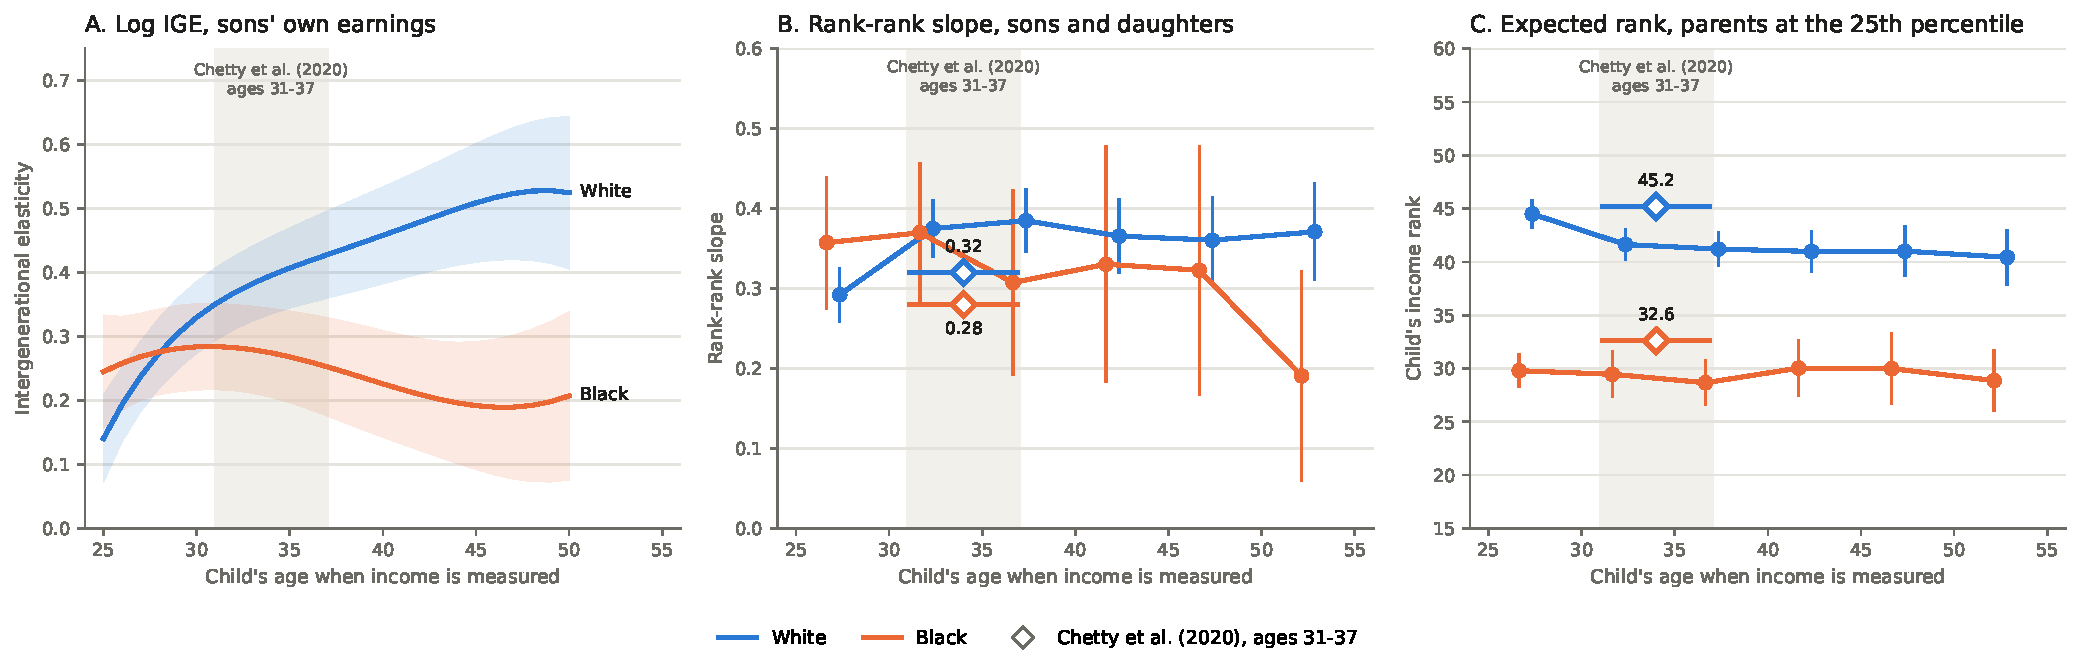
\includegraphics[width=\textwidth]{paperB_age_profile.pdf}
\caption{The age profile of intergenerational persistence, with \citet{chetty2020race} placed on it (PSID)}
\label{fig:headline}
\begin{minipage}{\textwidth}\footnotesize \textit{Notes:} Panel A: log IGE of sons' own earnings at each age, Black
and White, from one Lee--Solon regression with parental income interacted with a quartic in the son's age (child-years
at 25--55; ages above 50 not plotted), 95\% confidence bands. Panel B: rank--rank slope of household income by age band,
sons and daughters, weighted. Panel C: expected household income rank of children whose parents are at the 25th
percentile, by age band. Diamonds: \citet{chetty2020race} at 31--37. Shaded: the 31--37 window. Code:
\texttt{26.IGEByAge.py} (estimates) and \texttt{31.PaperBFigure.py} (figure).\end{minipage}
\end{figure}

\section{What Is Passed On}\label{sec:passedon}

A father's earnings bundle his hourly wage, the hours he works and the years he spends out of work, in a place whose
labor market he shares with other families. Each points to a different policy: schooling and training if the wage is
passed on, tax and transfer incentives or childcare if hours are, unemployment insurance if spells are, place-based
policy if the place is. This section splits the IGE of sons' earnings into these components. The parents' hourly wage
carries a fifth of it, their spells a sixteenth---an eighth at 45--49---hours and place little, and half of the IGE is
parental income at equal values of everything the data measure (Table~\ref{tab:passed_on}).

\subsection{The split}

The split is exact. Write the IGE in an age band as the coefficient $\beta$ of the son's log earnings on log parental
income $\bar y^p$, and the same regression with the parental components $m_k$ added as $\tilde\beta$ and $\gamma_k$.
Then $\beta = \tilde\beta + \sum_k \gamma_k \delta_k$, where $\delta_k$ is the gradient of component $k$ in parental
income \citep{gelbach2016covariates}: a component's contribution is the part of the IGE carried by parental-income
differences that are differences in that component. The components are means over the son's ages 13--19: the father's
and the mother's log hourly wage; their log annual hours and the mother's years without work; the father's shares of
years with a plant closure, a layoff or firing, unemployment and zero hours, the variance of his transitory earnings,
and the mother's share of years unemployed; and the state's unemployment rate and a Bartik shock to men's labor demand
at 12--18. Where a parent is absent or a measure is missing, the measure is set to its mean among the observed and a flag
enters a family-structure row, so that no component is a copy of a flag.\footnote{PSID sons at 25--55 with parental
income over at least three years of their ages 13--19 (4,770 sons, 46,540 son-years), PSID weights, single-age dummies
in every band, standard errors from 200 cluster-bootstrap draws of 1968 families. The father's closures and layoffs are
the PSID's reasons a job ended (plant closed or moved; laid off or fired) in the interview year or the one before. Code:
\texttt{75.WhatIsPassedOn.py} (\texttt{output/what\_is\_passed\_on.md}).} The split is accounting: the components are
correlated choices and outcomes, and Section~\ref{sec:stability} separates the spells the family did not choose.

\begin{table}[!htbp]
\centering
\caption{What is passed on: the earnings IGE split into the parents' components (PSID sons)}
\label{tab:passed_on}
\resizebox{\ifdim\width>\textwidth\textwidth\else\width\fi}{!}{%
\resizebox*{!}{\ifdim\totalheight>0.85\textheight 0.85\textheight\else\totalheight\fi}{%
\begin{tabular}{lcccccc}
\toprule
 & \begin{tabular}[b]{@{}c@{}}25--29\end{tabular} & \begin{tabular}[b]{@{}c@{}}35--39\end{tabular} & \begin{tabular}[b]{@{}c@{}}45--49\end{tabular} & \begin{tabular}[b]{@{}c@{}}25--55\end{tabular} & \begin{tabular}[b]{@{}c@{}}Opening\\45--49 minus\\25--29\end{tabular} & \begin{tabular}[b]{@{}c@{}}Share of\\the IGE,\\25--55 (\%)\end{tabular} \\
 & (1) & (2) & (3) & (4) & (5) & (6) \\
\midrule
\multicolumn{7}{l}{\textit{A. The four components}} \\
IGE & $0.276^{***}$ & $0.430^{***}$ & $0.443^{***}$ & $0.396^{***}$ & $0.167^{***}$ &  \\
 & (0.020) & (0.029) & (0.050) & (0.024) & (0.049) &  \\
Parents' hourly wage & $0.035$ & $0.097^{***}$ & $0.078^{*}$ & $0.075^{***}$ & $0.042$ & $19.0^{***}$ \\
 & (0.022) & (0.027) & (0.041) & (0.022) & (0.038) & (5.3) \\
Parents' hours & $0.013^{**}$ & $0.012^{*}$ & $0.004$ & $0.011^{*}$ & $-0.010$ & $2.8^{**}$ \\
 & (0.006) & (0.007) & (0.012) & (0.006) & (0.011) & (1.3) \\
Parents' spells (stability) & $0.017^{**}$ & $0.019^{*}$ & $0.060^{***}$ & $0.024^{***}$ & $0.043^{**}$ & $6.1^{***}$ \\
 & (0.008) & (0.010) & (0.021) & (0.009) & (0.020) & (2.1) \\
Place (state unemployment, labour demand) & $0.000$ & $0.000$ & $0.005$ & $0.002$ & $0.005$ & $0.4$ \\
 & (0.002) & (0.003) & (0.007) & (0.002) & (0.006) & (0.5) \\
Family structure & $0.035^{**}$ & $0.042^{***}$ & $0.026$ & $0.035^{**}$ & $-0.009$ & $8.8^{***}$ \\
 & (0.015) & (0.015) & (0.029) & (0.014) & (0.028) & (3.2) \\
Rest: parental income at equal components & $0.175^{***}$ & $0.260^{***}$ & $0.271^{***}$ & $0.249^{***}$ & $0.096$ & $62.9^{***}$ \\
 & (0.042) & (0.051) & (0.081) & (0.041) & (0.081) & (8.4) \\
\addlinespace
\multicolumn{7}{l}{\textit{B. With the parents' other resources}} \\
Parents' hourly wage & $0.037$ & $0.049$ & $0.047$ & $0.047^{**}$ & $0.010$ & $12.0^{**}$ \\
 & (0.026) & (0.030) & (0.050) & (0.024) & (0.050) & (5.9) \\
Parents' hours & $0.013^{**}$ & $0.003$ & $-0.009$ & $0.005$ & $-0.021^{*}$ & $1.2$ \\
 & (0.006) & (0.008) & (0.012) & (0.006) & (0.013) & (1.4) \\
Parents' spells (stability) & $0.017^{*}$ & $0.014$ & $0.042^{*}$ & $0.019^{**}$ & $0.025$ & $4.9^{**}$ \\
 & (0.009) & (0.010) & (0.023) & (0.009) & (0.022) & (2.2) \\
Place & $0.001$ & $-0.001$ & $0.004$ & $0.001$ & $0.004$ & $0.2$ \\
 & (0.002) & (0.002) & (0.006) & (0.002) & (0.006) & (0.5) \\
Parents' schooling & $0.008$ & $0.071^{***}$ & $0.065^{***}$ & $0.051^{***}$ & $0.057^{**}$ & $12.9^{***}$ \\
 & (0.013) & (0.017) & (0.024) & (0.014) & (0.024) & (3.7) \\
Transfers (transfer share, AFDC/TANF years) & $0.012$ & $0.026$ & $0.040$ & $0.026^{*}$ & $0.028$ & $6.5^{*}$ \\
 & (0.014) & (0.019) & (0.036) & (0.015) & (0.037) & (3.8) \\
Assets (asset income, home ownership) & $0.021^{*}$ & $-0.011$ & $-0.002$ & $0.001$ & $-0.022$ & $0.1$ \\
 & (0.011) & (0.014) & (0.021) & (0.012) & (0.021) & (2.7) \\
Other members' income & $-0.006$ & $0.003$ & $0.005$ & $0.001$ & $0.012$ & $0.3$ \\
 & (0.005) & (0.005) & (0.008) & (0.004) & (0.009) & (1.1) \\
Family size & $0.003$ & $-0.001$ & $-0.005$ & $0.000$ & $-0.008$ & $0.1$ \\
 & (0.003) & (0.003) & (0.005) & (0.003) & (0.005) & (0.7) \\
Parents' labour income beyond the components & $0.017$ & $0.042$ & $0.071$ & $0.035$ & $0.054$ & $8.9$ \\
 & (0.035) & (0.042) & (0.049) & (0.029) & (0.061) & (7.5) \\
Family structure & $0.027^{*}$ & $0.018$ & $0.016$ & $0.021$ & $-0.011$ & $5.4$ \\
 & (0.016) & (0.022) & (0.033) & (0.017) & (0.032) & (4.5) \\
Rest: parental income at equal measured resources & $0.127^{**}$ & $0.217^{***}$ & $0.169^{*}$ & $0.188^{***}$ & $0.042$ & $47.6^{***}$ \\
 & (0.050) & (0.059) & (0.088) & (0.046) & (0.091) & (10.8) \\
\bottomrule
\end{tabular}}}
\par\smallskip
\begin{minipage}{\textwidth}\footnotesize \textit{Notes:} Contributions to the IGE of sons' ln annual earnings (valid years) on ln parental family income (mean over the son's ages 13--19): exact \citet{gelbach2016covariates} split, each component's contribution = its gradient in parental income times its partial relation to the son's earnings; the rows of a panel sum to the IGE. Components (means over the son's ages 13--19): wage = father's and mother's mean ln hourly wage; hours = their mean ln annual hours, the mother's years without work; spells = the father's shares of years with a plant closure, a layoff or firing, unemployment, zero hours, the variance of his transitory earnings, and the mother's share of years unemployed; place = state unemployment rate and men's Bartik shock at 12--18. Panel B adds the PSID family-file income sources, home ownership, the number of children and the parents' years of schooling. Missing measures are set to the weighted mean of the observed with a flag in the family-structure row. PSID weights; 4,770 sons, 46,540 son-years; standard errors from 200 cluster-bootstrap draws of 1968 families. Source: \texttt{75.WhatIsPassedOn.py}, \texttt{80.WhatIsPassedOnRest.py}; table built by \texttt{90.PaperBRaceNeutralTables.py}. $^{***}$ $p<0.01$, $^{**}$ $p<0.05$, $^{*}$ $p<0.1$.\end{minipage}
\end{table}


\paragraph{The parents' wage.} Over 25--55 the parents' wage carries 0.075$^{***}$ of the IGE of 0.396$^{***}$, a share
of 19.0\%$^{***}$ ($p<0.001$), almost all of it the father's. Its contribution is 0.035 ($p = 0.108$) at 25--29 and
0.097$^{***}$ at 35--39: the wage is passed on, but it shows in the son's earnings only from his mid-thirties.

\paragraph{Hours.} The parents' hours carry 2.8\%$^{**}$ ($p = 0.034$) of the IGE, all of it in the late twenties
(0.013$^{**}$ at 25--29, 0.004 at 45--49).

\paragraph{Spells.} The parents' spells carry 6.1\%$^{***}$ ($p = 0.004$), and they are the one component whose
contribution rises significantly with the son's age: from 0.017$^{**}$ at 25--29 to 0.060$^{***}$ at 45--49, an opening of
0.043$^{**}$ ($p = 0.026$), which is 13.5\%$^{***}$ of the IGE at 45--49. At that age the share is carried by the father's
layoffs (0.025$^{**}$), the mother's unemployment (0.025$^{*}$) and the father's earnings volatility (0.012$^{**}$); the
father's plant closures carry nothing ($-0.001$). Section~\ref{sec:stability} is about this component.

\paragraph{Place.} The state's unemployment rate and labor-demand shocks during the son's teens carry 0.4\% ($p = 0.435$).
Measured by the job finding of men of the family's own race, place carries a tenth of the pooled IGE, entirely between
races (Section~\ref{sec:policy}).

\paragraph{What passes to what.} Table~\ref{tab:four_by_four} shows the partial relations behind the split. Like passes
like. A standard deviation of the father's wage raises the son's wage by 0.083$^{***}$ and the mother's by
0.028$^{**}$; the father's hours raise the son's hours by 0.018$^{***}$ and his employment by 0.009$^{**}$; the mother's
years without work lower the son's employment by 0.021$^{***}$ and raise his share of years unemployed by 0.024$^{***}$.
The father's plant closures, at equal parental income, raise the son's wage (0.021$^{**}$, $p = 0.043$): a closure costs
the family income but, unlike a layoff, says nothing about the father, and the income loss is already in parental
income \citep{gibbons1991layoffs}.

\begin{table}[!htbp]
\centering
\caption{What passes to what: each parental component and each of the son's outcomes (PSID)}
\label{tab:four_by_four}
\resizebox{\ifdim\width>\textwidth\textwidth\else\width\fi}{!}{%
\resizebox*{!}{\ifdim\totalheight>0.85\textheight 0.85\textheight\else\totalheight\fi}{%
\begin{tabular}{lccccc}
\toprule
 & \begin{tabular}[b]{@{}c@{}}Son's ln\\hourly wage\end{tabular} & \begin{tabular}[b]{@{}c@{}}Son's ln hours\\(employed)\end{tabular} & \begin{tabular}[b]{@{}c@{}}Son\\employed\end{tabular} & \begin{tabular}[b]{@{}c@{}}Son's share\\of years\\unemployed\end{tabular} & \begin{tabular}[b]{@{}c@{}}Son's share\\of years\\displaced\end{tabular} \\
 & (1) & (2) & (3) & (4) & (5) \\
\midrule
\multicolumn{6}{l}{\textit{A. Parental income}} \\
Ln parental income & $0.210^{***}$ & $0.038^{**}$ & $0.026^{**}$ & $-0.064^{***}$ & $-0.033^{***}$ \\
 & (0.031) & (0.018) & (0.011) & (0.012) & (0.007) \\
\addlinespace
\multicolumn{6}{l}{\textit{B. Wage}} \\
Father's ln hourly wage & $0.083^{***}$ & $-0.014^{*}$ & $-0.002$ & $0.007$ & $0.009^{**}$ \\
 & (0.016) & (0.008) & (0.005) & (0.005) & (0.004) \\
Mother's ln hourly wage & $0.028^{**}$ & $-0.013^{**}$ & $-0.003$ & $0.006$ & $-0.003$ \\
 & (0.012) & (0.006) & (0.003) & (0.004) & (0.003) \\
\addlinespace
\multicolumn{6}{l}{\textit{C. Hours}} \\
Father's ln annual hours & $0.006$ & $0.018^{***}$ & $0.009^{**}$ & $-0.008^{*}$ & $-0.003$ \\
 & (0.012) & (0.007) & (0.004) & (0.004) & (0.003) \\
Mother's ln annual hours & $-0.039^{***}$ & $0.003$ & $-0.002$ & $0.000$ & $0.000$ \\
 & (0.012) & (0.006) & (0.004) & (0.005) & (0.003) \\
Mother's years without work & $-0.060^{**}$ & $-0.017$ & $-0.021^{***}$ & $0.024^{***}$ & $0.008$ \\
 & (0.024) & (0.011) & (0.008) & (0.009) & (0.005) \\
Mother works fewer than two years & $0.047^{**}$ & $0.008$ & $0.007$ & $-0.019^{**}$ & $-0.009$ \\
 & (0.023) & (0.012) & (0.008) & (0.009) & (0.005) \\
\addlinespace
\multicolumn{6}{l}{\textit{D. Spells}} \\
Father's plant closures & $0.021^{**}$ & $-0.005$ & $0.002$ & $0.001$ & $0.001$ \\
 & (0.010) & (0.006) & (0.003) & (0.004) & (0.002) \\
Father laid off or fired & $-0.013$ & $-0.005$ & $0.004$ & $0.006$ & $0.003$ \\
 & (0.011) & (0.006) & (0.003) & (0.005) & (0.003) \\
Father's unemployment & $-0.018$ & $-0.001$ & $-0.012^{**}$ & $0.011^{*}$ & $0.004$ \\
 & (0.012) & (0.005) & (0.005) & (0.006) & (0.003) \\
Father's zero-hours years & $0.003$ & $-0.001$ & $0.002$ & $0.005$ & $0.005$ \\
 & (0.012) & (0.005) & (0.003) & (0.004) & (0.003) \\
Father's transitory earnings variance & $-0.008$ & $0.006$ & $-0.001$ & $-0.002$ & $-0.001$ \\
 & (0.011) & (0.005) & (0.002) & (0.003) & (0.002) \\
Father present, not measured & $-0.016$ & $-0.010^{*}$ & $-0.007^{**}$ & $0.002$ & $-0.001$ \\
 & (0.011) & (0.005) & (0.004) & (0.005) & (0.003) \\
Mother's unemployment & $-0.020^{*}$ & $-0.010^{**}$ & $-0.009^{*}$ & $0.008^{*}$ & $0.004$ \\
 & (0.011) & (0.005) & (0.005) & (0.005) & (0.003) \\
\addlinespace
\multicolumn{6}{l}{\textit{E. Place}} \\
State unemployment, 12--18 & $-0.007$ & $0.002$ & $0.001$ & $0.006^{*}$ & $0.002$ \\
 & (0.010) & (0.005) & (0.004) & (0.003) & (0.002) \\
Men's labour-demand shock, 12--18 & $0.015$ & $0.008^{*}$ & $0.006^{**}$ & $-0.004$ & $-0.001$ \\
 & (0.010) & (0.004) & (0.003) & (0.003) & (0.002) \\
\bottomrule
\end{tabular}}}
\par\smallskip
\begin{minipage}{\textwidth}\footnotesize \textit{Notes:} Each column is one regression of the son's outcome (son-years 25--55) on ln parental income and every component of Table~\ref{tab:passed_on}, panel A, each standardised (one standard deviation), with the family-structure flags and single-age dummies; PSID weights; standard errors clustered by 1968 family. Columns (1)--(2): 42,225 son-years of 4,644 sons; (3)--(5): 46,540 of 4,770. Source: \texttt{IGE/75.WhatIsPassedOn.py}; table built by \texttt{IGE/90.PaperBRaceNeutralTables.py}. $^{***}$ $p<0.01$, $^{**}$ $p<0.05$, $^{*}$ $p<0.1$.\end{minipage}
\end{table}


\subsection{What is in the rest}

The four components leave 62.9\%$^{***}$ of the IGE as parental income at equal components. Adding the parents' other
resources---their schooling, the family's income from assets, transfers and other members, home ownership, years on
AFDC or TANF and the number of children---brings the rest down to 47.6\%$^{***}$ (panel B).\footnote{PSID family files
1968--2011: head-and-wife taxable and transfer income, AFDC/TANF receipt of the head or wife, own/rent, children in the
family unit; parents' years of schooling. Shares are of family income in the same file. Code:
\texttt{80.WhatIsPassedOnRest.py}.} Two resources carry precise shares. The parents' schooling carries
12.9\%$^{***}$ ($p<0.001$), all of it the father's (0.054$^{***}$; the mother's $-0.003$), and like the wage its
contribution grows with the son's age, from 0.014 at 25--29 to 0.075$^{***}$ at 45--49. Years on AFDC or TANF carry
0.026$^{**}$ ($p = 0.015$), 6.6\% of the IGE. Asset income, home ownership, other members' income and family size carry
nothing. With the father's schooling in, the wage component falls from 19.0\% to 12.0\%$^{**}$: part of what the wage
row measured is the schooling behind it. Half of the IGE remains parental income at equal measured wage, hours, spells,
place, schooling, transfers, assets and family size: money, or what it buys, which these data do not measure
\citep{cardak2013intergenerational, pfeffer2018generations}.

\subsection{Four data sets}

The split replicates where the data measure the components over several years and fails where they are measured once
(Table~\ref{tab:passed_on_data}). In the NLSY79 Children and Young Adults, where the mother is the respondent and her
weekly work history covers every week of the child's teens, the parents' spells carry 7.6\%$^{***}$ ($p = 0.005$) of the
IGE of the children's earnings at 26--35, against 6.0\%$^{**}$ in the PSID at 25--29; there they are the mother's weeks
unemployed and her jobs ending in a firing.\footnote{3,675 children of 2,090 mothers; components over the child's ages
13--17; outcome = mean earnings at 26--35. Code: \texttt{83.CYAWhatIsPassedOn.py}.} In the NLSY79 youths, whose
parents are described once, for the household at 14, the parents' schooling carries 25.0\%$^{***}$ and an occupation-based
wage 1.1\% ($p = 0.35$). In the NLSY97, whose parent interview reports one year of wages and usual hours and the
parents' employment breaks without their reason, wage, hours and breaks carry $-0.5$\%, 0.5\% and $-1.0$\%, while the
parents' schooling and the 1996 transfers carry 22.2\%$^{***}$.\footnote{Code: \texttt{86.NLSY79YouthWhatIsPassedOn.py}
and \texttt{85.NLSY97WhatIsPassedOn.py}.} A component measured in one year does not carry the IGE at equal parental
income, as one year of parental income understates it \citep{solon1992intergenerational, mazumder2005fortunate}; the
parents' schooling, measured once but fixed, carries a fifth to a quarter in both NLS cohorts.

\subsection{By race}

The components differ by race in two places. The spells component opens with age for White sons and not for Black sons
(0.066$^{**}$ against $-0.042$; difference 0.107$^{**}$, $p = 0.018$, on common bootstrap draws), because Black fathers'
layoffs are not concentrated in low-income families (Section~\ref{sec:stability}); and the father's schooling carries
0.065$^{***}$ of the White and 0.002 of the Black IGE. For Black sons family structure carries 60.2\%$^{***}$ of the IGE
and the rest nothing ($-0.008$, $p = 0.92$): the absence of a parent, not parental income at equal parents, is what
the Black IGE transmits.\footnote{Code: \texttt{75.WhatIsPassedOn.py}, \texttt{80.WhatIsPassedOnRest.py},
\texttt{81.StabilityOpeningByRace.py}.}

\section{Why Persistence Rises With Age: Skill at Entry and the Parents' Schooling}\label{sec:skill}

The IGE rises with age because what sons of richer parents bring to the labor market pays more as they age. In the
NLSY79, where the son's tested skill is measured before he enters the labor market, that skill carries three fifths of
the rise of the IGE between 25--29 and 50--54, and the parents' schooling beyond it most of the rest
(Table~\ref{tab:skill_entry}). In the PSID the rise happens within occupations and is predicted by the job a son holds
at 25--34 and by his schooling, whose return rises with age. Everything here is descriptive: skill, schooling and jobs
are outcomes of the same background.

\subsection{Skill at entry}

The NLSY79 follows sons born 1957--64 to their late fifties, and their earnings IGE rises from 0.340$^{***}$ at 25--29 to
0.506$^{***}$ at 50--54, an opening of 0.166$^{***}$ ($p<0.001$). The split of Section~\ref{sec:passedon}, applied to what
the 1979 interview records about the parents---the occupation and work of the adult man and woman at 14, region, the
parents' schooling and reading materials at home---assigns 0.120$^{***}$ ($p<0.001$) of the opening to the parents'
schooling and reading, and nothing to the parents' occupation wage (1.1\%, $p = 0.35$).\footnote{2,952 sons; 1979
weights; 200 cluster-bootstrap draws of 1979 households. Code: \texttt{86.NLSY79YouthWhatIsPassedOn.py}.} The father's
schooling carries the rising part: 0.016 at 25--29, 0.044$^{***}$ at 35--39 and 0.076$^{***}$ at 50--54, the same shape as
in the PSID (0.014 to 0.075$^{***}$ at 45--49; Section~\ref{sec:passedon}).

Adding the son's AFQT, measured in 1980 at ages 15--23, shows how much of that is the son's skill at entry. The AFQT
carries 28.0\%$^{***}$ of the IGE over 25--59, and its contribution rises from 0.077$^{***}$ at 25--29 to 0.181$^{***}$ at
50--54: an opening of 0.103$^{***}$ ($p<0.001$), 62 percent of the opening of the IGE. Seven tenths of the father's
schooling share runs through the son's AFQT (0.027$^{***}$ of 0.039$^{***}$), and two fifths of its rise with age
(0.025$^{***}$ of 0.060$^{***}$). The parents' schooling and reading beyond the AFQT still open by 0.059$^{***}$
($p = 0.004$), and the rest no longer opens (0.003, against 0.048 without the AFQT).\footnote{AFQT-3 (2006 revision),
standardised within birth year over the civilian sample with 1979 weights. Code: \texttt{87.NLSY79YouthAFQT.py}
(\texttt{output/nlsy79\_youth\_afqt.md}).} The AFQT is measured after some of the son's own schooling, so it is his
skill when he enters the labor market, not an endowment.

The rise is age, not the rise of the skill premium in the 1980s and 1990s. The NLSY79 sons reach their late twenties
in 1982--93 and their forties in 1997--2008, when the return to skill was rising nationally. The NLSY97 sons, born
1980--84, reach the same ages twenty years later. In their IGE the AFQT's contribution rises from 0.033$^{***}$ at
25--29 to 0.054$^{***}$ at 40--44 (an opening of 0.021$^{**}$, $p = 0.027$), a factor of 1.64; in the NLSY79 it rises
over the same ages from 0.077$^{***}$ to 0.131$^{***}$, a factor of 1.70 (panel B of Table~\ref{tab:age_period}). In the
hourly wage the NLSY97 contribution opens by 0.029$^{***}$, 43 percent of the opening of the wage IGE.\footnote{The NLSY97
measures parental income in one year, which attenuates the IGE and the AFQT's gradient in parental income alike; the
comparison is of the rise within each cohort. Code: \texttt{94.NLSY97AFQT.py}.}

\begin{table}[!htbp]
\centering
\caption{Why the IGE rises with age: the son's skill at entry and the parents' schooling (NLSY79)}
\label{tab:skill_entry}
\resizebox{\ifdim\width>\textwidth\textwidth\else\width\fi}{!}{%
\resizebox*{!}{\ifdim\totalheight>0.85\textheight 0.85\textheight\else\totalheight\fi}{%
\begin{tabular}{lcccccc}
\toprule
 & \begin{tabular}[b]{@{}c@{}}25--29\end{tabular} & \begin{tabular}[b]{@{}c@{}}35--39\end{tabular} & \begin{tabular}[b]{@{}c@{}}45--49\end{tabular} & \begin{tabular}[b]{@{}c@{}}50--54\end{tabular} & \begin{tabular}[b]{@{}c@{}}25--59\end{tabular} & \begin{tabular}[b]{@{}c@{}}Opening\\50--54 minus\\25--29\end{tabular} \\
 & (1) & (2) & (3) & (4) & (5) & (6) \\
\midrule
\multicolumn{7}{l}{\textit{A. Sons, pooled}} \\
IGE & $0.340^{***}$ & $0.413^{***}$ & $0.486^{***}$ & $0.506^{***}$ & $0.407^{***}$ & $0.166^{***}$ \\
 & (0.022) & (0.027) & (0.035) & (0.042) & (0.022) & (0.037) \\
The son's AFQT & $0.077^{***}$ & $0.123^{***}$ & $0.157^{***}$ & $0.181^{***}$ & $0.114^{***}$ & $0.103^{***}$ \\
 & (0.010) & (0.013) & (0.016) & (0.020) & (0.011) & (0.017) \\
Father's schooling, without the son's AFQT & $0.016$ & $0.044^{***}$ & $0.066^{***}$ & $0.076^{***}$ & $0.039^{***}$ & $0.060^{***}$ \\
 & (0.012) & (0.015) & (0.021) & (0.022) & (0.011) & (0.022) \\
Father's schooling, with the son's AFQT & $-0.002$ & $0.014$ & $0.026$ & $0.033$ & $0.012$ & $0.035^{*}$ \\
 & (0.012) & (0.014) & (0.019) & (0.021) & (0.011) & (0.020) \\
Parents' schooling and reading, without AFQT & $0.050^{***}$ & $0.115^{***}$ & $0.151^{***}$ & $0.170^{***}$ & $0.102^{***}$ & $0.120^{***}$ \\
 & (0.013) & (0.017) & (0.019) & (0.022) & (0.013) & (0.021) \\
Parents' schooling and reading, with AFQT & $0.005$ & $0.037^{**}$ & $0.054^{***}$ & $0.064^{***}$ & $0.033^{**}$ & $0.059^{***}$ \\
 & (0.014) & (0.017) & (0.018) & (0.020) & (0.013) & (0.021) \\
Rest, without AFQT & $0.277^{***}$ & $0.273^{***}$ & $0.295^{***}$ & $0.325^{***}$ & $0.280^{***}$ & $0.048$ \\
 & (0.029) & (0.035) & (0.041) & (0.049) & (0.028) & (0.044) \\
Rest, with AFQT & $0.255^{***}$ & $0.241^{***}$ & $0.243^{***}$ & $0.258^{***}$ & $0.245^{***}$ & $0.003$ \\
 & (0.028) & (0.035) & (0.039) & (0.048) & (0.027) & (0.043) \\
Father's schooling through the son's AFQT & $0.018^{***}$ & $0.029^{***}$ & $0.040^{***}$ & $0.043^{***}$ & $0.027^{***}$ & $0.025^{***}$ \\
 & (0.003) & (0.005) & (0.007) & (0.008) & (0.004) & (0.007) \\
\addlinespace
\multicolumn{7}{l}{\textit{B. White sons}} \\
IGE & $0.292^{***}$ & $0.407^{***}$ & $0.445^{***}$ & $0.480^{***}$ & $0.373^{***}$ & $0.188^{***}$ \\
 & (0.028) & (0.037) & (0.046) & (0.055) & (0.029) & (0.048) \\
The son's AFQT & $0.052^{***}$ & $0.092^{***}$ & $0.115^{***}$ & $0.143^{***}$ & $0.082^{***}$ & $0.091^{***}$ \\
 & (0.010) & (0.014) & (0.018) & (0.022) & (0.012) & (0.018) \\
Father's schooling, without the son's AFQT & $0.015$ & $0.055^{***}$ & $0.080^{***}$ & $0.083^{***}$ & $0.044^{***}$ & $0.067^{**}$ \\
 & (0.015) & (0.019) & (0.027) & (0.029) & (0.015) & (0.028) \\
Father's schooling, with the son's AFQT & $-0.002$ & $0.023$ & $0.035$ & $0.035$ & $0.015$ & $0.038$ \\
 & (0.015) & (0.018) & (0.024) & (0.026) & (0.014) & (0.026) \\
Parents' schooling and reading, without AFQT & $0.035^{**}$ & $0.112^{***}$ & $0.150^{***}$ & $0.172^{***}$ & $0.096^{***}$ & $0.137^{***}$ \\
 & (0.015) & (0.020) & (0.022) & (0.027) & (0.015) & (0.026) \\
Parents' schooling and reading, with AFQT & $-0.003$ & $0.038^{*}$ & $0.052^{**}$ & $0.065^{***}$ & $0.031^{**}$ & $0.068^{***}$ \\
 & (0.016) & (0.020) & (0.022) & (0.024) & (0.015) & (0.024) \\
Rest, without AFQT & $0.247^{***}$ & $0.281^{***}$ & $0.274^{***}$ & $0.311^{***}$ & $0.261^{***}$ & $0.064$ \\
 & (0.035) & (0.044) & (0.050) & (0.060) & (0.034) & (0.053) \\
Rest, with AFQT & $0.239^{***}$ & $0.269^{***}$ & $0.251^{***}$ & $0.273^{***}$ & $0.247^{***}$ & $0.034$ \\
 & (0.034) & (0.042) & (0.047) & (0.058) & (0.033) & (0.053) \\
Father's schooling through the son's AFQT & $0.018^{***}$ & $0.032^{***}$ & $0.045^{***}$ & $0.047^{***}$ & $0.029^{***}$ & $0.030^{***}$ \\
 & (0.004) & (0.006) & (0.009) & (0.010) & (0.005) & (0.009) \\
\bottomrule
\end{tabular}}}
\par\smallskip
\begin{minipage}{\textwidth}\footnotesize \textit{Continued on the next table; notes below its last part.}\end{minipage}
\end{table}
\begin{table}[!htbp]
\centering
\addtocounter{table}{-1}
\caption{Why the IGE rises with age: the son's skill at entry and the parents' schooling (NLSY79) (continued)}
\resizebox{\ifdim\width>\textwidth\textwidth\else\width\fi}{!}{%
\resizebox*{!}{\ifdim\totalheight>0.85\textheight 0.85\textheight\else\totalheight\fi}{%
\begin{tabular}{lcccccc}
\toprule
 & \begin{tabular}[b]{@{}c@{}}25--29\end{tabular} & \begin{tabular}[b]{@{}c@{}}35--39\end{tabular} & \begin{tabular}[b]{@{}c@{}}45--49\end{tabular} & \begin{tabular}[b]{@{}c@{}}50--54\end{tabular} & \begin{tabular}[b]{@{}c@{}}25--59\end{tabular} & \begin{tabular}[b]{@{}c@{}}Opening\\50--54 minus\\25--29\end{tabular} \\
 & (1) & (2) & (3) & (4) & (5) & (6) \\
\midrule
\multicolumn{7}{l}{\textit{C. Black sons}} \\
IGE & $0.298^{***}$ & $0.233^{***}$ & $0.365^{***}$ & $0.362^{***}$ & $0.305^{***}$ & $0.064$ \\
 & (0.034) & (0.040) & (0.058) & (0.056) & (0.031) & (0.060) \\
The son's AFQT & $0.067^{***}$ & $0.087^{***}$ & $0.088^{***}$ & $0.106^{***}$ & $0.080^{***}$ & $0.039^{*}$ \\
 & (0.016) & (0.019) & (0.024) & (0.026) & (0.017) & (0.021) \\
Father's schooling, without the son's AFQT & $0.003$ & $-0.006$ & $0.000$ & $0.027^{*}$ & $0.003$ & $0.023$ \\
 & (0.007) & (0.010) & (0.013) & (0.015) & (0.006) & (0.015) \\
Father's schooling, with the son's AFQT & $-0.002$ & $-0.014$ & $-0.009$ & $0.016$ & $-0.003$ & $0.018$ \\
 & (0.007) & (0.010) & (0.013) & (0.013) & (0.006) & (0.015) \\
Parents' schooling and reading, without AFQT & $0.052^{***}$ & $0.085^{***}$ & $0.118^{***}$ & $0.104^{***}$ & $0.074^{***}$ & $0.052^{*}$ \\
 & (0.017) & (0.021) & (0.030) & (0.033) & (0.017) & (0.030) \\
Parents' schooling and reading, with AFQT & $0.017$ & $0.032$ & $0.065^{**}$ & $0.047$ & $0.030^{*}$ & $0.031$ \\
 & (0.018) & (0.020) & (0.029) & (0.031) & (0.016) & (0.030) \\
Rest, without AFQT & $0.274^{***}$ & $0.131^{***}$ & $0.210^{***}$ & $0.229^{***}$ & $0.225^{***}$ & $-0.044$ \\
 & (0.046) & (0.045) & (0.066) & (0.065) & (0.038) & (0.071) \\
Rest, with AFQT & $0.250^{***}$ & $0.099^{**}$ & $0.184^{***}$ & $0.186^{***}$ & $0.195^{***}$ & $-0.064$ \\
 & (0.045) & (0.046) & (0.066) & (0.063) & (0.036) & (0.070) \\
Father's schooling through the son's AFQT & $0.005^{**}$ & $0.008^{**}$ & $0.009^{**}$ & $0.010^{**}$ & $0.006^{**}$ & $0.005$ \\
 & (0.002) & (0.004) & (0.004) & (0.005) & (0.003) & (0.004) \\
\bottomrule
\end{tabular}}}
\par\smallskip
\begin{minipage}{\textwidth}\footnotesize \textit{Notes:} Contributions to the IGE of sons' ln annual earnings on ln parental income (mean 1978--80) in each age band; exact Gelbach split with the components of Table~\ref{tab:passed_on_data}, column (4), without (A) and with (B) the son's AFQT (AFQT-3, 1980 ASVAB at ages 15--23, standardised within birth year). 'Through the son's AFQT' = the father's-schooling contribution without minus with AFQT, on common bootstrap draws. NLSY79 Black and White youths living with a parent in 1979--81; 1979 weights; 200 cluster-bootstrap draws of 1979 households. Source: \texttt{IGE/86.NLSY79YouthWhatIsPassedOn.py}, \texttt{IGE/87.NLSY79YouthAFQT.py}; table built by \texttt{IGE/90.PaperBRaceNeutralTables.py}. $^{***}$ $p<0.01$, $^{**}$ $p<0.05$, $^{*}$ $p<0.1$.\end{minipage}
\end{table}


The age pattern says why skill at entry pays more later. Under employer learning the return to what employers see at
hiring, schooling, falls with experience while the return to what they learn, ability, rises
\citep{altonji2001employer, lange2007speed}. In the NLSY79 both rise: with the AFQT and schooling in the same
regression, the return to schooling rises by 0.049$^{***}$ from the bands below 35 to the bands above, and the return to
the AFQT by 0.036$^{***}$ (Appendix Table~\ref{tab:afqtgrowth}). Skill and schooling acquired before entry are
complements of the human capital accumulated on the job \citep{bhuller2017life}, and the sons who bring more of them
accumulate faster.

\subsection{Where in the career}

The rise is within occupations. Each son's log wage is split into the CPS wage score of his occupation and his wage
relative to it: the parental-income gradient of the log wage rises from 0.259$^{***}$ at 25--34 to 0.410$^{***}$ at
35--55, and the occupation part barely moves (0.158 to 0.176) while the within-occupation part more than doubles (0.102
to 0.235) (Figure~\ref{fig:career}, Table~\ref{tab:careerdecomp}).\footnote{All PSID occupation codes mapped to the
occ1990dd scheme; the score is the mean log hourly wage of men aged 25--64 in the occupation relative to all men, from
2.9 million CPS Outgoing Rotation Group records of 1979--2019. Code: \texttt{27.CareerWageGrowth.py}.} Background
buys a better-paid occupation at the start, and that advantage hardly grows; what grows is the wage within it.

\begin{figure}[!htbp]
\centering
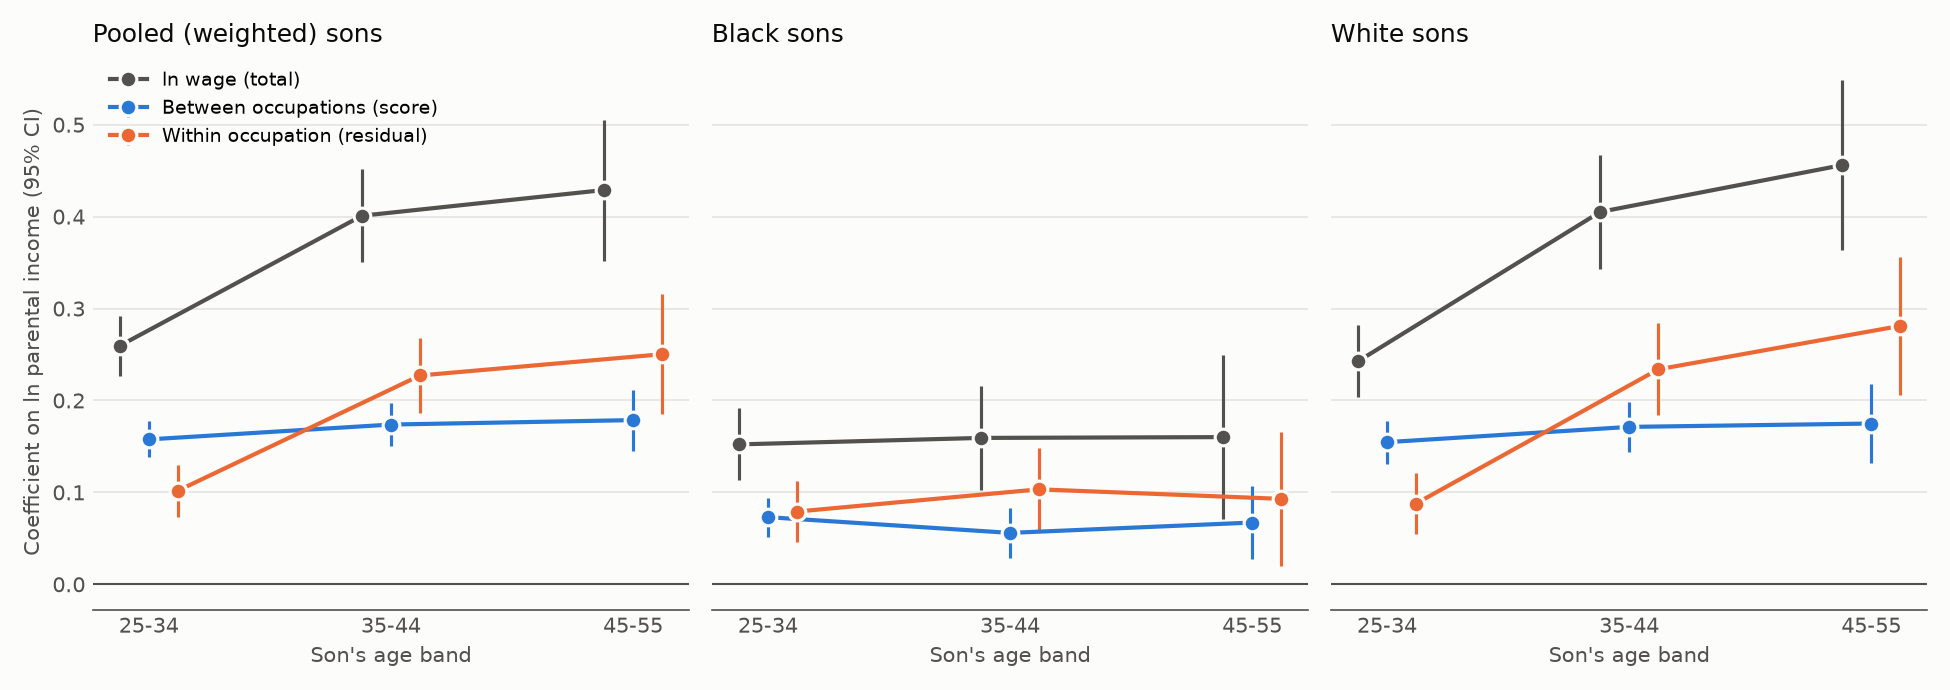
\includegraphics[width=\textwidth]{career_wage_growth.png}
\caption{Wage persistence by the son's age: between and within occupations (PSID)}\label{fig:career}
\begin{minipage}{\textwidth}\footnotesize \textit{Notes:} Coefficient of the son's log wage, of his occupation's wage
score and of his within-occupation residual on log parental income, by age band, with 95\% confidence intervals. The
score and the residual add up to the log wage. Code: \texttt{27.CareerWageGrowth.py}.\end{minipage}
\end{figure}

\begin{table}[!htbp]
\centering
\caption{Wage persistence by age: between and within occupations (PSID, sons)}
\label{tab:careerdecomp}
\resizebox{\ifdim\width>\textwidth\textwidth\else\width\fi}{!}{%
\resizebox*{!}{\ifdim\totalheight>0.85\textheight 0.85\textheight\else\totalheight\fi}{%
\begin{tabular}{lcccc}
\toprule
Panel / row & \begin{tabular}[b]{@{}c@{}}ln wage\end{tabular} & \begin{tabular}[b]{@{}c@{}}Occupation\\score\end{tabular} & \begin{tabular}[b]{@{}c@{}}Within-\\occupation\\residual\end{tabular} & \begin{tabular}[b]{@{}c@{}}Share\\between\\(2)/(1)\end{tabular} \\
 & (1) & (2) & (3) & (4) \\
\midrule
\multicolumn{5}{l}{\textit{Pooled (weighted): coefficient on log parental income}} \\
Sons aged 25--34 & $0.259^{***}$ & $0.158^{***}$ & $0.102^{***}$ & $0.608^{***}$ \\
 & (0.017) & (0.010) & (0.014) & (0.038) \\
Sons aged 35--44 & $0.401^{***}$ & $0.174^{***}$ & $0.227^{***}$ & $0.433^{***}$ \\
 & (0.026) & (0.012) & (0.021) & (0.027) \\
Sons aged 45--55 & $0.429^{***}$ & $0.179^{***}$ & $0.250^{***}$ & $0.416^{***}$ \\
 & (0.039) & (0.017) & (0.033) & (0.037) \\
Sons aged 35--55 & $0.410^{***}$ & $0.176^{***}$ & $0.235^{***}$ & $0.428^{***}$ \\
 & (0.028) & (0.013) & (0.022) & (0.026) \\
Son-years (25--34 / 35--44 / 45--55) & 21,315 / 12,648 / 5,728 &  &  &  \\
\addlinespace
\multicolumn{5}{l}{\textit{Black: coefficient on log parental income}} \\
Sons aged 25--34 & $0.152^{***}$ & $0.073^{***}$ & $0.079^{***}$ & $0.480^{***}$ \\
 & (0.020) & (0.011) & (0.017) & (0.064) \\
Sons aged 35--44 & $0.159^{***}$ & $0.056^{***}$ & $0.103^{***}$ & $0.351^{***}$ \\
 & (0.029) & (0.014) & (0.023) & (0.069) \\
Sons aged 45--55 & $0.160^{***}$ & $0.067^{***}$ & $0.093^{**}$ & $0.420^{***}$ \\
 & (0.046) & (0.020) & (0.037) & (0.111) \\
Sons aged 35--55 & $0.161^{***}$ & $0.060^{***}$ & $0.101^{***}$ & $0.371^{***}$ \\
 & (0.030) & (0.014) & (0.024) & (0.068) \\
Son-years (25--34 / 35--44 / 45--55) & 7,412 / 4,149 / 1,843 &  &  &  \\
\addlinespace
\multicolumn{5}{l}{\textit{White: coefficient on log parental income}} \\
Sons aged 25--34 & $0.243^{***}$ & $0.155^{***}$ & $0.088^{***}$ & $0.638^{***}$ \\
 & (0.020) & (0.012) & (0.017) & (0.049) \\
Sons aged 35--44 & $0.405^{***}$ & $0.171^{***}$ & $0.234^{***}$ & $0.423^{***}$ \\
 & (0.032) & (0.014) & (0.026) & (0.030) \\
Sons aged 45--55 & $0.456^{***}$ & $0.175^{***}$ & $0.281^{***}$ & $0.383^{***}$ \\
 & (0.047) & (0.022) & (0.038) & (0.039) \\
Sons aged 35--55 & $0.418^{***}$ & $0.172^{***}$ & $0.246^{***}$ & $0.411^{***}$ \\
 & (0.033) & (0.015) & (0.026) & (0.028) \\
Son-years (25--34 / 35--44 / 45--55) & 13,915 / 8,500 / 3,885 &  &  &  \\
\addlinespace
\multicolumn{5}{l}{\textit{White $-$ Black: coefficient on log parental income}} \\
Sons aged 25--34 & $0.090^{***}$ & $0.082^{***}$ & $0.009$ & $0.903^{***}$ \\
 & (0.028) & (0.016) & (0.024) & (0.238) \\
Sons aged 35--44 & $0.246^{***}$ & $0.115^{***}$ & $0.131^{***}$ & $0.469^{***}$ \\
 & (0.043) & (0.020) & (0.035) & (0.071) \\
Sons aged 45--55 & $0.296^{***}$ & $0.108^{***}$ & $0.188^{***}$ & $0.364^{***}$ \\
 & (0.066) & (0.030) & (0.053) & (0.083) \\
Sons aged 35--55 & $0.258^{***}$ & $0.112^{***}$ & $0.145^{***}$ & $0.436^{***}$ \\
 & (0.045) & (0.020) & (0.035) & (0.065) \\
\bottomrule
\end{tabular}}}
\par\smallskip
\begin{minipage}{\textwidth}\footnotesize \textit{Continued on the next table; notes below its last part.}\end{minipage}
\end{table}
\begin{table}[!htbp]
\centering
\addtocounter{table}{-1}
\caption{Wage persistence by age: between and within occupations (PSID, sons) (continued)}
\resizebox{\ifdim\width>\textwidth\textwidth\else\width\fi}{!}{%
\resizebox*{!}{\ifdim\totalheight>0.85\textheight 0.85\textheight\else\totalheight\fi}{%
\begin{tabular}{lcccc}
\toprule
Panel / row & \begin{tabular}[b]{@{}c@{}}ln wage\end{tabular} & \begin{tabular}[b]{@{}c@{}}Occupation\\score\end{tabular} & \begin{tabular}[b]{@{}c@{}}Within-\\occupation\\residual\end{tabular} & \begin{tabular}[b]{@{}c@{}}Share\\between\\(2)/(1)\end{tabular} \\
 & (1) & (2) & (3) & (4) \\
\midrule
\multicolumn{5}{l}{\textit{Change in the coefficient across age bands (career divergence)}} \\
Pooled (weighted): (35--55) $-$ (25--34) & $0.151^{***}$ & $0.018^{*}$ & $0.133^{***}$ & $0.119^{*}$ \\
 & (0.023) & (0.010) & (0.021) & (0.062) \\
Pooled (weighted): (45--55) $-$ (25--34) & $0.169^{***}$ & $0.021$ & $0.148^{***}$ & $0.124$ \\
 & (0.035) & (0.015) & (0.032) & (0.081) \\
Black: (35--55) $-$ (25--34) & $0.009$ & $-0.013$ & $0.022$ &  \\
 & (0.025) & (0.011) & (0.022) &  \\
Black: (45--55) $-$ (25--34) & $0.008$ & $-0.006$ & $0.014$ &  \\
 & (0.042) & (0.019) & (0.036) &  \\
White: (35--55) $-$ (25--34) & $0.176^{***}$ & $0.017$ & $0.158^{***}$ & $0.099$ \\
 & (0.027) & (0.012) & (0.024) & (0.063) \\
White: (45--55) $-$ (25--34) & $0.213^{***}$ & $0.020$ & $0.193^{***}$ & $0.095$ \\
 & (0.042) & (0.020) & (0.037) & (0.084) \\
White $-$ Black: (35--55) $-$ (25--34) & $0.167^{***}$ & $0.031^{*}$ & $0.136^{***}$ & $0.184^{**}$ \\
 & (0.037) & (0.016) & (0.032) & (0.087) \\
White $-$ Black: (45--55) $-$ (25--34) & $0.206^{***}$ & $0.026$ & $0.179^{***}$ & $0.127$ \\
 & (0.060) & (0.027) & (0.051) & (0.117) \\
\bottomrule
\end{tabular}}}
\par\smallskip
\begin{minipage}{\textwidth}\footnotesize \textit{Notes:} One regression per cell: the son's outcome (column header) on log parental income (mean at 13--19), son-years in the age band, controls for quartics in the father's age at 16 and the son's age. Occupational wage score: mean log hourly wage of men aged 25--64 in the occupation relative to all men (CPS MORG, base 1992--2002), occupations harmonised to Dorn's occ1990dd scheme; log wage = score (between occupations) + residual (within occupation), so the score and residual columns add up to the log-wage column on the same sample. With a time-varying score (the same relative premium in $t-1$ to $t+1$) the between share of the change of the racial gap is 0.27 (\texttt{output/career\_wage\_growth.md}). Column (4) is left blank when the denominator is not different from zero. All cells are estimated as one stacked system, so differences across bands and groups have standard errors (clustered by 1968 family). Pooled: Black and White sons, weighted; Black and White: unweighted. Sons select into occupations, so the split is accounting, not causal. $^{***}$ $p<0.01$, $^{**}$ $p<0.05$, $^{*}$ $p<0.1$. Source: \texttt{27.CareerWageGrowth.py} (\texttt{output/career\_wage\_growth.csv}); table built by \texttt{28.PaperBTables.py}.\end{minipage}
\end{table}


The job a son holds at 25--34 predicts it. With fixed effects for his modal occupation-by-industry cell at 25--34,
whatever he does later, the parental-income coefficient at 35--55 falls by 0.405$^{***}$ of its rise after 35; his
detailed occupation alone accounts for 0.591$^{***}$ (Table~\ref{tab:earlyjob}).\footnote{93 percent of sons observed
at 35--55 have an early job; randomly reassigning cells gives shares of about 0.03. Code:
\texttt{35.EarlyIndustryLatePayoff.py}.} Access to the jobs whose wages keep growing is unequal by background: 20.2
percent of sons from the top third of parental incomes start in one, 4.7 percent from the bottom third
(Table~\ref{tab:access}). The early job also reflects the son's own skill, so these shares say how far where a son stands
at 25--34 predicts how far he pulls away, not what the job itself does.

\begin{table}[!htbp]
\centering
\caption{Where sons start: the job at 25--34 and the rise of wage persistence after 35 (PSID, sons)}
\label{tab:earlyjob}
\resizebox{\ifdim\width>\textwidth\textwidth\else\width\fi}{!}{%
\resizebox*{!}{\ifdim\totalheight>0.85\textheight 0.85\textheight\else\totalheight\fi}{%
\begin{tabular}{lcccccc}
\toprule
 & \begin{tabular}[b]{@{}c@{}}Accounted\\for at\\25--34\end{tabular} & \begin{tabular}[b]{@{}c@{}}Accounted\\for at\\35--55\end{tabular} & \begin{tabular}[b]{@{}c@{}}Change\end{tabular} & \begin{tabular}[b]{@{}c@{}}Share of\\pooled rise\end{tabular} & \begin{tabular}[b]{@{}c@{}}Change,\\White $-$ Black\end{tabular} & \begin{tabular}[b]{@{}c@{}}Share of\\gap change\end{tabular} \\
 & (1) & (2) & (3) & (4) & (5) & (6) \\
\midrule
\multicolumn{7}{l}{\textit{Fixed effects for the son's job at 25--34, by age band}} \\
Finance, insurance, legal, professional (example; 2 groups) & $0.014^{***}$ & $0.027^{***}$ & $0.013^{**}$ & $0.097^{**}$ & $0.012^{*}$ & $0.085^{*}$ \\
 & (0.003) & (0.007) & (0.005) & (0.039) & (0.006) & (0.046) \\
Industry groups ranked by pay and later growth (4 sets) & $0.024^{***}$ & $0.029^{***}$ & $0.005$ & $0.034$ & $0.001$ & $0.006$ \\
 & (0.005) & (0.008) & (0.005) & (0.037) & (0.008) & (0.058) \\
Industry group (33) & $0.034^{***}$ & $0.052^{***}$ & $0.018^{*}$ & $0.135^{*}$ & $0.015$ & $0.108$ \\
 & (0.007) & (0.013) & (0.010) & (0.072) & (0.016) & (0.105) \\
Manager or professional (2 groups) & $0.042^{***}$ & $0.076^{***}$ & $0.035^{***}$ & $0.257^{***}$ & $0.035^{***}$ & $0.246^{***}$ \\
 & (0.005) & (0.010) & (0.008) & (0.064) & (0.010) & (0.086) \\
Occupation group (11) & $0.057^{***}$ & $0.108^{***}$ & $0.051^{***}$ & $0.377^{***}$ & $0.045^{***}$ & $0.318^{***}$ \\
 & (0.007) & (0.013) & (0.010) & (0.078) & (0.015) & (0.111) \\
Occupation group + industry group (11 + 33) & $0.078^{***}$ & $0.129^{***}$ & $0.050^{***}$ & $0.376^{***}$ & $0.050^{**}$ & $0.352^{***}$ \\
 & (0.010) & (0.017) & (0.012) & (0.087) & (0.020) & (0.129) \\
Cells ranked by pay and later growth (4 sets) & $0.056^{***}$ & $0.093^{***}$ & $0.036^{***}$ & $0.271^{***}$ & $0.033^{***}$ & $0.237^{***}$ \\
 & (0.006) & (0.012) & (0.009) & (0.067) & (0.011) & (0.087) \\
Occupation $\times$ industry cell (11 $\times$ 33) & $0.091^{***}$ & $0.146^{***}$ & $0.054^{***}$ & $0.405^{***}$ & $0.070^{***}$ & $0.493^{***}$ \\
 & (0.011) & (0.020) & (0.015) & (0.099) & (0.025) & (0.171) \\
Detailed occupation (occ1990dd) & $0.086^{***}$ & $0.165^{***}$ & $0.079^{***}$ & $0.591^{***}$ & $0.101^{***}$ & $0.713^{***}$ \\
 & (0.011) & (0.020) & (0.017) & (0.120) & (0.026) & (0.211) \\
\bottomrule
\end{tabular}}}
\par\smallskip
\begin{minipage}{\textwidth}\footnotesize \textit{Notes:} Short regression: the son's log wage on log parental income in each age band (25--34, 35--55), controls as in Table~\ref{tab:industrydecomp}. Long regression: adds fixed effects for the son's job at 25--34 (row), estimated separately in each age band and race sample, so they absorb any wage profile of where he started, linear or not. Accounted for = short $-$ long. On this sample the pooled coefficient rises by 0.132$^{***}$ and the White $-$ Black gap changes by 0.140$^{***}$ from 25--34 to 35--55. Ranked sets: cells (or industries) in the top quartile of men's employment by CPS wage level and by CPS wage growth after 35, and their intersection. Permuting the cell labels across sons gives shares of about 0.03. The son's early job also reflects his own skills, so the rows measure how much where a son stands at 25--34 predicts how far he pulls away, not a causal payoff. 93\% of sons observed at 35--55 have a job at 25--34. Standard errors clustered by 1968 family. $^{***}$ $p<0.01$, $^{**}$ $p<0.05$, $^{*}$ $p<0.1$. Source: \texttt{35.EarlyIndustryLatePayoff.py} (\texttt{output/early\_industry\_late\_payoff.csv}); table built by \texttt{28.PaperBTables.py}.\end{minipage}
\end{table}

\begin{table}[!htbp]
\centering
\caption{Access to well-paid, fast-growing starting jobs at 25--34 (PSID, sons)}
\label{tab:access}
\resizebox{\ifdim\width>\textwidth\textwidth\else\width\fi}{!}{%
\resizebox*{!}{\ifdim\totalheight>0.85\textheight 0.85\textheight\else\totalheight\fi}{%
\begin{tabular}{lccccc}
\toprule
 & \begin{tabular}[b]{@{}c@{}}Well-paid,\\high later\\growth\\(a)\end{tabular} & \begin{tabular}[b]{@{}c@{}}Well-paid,\\high later\\growth\\(b)\end{tabular} & \begin{tabular}[b]{@{}c@{}}Well-paid,\\high later\\growth\\(c)\end{tabular} & \begin{tabular}[b]{@{}c@{}}Well-paid,\\high later\\growth\\(d)\end{tabular} & \begin{tabular}[b]{@{}c@{}}Well-paid,\\high later\\growth\\(e)\end{tabular} \\
 & (1) & (2) & (3) & (4) & (5) \\
\midrule
\multicolumn{6}{l}{\textit{Black and White sons (reference for terciles: Black, bottom tercile)}} \\
ln parental income & $0.104^{***}$ &  & $0.095^{***}$ &  & $0.002$ \\
 & (0.010) &  & (0.011) &  & (0.016) \\
White &  & $0.109^{***}$ & $0.042^{***}$ &  & $0.035^{*}$ \\
 &  & (0.014) & (0.016) &  & (0.020) \\
Black, middle tercile &  &  &  & $0.024$ &  \\
 &  &  &  & (0.022) &  \\
Black, top tercile &  &  &  & $0.125^{***}$ &  \\
 &  &  &  & (0.044) &  \\
White, bottom tercile &  &  &  & $0.048^{**}$ &  \\
 &  &  &  & (0.020) &  \\
White, middle tercile &  &  &  & $0.092^{***}$ &  \\
 &  &  &  & (0.017) &  \\
White, top tercile &  &  &  & $0.187^{***}$ &  \\
 &  &  &  & (0.017) &  \\
Rich White $-$ rich Black (top terciles) &  &  &  & $0.062$ &  \\
 &  &  &  & (0.045) &  \\
Father held a well-paid, high-later-growth job &  &  &  &  & $0.064^{**}$ \\
 &  &  &  &  & (0.025) \\
Years of education &  &  &  &  & $0.063^{***}$ \\
 &  &  &  &  & (0.005) \\
\addlinespace
\multicolumn{6}{l}{\textit{Black sons}} \\
ln parental income & $0.048^{***}$ &  & $0.048^{***}$ &  & $0.021$ \\
 & (0.009) &  & (0.009) &  & (0.018) \\
Middle tercile &  &  &  & $0.022^{*}$ &  \\
 &  &  &  & (0.013) &  \\
Top tercile &  &  &  & $0.104^{***}$ &  \\
 &  &  &  & (0.025) &  \\
Father held a well-paid, high-later-growth job &  &  &  &  & $0.008$ \\
 &  &  &  &  & (0.051) \\
Years of education &  &  &  &  & $0.052^{***}$ \\
 &  &  &  &  & (0.007) \\
\addlinespace
\multicolumn{6}{l}{\textit{White sons}} \\
ln parental income & $0.103^{***}$ &  & $0.103^{***}$ &  & $-0.001$ \\
 & (0.012) &  & (0.012) &  & (0.016) \\
Middle tercile &  &  &  & $0.050^{***}$ &  \\
 &  &  &  & (0.018) &  \\
Top tercile &  &  &  & $0.138^{***}$ &  \\
 &  &  &  & (0.019) &  \\
Father held a well-paid, high-later-growth job &  &  &  &  & $0.048^{**}$ \\
 &  &  &  &  & (0.023) \\
Years of education &  &  &  &  & $0.064^{***}$ \\
 &  &  &  &  & (0.005) \\
\bottomrule
\end{tabular}}}
\par\smallskip
\begin{minipage}{\textwidth}\footnotesize \textit{Continued on the next table; notes below its last part.}\end{minipage}
\end{table}
\begin{table}[!htbp]
\centering
\addtocounter{table}{-1}
\caption{Access to well-paid, fast-growing starting jobs at 25--34 (PSID, sons) (continued)}
\resizebox{\ifdim\width>\textwidth\textwidth\else\width\fi}{!}{%
\resizebox*{!}{\ifdim\totalheight>0.85\textheight 0.85\textheight\else\totalheight\fi}{%
\begin{tabular}{lccccc}
\toprule
 & \begin{tabular}[b]{@{}c@{}}Well-paid,\\high later\\growth\\(a)\end{tabular} & \begin{tabular}[b]{@{}c@{}}Well-paid,\\high later\\growth\\(b)\end{tabular} & \begin{tabular}[b]{@{}c@{}}Well-paid,\\high later\\growth\\(c)\end{tabular} & \begin{tabular}[b]{@{}c@{}}Well-paid,\\high later\\growth\\(d)\end{tabular} & \begin{tabular}[b]{@{}c@{}}Well-paid,\\high later\\growth\\(e)\end{tabular} \\
 & (1) & (2) & (3) & (4) & (5) \\
\midrule
\multicolumn{6}{l}{\textit{White $-$ Black}} \\
ln parental income & $0.055^{***}$ &  & $0.055^{***}$ &  & $-0.022$ \\
 & (0.015) &  & (0.015) &  & (0.024) \\
Middle tercile &  &  &  & $0.028$ &  \\
 &  &  &  & (0.022) &  \\
Top tercile &  &  &  & $0.034$ &  \\
 &  &  &  & (0.031) &  \\
Father held a well-paid, high-later-growth job &  &  &  &  & $0.040$ \\
 &  &  &  &  & (0.056) \\
Years of education &  &  &  &  & $0.012$ \\
 &  &  &  &  & (0.008) \\
\bottomrule
\end{tabular}}}
\par\smallskip
\begin{minipage}{\textwidth}\footnotesize \textit{Notes:} Son-level linear probability models. Outcome in columns (1)--(5): the son's job at 25--34 (modal occupation $\times$ industry cell) is in the top quartile of men's employment by both CPS wage level and CPS wage growth after 35 (mean 0.156); the same specifications for well-paid jobs of any kind are in \texttt{output/early\_industry\_late\_payoff.md}, Section D3. Specifications (a) log parental income; (b) White; (c) both; (d) race $\times$ parental-income tercile; (e) (c) plus the father's job and the son's years of education. Pooled: weighted; by race: unweighted. Standard errors clustered by 1968 family. $^{***}$ $p<0.01$, $^{**}$ $p<0.05$, $^{*}$ $p<0.1$. Source: \texttt{IGE/35.EarlyIndustryLatePayoff.py} (\texttt{output/early\_industry\_late\_payoff.csv}); table built by \texttt{IGE/28.PaperBTables.py}.\end{minipage}
\end{table}


Schooling carries much of it. Adding the son's years of schooling to the regression of his log wage on parental income
by band removes 0.057$^{***}$ of the rise of wage persistence after 35, a share of 0.44$^{***}$; for earnings 0.090$^{***}$
of 0.203$^{***}$ (0.44$^{***}$), and in the NLSY79 0.038$^{***}$ of 0.054$^{**}$ (0.72$^{**}$).\footnote{Code:
\texttt{42.SchoolingAndJobGrowth.py}.} The return to a year of schooling rises with age, and half of its rise is the
sorting of the educated into jobs whose wages grow: holding the early job fixed halves the rise of the earnings return,
from 0.050$^{***}$ to 0.025$^{***}$ (Table~\ref{tab:withincell}).

\subsection{By race}

The rise of the IGE with age is a White phenomenon (Section~\ref{sec:ageprofile}), and so are its carriers. The AFQT's
contribution opens by 0.091$^{***}$ for White sons and by 0.039$^{*}$ ($p = 0.069$) for Black sons, and the father's
schooling carries nothing for Black sons in either data set (Table~\ref{tab:skill_entry}, panels B and C). The return to
schooling rises with age faster for White than for Black sons---a difference of 0.058$^{***}$ in the rise of the earnings
return, 0.061$^{***}$ within the son's cell at 25--34, 0.063$^{**}$ net of a calendar trend in the return, and in the
NLSY79 0.021$^{**}$ at equal AFQT (Tables~\ref{tab:schooling} and \ref{tab:withincell})---while the AFQT return rises
equally ($-0.031$, s.e.\ 0.025) and, as \citet{rauh2023black} find, wages grow with experience at the same rate at equal
AFQT.\footnote{Black $\times$ experience 0.003 in logs (s.e.\ 0.003) in their within-decile regression with the NLSY79
supplemental Black sample; code \texttt{70.RauhReplication.py}.} At equal parental income White sons are 4.2
percentage points more likely to start in the jobs whose wages keep growing (0.042$^{***}$), and with the same employer a
White son's wage grows faster with parental income (0.021$^{***}$ a year per log point at 25--34) while a Black son's
does not (0.003) (Table~\ref{tab:growthladder}).\footnote{Code: \texttt{35.EarlyIndustryLatePayoff.py},
\texttt{36.SameEmployerGrowthChecks.py}, \texttt{45.WithinCellIdentification.py}.}

\begin{table}[!htbp]
\centering
\caption{The return to schooling by age and race, and the part of wage persistence it carries}
\label{tab:schooling}
\resizebox{\ifdim\width>\textwidth\textwidth\else\width\fi}{!}{%
\resizebox*{!}{\ifdim\totalheight>0.85\textheight 0.85\textheight\else\totalheight\fi}{%
\begin{tabular}{lccccccc}
\toprule
 & \begin{tabular}[b]{@{}c@{}}PSID\\ln hourly wage\\on education\end{tabular} & \begin{tabular}[b]{@{}c@{}}PSID\\ln earnings\\on education\end{tabular} & \begin{tabular}[b]{@{}c@{}}NLSY79\\ln hourly wage\\on education\end{tabular} & \begin{tabular}[b]{@{}c@{}}PSID\\ln hourly wage\\on ln parental\\income\end{tabular} & \begin{tabular}[b]{@{}c@{}}PSID\\accounted for\\by education\end{tabular} & \begin{tabular}[b]{@{}c@{}}NLSY79\\ln hourly wage\\on ln parental\\income\end{tabular} & \begin{tabular}[b]{@{}c@{}}NLSY79\\accounted for\\by education\end{tabular} \\
 & (1) & (2) & (3) & (4) & (5) & (6) & (7) \\
\midrule
\multicolumn{8}{l}{\textit{White sons}} \\
Age 25--29 & $0.049^{***}$ & $0.045^{***}$ & $0.046^{***}$ & $0.220^{***}$ & $0.046^{***}$ & $0.222^{***}$ & $0.048^{***}$ \\
 & (0.005) & (0.007) & (0.004) & (0.018) & (0.008) & (0.018) & (0.007) \\
Age 30--34 & $0.090^{***}$ & $0.101^{***}$ & $0.072^{***}$ & $0.342^{***}$ & $0.101^{***}$ & $0.263^{***}$ & $0.082^{***}$ \\
 & (0.006) & (0.007) & (0.005) & (0.024) & (0.011) & (0.023) & (0.009) \\
Age 35--39 & $0.110^{***}$ & $0.122^{***}$ & $0.097^{***}$ & $0.384^{***}$ & $0.128^{***}$ & $0.319^{***}$ & $0.116^{***}$ \\
 & (0.007) & (0.008) & (0.005) & (0.030) & (0.014) & (0.025) & (0.012) \\
Age 40--44 & $0.128^{***}$ & $0.143^{***}$ & $0.120^{***}$ & $0.440^{***}$ & $0.153^{***}$ & $0.338^{***}$ & $0.149^{***}$ \\
 & (0.008) & (0.009) & (0.005) & (0.037) & (0.017) & (0.028) & (0.014) \\
Age 45--49 & $0.125^{***}$ & $0.130^{***}$ & $0.122^{***}$ & $0.465^{***}$ & $0.140^{***}$ & $0.348^{***}$ & $0.153^{***}$ \\
 & (0.010) & (0.011) & (0.006) & (0.050) & (0.020) & (0.031) & (0.015) \\
Age 50--55 & $0.128^{***}$ & $0.128^{***}$ & $0.123^{***}$ & $0.455^{***}$ & $0.162^{***}$ & $0.367^{***}$ & $0.146^{***}$ \\
 & (0.012) & (0.014) & (0.007) & (0.053) & (0.026) & (0.035) & (0.016) \\
\textbf{Change, 35+ minus below 35} & $0.053^{***}$ & $0.057^{***}$ & $0.056^{***}$ & $0.155^{***}$ & $0.072^{***}$ & $0.100^{***}$ & $0.076^{***}$ \\
 & (0.007) & (0.008) & (0.004) & (0.030) & (0.013) & (0.020) & (0.009) \\
\addlinespace
\multicolumn{8}{l}{\textit{Black sons}} \\
Age 25--29 & $0.076^{***}$ & $0.124^{***}$ & $0.068^{***}$ & $0.174^{***}$ & $0.037^{***}$ & $0.146^{***}$ & $0.047^{***}$ \\
 & (0.007) & (0.010) & (0.006) & (0.020) & (0.007) & (0.018) & (0.007) \\
Age 30--34 & $0.101^{***}$ & $0.151^{***}$ & $0.086^{***}$ & $0.199^{***}$ & $0.058^{***}$ & $0.178^{***}$ & $0.060^{***}$ \\
 & (0.008) & (0.010) & (0.008) & (0.023) & (0.010) & (0.020) & (0.010) \\
Age 35--39 & $0.106^{***}$ & $0.144^{***}$ & $0.105^{***}$ & $0.187^{***}$ & $0.062^{***}$ & $0.165^{***}$ & $0.074^{***}$ \\
 & (0.009) & (0.012) & (0.008) & (0.030) & (0.010) & (0.025) & (0.013) \\
Age 40--44 & $0.096^{***}$ & $0.127^{***}$ & $0.115^{***}$ & $0.140^{***}$ & $0.042^{***}$ & $0.225^{***}$ & $0.090^{***}$ \\
 & (0.011) & (0.014) & (0.010) & (0.034) & (0.011) & (0.027) & (0.016) \\
Age 45--49 & $0.118^{***}$ & $0.146^{***}$ & $0.127^{***}$ & $0.145^{***}$ & $0.057^{***}$ & $0.206^{***}$ & $0.095^{***}$ \\
 & (0.012) & (0.016) & (0.010) & (0.042) & (0.016) & (0.029) & (0.017) \\
Age 50--55 & $0.121^{***}$ & $0.143^{***}$ & $0.132^{***}$ & $0.150^{***}$ & $0.040^{**}$ & $0.238^{***}$ & $0.105^{***}$ \\
 & (0.016) & (0.021) & (0.010) & (0.057) & (0.019) & (0.032) & (0.017) \\
\textbf{Change, 35+ minus below 35} & $0.021^{**}$ & $0.002$ & $0.043^{***}$ & $-0.030$ & $0.003$ & $0.047^{***}$ & $0.038^{***}$ \\
 & (0.009) & (0.011) & (0.006) & (0.029) & (0.009) & (0.018) & (0.009) \\
\addlinespace
\multicolumn{8}{l}{\textit{White $-$ Black}} \\
Age 25--29 & $-0.027^{***}$ & $-0.079^{***}$ & $-0.022^{***}$ & $0.046^{*}$ & $0.009$ & $0.076^{***}$ & $0.000$ \\
 & (0.009) & (0.012) & (0.007) & (0.027) & (0.011) & (0.026) & (0.010) \\
Age 30--34 & $-0.011$ & $-0.049^{***}$ & $-0.013$ & $0.143^{***}$ & $0.043^{***}$ & $0.085^{***}$ & $0.023^{*}$ \\
 & (0.010) & (0.013) & (0.009) & (0.033) & (0.015) & (0.030) & (0.013) \\
Age 35--39 & $0.005$ & $-0.022$ & $-0.008$ & $0.197^{***}$ & $0.065^{***}$ & $0.154^{***}$ & $0.041^{**}$ \\
 & (0.012) & (0.015) & (0.010) & (0.043) & (0.017) & (0.035) & (0.017) \\
Age 40--44 & $0.032^{**}$ & $0.016$ & $0.004$ & $0.299^{***}$ & $0.111^{***}$ & $0.113^{***}$ & $0.060^{***}$ \\
 & (0.014) & (0.017) & (0.012) & (0.051) & (0.020) & (0.039) & (0.021) \\
Age 45--49 & $0.007$ & $-0.015$ & $-0.004$ & $0.320^{***}$ & $0.083^{***}$ & $0.142^{***}$ & $0.059^{***}$ \\
 & (0.016) & (0.020) & (0.011) & (0.066) & (0.025) & (0.043) & (0.022) \\
Age 50--55 & $0.008$ & $-0.015$ & $-0.009$ & $0.305^{***}$ & $0.122^{***}$ & $0.129^{***}$ & $0.041^{*}$ \\
 & (0.020) & (0.025) & (0.013) & (0.078) & (0.032) & (0.047) & (0.024) \\
\textbf{Change, 35+ minus below 35} & $0.032^{***}$ & $0.055^{***}$ & $0.013^{*}$ & $0.186^{***}$ & $0.069^{***}$ & $0.054^{**}$ & $0.038^{***}$ \\
 & (0.011) & (0.014) & (0.008) & (0.041) & (0.016) & (0.027) & (0.013) \\
\bottomrule
\end{tabular}}}
\par\smallskip
\begin{minipage}{\textwidth}\footnotesize \textit{Notes:} Son-years at 25--55 with a valid wage, years of education and parental income; one regression per column and age band, controls: quartic in age and year (round) fixed effects. Columns (1)--(3): coefficient on years of completed education. Columns (4) and (6): coefficient on log parental income. Columns (5) and (7): the part of (4) and (6) that disappears when years of education are added (the return to education times the education gradient in parental income). Change row: mean over the bands from 35 minus mean over the bands below 35. White $-$ Black: difference of the separate regressions, standard errors from joint influence functions, clustered by 1968 family (PSID) or 1979 household (NLSY79). $^{***}$ $p<0.01$, $^{**}$ $p<0.05$, $^{*}$ $p<0.1$. Source: \texttt{42.SchoolingAndJobGrowth.py} (\texttt{output/schooling\_job\_growth.csv}).\end{minipage}
\end{table}

\begin{table}[!htbp]
\centering
\caption{Does the racial difference in the pay-off of schooling survive within jobs?}
\label{tab:withincell}
\resizebox{\ifdim\width>\textwidth\textwidth\else\width\fi}{!}{%
\resizebox*{!}{\ifdim\totalheight>0.85\textheight 0.85\textheight\else\totalheight\fi}{%
\begin{tabular}{lccccc}
\toprule
 & \begin{tabular}[b]{@{}c@{}}Baseline\end{tabular} & \begin{tabular}[b]{@{}c@{}}Early-cell\\fixed effects\end{tabular} & \begin{tabular}[b]{@{}c@{}}Current-cell\\fixed effects\end{tabular} & \begin{tabular}[b]{@{}c@{}}Schooling $\times$\\calendar trend\end{tabular} & \begin{tabular}[b]{@{}c@{}}Born\\1955--69\end{tabular} \\
 & (1) & (2) & (3) & (4) & (5) \\
\midrule
\multicolumn{6}{l}{\textit{PSID, log annual earnings}} \\
White: rise of the return, 35+ minus below 35 & $0.057^{***}$ & $0.035^{***}$ & $0.032^{***}$ & $0.041^{***}$ & $0.064^{***}$ \\
 & (0.008) & (0.010) & (0.009) & (0.015) & (0.010) \\
Black: rise of the return, 35+ minus below 35 & $-0.001$ & $-0.025^{*}$ & $-0.034^{***}$ & $-0.022$ & $0.013$ \\
 & (0.012) & (0.015) & (0.013) & (0.023) & (0.016) \\
White $-$ Black: rise of the return & $0.058^{***}$ & $0.061^{***}$ & $0.066^{***}$ & $0.063^{**}$ & $0.051^{***}$ \\
 & (0.014) & (0.018) & (0.016) & (0.027) & (0.019) \\
White $-$ Black: return at 25--29 & $-0.077^{***}$ & $-0.061^{***}$ & $-0.066^{***}$ & $-0.079^{***}$ & $-0.057^{***}$ \\
 & (0.012) & (0.015) & (0.012) & (0.012) & (0.019) \\
\addlinespace
\multicolumn{6}{l}{\textit{PSID, log hourly wage}} \\
White: rise of the return, 35+ minus below 35 & $0.052^{***}$ & $0.032^{***}$ & $0.028^{***}$ & $0.038^{***}$ & $0.060^{***}$ \\
 & (0.007) & (0.009) & (0.008) & (0.014) & (0.009) \\
Black: rise of the return, 35+ minus below 35 & $0.021^{**}$ & $0.003$ & $-0.008$ & $0.003$ & $0.031^{**}$ \\
 & (0.009) & (0.012) & (0.010) & (0.018) & (0.013) \\
White $-$ Black: rise of the return & $0.031^{***}$ & $0.029^{*}$ & $0.036^{***}$ & $0.035$ & $0.029^{*}$ \\
 & (0.011) & (0.015) & (0.013) & (0.023) & (0.016) \\
White $-$ Black: return at 25--29 & $-0.028^{***}$ & $-0.023^{**}$ & $-0.030^{***}$ & $-0.028^{***}$ & $-0.016$ \\
 & (0.009) & (0.010) & (0.009) & (0.009) & (0.014) \\
\addlinespace
\multicolumn{6}{l}{\textit{NLSY79, log hourly rate of pay}} \\
White: rise of the return, 35+ minus below 35 & $0.056^{***}$ & $0.044^{***}$ & $0.046^{***}$ &  &  \\
 & (0.004) & (0.006) & (0.005) &  &  \\
Black: rise of the return, 35+ minus below 35 & $0.044^{***}$ & $0.027^{***}$ & $0.029^{***}$ &  &  \\
 & (0.006) & (0.009) & (0.007) &  &  \\
White $-$ Black: rise of the return & $0.012$ & $0.017$ & $0.017^{*}$ &  &  \\
 & (0.008) & (0.010) & (0.009) &  &  \\
White $-$ Black: return at 25--29 & $-0.022^{***}$ & $-0.008$ & $-0.004$ &  &  \\
 & (0.007) & (0.008) & (0.007) &  &  \\
\bottomrule
\end{tabular}}}
\par\smallskip
\begin{minipage}{\textwidth}\footnotesize \textit{Notes:} Coefficient on years of schooling in a regression of the log outcome by age band (25--29 to 50--55) and race; rows give its rise (mean over the bands from 35 minus mean below 35) and, for the race difference, its value at 25--29. Controls: quartic in age, year (round) fixed effects. Early cell: the son's modal occupation group $\times$ industry group (11 $\times$ 33) at 25--34; current cell: the same at each observation. Column (4) adds schooling $\times$ (year $-$ 1995)/10, so the return is evaluated in 1995 and the rise is net of the calendar trend of the return; column (5) keeps sons born 1955--69. The NLSY79 is one cohort, so (4)--(5) are not defined there. All columns use the same son-years (early cell known). Standard errors clustered by 1968 family (PSID) or 1979 household (NLSY79). $^{***}$ $p<0.01$, $^{**}$ $p<0.05$, $^{*}$ $p<0.1$. Source: \texttt{45.WithinCellIdentification.py} (\texttt{output/within\_cell\_identification.csv}).\end{minipage}
\end{table}


\section{Spells in Childhood: Why Stability Is Passed On More With Age}\label{sec:stability}

The parents' spells are the one component of Section~\ref{sec:passedon} whose share rises with the son's age, and the
reason is that a father's layoff in his son's teens costs the son more the older the son gets. At equal parental income
and equal values of every other component, a layoff is unrelated to the son's earnings at 25--29 and lowers them by
0.110$^{***}$ log points a layoff year at 45--49; a plant closure does neither. The cost is in the son's wage, it grows
within the same son, and only layoffs during his teens carry it. The same contrast shows in which parental income is
passed on: income tied to layoffs and unemployment passes on twice as strongly as other income, income lost to plant
closures no more strongly. The son's own spells run the other way: they carry three tenths of the IGE at 25--29 and a
tenth at 45--49. Everything in this section is descriptive; a layoff is not assigned at random, and the closure is the
comparison that comes closest to a shock the family did not choose.

\subsection{A layoff in the teens costs the son more as he ages}

Table~\ref{tab:layoff_age} reports the partial coefficient behind the spells component: the coefficient of the
father's share of the son's ages 13--19 with a layoff or firing on the son's log earnings in each age band, holding log
parental income and every component of Table~\ref{tab:passed_on} fixed. It is 0.146 ($p = 0.19$) at 25--29, falls in
every band, and reaches $-0.768^{***}$ ($p = 0.005$) at 45--49; the change between the two bands is $-0.914^{***}$
($p<0.001$). The share is over seven years, so one layoff year lowers the son's earnings at 45--49 by 0.110 log points.
Five-year birth-cohort dummies leave the profile unchanged ($-0.739^{***}$ at 45--49, change $-0.866^{***}$), so it is
not that later-born sons are observed only young. The father's plant closures show no profile: 0.127 at 25--29, 0.127
at 45--49, a change of 0.000 (s.e.\ 0.258).\footnote{Father present; the mean layoff share is 0.044 and 12 percent of
sons have a layoff year. Layoff = the PSID's reason a job ended `laid off or fired', closure = `plant closed or moved',
in the interview year or the one before. Code: \texttt{88.LayoffCostByAge.py} (\texttt{output/layoff\_cost\_by\_age.md}).}

\begin{table}[!htbp]
\centering
\caption{A childhood layoff costs the son more as he ages (PSID)}
\label{tab:layoff_age}
\resizebox{\ifdim\width>\textwidth\textwidth\else\width\fi}{!}{%
\resizebox*{!}{\ifdim\totalheight>0.85\textheight 0.85\textheight\else\totalheight\fi}{%
\begin{tabular}{lccccccc}
\toprule
 & \begin{tabular}[b]{@{}c@{}}25--29\end{tabular} & \begin{tabular}[b]{@{}c@{}}30--34\end{tabular} & \begin{tabular}[b]{@{}c@{}}35--39\end{tabular} & \begin{tabular}[b]{@{}c@{}}40--44\end{tabular} & \begin{tabular}[b]{@{}c@{}}45--49\end{tabular} & \begin{tabular}[b]{@{}c@{}}50--55\end{tabular} & \begin{tabular}[b]{@{}c@{}}Change\\45--49 minus\\25--29\end{tabular} \\
 & (1) & (2) & (3) & (4) & (5) & (6) & (7) \\
\midrule
\multicolumn{8}{l}{\textit{A. Ln earnings, single-age dummies}} \\
Father laid off or fired, all sons & $0.146$ & $-0.006$ & $-0.110$ & $-0.241$ & $-0.768^{***}$ & $-0.543$ & $-0.914^{***}$ \\
 & (0.111) & (0.135) & (0.157) & (0.216) & (0.272) & (0.369) & (0.252) \\
Father's plant closed, all sons & $0.127$ & $0.143$ & $0.415^{**}$ & $0.229$ & $0.127$ & $-0.018$ & $0.000$ \\
 & (0.144) & (0.199) & (0.188) & (0.260) & (0.295) & (0.397) & (0.258) \\
Father laid off or fired, White sons & $0.158$ & $-0.033$ & $-0.097$ & $-0.267$ & $-0.818^{***}$ & $-0.621$ & $-0.975^{***}$ \\
 & (0.118) & (0.149) & (0.174) & (0.232) & (0.297) & (0.442) & (0.274) \\
Father laid off or fired, Black sons & $-0.218$ & $-0.064$ & $-0.379$ & $-0.107$ & $-0.351$ & $-0.133$ & $-0.133$ \\
 & (0.279) & (0.341) & (0.453) & (0.473) & (0.444) & (0.321) & (0.431) \\
\addlinespace
\multicolumn{8}{l}{\textit{B. Ln earnings, with five-year birth-cohort dummies}} \\
Father laid off or fired, all sons & $0.127$ & $-0.013$ & $-0.116$ & $-0.245$ & $-0.739^{***}$ & $-0.543$ & $-0.866^{***}$ \\
 & (0.108) & (0.140) & (0.159) & (0.218) & (0.260) & (0.351) & (0.242) \\
Father's plant closed, all sons & $0.106$ & $0.121$ & $0.412^{**}$ & $0.220$ & $0.086$ & $-0.038$ & $-0.020$ \\
 & (0.146) & (0.200) & (0.189) & (0.259) & (0.286) & (0.394) & (0.253) \\
Father laid off or fired, White sons & $0.152$ & $-0.037$ & $-0.097$ & $-0.273$ & $-0.774^{***}$ & $-0.614$ & $-0.926^{***}$ \\
 & (0.118) & (0.154) & (0.175) & (0.235) & (0.284) & (0.419) & (0.263) \\
Father laid off or fired, Black sons & $-0.334$ & $-0.037$ & $-0.383$ & $-0.096$ & $-0.408$ & $-0.094$ & $-0.075$ \\
 & (0.286) & (0.342) & (0.451) & (0.426) & (0.437) & (0.343) & (0.441) \\
\addlinespace
\multicolumn{8}{l}{\textit{C. Which outcome: father laid off or fired (columns 25--29, 45--49 and the change)}} \\
All sons: ln annual earnings & $0.146$ &  &  &  & $-0.768^{***}$ &  & $-0.914^{***}$ \\
 & (0.111) &  &  &  & (0.272) &  & (0.252) \\
All sons: ln hourly wage & $0.046$ &  &  &  & $-0.557^{***}$ &  & $-0.603^{***}$ \\
 & (0.089) &  &  &  & (0.213) &  & (0.203) \\
All sons: ln annual hours (employed) & $0.100^{*}$ &  &  &  & $-0.211$ &  & $-0.311^{**}$ \\
 & (0.059) &  &  &  & (0.143) &  & (0.139) \\
All sons: employed & $0.050^{*}$ &  &  &  & $0.083$ &  & $0.033$ \\
 & (0.026) &  &  &  & (0.078) &  & (0.080) \\
All sons: his share of years unemployed & $0.008$ &  &  &  & $0.030$ &  & $0.022$ \\
 & (0.075) &  &  &  & (0.086) &  & (0.103) \\
\bottomrule
\end{tabular}}}
\par\smallskip
\begin{minipage}{\textwidth}\footnotesize \textit{Notes:} Coefficient of the father's share of the son's ages 13--19 with a layoff or firing (PSID 'laid off / fired') or a plant closure ('plant closed / moved') on the son's outcome in each age band, holding ln parental income and every component of Table~\ref{tab:passed_on}, panel A, fixed; single-age dummies; PSID weights. The share is over seven years, so one year with a layoff is one seventh of the coefficient. Father present; mean layoff share 0.044, 12 percent of sons have a layoff year. Standard errors from 200 cluster-bootstrap draws of 1968 families. Source: \texttt{88.LayoffCostByAge.py}; table built by \texttt{90.PaperBRaceNeutralTables.py}. $^{***}$ $p<0.01$, $^{**}$ $p<0.05$, $^{*}$ $p<0.1$.\end{minipage}
\end{table}


The cost is in the wage. In panel C the coefficient on the son's log hourly wage changes by $-0.603^{***}$ ($p = 0.003$)
between 25--29 and 45--49, two thirds of the change in earnings, and that on his annual hours when employed by
$-0.311^{**}$ ($p = 0.025$); his employment ($0.033$) and his share of years unemployed ($0.022$) do not change. A son
whose father was laid off in his teens works as much as other sons at 45--49 and is paid less per hour.

\paragraph{Within the same son.} The profile across bands compares different sons at different ages. Table~\ref{tab:layoff_fe}
follows the same son: with son fixed effects, the father's layoff share interacted with the son's age measures how his
earnings profile bends. A unit share lowers the growth of the same son's log earnings by 0.236$^{**}$ ($p = 0.022$) per
ten years of age, 0.034 a decade for one layoff year, with every component, parental income, the family-structure flags
and cohort dummies also interacted with age. Closures do not bend it ($-0.010$, s.e.\ 0.119). Because each son is
compared with himself, a fixed difference between sons whose fathers were and were not laid off---in ability, in
schooling, in where they live---cannot produce the result; what grows with age is the cost.

\paragraph{Timing.} Only layoffs during the son's teens carry the cost. Adding the father's layoff shares at the son's
ages 6--12 and 20--26 leaves the teen coefficient at $-0.322^{***}$ ($p = 0.009$), while those at 6--12 ($-0.081$,
s.e.\ 0.109) and at 20--26 (0.037, s.e.\ 0.102) carry nothing (columns 2, 4 and 6). The timing is informative about
selection. If a layoff only revealed a trait of the father that he passes on to his son, a layoff when the son is
eight or twenty-three would reveal the same trait as one when he is fifteen, and all three would predict the son's
profile alike. They do not: what matters is that the layoff fell in the years in which the son finished school and
made his first labor-market choices.

\begin{table}[!htbp]
\centering
\caption{Within the same son: the earnings profile and the father's childhood layoffs (PSID)}
\label{tab:layoff_fe}
\resizebox{\ifdim\width>\textwidth\textwidth\else\width\fi}{!}{%
\resizebox*{!}{\ifdim\totalheight>0.85\textheight 0.85\textheight\else\totalheight\fi}{%
\begin{tabular}{lcccccc}
\toprule
 & \begin{tabular}[b]{@{}c@{}}White\end{tabular} & \begin{tabular}[b]{@{}c@{}}White,\\with timing\end{tabular} & \begin{tabular}[b]{@{}c@{}}Black\end{tabular} & \begin{tabular}[b]{@{}c@{}}Black,\\with timing\end{tabular} & \begin{tabular}[b]{@{}c@{}}All\end{tabular} & \begin{tabular}[b]{@{}c@{}}All,\\with timing\end{tabular} \\
 & (1) & (2) & (3) & (4) & (5) & (6) \\
\midrule
Layoff share, ages 13--19, $\times$ age & $-0.229^{**}$ & $-0.338^{**}$ & $-0.306^{**}$ & $-0.068$ & $-0.236^{**}$ & $-0.322^{***}$ \\
 & (0.113) & (0.135) & (0.126) & (0.186) & (0.103) & (0.124) \\
Closure share, ages 13--19, $\times$ age & $-0.007$ & $0.042$ & $0.009$ & $0.395^{*}$ & $-0.010$ & $0.045$ \\
 & (0.128) & (0.119) & (0.191) & (0.219) & (0.119) & (0.116) \\
Layoff share, ages 6--12, $\times$ age &  & $-0.097$ &  & $-0.021$ &  & $-0.081$ \\
 &  & (0.117) &  & (0.226) &  & (0.109) \\
Layoff share, ages 20--26, $\times$ age &  & $0.061$ &  & $0.073$ &  & $0.037$ \\
 &  & (0.105) &  & (0.226) &  & (0.102) \\
Closure share, ages 6--12, $\times$ age &  & $0.101$ &  & $-0.307$ &  & $0.054$ \\
 &  & (0.132) &  & (0.216) &  & (0.125) \\
Closure share, ages 20--26, $\times$ age &  & $-0.017$ &  & $-0.369^{*}$ &  & $-0.045$ \\
 &  & (0.177) &  & (0.223) &  & (0.167) \\
Ln parental income $\times$ age & $0.060$ & $0.054$ & $-0.011$ & $-0.069$ & $0.033$ & $0.051$ \\
 & (0.041) & (0.057) & (0.048) & (0.099) & (0.033) & (0.054) \\
\bottomrule
\end{tabular}}}
\par\smallskip
\begin{minipage}{\textwidth}\footnotesize \textit{Notes:} Son-years 25--55, ln annual earnings (valid years) with son fixed effects; single-age dummies; every component of Table~\ref{tab:passed_on}, panel A, ln parental income, the family-structure flags and five-year cohort dummies, each interacted with (age $-$ 40)/10. A coefficient is the change per ten years of age in the same son's ln earnings per unit share (one layoff year = one seventh). 'With timing' adds the father's layoff and closure shares at the son's ages 6--12 and 20--26 (his own head-years in the PSID) $\times$ age. PSID weights; standard errors clustered by 1968 family. Source: \texttt{IGE/88.LayoffCostByAge.py}; table built by \texttt{IGE/90.PaperBRaceNeutralTables.py}. $^{***}$ $p<0.01$, $^{**}$ $p<0.05$, $^{*}$ $p<0.1$.\end{minipage}
\end{table}


The closure is the contrast that disciplines this reading. A plant closure displaces workers whatever their quality,
so at equal parental income it says little about the father, and the income it costs is already in parental income
\citep{gibbons1991layoffs}; a layoff selects workers. That closures carry no profile, and at equal parental income even
raise the son's wage (Table~\ref{tab:four_by_four}), is the pattern expected if the layoff coefficient carries what
layoffs bring with them beyond lost income: the father's subsequent instability, the family's response or what the
layoff reveals about the father's job. The design cannot separate these, and it does not say what a randomly assigned
layoff would do.\footnote{A father figure's displacement of any kind at the son's ages 0--17, compared with sons never
exposed whose families had the same income before the event, is associated with earnings lower by 0.079$^{***}$ at
25--34 and 0.053 (s.e.\ 0.043) at 35--44 (Appendix Table~\ref{tab:fatherdispage}). That design pools closures with layoffs,
spreads exposure over childhood and stops at 44, before the layoff cost appears; its flat profile is consistent with the
results here. Code: \texttt{49.PaperBPolicyShocks.py}.}

\subsection{Which parental income is passed on}

The same contrast shows when parental income itself is split by its source. Table~\ref{tab:shea_spell} splits log
parental income into the part predicted by the parents' spells and the rest, and regresses the son's log earnings on
both parts. The spells predict 18.2 percent of the variance of parental income, and that part passes on more strongly
than the rest: 0.528$^{***}$ against 0.360$^{***}$, a difference of 0.168$^{***}$ ($p = 0.007$). The excess comes from
the selected spells. Parental income predicted by the father's layoffs passes on with an elasticity of 0.742$^{***}$
against 0.381$^{***}$ for the rest (difference 0.361$^{**}$, $p = 0.016$), and that predicted by the father's and the
mother's unemployment by 0.265$^{***}$ ($p = 0.009$) and 0.277$^{*}$ ($p = 0.056$) more than the rest. Income predicted
by plant closures passes on with an elasticity of 0.074 ($p = 0.90$), against 0.392$^{***}$ for the rest; the difference,
$-0.317$, is imprecise (s.e.\ 0.565) because closures predict 0.4 percent of the variance of parental income.

\begin{table}[!htbp]
\centering
\caption{Parental income tied to spells: which spells pass on more strongly (PSID)}
\label{tab:shea_spell}
\resizebox{\ifdim\width>\textwidth\textwidth\else\width\fi}{!}{%
\resizebox*{!}{\ifdim\totalheight>0.85\textheight 0.85\textheight\else\totalheight\fi}{%
\begin{tabular}{lcccc}
\toprule
 & \begin{tabular}[b]{@{}c@{}}$R^2$\end{tabular} & \begin{tabular}[b]{@{}c@{}}Predicted\\part\end{tabular} & \begin{tabular}[b]{@{}c@{}}Rest\end{tabular} & \begin{tabular}[b]{@{}c@{}}Difference\end{tabular} \\
 & (1) & (2) & (3) & (4) \\
\midrule
\multicolumn{5}{l}{\textit{A. Sons' ln earnings}} \\
All spells (father displaced, unemployed, zero hours; mother unemployed, zero hours) & 0.182 & $0.528^{***}$ & $0.360^{***}$ & $0.168^{***}$ \\
 &  & (0.058) & (0.029) & (0.062) \\
Father's plant closures & 0.004 & $0.074$ & $0.392^{***}$ & $-0.317$ \\
 &  & (0.561) & (0.026) & (0.565) \\
Father laid off or fired & 0.027 & $0.742^{***}$ & $0.381^{***}$ & $0.361^{**}$ \\
 &  & (0.147) & (0.027) & (0.150) \\
Father's unemployment & 0.057 & $0.640^{***}$ & $0.375^{***}$ & $0.265^{***}$ \\
 &  & (0.100) & (0.027) & (0.102) \\
Mother's unemployment & 0.029 & $0.659^{***}$ & $0.382^{***}$ & $0.277^{*}$ \\
 &  & (0.145) & (0.026) & (0.145) \\
Father's closures and layoffs & 0.030 & $0.670^{***}$ & $0.382^{***}$ & $0.288^{*}$ \\
 &  & (0.154) & (0.027) & (0.157) \\
\addlinespace
\multicolumn{5}{l}{\textit{B. Sons' ln hourly wage}} \\
All spells (father displaced, unemployed, zero hours; mother unemployed, zero hours) & 0.182 & $0.428^{***}$ & $0.344^{***}$ & $0.084$ \\
 &  & (0.050) & (0.024) & (0.055) \\
Father's plant closures & 0.004 & $-0.094$ & $0.361^{***}$ & $-0.455$ \\
 &  & (0.483) & (0.022) & (0.486) \\
Father laid off or fired & 0.027 & $0.631^{***}$ & $0.352^{***}$ & $0.279^{**}$ \\
 &  & (0.116) & (0.022) & (0.118) \\
Father's unemployment & 0.057 & $0.559^{***}$ & $0.347^{***}$ & $0.212^{**}$ \\
 &  & (0.089) & (0.022) & (0.091) \\
Mother's unemployment & 0.029 & $0.538^{***}$ & $0.354^{***}$ & $0.185$ \\
 &  & (0.115) & (0.022) & (0.117) \\
Father's closures and layoffs & 0.030 & $0.553^{***}$ & $0.353^{***}$ & $0.199$ \\
 &  & (0.123) & (0.022) & (0.125) \\
\bottomrule
\end{tabular}}}
\par\smallskip
\begin{minipage}{\textwidth}\footnotesize \textit{Notes:} Ln parental income (net of the family-structure flags and age dummies) is split into the part predicted by the spell measures in the row and the rest; the son's outcome is regressed on both parts. $R^2$ = share of the variance of ln parental income explained by the spells. Spell shares over the son's ages 13--19. Pooled sons 25--55; PSID weights; 200 cluster-bootstrap draws of 1968 families. Source: \texttt{IGE/74.FrictionIGEPooled.py}, \texttt{IGE/89.SheaContrastBySpell.py}; table built by \texttt{IGE/90.PaperBRaceNeutralTables.py}. $^{***}$ $p<0.01$, $^{**}$ $p<0.05$, $^{*}$ $p<0.1$.\end{minipage}
\end{table}


\citet{shea2000does} instruments parental income with sources that are plausibly beyond the parents' control---union
membership, industry and job loss---and finds that the income they predict has little effect on sons' earnings: money as
such matters little. The closure row agrees with him. The layoff and unemployment rows show the opposite of a small effect,
and they are the same spells that cost the son more as he ages: what passes on strongly is not the income a layoff
costs but what comes with a layoff.\footnote{The same holds for the son's hourly wage (layoffs 0.279$^{**}$, closures
$-0.455$, s.e.\ 0.486) and his family income (layoffs 0.385$^{**}$, closures $-0.037$). Code:
\texttt{74.FrictionIGEPooled.py}, \texttt{89.SheaContrastBySpell.py} (\texttt{output/shea\_contrast\_by\_spell.md}).}

\subsection{The son's own spells}

The son's own spells carry a large share of the IGE when he is young and a small one later. Adding to the split his
shares of the band's years unemployed, displaced and with zero hours, his spells carry 0.085$^{***}$ of the earnings IGE
at 25--29, a share of 30.9\%$^{***}$, and 0.039$^{***}$ at 45--49, a share of 8.7\%$^{***}$: the share falls by 22.2
points ($p<0.001$; Table~\ref{tab:son_friction}). In the hourly wage it falls from 15.9\%$^{***}$ to 4.9\%$^{***}$. Part
of it is shared with the parents' spells---a son whose parents had spells has more of his own---and that part also
falls, from 0.016$^{***}$ to 0.004. In the NLSY79 the son's weeks not worked carry 23.0 percent of the IGE at 25--29 and
12.9 percent at 45--49 (a fall of 10.1 points, $p = 0.003$).\footnote{The son's spells are part of his own outcome: a year
unemployed lowers that year's earnings. The shares are therefore an accounting of where the IGE sits, not a channel.
Code: \texttt{74.FrictionIGEPooled.py} (\texttt{output/friction\_ige\_pooled.md}).}

\begin{table}[!htbp]
\centering
\caption{The son's own search friction in the IGE, by age (PSID)}
\label{tab:son_friction}
\resizebox{\ifdim\width>\textwidth\textwidth\else\width\fi}{!}{%
\resizebox*{!}{\ifdim\totalheight>0.85\textheight 0.85\textheight\else\totalheight\fi}{%
\begin{tabular}{lcccccccc}
\toprule
 & \begin{tabular}[b]{@{}c@{}}25--29\end{tabular} & \begin{tabular}[b]{@{}c@{}}30--34\end{tabular} & \begin{tabular}[b]{@{}c@{}}35--39\end{tabular} & \begin{tabular}[b]{@{}c@{}}40--44\end{tabular} & \begin{tabular}[b]{@{}c@{}}45--49\end{tabular} & \begin{tabular}[b]{@{}c@{}}50--55\end{tabular} & \begin{tabular}[b]{@{}c@{}}25--55\end{tabular} & \begin{tabular}[b]{@{}c@{}}Opening\\45--49 minus\\25--29\end{tabular} \\
 & (1) & (2) & (3) & (4) & (5) & (6) & (7) & (8) \\
\midrule
\multicolumn{9}{l}{\textit{A. Sons' ln annual earnings}} \\
IGE & $0.276^{***}$ & $0.403^{***}$ & $0.430^{***}$ & $0.472^{***}$ & $0.443^{***}$ & $0.455^{***}$ & $0.396^{***}$ & $0.167^{***}$ \\
 & (0.020) & (0.025) & (0.029) & (0.036) & (0.050) & (0.068) & (0.024) & (0.049) \\
The son's own spells & $0.085^{***}$ & $0.099^{***}$ & $0.076^{***}$ & $0.065^{***}$ & $0.039^{***}$ & $0.029^{**}$ & $0.075^{***}$ & $-0.047^{***}$ \\
 & (0.010) & (0.011) & (0.012) & (0.012) & (0.013) & (0.014) & (0.006) & (0.017) \\
\quad share of the IGE (\%) & $30.9^{***}$ & $24.6^{***}$ & $17.7^{***}$ & $13.7^{***}$ & $8.7^{***}$ & $6.3^{**}$ & $19.0^{***}$ & $-22.2^{***}$ \\
 & (3.6) & (2.3) & (2.6) & (2.8) & (2.9) & (3.2) & (1.7) & (4.5) \\
\quad of which shared with the parents' spells & $0.016^{***}$ & $0.014^{***}$ & $0.012^{**}$ & $0.013^{**}$ & $0.004$ & $0.007$ & $0.012^{***}$ & $-0.012^{**}$ \\
 & (0.004) & (0.004) & (0.005) & (0.005) & (0.005) & (0.006) & (0.003) & (0.006) \\
The father's spells & $0.004$ & $0.001$ & $0.000$ & $-0.002$ & $0.003$ & $0.011$ & $0.002$ & $0.000$ \\
 & (0.004) & (0.004) & (0.005) & (0.008) & (0.012) & (0.012) & (0.005) & (0.012) \\
The mother's spells & $0.002$ & $0.007$ & $0.006$ & $0.016$ & $0.020$ & $0.003$ & $0.007$ & $0.018$ \\
 & (0.005) & (0.005) & (0.006) & (0.010) & (0.013) & (0.010) & (0.006) & (0.013) \\
Rest & $0.183^{***}$ & $0.306^{***}$ & $0.346^{***}$ & $0.413^{***}$ & $0.375^{***}$ & $0.385^{***}$ & $0.310^{***}$ & $0.193^{***}$ \\
 & (0.023) & (0.027) & (0.031) & (0.044) & (0.055) & (0.088) & (0.027) & (0.052) \\
\addlinespace
\multicolumn{9}{l}{\textit{B. Sons' ln hourly wage}} \\
IGE & $0.228^{***}$ & $0.340^{***}$ & $0.392^{***}$ & $0.421^{***}$ & $0.427^{***}$ & $0.443^{***}$ & $0.351^{***}$ & $0.198^{***}$ \\
 & (0.014) & (0.021) & (0.023) & (0.032) & (0.042) & (0.046) & (0.020) & (0.041) \\
The son's own spells & $0.036^{***}$ & $0.046^{***}$ & $0.039^{***}$ & $0.030^{***}$ & $0.021^{***}$ & $0.014^{*}$ & $0.035^{***}$ & $-0.015^{*}$ \\
 & (0.005) & (0.006) & (0.007) & (0.006) & (0.007) & (0.007) & (0.003) & (0.009) \\
\quad share of the IGE (\%) & $15.9^{***}$ & $13.6^{***}$ & $9.9^{***}$ & $7.1^{***}$ & $4.9^{***}$ & $3.2^{*}$ & $9.9^{***}$ & $-11.0^{***}$ \\
 & (2.1) & (1.7) & (1.8) & (1.7) & (1.7) & (1.8) & (1.1) & (2.7) \\
\bottomrule
\end{tabular}}}
\par\smallskip
\begin{minipage}{\textwidth}\footnotesize \textit{Notes:} Exact Gelbach split of the IGE in each band into the son's own spells (his shares of the band's years unemployed, displaced and with zero hours), the father's and the mother's spells at the son's ages 13--19, family structure (not shown) and the rest. The son's spells are part of his own outcome: a year unemployed lowers that year's earnings. PSID weights; 200 cluster-bootstrap draws of 1968 families. Source: \texttt{IGE/74.FrictionIGEPooled.py}; table built by \texttt{IGE/90.PaperBRaceNeutralTables.py}. $^{***}$ $p<0.01$, $^{**}$ $p<0.05$, $^{*}$ $p<0.1$.\end{minipage}
\end{table}


The IGE of a young man is in large part about whether he works; that of a man in mid-career is about what he is paid
when he does. Measured at 25--29, the earnings IGE is 0.62 of its value at 45--49; net of the son's spells it is
0.47 of it (a change of $-0.151^{***}$, $p<0.001$). The life-cycle bias of an IGE measured in the late twenties is
therefore larger than it looks, because at that age the son's spells add to the IGE what his pay does not yet carry. The two age profiles of this section meet in the wage: the son's own spells matter early, the father's
layoffs in the son's teens late, and both are in the hourly wage.

\subsection{By race}

The rise of the spells component with age is White. On common bootstrap draws, its contribution to the earnings IGE
rises between 25--29 and 45--49 by 0.066$^{**}$ ($p = 0.010$) for White sons and changes by $-0.042$ ($p = 0.25$) for
Black sons, a difference of 0.107$^{**}$ ($p = 0.018$); with birth-cohort dummies 0.120$^{***}$ ($p = 0.006$). The
difference is in the father's layoffs (0.040$^{**}$, $p = 0.028$) and the mother's unemployment (0.065$^{**}$,
$p = 0.049$). It is not that a layoff costs Black sons less. Within the same son a layoff bends the Black earnings
profile by $-0.306^{**}$ ($p = 0.015$) per ten years, as much as the White one ($-0.229^{**}$; Table~\ref{tab:layoff_fe}).
It is that Black fathers' layoffs are not concentrated in low-income families: the gradient of the layoff share in log
parental income is $-0.046^{***}$ for White fathers at 45--49 and $-0.010^{*}$ for Black fathers, so a cost that rises
with age raises the White IGE and leaves the Black IGE unchanged.\footnote{Code: \texttt{81.StabilityOpeningByRace.py}
(\texttt{output/stability\_opening\_by\_race.md}).} The racial difference in what is passed on through spells is in who
is laid off, not in what a layoff does.

\section{Policy}\label{sec:policy}

Each component of the IGE points to a different policy, and the data allow two direct tests. Generous unemployment
insurance in the son's teens goes with a smaller stability component, in every sign the data can check, but the
difference is not significant. The search friction faced by the family's group---the job finding of men of its race in
its state---carries a tenth of the IGE, entirely between races. A third implication needs no new design: the
components that grow with the son's age are invisible to evaluations that score children's outcomes around 30.

\subsection{Unemployment insurance in childhood}

If what a layoff passes on is in part the income and the turmoil that follow it, insurance that replaces more of the
lost earnings should weaken the stability component. Table~\ref{tab:ui_stability} measures the generosity of the
state's unemployment insurance as its maximum weekly benefit over its average weekly wage, averaged over the son's ages
12--18 in the state where he lived at 17, and splits sons at the median of generosity relative to their birth cohort.
The IGE is the same in both halves (0.374$^{***}$ and 0.373$^{***}$). The stability component is smaller where
insurance was more generous: 0.035$^{**}$ of the IGE (9.3\%$^{**}$) against 0.050$^{***}$ (13.3\%$^{***}$), and 0.071
against 0.101$^{**}$ at 45--49. The difference, $-4.1$ points of the IGE (s.e.\ 6.0, $p = 0.496$), is the predicted
direction and is not significant.\footnote{Sons born 1958 and later (3,495), whose teens fall in years covered by the
Department of Labor's statutory schedules. Code: \texttt{12b.UIGenerosity.py} (generosity) and
\texttt{82.UIStabilityChannel.py} (\texttt{output/ui\_stability\_channel.md}).}

\begin{table}[!htbp]
\centering
\caption{State unemployment insurance in childhood and the stability channel (PSID)}
\label{tab:ui_stability}
\resizebox{\ifdim\width>\textwidth\textwidth\else\width\fi}{!}{%
\resizebox*{!}{\ifdim\totalheight>0.85\textheight 0.85\textheight\else\totalheight\fi}{%
\begin{tabular}{lccccc}
\toprule
 & \begin{tabular}[b]{@{}c@{}}25--29\end{tabular} & \begin{tabular}[b]{@{}c@{}}35--39\end{tabular} & \begin{tabular}[b]{@{}c@{}}45--49\end{tabular} & \begin{tabular}[b]{@{}c@{}}25--55\end{tabular} & \begin{tabular}[b]{@{}c@{}}Share of\\the IGE,\\25--55 (\%)\end{tabular} \\
 & (1) & (2) & (3) & (4) & (5) \\
\midrule
\multicolumn{6}{l}{\textit{A. Split by UI generosity relative to the son's cohort}} \\
IGE, more generous states & $0.258^{***}$ & $0.433^{***}$ & $0.378^{***}$ & $0.374^{***}$ &  \\
 & (0.036) & (0.050) & (0.077) & (0.035) &  \\
IGE, less generous states & $0.288^{***}$ & $0.381^{***}$ & $0.408^{***}$ & $0.373^{***}$ &  \\
 & (0.038) & (0.056) & (0.088) & (0.044) &  \\
IGE, difference & $-0.031$ & $0.052$ & $-0.031$ & $0.002$ &  \\
 & (0.049) & (0.077) & (0.111) & (0.056) &  \\
Parents' spells (stability), more generous states & $0.037^{**}$ & $0.019$ & $0.071$ & $0.035^{**}$ & $9.3^{**}$ \\
 & (0.016) & (0.022) & (0.043) & (0.016) & (4.4) \\
Parents' spells (stability), less generous states & $0.026^{*}$ & $0.054^{***}$ & $0.101^{**}$ & $0.050^{***}$ & $13.3^{***}$ \\
 & (0.015) & (0.019) & (0.041) & (0.015) & (4.3) \\
Parents' spells (stability), difference & $0.011$ & $-0.035$ & $-0.031$ & $-0.015$ & $-4.1$ \\
 & (0.023) & (0.031) & (0.060) & (0.023) & (6.0) \\
\addlinespace
\multicolumn{6}{l}{\textit{B. Interactions (first column; per standard deviation of each)}} \\
closure share $\times$ UI, ln earnings, sons 25--55 & $0.034^{**}$ &  &  &  &  \\
 & (0.017) &  &  &  &  \\
layoff share $\times$ UI, ln earnings, sons 25--55 & $0.021$ &  &  &  &  \\
 & (0.016) &  &  &  &  \\
mother's unemployment $\times$ UI, son's years unemployed, sons 25--55 & $-0.010^{**}$ &  &  &  &  \\
 & (0.005) &  &  &  &  \\
placebo: father's wage $\times$ UI, ln earnings, sons 25--55 & $-0.004$ &  &  &  &  \\
 & (0.016) &  &  &  &  \\
closure share $\times$ UI, ln earnings, sons 40--55 & $0.057^{**}$ &  &  &  &  \\
 & (0.025) &  &  &  &  \\
layoff share $\times$ UI, ln earnings, sons 40--55 & $0.027$ &  &  &  &  \\
 & (0.030) &  &  &  &  \\
mother's unemployment $\times$ UI, son's years unemployed, sons 40--55 & $-0.009^{*}$ &  &  &  &  \\
 & (0.005) &  &  &  &  \\
placebo: father's wage $\times$ UI, ln earnings, sons 40--55 & $0.000$ &  &  &  &  \\
 & (0.029) &  &  &  &  \\
\bottomrule
\end{tabular}}}
\par\smallskip
\begin{minipage}{\textwidth}\footnotesize \textit{Notes:} UI generosity = the state's maximum weekly benefit over its average weekly wage, mean over the son's ages 12--18 in his state at 17 (DOL Significant Provisions; \texttt{12b.UIGenerosity.py}). Panel A: sons above and below the median of generosity net of five-year cohort means, Table~\ref{tab:passed_on} panel A split in each half, common bootstrap draws. Panel B: the son's outcome on all components (one s.d.), ln parental income, UI and UI $\times$ each element, with state fixed effects, five-year cohort and single-age dummies; standard errors clustered by 1968 family. Sons born 1958 and later (3,495). Source: \texttt{82.UIStabilityChannel.py}; table built by \texttt{90.PaperBRaceNeutralTables.py}. $^{***}$ $p<0.01$, $^{**}$ $p<0.05$, $^{*}$ $p<0.1$.\end{minipage}
\end{table}


The interactions in panel B point the same way. With state fixed effects, a standard deviation of generosity raises the
son's earnings by 0.034$^{**}$ ($p = 0.045$) per standard deviation of the father's closure share, and by 0.057$^{**}$
($p = 0.024$) at 40--55; the layoff interaction is positive and imprecise (0.021, $p = 0.19$); and generosity lowers the
son's share of years unemployed by 0.010$^{**}$ ($p = 0.037$) per standard deviation of the mother's unemployment. The
placebo---generosity interacted with the father's wage, which insurance should not offset---is zero ($-0.004$). Every
sign is that of insurance offsetting the spells component; each estimate alone is weak because generosity varies little
within a state and cohort (a standard deviation of 0.041, against 0.089 in all).\footnote{With the log of the maximum
total benefit instead of the replacement ratio the signs are the same and the estimates weaker (layoff $\times$ UI
0.024, $p = 0.12$). For Black sons the placebo on employment is 0.034$^{**}$ ($p = 0.017$).} A state's schedule is
an imprecise measure of what a given family received; the father's own replacement rate at each layoff would measure it.

\subsection{Group search friction}

A family shares its labor market with other families of its race and place. Table~\ref{tab:group_race} measures the
search friction of the group as the monthly job finding of non-employed men of the son's race in his state during his
teens, from the CPS: 0.193 for White and 0.140 for Black men (difference $-0.054^{***}$). Added to the split of
Section~\ref{sec:passedon}, this measure carries 8.2\%$^{***}$ ($p = 0.004$) of the pooled IGE, against 1.9 percent for
the state's unemployment rate and labor-demand shocks on the same sons. Within race it carries nothing: 0.0 percent of
the White IGE and $-9.1$ percent (s.e.\ 14.5) of the Black.\footnote{Sons born 1976 and later (1,752), whose teens fall
in the CPS monthly files of 1994--2021; the job finding of women of the son's race enters the same component. Annual
re-employment of men of the son's race in the March CPS of 1977--92 carries nothing (0.006, $p = 0.37$). Code:
\texttt{17.AtlasFrictions.py} (measure) and \texttt{84.GroupFrictionByRace.py}
(\texttt{output/group\_friction\_by\_race.md}).} The group component is a contrast between races: Black families have
lower parental income and face lower job finding. Within a race, the friction of the family's place is not passed on.
In these data the group's job finding cannot be told apart from anything else that differs by race, so it says where
policy aimed at groups would act---job-search assistance, anti-discrimination enforcement---not that it would work.

\begin{table}[!htbp]
\centering
\caption{Group search friction: job finding of the son's race in his state (CPS) and the IGE}
\label{tab:group_race}
\resizebox{\ifdim\width>\textwidth\textwidth\else\width\fi}{!}{%
\resizebox*{!}{\ifdim\totalheight>0.85\textheight 0.85\textheight\else\totalheight\fi}{%
\begin{tabular}{lccc}
\toprule
 & \begin{tabular}[b]{@{}c@{}}Pooled\end{tabular} & \begin{tabular}[b]{@{}c@{}}White\end{tabular} & \begin{tabular}[b]{@{}c@{}}Black\end{tabular} \\
 & (1) & (2) & (3) \\
\midrule
\multicolumn{4}{l}{\textit{A. The measure (sons' childhood, 1994--2021)}} \\
Men's monthly job finding, own race, state (White / Black mean) & 0.193 / 0.140 &  &  \\
Black $-$ White & $-0.0537^{***}$ &  &  \\
 & (0.0024) &  &  \\
Gradient in ln parental income &  & $0.0042^{**}$ & $0.0003$ \\
 &  & (0.0021) & (0.0032) \\
\addlinespace
\multicolumn{4}{l}{\textit{B. Share of the earnings IGE carried by the place component}} \\
State unemployment and labour demand (\% of the IGE) & $1.9$ & $1.3$ & $16.1$ \\
 & (1.5) & (1.6) & (10.2) \\
+ job finding of men and women of the son's race (\% of the IGE) & $8.2^{***}$ & $0.0$ & $-9.1$ \\
 & (2.9) & (1.4) & (14.5) \\
\bottomrule
\end{tabular}}}
\par\smallskip
\begin{minipage}{\textwidth}\footnotesize \textit{Notes:} Job finding = monthly probability that a non-employed man (woman) aged 20--45 of the son's race in his state at 17 is employed the next month, CPS basic monthly 1994--2021 matched across months, pooled over the son's ages 12--18 (\texttt{17.AtlasFrictions.py}). Panel A, first row: White / Black means. Panel B: the place component's share of the IGE in Table~\ref{tab:passed_on} panel A's split, on the sons with the measure (born 1976 and later, 1,752). Source: \texttt{84.GroupFrictionByRace.py}; table built by \texttt{90.PaperBRaceNeutralTables.py}. $^{***}$ $p<0.01$, $^{**}$ $p<0.05$, $^{*}$ $p<0.1$.\end{minipage}
\end{table}


\subsection{Transfers}

Years on AFDC or TANF carry 6.6\%$^{**}$ ($p = 0.015$) of the IGE at equal parental income and equal components, and the
share of parental income that came from transfers carries nothing ($-0.001$; Section~\ref{sec:passedon}). Receipt marks
the families whose sons do worse at equal income; the transfer dollars, at equal income, do not show. The split cannot
say whether receipt marks what brought the family onto welfare or what welfare did; it says that the transfer channel
is about which families receive, not about the amount.

\subsection{The age of scoring}

The components that grow with the son's age cannot be seen by evaluations that score outcomes around 30. Long-run
evaluations of childhood policies measure adult earnings in the late twenties or early thirties---Food Stamps
\citep{hoynes2016long}, school finance \citep{jackson2016effects}, the EITC \citep{bastian2018long}, Moving to
Opportunity \citep{chetty2016effects} and the 31--37 window of \citet{chetty2020race}---and welfare calculations project
lifetime earnings from those ages \citep{hendren2020unified}. Between 25--29 and 45--49 the parents' wage component
rises from 0.035 to 0.097$^{***}$ (at 35--39), the father's schooling from 0.014 to 0.075$^{***}$, the spells component
from 0.017$^{**}$ to 0.060$^{***}$, and a teen layoff's cost from nothing to 0.110$^{***}$ a year. A policy that acts on
any of these---schooling, the stability of parents' employment, insurance in the son's teens---would be scored at 30
before most of its effect has appeared. The son's own spells run the other way: a policy that raises young men's
employment shows its effect on the IGE early, and its share falls with age.

\subsection{By race}

Two conditions at the start of the son's career have been proposed for the racial gap in persistence: the labor
market he enters and public employment, where Black sons start more often. Neither creates the racial opening of the
IGE, which is 0.208$^{**}$ among sons who entered tight markets and 0.213$^{***}$ among sons who started in the private
sector (Appendix~\ref{app:entry}). Generous insurance offsets the father's closures most clearly for White sons at
40--55 (0.062$^{**}$, $p = 0.019$) and the mother's unemployment most clearly for Black sons ($-0.020^{**}$ on the son's
years unemployed, $p = 0.011$).

\section{Conclusion}\label{sec:conclusion}

Intergenerational persistence in the United States rises steeply with the age at which children are observed, and
the rise is concentrated among White sons. The White--Black gap in the elasticity of sons' earnings with respect to
parental income is zero in the late twenties and about 0.3 in the forties; with one year of parental income it opens
by about 0.09 log points in four public data sets, 0.19 corrected for measurement error, and it survives attrition weights,
period effects and a dollar-weighted elasticity. In ranks of family income the racial gap is a level gap that is present from the
start; in logs there is in addition a gap in persistence that is built over the career. It is a gap in wages, and it
is built in the first decade of the career: in the jobs sons hold at 25--34, to which access is unequal by background
and by race, and in wage growth within them, which runs through a return to schooling that rises with age for White
sons and much less for Black sons. Sons of richer White parents also converge on their fathers' occupations, and the
convergence on the father's exact job is the inheritance of a family business.

Shocks and policies at the start of the career do not create the gap. Recessions at entry leave average access
to good jobs unchanged and the gap opens among sons who entered tight markets too, and public employment, where Black
sons start more often, carries none of the divergence. A childhood shock re-scored by the son's age---the father's
displacement---shows a measured effect that does not change between 25--34 and 35--44, because it acts on the level of
earnings, not on their growth.

Two implications follow. For measurement, an IGE measured before the mid-thirties understates persistence, and
understates it more for White than for Black families, so the racial comparison depends on the age of measurement in a
way the level of persistence alone does not reveal. For policy, interventions that act on the starting point of the
career will look more effective at 30 than at 45. The life-cycle model of Section~\ref{sec:model} says why: among four
explanations it selects the one in which parental income raises the growth of human capital for White sons and not for
Black sons, together with a pay-off of schooling that is a wage level for Black sons and a growth rate for White sons,
and it rejects a racial difference in offers of good jobs: the lower Black share in good jobs at equal parental
income is reproduced without one. Equalising schooling, access or entry conditions closes less
than a tenth of the gap at 45; what closes it is the pay-off of background and schooling in growth, which the next
step of this work has to explain.


\bibliographystyle{chicago}
\bibliography{references}

\clearpage
\appendix
\section{Measurement Checks and Designs That Were Not Informative}\label{app:checks}

\subsection{Measurement checks on the age profile}

\paragraph{Child-years versus band means.} Table~\ref{tab:ige_sons} reports, next to the child-year regressions, a
version with one observation per child and the log of the band mean of at least two years, which averages out
transitory income within the band. The profile is the same: the White--Black gap in the family-income IGE is
$-0.005$ at 25--29, 0.154$^{***}$ at 30--34 and 0.191$^{***}$ at 35--39, and in the earnings IGE $-0.011$, 0.091$^{*}$
and 0.222$^{***}$.

\paragraph{Balanced panels.} In the panel of sons observed in every band of 25--49, the White--Black gap in the
family-income IGE is 0.007 at 25--29, 0.133 at 30--34, 0.189$^{**}$ at 35--39, 0.156$^{*}$ at 40--44 and 0.247$^{**}$
at 45--49, with a trend of 0.101$^{**}$ (0.046). A panel of sons observed in every band from 35 to 55 keeps only 351
Black and 745 White sons, selected on staying in the survey for two decades; its estimates are too imprecise to be
informative about later changes ($\chi^2(3)=2.32$, $p=0.510$).\footnote{\texttt{output/ige\_by\_age.md}, Sections 1b,
1c and 2. Code: \texttt{26.IGEByAge.py}.}

\paragraph{Single ages and growth of the same sons.} Figure~\ref{fig:ageprofile} shows the band estimates and the
Lee--Solon single-age curves for sons and daughters in the PSID and the NLSY79. Following the same sons from 25--29 to
35--39, family income grows with parental income by 0.216$^{***}$ for White and 0.121$^{***}$ for Black sons
(difference 0.096$^{*}$), and own earnings by a difference of 0.134$^{**}$; from 25--29 to 45--49 the earnings
difference is 0.284$^{***}$ (Table~\ref{tab:growth}).

\paragraph{Lifetime income and attrition.} Table~\ref{tab:lambda} reports the Haider--Solon coefficients of current on
lifetime income by age and race, and Table~\ref{tab:attrition} the probability of staying in the panel, and Table~\ref{tab:rankage} the rank
mobility statistics by age band.

\begin{figure}[!htbp]
\centering
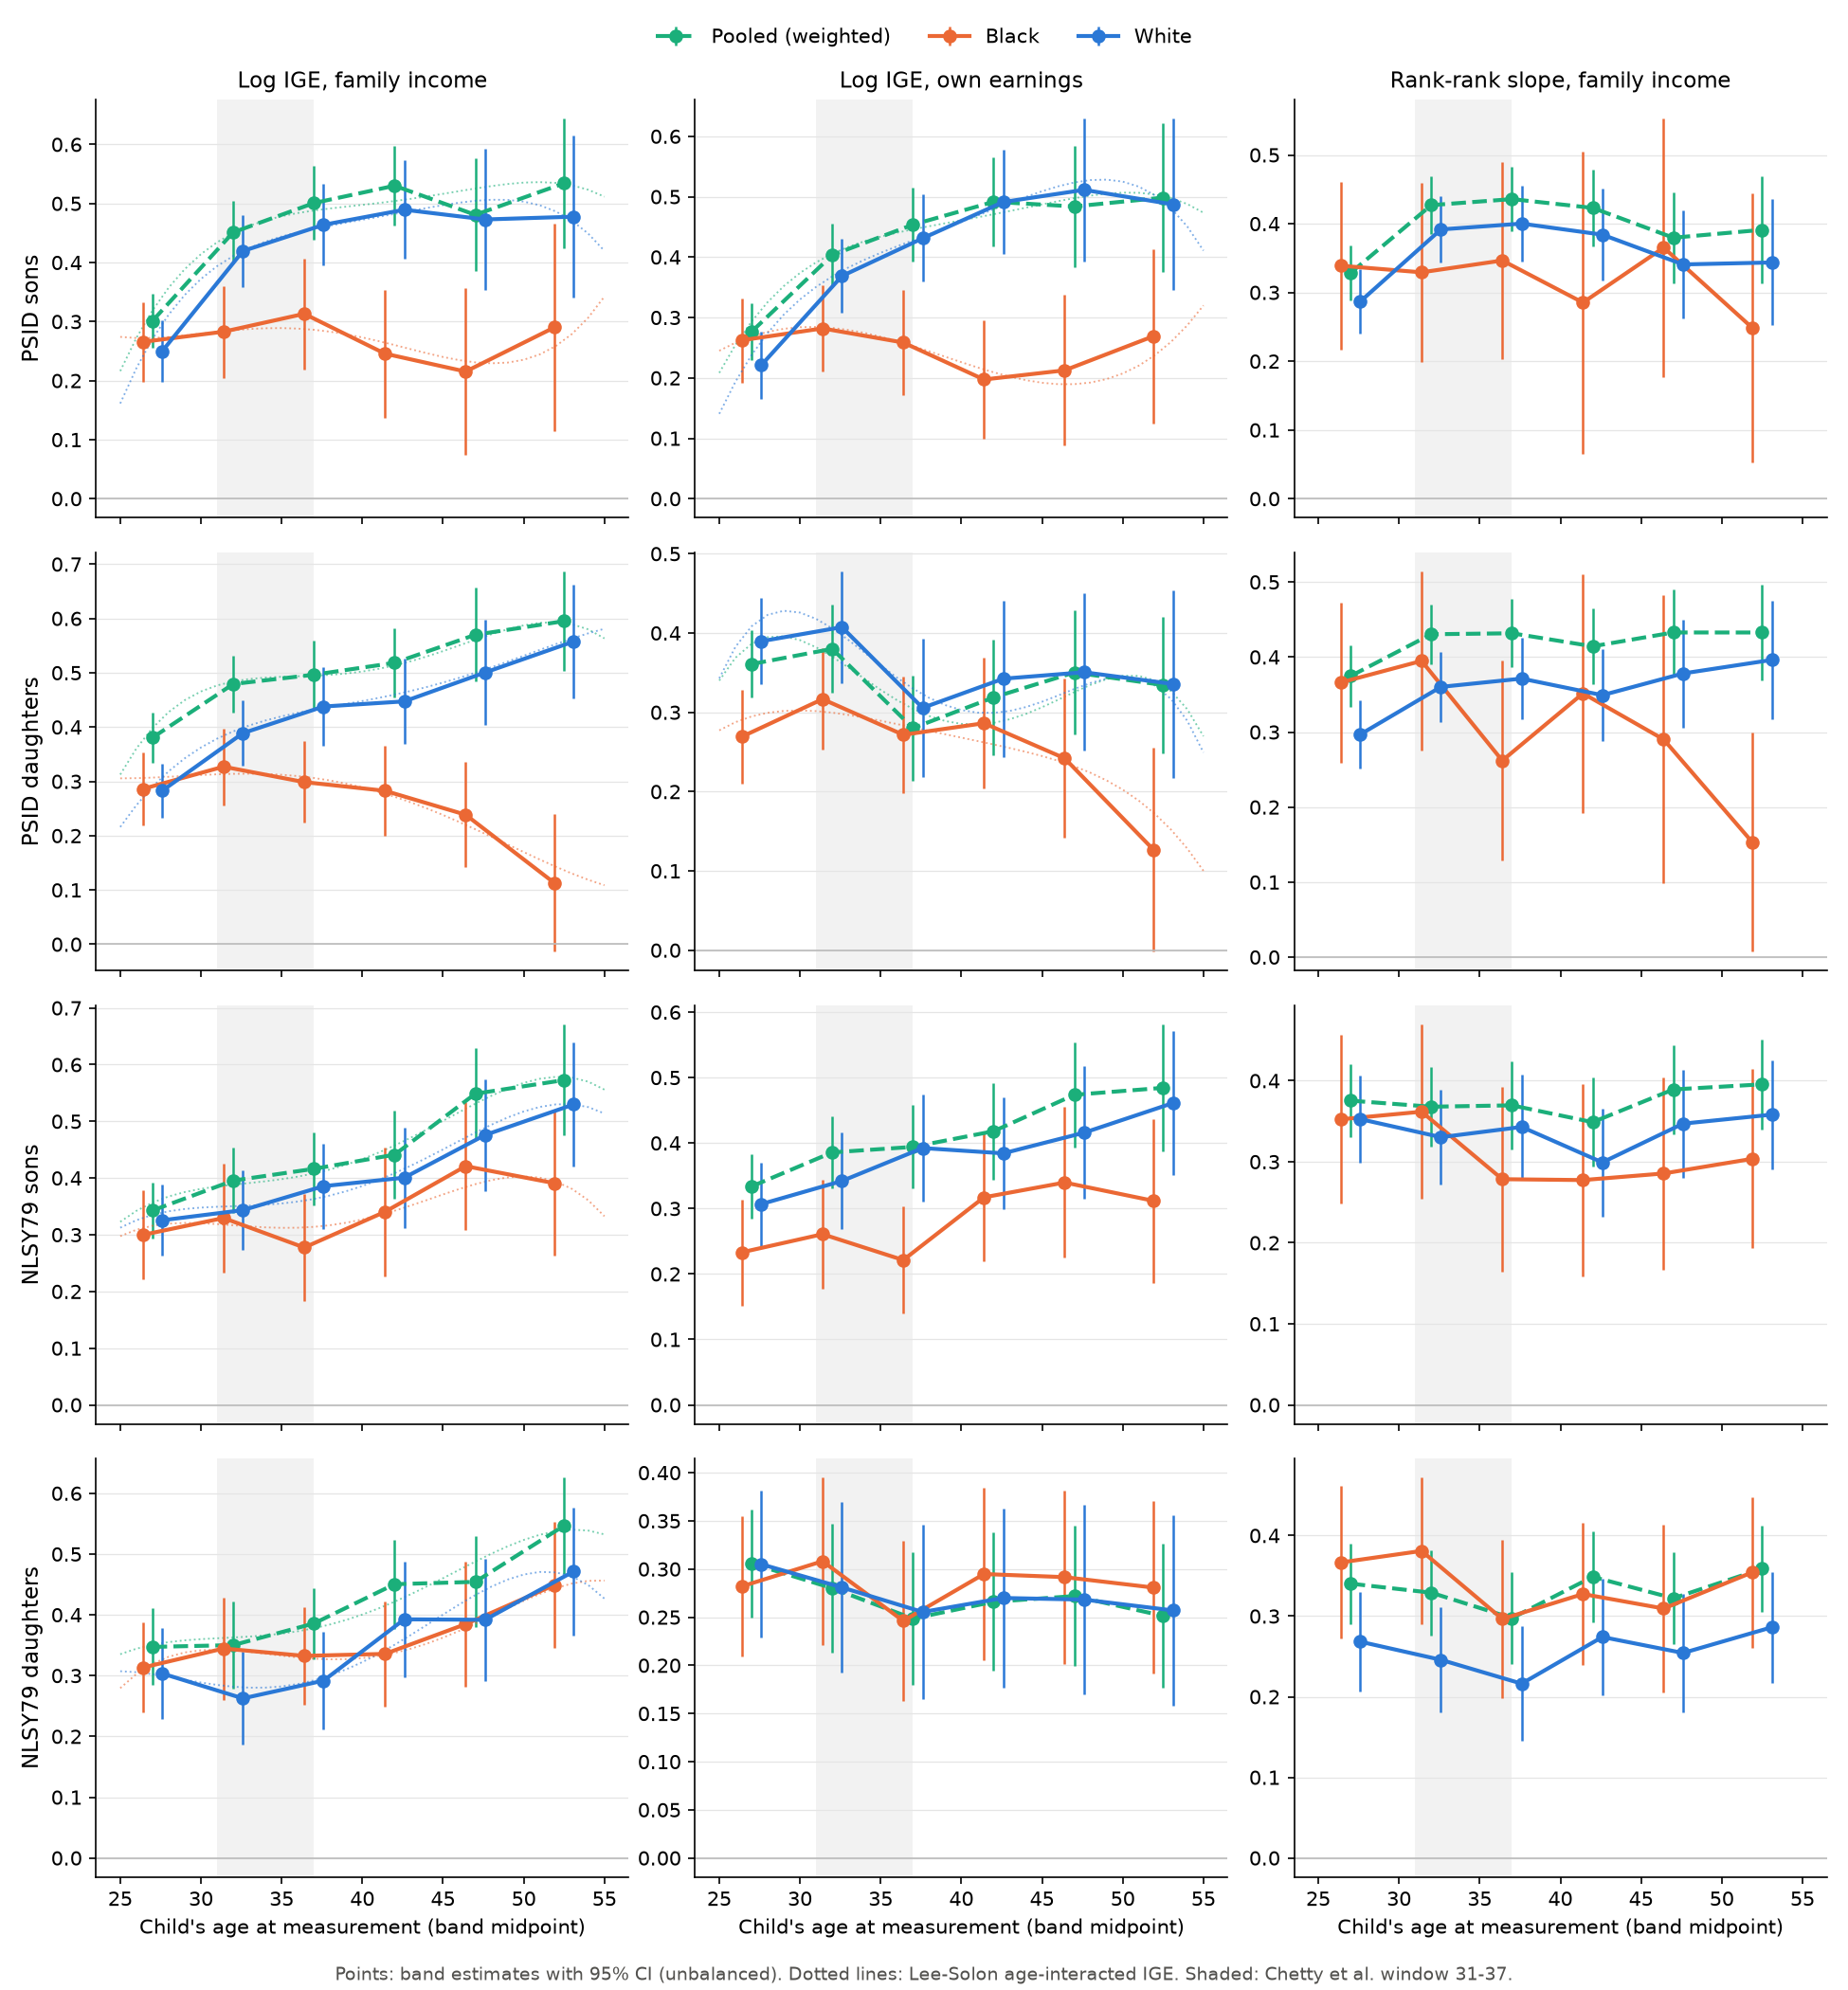
\includegraphics[width=\textwidth]{ige_by_age.png}
\caption{Intergenerational persistence by the child's age at measurement}\label{fig:ageprofile}
\begin{minipage}{\textwidth}\footnotesize \textit{Notes:} Points: band-specific estimates with 95\% confidence
intervals (unbalanced samples); dotted lines: Lee--Solon age-interacted IGE; shaded: the 31--37 window of
\citet{chetty2020race}. Columns: log IGE of family income, log IGE of own earnings, rank--rank slope of family income.
Rows: PSID sons, PSID daughters, NLSY79 sons, NLSY79 daughters. Code: \texttt{26.IGEByAge.py}.\end{minipage}
\end{figure}

\begin{table}[!htbp]
\centering
\caption{Log IGE of sons' income by age at measurement (PSID)}
\label{tab:ige_sons}
\resizebox{\ifdim\width>\textwidth\textwidth\else\width\fi}{!}{%
\resizebox*{!}{\ifdim\totalheight>0.85\textheight 0.85\textheight\else\totalheight\fi}{%
\begin{tabular}{lcc}
\toprule
Age band / group & \begin{tabular}[b]{@{}c@{}}ln own earnings\\(child-years)\end{tabular} & \begin{tabular}[b]{@{}c@{}}ln family income\\(child-years)\end{tabular} \\
 & (1) & (2) \\
\midrule
\multicolumn{3}{l}{\textit{Age 25--29}} \\
Pooled (weighted) & $0.276^{***}$ & $0.301^{***}$ \\
 & (0.024) & (0.023) \\
Black & $0.262^{***}$ & $0.266^{***}$ \\
 & (0.036) & (0.034) \\
White & $0.221^{***}$ & $0.250^{***}$ \\
 & (0.028) & (0.026) \\
White $-$ Black & $-0.041$ & $-0.016$ \\
 & (0.045) & (0.043) \\
Children (Black / White) & 1,607 / 2,474 & 1,662 / 2,506 \\
\addlinespace
\multicolumn{3}{l}{\textit{Age 30--34}} \\
Pooled (weighted) & $0.403^{***}$ & $0.451^{***}$ \\
 & (0.027) & (0.027) \\
Black & $0.282^{***}$ & $0.283^{***}$ \\
 & (0.037) & (0.040) \\
White & $0.369^{***}$ & $0.419^{***}$ \\
 & (0.031) & (0.031) \\
White $-$ Black & $0.087^{*}$ & $0.137^{***}$ \\
 & (0.048) & (0.050) \\
Children (Black / White) & 1,415 / 2,253 & 1,477 / 2,295 \\
\addlinespace
\multicolumn{3}{l}{\textit{Age 35--39}} \\
Pooled (weighted) & $0.454^{***}$ & $0.501^{***}$ \\
 & (0.031) & (0.032) \\
Black & $0.259^{***}$ & $0.313^{***}$ \\
 & (0.044) & (0.048) \\
White & $0.431^{***}$ & $0.464^{***}$ \\
 & (0.037) & (0.035) \\
White $-$ Black & $0.173^{***}$ & $0.151^{**}$ \\
 & (0.058) & (0.060) \\
Children (Black / White) & 1,068 / 1,838 & 1,125 / 1,884 \\
\addlinespace
\multicolumn{3}{l}{\textit{Age 40--44}} \\
Pooled (weighted) & $0.492^{***}$ & $0.530^{***}$ \\
 & (0.037) & (0.034) \\
Black & $0.197^{***}$ & $0.246^{***}$ \\
 & (0.050) & (0.055) \\
White & $0.491^{***}$ & $0.489^{***}$ \\
 & (0.044) & (0.043) \\
White $-$ Black & $0.294^{***}$ & $0.244^{***}$ \\
 & (0.067) & (0.070) \\
Children (Black / White) & 751 / 1,411 & 808 / 1,472 \\
\bottomrule
\end{tabular}}}
\par\smallskip
\begin{minipage}{\textwidth}\footnotesize \textit{Continued on the next table; notes below its last part.}\end{minipage}
\end{table}
\begin{table}[!htbp]
\centering
\addtocounter{table}{-1}
\caption{Log IGE of sons' income by age at measurement (PSID) (continued)}
\resizebox{\ifdim\width>\textwidth\textwidth\else\width\fi}{!}{%
\resizebox*{!}{\ifdim\totalheight>0.85\textheight 0.85\textheight\else\totalheight\fi}{%
\begin{tabular}{lcc}
\toprule
Age band / group & \begin{tabular}[b]{@{}c@{}}ln own earnings\\(child-years)\end{tabular} & \begin{tabular}[b]{@{}c@{}}ln family income\\(child-years)\end{tabular} \\
 & (1) & (2) \\
\midrule
\multicolumn{3}{l}{\textit{Age 45--49}} \\
Pooled (weighted) & $0.484^{***}$ & $0.481^{***}$ \\
 & (0.051) & (0.049) \\
Black & $0.213^{***}$ & $0.215^{***}$ \\
 & (0.064) & (0.072) \\
White & $0.511^{***}$ & $0.473^{***}$ \\
 & (0.060) & (0.061) \\
White $-$ Black & $0.299^{***}$ & $0.258^{***}$ \\
 & (0.088) & (0.095) \\
Children (Black / White) & 496 / 1,001 & 557 / 1,051 \\
\addlinespace
\multicolumn{3}{l}{\textit{Age 50--55}} \\
Pooled (weighted) & $0.498^{***}$ & $0.534^{***}$ \\
 & (0.063) & (0.056) \\
Black & $0.269^{***}$ & $0.290^{***}$ \\
 & (0.074) & (0.089) \\
White & $0.487^{***}$ & $0.478^{***}$ \\
 & (0.073) & (0.070) \\
White $-$ Black & $0.218^{**}$ & $0.187^{*}$ \\
 & (0.103) & (0.114) \\
Children (Black / White) & 351 / 726 & 420 / 780 \\
\addlinespace
\multicolumn{3}{l}{\textit{Age 31--37 (window of Chetty et al.)}} \\
Pooled (weighted) & $0.424^{***}$ & $0.475^{***}$ \\
 & (0.027) & (0.028) \\
Black & $0.292^{***}$ & $0.303^{***}$ \\
 & (0.036) & (0.041) \\
White & $0.392^{***}$ & $0.437^{***}$ \\
 & (0.032) & (0.031) \\
White $-$ Black & $0.099^{**}$ & $0.134^{***}$ \\
 & (0.048) & (0.051) \\
Children (Black / White) & 1,399 / 2,205 & 1,460 / 2,246 \\
\bottomrule
\end{tabular}}}
\par\smallskip
\begin{minipage}{\textwidth}\footnotesize \textit{Notes:} Each cell is the coefficient on log parental family income (mean over the child's ages 13--19) from a separate regression of the outcome in the column header, within the age band of the panel. Child-year columns: child-years in the band, controls for a quartic in the parent's age and single-year age dummies; band-mean columns (daughters' table; for sons in \texttt{output/ige\_by\_age.md}): one observation per child, log of the band mean ($\geq 2$ years), quartic in the parent's age and the mean age. Black and White: unweighted; Pooled: all races, weighted by the core longitudinal weight. White $-$ Black is the difference of the two race-specific regressions, estimated jointly. Standard errors clustered by 1968 family in parentheses. Race is the race of the parental household head. $^{***}$ $p<0.01$, $^{**}$ $p<0.05$, $^{*}$ $p<0.1$. Source: \texttt{26.IGEByAge.py} (\texttt{output/ige\_by\_age.csv}); table built by \texttt{28.PaperBTables.py}.\end{minipage}
\end{table}

\begin{table}[!htbp]
\centering
\caption{Who stays in the panel? Probability of being observed in a later age band (PSID)}
\label{tab:attrition}
\resizebox{\ifdim\width>\textwidth\textwidth\else\width\fi}{!}{%
\resizebox*{!}{\ifdim\totalheight>0.85\textheight 0.85\textheight\else\totalheight\fi}{%
\begin{tabular}{lcccc}
\toprule
 & \begin{tabular}[b]{@{}c@{}}30--34\end{tabular} & \begin{tabular}[b]{@{}c@{}}35--39\end{tabular} & \begin{tabular}[b]{@{}c@{}}40--44\end{tabular} & \begin{tabular}[b]{@{}c@{}}45--49\end{tabular} \\
 & (1) & (2) & (3) & (4) \\
\midrule
\multicolumn{5}{l}{\textit{Sons}} \\
Share observed, White & 0.903 & 0.799 & 0.696 & 0.584 \\
Share observed, Black & 0.809 & 0.640 & 0.521 & 0.403 \\
White: log parental income & $0.026^{**}$ & $0.068^{***}$ & $0.113^{***}$ & $0.139^{***}$ \\
 & (0.012) & (0.019) & (0.025) & (0.028) \\
Black: log parental income & $0.005$ & $-0.015$ & $-0.009$ & $0.005$ \\
 & (0.016) & (0.022) & (0.026) & (0.031) \\
White $-$ Black: log parental income & $0.021$ & $0.083^{***}$ & $0.122^{***}$ & $0.134^{***}$ \\
 & (0.020) & (0.029) & (0.036) & (0.041) \\
Children at risk & 3,767 & 3,385 & 2,912 & 2,453 \\
\addlinespace
\multicolumn{5}{l}{\textit{Daughters}} \\
Share observed, White & 0.923 & 0.835 & 0.737 & 0.612 \\
Share observed, Black & 0.886 & 0.791 & 0.703 & 0.581 \\
White: log parental income & $0.021^{**}$ & $0.031^{**}$ & $0.067^{***}$ & $0.122^{***}$ \\
 & (0.010) & (0.016) & (0.022) & (0.027) \\
Black: log parental income & $-0.009$ & $-0.016$ & $-0.031$ & $-0.012$ \\
 & (0.013) & (0.018) & (0.021) & (0.027) \\
White $-$ Black: log parental income & $0.030^{*}$ & $0.047^{**}$ & $0.098^{***}$ & $0.134^{***}$ \\
 & (0.016) & (0.024) & (0.030) & (0.038) \\
Children at risk & 4,330 & 3,851 & 3,315 & 2,764 \\
\bottomrule
\end{tabular}}}
\par\smallskip
\begin{minipage}{\textwidth}\footnotesize \textit{Notes:} Children with family income observed at 25--29 and born early enough to reach the band. Linear probability of being observed as a household head or spouse with valid family income in the band, on log parental income interacted with race, log family income at 25--29 interacted with race, a quartic in the parent's age and five-year birth-cohort dummies; standard errors clustered by 1968 family. $^{***}$ $p<0.01$, $^{**}$ $p<0.05$, $^{*}$ $p<0.1$. Source: \texttt{IGE/41.AgeProfileMeasurement.py} (\texttt{output/age\_profile\_measurement.csv}).\end{minipage}
\end{table}

\begin{table}[!htbp]
\centering
\caption{Current and lifetime income by age: Haider--Solon $\lambda$ by race (PSID, sons)}
\label{tab:lambda}
\resizebox{\ifdim\width>\textwidth\textwidth\else\width\fi}{!}{%
\resizebox*{!}{\ifdim\totalheight>0.85\textheight 0.85\textheight\else\totalheight\fi}{%
\begin{tabular}{lccccccc}
\toprule
 & \begin{tabular}[b]{@{}c@{}}25--29\end{tabular} & \begin{tabular}[b]{@{}c@{}}30--34\end{tabular} & \begin{tabular}[b]{@{}c@{}}35--39\end{tabular} & \begin{tabular}[b]{@{}c@{}}40--44\end{tabular} & \begin{tabular}[b]{@{}c@{}}45--49\end{tabular} & \begin{tabular}[b]{@{}c@{}}50--55\end{tabular} & \begin{tabular}[b]{@{}c@{}}Change, 35+\\minus below 35\end{tabular} \\
 & (1) & (2) & (3) & (4) & (5) & (6) & (7) \\
\midrule
\multicolumn{8}{l}{\textit{Own earnings}} \\
Black & $0.851^{***}$ & $0.999^{***}$ & $1.062^{***}$ & $1.123^{***}$ & $0.990^{***}$ & $1.022^{***}$ & $0.124^{*}$ \\
 & (0.076) & (0.050) & (0.060) & (0.074) & (0.055) & (0.093) & (0.072) \\
White & $0.688^{***}$ & $0.935^{***}$ & $1.051^{***}$ & $1.099^{***}$ & $1.216^{***}$ & $1.220^{***}$ & $0.335^{***}$ \\
 & (0.040) & (0.028) & (0.028) & (0.033) & (0.034) & (0.047) & (0.046) \\
White $-$ Black & $-0.163^{*}$ & $-0.064$ & $-0.011$ & $-0.024$ & $0.226^{***}$ & $0.198^{*}$ & $0.211^{**}$ \\
 & (0.086) & (0.057) & (0.066) & (0.081) & (0.065) & (0.105) & (0.086) \\
White $-$ Black, parental tercile 1 & $0.086$ & $-0.096$ & $-0.078$ & $-0.251^{**}$ & $0.361^{***}$ & $0.118$ & $0.043$ \\
 & (0.149) & (0.120) & (0.108) & (0.127) & (0.104) & (0.180) & (0.173) \\
White $-$ Black, parental tercile 2 & $-0.146$ & $-0.057$ & $-0.041$ & $0.182$ & $-0.041$ & $0.188$ & $0.173$ \\
 & (0.128) & (0.091) & (0.146) & (0.117) & (0.113) & (0.137) & (0.134) \\
White $-$ Black, parental tercile 3 & $-0.286^{**}$ & $0.124$ & $0.098$ & $0.289^{**}$ & $-0.174$ & $0.072$ & $0.153$ \\
 & (0.136) & (0.137) & (0.129) & (0.136) & (0.109) & (0.162) & (0.144) \\
Sons (Black / White) & 267 / 676 &  &  &  &  &  &  \\
\addlinespace
\multicolumn{8}{l}{\textit{Family income}} \\
Black & $0.817^{***}$ & $0.970^{***}$ & $1.052^{***}$ & $1.134^{***}$ & $1.096^{***}$ & $1.025^{***}$ & $0.183^{***}$ \\
 & (0.044) & (0.038) & (0.043) & (0.040) & (0.048) & (0.058) & (0.044) \\
White & $0.698^{***}$ & $0.894^{***}$ & $1.049^{***}$ & $1.067^{***}$ & $1.238^{***}$ & $1.280^{***}$ & $0.363^{***}$ \\
 & (0.030) & (0.027) & (0.027) & (0.026) & (0.033) & (0.040) & (0.037) \\
White $-$ Black & $-0.118^{**}$ & $-0.077$ & $-0.003$ & $-0.067$ & $0.142^{**}$ & $0.255^{***}$ & $0.179^{***}$ \\
 & (0.054) & (0.047) & (0.051) & (0.048) & (0.058) & (0.070) & (0.057) \\
White $-$ Black, parental tercile 1 & $0.105$ & $-0.135$ & $-0.102$ & $-0.185^{*}$ & $0.158$ & $0.264^{**}$ & $0.049$ \\
 & (0.104) & (0.129) & (0.090) & (0.095) & (0.108) & (0.107) & (0.133) \\
White $-$ Black, parental tercile 2 & $-0.106$ & $-0.088$ & $-0.006$ & $0.005$ & $0.013$ & $0.210^{*}$ & $0.153$ \\
 & (0.080) & (0.087) & (0.109) & (0.094) & (0.096) & (0.115) & (0.100) \\
White $-$ Black, parental tercile 3 & $-0.227^{**}$ & $0.009$ & $0.037$ & $0.195^{*}$ & $-0.050$ & $0.178$ & $0.199$ \\
 & (0.110) & (0.095) & (0.098) & (0.118) & (0.119) & (0.122) & (0.145) \\
Sons (Black / White) & 326 / 734 &  &  &  &  &  &  \\
\bottomrule
\end{tabular}}}
\par\smallskip
\begin{minipage}{\textwidth}\footnotesize \textit{Notes:} Sons with at least three valid years in each of 25--34, 35--44 and 45--55. $\lambda$: slope of the log outcome in the band (net of race-specific single-age means) on the son's mean of the same net log outcome over 25--55, by race, with single-age dummies; standard errors clustered by 1968 family. Adding log parental income to these regressions leaves $\lambda$ unchanged and its coefficient is not different from zero in any band (\texttt{output/age\_profile\_measurement.md}, Section C). $^{***}$ $p<0.01$, $^{**}$ $p<0.05$, $^{*}$ $p<0.1$. Source: \texttt{41.AgeProfileMeasurement.py} (\texttt{output/age\_profile\_measurement.csv}).\end{minipage}
\end{table}

\begin{table}[!htbp]
\centering
\caption{The racial gap in the log IGE by potential experience (PSID, sons)}
\label{tab:experience}
\resizebox{\ifdim\width>\textwidth\textwidth\else\width\fi}{!}{%
\resizebox*{!}{\ifdim\totalheight>0.85\textheight 0.85\textheight\else\totalheight\fi}{%
\begin{tabular}{lcccccc}
\toprule
 & \begin{tabular}[b]{@{}c@{}}0--4\end{tabular} & \begin{tabular}[b]{@{}c@{}}5--9\end{tabular} & \begin{tabular}[b]{@{}c@{}}10--14\end{tabular} & \begin{tabular}[b]{@{}c@{}}15--19\end{tabular} & \begin{tabular}[b]{@{}c@{}}20--24\end{tabular} & \begin{tabular}[b]{@{}c@{}}Opening\\($\geq$10 minus $<$10)\end{tabular} \\
 & (1) & (2) & (3) & (4) & (5) & (6) \\
\midrule
\multicolumn{7}{l}{\textit{Controls: single-year experience dummies}} \\
White $-$ Black gap, own earnings & $-0.121$ & $0.043$ & $0.118^{**}$ & $0.220^{***}$ & $0.272^{***}$ & $0.243^{***}$ \\
 & (0.101) & (0.044) & (0.051) & (0.059) & (0.066) & (0.067) \\
White $-$ Black gap, family income & $-0.100$ & $0.065$ & $0.168^{***}$ & $0.246^{***}$ & $0.216^{***}$ & $0.227^{***}$ \\
 & (0.093) & (0.044) & (0.052) & (0.060) & (0.071) & (0.065) \\
\addlinespace
\multicolumn{7}{l}{\textit{Controls: single-year age dummies}} \\
White $-$ Black gap, own earnings & $-0.123$ & $0.003$ & $0.059$ & $0.154^{***}$ & $0.196^{***}$ & $0.197^{***}$ \\
 & (0.099) & (0.043) & (0.046) & (0.055) & (0.063) & (0.064) \\
White $-$ Black gap, family income & $-0.099$ & $0.009$ & $0.094^{**}$ & $0.178^{***}$ & $0.143^{**}$ & $0.183^{***}$ \\
 & (0.092) & (0.043) & (0.047) & (0.056) & (0.067) & (0.062) \\
\bottomrule
\end{tabular}}}
\par\smallskip
\begin{minipage}{\textwidth}\footnotesize \textit{Notes:} Child-years at ages 20--55 as head or spouse, bands of potential experience (age $-$ completed years of schooling $-$ 6). Each cell: White $-$ Black difference of the band-specific log IGEs (stacked, clustered by 1968 family); controls: quartic in the parent's age and single-year age or experience dummies. At 25--29, sons of top-tercile White parents have 4.8 years of potential experience, other sons 6.0--7.0. $^{***}$ $p<0.01$, $^{**}$ $p<0.05$, $^{*}$ $p<0.1$. Source: \texttt{46.AgeProfileRound2.py} (\texttt{output/age\_profile\_round2.md}).\end{minipage}
\end{table}

\begin{table}[!htbp]
\centering
\caption{Schooling and ability: growth within cells and returns by age}
\label{tab:afqtgrowth}
\resizebox{\ifdim\width>\textwidth\textwidth\else\width\fi}{!}{%
\resizebox*{!}{\ifdim\totalheight>0.85\textheight 0.85\textheight\else\totalheight\fi}{%
\begin{tabular}{lccc}
\toprule
 & \begin{tabular}[b]{@{}c@{}}(1)\end{tabular} & \begin{tabular}[b]{@{}c@{}}(2)\end{tabular} & \begin{tabular}[b]{@{}c@{}}(3)\end{tabular} \\
 & (1) & (2) & (3) \\
\midrule
\multicolumn{4}{l}{\textit{PSID: same-employer wage growth at 25--34 on years of schooling}} \\
White & $0.010^{***}$ & $0.007^{***}$ & $0.009^{***}$ \\
 & (0.002) & (0.002) & (0.002) \\
Black & $0.003$ & $0.003$ & $0.001$ \\
 & (0.003) & (0.004) & (0.004) \\
White $-$ Black & $0.007^{**}$ & $0.004$ & $0.008$ \\
 & (0.003) & (0.005) & (0.005) \\
\addlinespace
\multicolumn{4}{l}{\textit{NLSY79: same-employer wage growth at 25--34 on years of schooling}} \\
White & $0.004^{***}$ & $0.004^{**}$ & $0.002$ \\
 & (0.001) & (0.001) & (0.001) \\
Black & $0.003$ & $-0.001$ & $-0.002$ \\
 & (0.002) & (0.002) & (0.003) \\
White $-$ Black & $0.002$ & $0.005^{*}$ & $0.004$ \\
 & (0.002) & (0.003) & (0.003) \\
\addlinespace
\multicolumn{4}{l}{\textit{NLSY79: log hourly rate of pay on AFQT (1 s.d.), by age}} \\
White: return to AFQT (1 s.d.) at 25--29 & $0.140^{***}$ &  & $0.103^{***}$ \\
 & (0.010) &  & (0.014) \\
White: rise of the return to AFQT (1 s.d.) & $0.110^{***}$ &  & $0.021^{*}$ \\
 & (0.010) &  & (0.013) \\
Black: return to AFQT (1 s.d.) at 25--29 & $0.188^{***}$ &  & $0.121^{***}$ \\
 & (0.017) &  & (0.020) \\
Black: rise of the return to AFQT (1 s.d.) & $0.098^{***}$ &  & $0.053^{**}$ \\
 & (0.019) &  & (0.022) \\
White $-$ Black: return to AFQT (1 s.d.) at 25--29 & $-0.048^{**}$ &  & $-0.018$ \\
 & (0.020) &  & (0.024) \\
White $-$ Black: rise of the return to AFQT (1 s.d.) & $0.012$ &  & $-0.031$ \\
 & (0.022) &  & (0.025) \\
\addlinespace
\multicolumn{4}{l}{\textit{NLSY79: log hourly rate of pay on years of schooling, by age}} \\
White: return to years of schooling at 25--29 &  & $0.048^{***}$ & $0.022^{***}$ \\
 &  & (0.004) & (0.005) \\
White: rise of the return to years of schooling &  & $0.057^{***}$ & $0.052^{***}$ \\
 &  & (0.004) & (0.005) \\
Black: return to years of schooling at 25--29 &  & $0.069^{***}$ & $0.043^{***}$ \\
 &  & (0.006) & (0.007) \\
Black: rise of the return to years of schooling &  & $0.042^{***}$ & $0.030^{***}$ \\
 &  & (0.006) & (0.007) \\
White $-$ Black: return to years of schooling at 25--29 &  & $-0.022^{***}$ & $-0.022^{**}$ \\
 &  & (0.007) & (0.008) \\
White $-$ Black: rise of the return to years of schooling &  & $0.015^{*}$ & $0.021^{**}$ \\
 &  & (0.008) & (0.009) \\
\bottomrule
\end{tabular}}}
\par\smallskip
\begin{minipage}{\textwidth}\footnotesize \textit{Notes:} Top panels: same-employer pairs at 25--34 (Table~\ref{tab:growthladder}); columns: (1) no cell controls, (2) fixed effects for the occupation group $\times$ industry group at the first interview of the pair, (3) for the early cell. Bottom panels: NLSY79 men 25--55, log hourly rate of pay on the AFQT (standardised within birth year) alone (1), schooling alone (2) or both (3), by age band; rise = mean over bands from 35 minus mean below 35. Employer learning predicts that with both included the schooling coefficient falls and the AFQT coefficient rises with experience. Controls: quartic in age, year (round) fixed effects. $^{***}$ $p<0.01$, $^{**}$ $p<0.05$, $^{*}$ $p<0.1$. Source: \texttt{45.WithinCellIdentification.py}.\end{minipage}
\end{table}

\begin{table}[!htbp]
\centering
\caption{Rank mobility of sons by age at measurement (PSID)}
\label{tab:rankage}
\resizebox{\ifdim\width>\textwidth\textwidth\else\width\fi}{!}{%
\resizebox*{!}{\ifdim\totalheight>0.85\textheight 0.85\textheight\else\totalheight\fi}{%
\begin{tabular}{lcccc}
\toprule
Age band / group & \begin{tabular}[b]{@{}c@{}}Rank--rank slope\\family income\end{tabular} & \begin{tabular}[b]{@{}c@{}}Expected rank\\at parental p25\end{tabular} & \begin{tabular}[b]{@{}c@{}}Expected rank\\at parental p75\end{tabular} & \begin{tabular}[b]{@{}c@{}}Rank--rank slope\\own earnings\end{tabular} \\
 & (1) & (2) & (3) & (4) \\
\midrule
\multicolumn{5}{l}{\textit{Age 25--29}} \\
Pooled (weighted) & $0.328^{***}$ & $40.7^{***}$ & $57.1^{***}$ & $0.300^{***}$ \\
 & (0.020) & (0.8) & (0.8) & (0.021) \\
Black & $0.339^{***}$ & $32.3^{***}$ & $49.2$ & $0.261^{***}$ \\
 & (0.062) & (1.3) & (3.5) & (0.067) \\
White & $0.287^{***}$ & $43.3^{***}$ & $57.6^{***}$ & $0.253^{***}$ \\
 & (0.024) & (1.0) & (0.8) & (0.023) \\
White $-$ Black & $-0.052$ & $11.0^{***}$ & $8.4^{**}$ & $-0.008$ \\
 & (0.067) & (1.6) & (3.6) & (0.071) \\
Children (Black / White) & 1,242 / 2,098 & 1,242 / 2,098 & 1,242 / 2,098 & 1,242 / 2,098 \\
\addlinespace
\multicolumn{5}{l}{\textit{Age 30--34}} \\
Pooled (weighted) & $0.427^{***}$ & $38.7^{***}$ & $60.1^{***}$ & $0.366^{***}$ \\
 & (0.022) & (0.9) & (0.8) & (0.020) \\
Black & $0.329^{***}$ & $31.3^{***}$ & $47.8$ & $0.299^{***}$ \\
 & (0.067) & (1.6) & (3.3) & (0.057) \\
White & $0.392^{***}$ & $41.1^{***}$ & $60.7^{***}$ & $0.322^{***}$ \\
 & (0.025) & (1.0) & (0.8) & (0.023) \\
White $-$ Black & $0.062$ & $9.8^{***}$ & $12.9^{***}$ & $0.024$ \\
 & (0.071) & (1.9) & (3.4) & (0.061) \\
Children (Black / White) & 1,141 / 1,932 & 1,141 / 1,932 & 1,141 / 1,932 & 1,141 / 1,932 \\
\addlinespace
\multicolumn{5}{l}{\textit{Age 35--39}} \\
Pooled (weighted) & $0.436^{***}$ & $38.9^{***}$ & $60.7^{***}$ & $0.356^{***}$ \\
 & (0.024) & (0.9) & (0.8) & (0.021) \\
Black & $0.346^{***}$ & $32.3^{***}$ & $49.6$ & $0.279^{***}$ \\
 & (0.073) & (1.5) & (3.9) & (0.065) \\
White & $0.400^{***}$ & $41.0^{***}$ & $61.0^{***}$ & $0.325^{***}$ \\
 & (0.028) & (1.2) & (0.9) & (0.025) \\
White $-$ Black & $0.054$ & $8.7^{***}$ & $11.4^{***}$ & $0.046$ \\
 & (0.079) & (1.9) & (4.0) & (0.069) \\
Children (Black / White) & 875 / 1,569 & 875 / 1,569 & 875 / 1,569 & 875 / 1,569 \\
\addlinespace
\multicolumn{5}{l}{\textit{Age 40--44}} \\
Pooled (weighted) & $0.423^{***}$ & $38.7^{***}$ & $59.8^{***}$ & $0.368^{***}$ \\
 & (0.028) & (1.2) & (1.0) & (0.027) \\
Black & $0.285^{**}$ & $32.7^{***}$ & $47.0$ & $0.202^{***}$ \\
 & (0.112) & (1.9) & (6.6) & (0.077) \\
White & $0.384^{***}$ & $40.7^{***}$ & $59.9^{***}$ & $0.352^{***}$ \\
 & (0.034) & (1.5) & (1.0) & (0.032) \\
White $-$ Black & $0.099$ & $8.0^{***}$ & $12.9^{*}$ & $0.150^{*}$ \\
 & (0.117) & (2.4) & (6.7) & (0.083) \\
Children (Black / White) & 572 / 1,175 & 572 / 1,175 & 572 / 1,175 & 572 / 1,175 \\
\bottomrule
\end{tabular}}}
\par\smallskip
\begin{minipage}{\textwidth}\footnotesize \textit{Continued on the next table; notes below its last part.}\end{minipage}
\end{table}
\begin{table}[!htbp]
\centering
\addtocounter{table}{-1}
\caption{Rank mobility of sons by age at measurement (PSID) (continued)}
\resizebox{\ifdim\width>\textwidth\textwidth\else\width\fi}{!}{%
\resizebox*{!}{\ifdim\totalheight>0.85\textheight 0.85\textheight\else\totalheight\fi}{%
\begin{tabular}{lcccc}
\toprule
Age band / group & \begin{tabular}[b]{@{}c@{}}Rank--rank slope\\family income\end{tabular} & \begin{tabular}[b]{@{}c@{}}Expected rank\\at parental p25\end{tabular} & \begin{tabular}[b]{@{}c@{}}Expected rank\\at parental p75\end{tabular} & \begin{tabular}[b]{@{}c@{}}Rank--rank slope\\own earnings\end{tabular} \\
 & (1) & (2) & (3) & (4) \\
\midrule
\multicolumn{5}{l}{\textit{Age 45--49}} \\
Pooled (weighted) & $0.380^{***}$ & $40.4^{***}$ & $59.3^{***}$ & $0.336^{***}$ \\
 & (0.034) & (1.4) & (1.2) & (0.034) \\
Black & $0.365^{***}$ & $34.4^{***}$ & $52.7$ & $0.258^{***}$ \\
 & (0.096) & (2.6) & (5.5) & (0.098) \\
White & $0.341^{***}$ & $42.4^{***}$ & $59.4^{***}$ & $0.314^{***}$ \\
 & (0.040) & (1.7) & (1.2) & (0.039) \\
White $-$ Black & $-0.024$ & $8.0^{**}$ & $6.7$ & $0.056$ \\
 & (0.104) & (3.1) & (5.7) & (0.106) \\
Children (Black / White) & 405 / 821 & 405 / 821 & 405 / 821 & 405 / 821 \\
\addlinespace
\multicolumn{5}{l}{\textit{Age 50--55}} \\
Pooled (weighted) & $0.391^{***}$ & $40.5^{***}$ & $60.0^{***}$ & $0.350^{***}$ \\
 & (0.040) & (1.6) & (1.4) & (0.041) \\
Black & $0.248^{**}$ & $32.0^{***}$ & $44.4$ & $0.213^{*}$ \\
 & (0.100) & (2.0) & (5.4) & (0.113) \\
White & $0.344^{***}$ & $42.8^{***}$ & $60.0^{***}$ & $0.317^{***}$ \\
 & (0.047) & (1.9) & (1.5) & (0.048) \\
White $-$ Black & $0.095$ & $10.8^{***}$ & $15.6^{***}$ & $0.104$ \\
 & (0.110) & (2.8) & (5.6) & (0.123) \\
Children (Black / White) & 339 / 613 & 339 / 613 & 339 / 613 & 339 / 613 \\
\addlinespace
\multicolumn{5}{l}{\textit{Age 31--37 (window of Chetty et al.)}} \\
Pooled (weighted) & $0.442^{***}$ & $38.7^{***}$ & $60.8^{***}$ & $0.372^{***}$ \\
 & (0.022) & (0.9) & (0.8) & (0.020) \\
Black & $0.348^{***}$ & $30.3^{***}$ & $47.7$ & $0.308^{***}$ \\
 & (0.064) & (1.5) & (3.2) & (0.061) \\
White & $0.397^{***}$ & $41.5^{***}$ & $61.3^{***}$ & $0.324^{***}$ \\
 & (0.025) & (1.0) & (0.8) & (0.022) \\
White $-$ Black & $0.048$ & $11.2^{***}$ & $13.6^{***}$ & $0.017$ \\
 & (0.069) & (1.8) & (3.3) & (0.065) \\
Children (Black / White) & 1,179 / 1,924 & 1,179 / 1,924 & 1,179 / 1,924 & 1,179 / 1,924 \\
\addlinespace
\multicolumn{5}{l}{\textit{Tests on the White $-$ Black slope gap across bands 25--29 to 50--55}} \\
Equal in all bands: Wald $\chi^2$ [p-value] & $\chi^2(5)=5.17$ &  &  & $\chi^2(5)=4.13$ \\
 & [0.396] &  &  & [0.530] \\
Linear trend per 10 years of age & $0.030$ &  &  & $0.043$ \\
 & (0.044) &  &  & (0.047) \\
\bottomrule
\end{tabular}}}
\par\smallskip
\begin{minipage}{\textwidth}\footnotesize \textit{Notes:} Child's band-mean family income (columns 1--3) or own earnings (column 4, zeros kept) ranked within birth year and band; parents' family income (mean at the child's ages 12--17) ranked within the child's birth year. Columns (2) and (3) evaluate the rank--rank line of column (1) at the 25th and 75th parental percentiles. All rank statistics weighted (core longitudinal weight at 16). Standard errors clustered by 1968 family in parentheses. $^{***}$ $p<0.01$, $^{**}$ $p<0.05$, $^{*}$ $p<0.1$. Source: \texttt{26.IGEByAge.py} (\texttt{output/ige\_by\_age.csv}); table built by \texttt{28.PaperBTables.py}.\end{minipage}
\end{table}

\begin{table}[!htbp]
\centering
\caption{Income growth by parental income: the same sons observed early and late (PSID)}
\label{tab:growth}
\resizebox{\ifdim\width>\textwidth\textwidth\else\width\fi}{!}{%
\resizebox*{!}{\ifdim\totalheight>0.85\textheight 0.85\textheight\else\totalheight\fi}{%
\begin{tabular}{lcccccc}
\toprule
Panel / group & \begin{tabular}[b]{@{}c@{}}ln family income\\early band\end{tabular} & \begin{tabular}[b]{@{}c@{}}ln family income\\late band\end{tabular} & \begin{tabular}[b]{@{}c@{}}Growth\\(late $-$ early)\end{tabular} & \begin{tabular}[b]{@{}c@{}}ln own earnings\\early band\end{tabular} & \begin{tabular}[b]{@{}c@{}}ln own earnings\\late band\end{tabular} & \begin{tabular}[b]{@{}c@{}}Growth\\(late $-$ early)\end{tabular} \\
 & (1) & (2) & (3) & (4) & (5) & (6) \\
\midrule
\multicolumn{7}{l}{\textit{Early band 25--29, late band 35--39}} \\
Pooled (weighted) & $0.310^{***}$ & $0.519^{***}$ & $0.210^{***}$ & $0.265^{***}$ & $0.465^{***}$ & $0.200^{***}$ \\
 & (0.028) & (0.034) & (0.031) & (0.029) & (0.035) & (0.035) \\
Black & $0.250^{***}$ & $0.376^{***}$ & $0.121^{***}$ & $0.262^{***}$ & $0.348^{***}$ & $0.085^{*}$ \\
 & (0.045) & (0.052) & (0.045) & (0.047) & (0.052) & (0.044) \\
White & $0.258^{***}$ & $0.473^{***}$ & $0.216^{***}$ & $0.211^{***}$ & $0.430^{***}$ & $0.219^{***}$ \\
 & (0.031) & (0.035) & (0.031) & (0.034) & (0.037) & (0.038) \\
White $-$ Black & $0.008$ & $0.097$ & $0.096^{*}$ & $-0.051$ & $0.081$ & $0.134^{**}$ \\
 & (0.055) & (0.063) & (0.055) & (0.058) & (0.064) & (0.058) \\
Children (Black / White) & 893 / 1,713 & 893 / 1,713 & 893 / 1,713 & 840 / 1,666 & 840 / 1,666 & 840 / 1,666 \\
\addlinespace
\multicolumn{7}{l}{\textit{Early band 25--29, late band 45--49}} \\
Pooled (weighted) & $0.337^{***}$ & $0.475^{***}$ & $0.146^{***}$ & $0.266^{***}$ & $0.477^{***}$ & $0.213^{***}$ \\
 & (0.038) & (0.052) & (0.047) & (0.040) & (0.064) & (0.055) \\
Black & $0.219^{***}$ & $0.189^{**}$ & $-0.030$ & $0.178^{***}$ & $0.166^{*}$ & $-0.011$ \\
 & (0.061) & (0.091) & (0.073) & (0.061) & (0.088) & (0.061) \\
White & $0.294^{***}$ & $0.464^{***}$ & $0.182^{***}$ & $0.245^{***}$ & $0.515^{***}$ & $0.273^{***}$ \\
 & (0.043) & (0.064) & (0.053) & (0.046) & (0.073) & (0.060) \\
White $-$ Black & $0.075$ & $0.275^{**}$ & $0.212^{**}$ & $0.067$ & $0.349^{***}$ & $0.284^{***}$ \\
 & (0.075) & (0.111) & (0.090) & (0.076) & (0.114) & (0.086) \\
Children (Black / White) & 423 / 938 & 423 / 938 & 423 / 938 & 371 / 896 & 371 / 896 & 371 / 896 \\
\addlinespace
\multicolumn{7}{l}{\textit{Early band 30--34, late band 40--44}} \\
Pooled (weighted) & $0.471^{***}$ & $0.491^{***}$ & $0.021$ & $0.431^{***}$ & $0.480^{***}$ & $0.050$ \\
 & (0.041) & (0.039) & (0.036) & (0.041) & (0.044) & (0.039) \\
Black & $0.271^{***}$ & $0.273^{***}$ & $0.003$ & $0.238^{***}$ & $0.253^{***}$ & $0.020$ \\
 & (0.061) & (0.059) & (0.064) & (0.055) & (0.058) & (0.049) \\
White & $0.445^{***}$ & $0.473^{***}$ & $0.027$ & $0.399^{***}$ & $0.465^{***}$ & $0.066^{*}$ \\
 & (0.040) & (0.045) & (0.036) & (0.041) & (0.045) & (0.036) \\
White $-$ Black & $0.174^{**}$ & $0.200^{***}$ & $0.025$ & $0.161^{**}$ & $0.212^{***}$ & $0.045$ \\
 & (0.073) & (0.074) & (0.073) & (0.069) & (0.073) & (0.060) \\
Children (Black / White) & 703 / 1,398 & 703 / 1,398 & 703 / 1,398 & 644 / 1,335 & 644 / 1,335 & 644 / 1,335 \\
\bottomrule
\end{tabular}}}
\par\smallskip
\begin{minipage}{\textwidth}\footnotesize \textit{Notes:} One observation per son observed in both bands of the panel. Columns (1), (2), (4), (5): the band-mean outcome on log parental income; columns (3) and (6): the change in the band-mean outcome on log parental income (controls: quartic in the parent's age and the change in mean age). A positive growth coefficient means that sons of richer parents have steeper income growth between the two bands, which raises the IGE measured later in life \citep{haider2006life}. Standard errors clustered by 1968 family. $^{***}$ $p<0.01$, $^{**}$ $p<0.05$, $^{*}$ $p<0.1$. Source: \texttt{IGE/26.IGEByAge.py} (\texttt{output/ige\_by\_age.csv}); table built by \texttt{IGE/28.PaperBTables.py}.\end{minipage}
\end{table}

\begin{table}[!htbp]
\centering
\caption{Log IGE of daughters' income by age at measurement (PSID)}
\label{tab:ige_daughters}
\resizebox{\ifdim\width>\textwidth\textwidth\else\width\fi}{!}{%
\resizebox*{!}{\ifdim\totalheight>0.85\textheight 0.85\textheight\else\totalheight\fi}{%
\begin{tabular}{lcccc}
\toprule
Age band / group & \begin{tabular}[b]{@{}c@{}}ln own earnings\\(child-years)\end{tabular} & \begin{tabular}[b]{@{}c@{}}ln family income\\(child-years)\end{tabular} & \begin{tabular}[b]{@{}c@{}}ln own earnings\\(band mean)\end{tabular} & \begin{tabular}[b]{@{}c@{}}ln family income\\(band mean)\end{tabular} \\
 & (1) & (2) & (3) & (4) \\
\midrule
\multicolumn{5}{l}{\textit{Age 25--29}} \\
Pooled (weighted) & $0.361^{***}$ & $0.381^{***}$ & $0.346^{***}$ & $0.359^{***}$ \\
 & (0.022) & (0.023) & (0.022) & (0.022) \\
Black & $0.269^{***}$ & $0.286^{***}$ & $0.263^{***}$ & $0.291^{***}$ \\
 & (0.030) & (0.034) & (0.031) & (0.031) \\
White & $0.390^{***}$ & $0.283^{***}$ & $0.375^{***}$ & $0.274^{***}$ \\
 & (0.028) & (0.025) & (0.026) & (0.025) \\
White $-$ Black & $0.120^{***}$ & $-0.003$ & $0.112^{***}$ & $-0.017$ \\
 & (0.041) & (0.042) & (0.040) & (0.039) \\
Children (Black / White) & 1,888 / 2,540 & 2,085 / 2,702 & 1,502 / 2,176 & 1,812 / 2,474 \\
\addlinespace
\multicolumn{5}{l}{\textit{Age 30--34}} \\
Pooled (weighted) & $0.380^{***}$ & $0.479^{***}$ & $0.376^{***}$ & $0.464^{***}$ \\
 & (0.028) & (0.027) & (0.027) & (0.024) \\
Black & $0.317^{***}$ & $0.327^{***}$ & $0.294^{***}$ & $0.321^{***}$ \\
 & (0.033) & (0.036) & (0.030) & (0.033) \\
White & $0.407^{***}$ & $0.389^{***}$ & $0.425^{***}$ & $0.387^{***}$ \\
 & (0.036) & (0.030) & (0.033) & (0.028) \\
White $-$ Black & $0.091^{*}$ & $0.062$ & $0.131^{***}$ & $0.065$ \\
 & (0.048) & (0.047) & (0.045) & (0.043) \\
Children (Black / White) & 1,715 / 2,222 & 1,882 / 2,428 & 1,393 / 1,884 & 1,670 / 2,227 \\
\addlinespace
\multicolumn{5}{l}{\textit{Age 35--39}} \\
Pooled (weighted) & $0.280^{***}$ & $0.496^{***}$ & $0.302^{***}$ & $0.473^{***}$ \\
 & (0.034) & (0.032) & (0.034) & (0.029) \\
Black & $0.272^{***}$ & $0.299^{***}$ & $0.261^{***}$ & $0.271^{***}$ \\
 & (0.038) & (0.038) & (0.036) & (0.035) \\
White & $0.306^{***}$ & $0.438^{***}$ & $0.349^{***}$ & $0.434^{***}$ \\
 & (0.044) & (0.037) & (0.043) & (0.034) \\
White $-$ Black & $0.034$ & $0.139^{***}$ & $0.088$ & $0.163^{***}$ \\
 & (0.058) & (0.053) & (0.057) & (0.049) \\
Children (Black / White) & 1,431 / 1,836 & 1,580 / 2,040 & 1,152 / 1,509 & 1,379 / 1,812 \\
\addlinespace
\multicolumn{5}{l}{\textit{Age 40--44}} \\
Pooled (weighted) & $0.319^{***}$ & $0.518^{***}$ & $0.312^{***}$ & $0.502^{***}$ \\
 & (0.037) & (0.032) & (0.036) & (0.032) \\
Black & $0.286^{***}$ & $0.283^{***}$ & $0.258^{***}$ & $0.291^{***}$ \\
 & (0.042) & (0.042) & (0.040) & (0.041) \\
White & $0.342^{***}$ & $0.447^{***}$ & $0.358^{***}$ & $0.434^{***}$ \\
 & (0.050) & (0.040) & (0.048) & (0.039) \\
White $-$ Black & $0.056$ & $0.165^{***}$ & $0.100$ & $0.143^{**}$ \\
 & (0.066) & (0.058) & (0.063) & (0.056) \\
Children (Black / White) & 1,107 / 1,403 & 1,260 / 1,587 & 856 / 1,144 & 1,066 / 1,373 \\
\bottomrule
\end{tabular}}}
\par\smallskip
\begin{minipage}{\textwidth}\footnotesize \textit{Continued on the next table; notes below its last part.}\end{minipage}
\end{table}
\begin{table}[!htbp]
\centering
\addtocounter{table}{-1}
\caption{Log IGE of daughters' income by age at measurement (PSID) (continued)}
\resizebox{\ifdim\width>\textwidth\textwidth\else\width\fi}{!}{%
\resizebox*{!}{\ifdim\totalheight>0.85\textheight 0.85\textheight\else\totalheight\fi}{%
\begin{tabular}{lcccc}
\toprule
Age band / group & \begin{tabular}[b]{@{}c@{}}ln own earnings\\(child-years)\end{tabular} & \begin{tabular}[b]{@{}c@{}}ln family income\\(child-years)\end{tabular} & \begin{tabular}[b]{@{}c@{}}ln own earnings\\(band mean)\end{tabular} & \begin{tabular}[b]{@{}c@{}}ln family income\\(band mean)\end{tabular} \\
 & (1) & (2) & (3) & (4) \\
\midrule
\multicolumn{5}{l}{\textit{Age 45--49}} \\
Pooled (weighted) & $0.350^{***}$ & $0.570^{***}$ & $0.335^{***}$ & $0.554^{***}$ \\
 & (0.040) & (0.044) & (0.040) & (0.043) \\
Black & $0.242^{***}$ & $0.239^{***}$ & $0.245^{***}$ & $0.208^{***}$ \\
 & (0.051) & (0.050) & (0.053) & (0.051) \\
White & $0.351^{***}$ & $0.500^{***}$ & $0.315^{***}$ & $0.484^{***}$ \\
 & (0.051) & (0.049) & (0.052) & (0.052) \\
White $-$ Black & $0.108$ & $0.262^{***}$ & $0.070$ & $0.276^{***}$ \\
 & (0.072) & (0.070) & (0.074) & (0.072) \\
Children (Black / White) & 758 / 984 & 891 / 1,101 & 598 / 780 & 768 / 931 \\
\addlinespace
\multicolumn{5}{l}{\textit{Age 50--55}} \\
Pooled (weighted) & $0.334^{***}$ & $0.595^{***}$ & $0.303^{***}$ & $0.590^{***}$ \\
 & (0.044) & (0.047) & (0.048) & (0.047) \\
Black & $0.127^{*}$ & $0.113^{*}$ & $0.132^{**}$ & $0.120^{*}$ \\
 & (0.066) & (0.065) & (0.067) & (0.065) \\
White & $0.336^{***}$ & $0.558^{***}$ & $0.321^{***}$ & $0.573^{***}$ \\
 & (0.060) & (0.053) & (0.065) & (0.056) \\
White $-$ Black & $0.209^{**}$ & $0.445^{***}$ & $0.189^{**}$ & $0.453^{***}$ \\
 & (0.090) & (0.084) & (0.094) & (0.086) \\
Children (Black / White) & 581 / 734 & 712 / 826 & 482 / 612 & 635 / 730 \\
\addlinespace
\multicolumn{5}{l}{\textit{Age 31--37 (window of Chetty et al.)}} \\
Pooled (weighted) & $0.349^{***}$ & $0.499^{***}$ & $0.336^{***}$ & $0.475^{***}$ \\
 & (0.029) & (0.028) & (0.028) & (0.026) \\
Black & $0.292^{***}$ & $0.312^{***}$ & $0.286^{***}$ & $0.316^{***}$ \\
 & (0.032) & (0.036) & (0.030) & (0.032) \\
White & $0.386^{***}$ & $0.423^{***}$ & $0.394^{***}$ & $0.410^{***}$ \\
 & (0.037) & (0.032) & (0.034) & (0.029) \\
White $-$ Black & $0.093^{*}$ & $0.112^{**}$ & $0.108^{**}$ & $0.095^{**}$ \\
 & (0.049) & (0.048) & (0.045) & (0.044) \\
Children (Black / White) & 1,725 / 2,217 & 1,870 / 2,390 & 1,459 / 1,932 & 1,688 / 2,201 \\
\bottomrule
\end{tabular}}}
\par\smallskip
\begin{minipage}{\textwidth}\footnotesize \textit{Notes:} Each cell is the coefficient on log parental family income (mean over the child's ages 13--19) from a separate regression of the outcome in the column header, within the age band of the panel. Child-year columns: child-years in the band, controls for a quartic in the parent's age and single-year age dummies; band-mean columns (daughters' table; for sons in \texttt{output/ige\_by\_age.md}): one observation per child, log of the band mean ($\geq 2$ years), quartic in the parent's age and the mean age. Black and White: unweighted; Pooled: all races, weighted by the core longitudinal weight. White $-$ Black is the difference of the two race-specific regressions, estimated jointly. Standard errors clustered by 1968 family in parentheses. Race is the race of the parental household head. $^{***}$ $p<0.01$, $^{**}$ $p<0.05$, $^{*}$ $p<0.1$. Source: \texttt{26.IGEByAge.py} (\texttt{output/ige\_by\_age.csv}); table built by \texttt{28.PaperBTables.py}.\end{minipage}
\end{table}

\begin{table}[!htbp]
\centering
\caption{Log IGE of sons by age at measurement (NLSY79, cohorts 1960--64)}
\label{tab:nlsyage}
\resizebox{\ifdim\width>\textwidth\textwidth\else\width\fi}{!}{%
\resizebox*{!}{\ifdim\totalheight>0.85\textheight 0.85\textheight\else\totalheight\fi}{%
\begin{tabular}{lcc}
\toprule
Age band / group & \begin{tabular}[b]{@{}c@{}}ln family income\end{tabular} & \begin{tabular}[b]{@{}c@{}}ln own earnings\end{tabular} \\
 & (1) & (2) \\
\midrule
\multicolumn{3}{l}{\textit{Age 25--29}} \\
Pooled (weighted) & $0.343^{***}$ & $0.334^{***}$ \\
 & (0.025) & (0.025) \\
Black & $0.300^{***}$ & $0.233^{***}$ \\
 & (0.040) & (0.041) \\
White & $0.326^{***}$ & $0.307^{***}$ \\
 & (0.032) & (0.032) \\
White $-$ Black & $0.026$ & $0.074$ \\
 & (0.051) & (0.053) \\
Children (Black / White) & 744 / 1,332 & 721 / 1,306 \\
\addlinespace
\multicolumn{3}{l}{\textit{Age 30--34}} \\
Pooled (weighted) & $0.396^{***}$ & $0.386^{***}$ \\
 & (0.030) & (0.028) \\
Black & $0.330^{***}$ & $0.261^{***}$ \\
 & (0.049) & (0.042) \\
White & $0.343^{***}$ & $0.342^{***}$ \\
 & (0.036) & (0.038) \\
White $-$ Black & $0.014$ & $0.081$ \\
 & (0.061) & (0.057) \\
Children (Black / White) & 668 / 1,258 & 674 / 1,253 \\
\addlinespace
\multicolumn{3}{l}{\textit{Age 35--39}} \\
Pooled (weighted) & $0.416^{***}$ & $0.394^{***}$ \\
 & (0.033) & (0.032) \\
Black & $0.277^{***}$ & $0.221^{***}$ \\
 & (0.048) & (0.042) \\
White & $0.386^{***}$ & $0.392^{***}$ \\
 & (0.038) & (0.041) \\
White $-$ Black & $0.108^{*}$ & $0.171^{***}$ \\
 & (0.062) & (0.059) \\
Children (Black / White) & 609 / 1,160 & 603 / 1,158 \\
\addlinespace
\multicolumn{3}{l}{\textit{Age 40--44}} \\
Pooled (weighted) & $0.441^{***}$ & $0.418^{***}$ \\
 & (0.040) & (0.038) \\
Black & $0.340^{***}$ & $0.317^{***}$ \\
 & (0.058) & (0.050) \\
White & $0.401^{***}$ & $0.384^{***}$ \\
 & (0.045) & (0.043) \\
White $-$ Black & $0.060$ & $0.067$ \\
 & (0.074) & (0.066) \\
Children (Black / White) & 586 / 1,107 & 570 / 1,086 \\
\bottomrule
\end{tabular}}}
\par\smallskip
\begin{minipage}{\textwidth}\footnotesize \textit{Continued on the next table; notes below its last part.}\end{minipage}
\end{table}
\begin{table}[!htbp]
\centering
\addtocounter{table}{-1}
\caption{Log IGE of sons by age at measurement (NLSY79, cohorts 1960--64) (continued)}
\resizebox{\ifdim\width>\textwidth\textwidth\else\width\fi}{!}{%
\resizebox*{!}{\ifdim\totalheight>0.85\textheight 0.85\textheight\else\totalheight\fi}{%
\begin{tabular}{lcc}
\toprule
Age band / group & \begin{tabular}[b]{@{}c@{}}ln family income\end{tabular} & \begin{tabular}[b]{@{}c@{}}ln own earnings\end{tabular} \\
 & (1) & (2) \\
\midrule
\multicolumn{3}{l}{\textit{Age 45--49}} \\
Pooled (weighted) & $0.549^{***}$ & $0.474^{***}$ \\
 & (0.041) & (0.041) \\
Black & $0.421^{***}$ & $0.340^{***}$ \\
 & (0.057) & (0.059) \\
White & $0.476^{***}$ & $0.416^{***}$ \\
 & (0.050) & (0.052) \\
White $-$ Black & $0.055$ & $0.076$ \\
 & (0.076) & (0.078) \\
Children (Black / White) & 583 / 1,037 & 542 / 1,009 \\
\addlinespace
\multicolumn{3}{l}{\textit{Age 50--55}} \\
Pooled (weighted) & $0.573^{***}$ & $0.484^{***}$ \\
 & (0.050) & (0.049) \\
Black & $0.391^{***}$ & $0.312^{***}$ \\
 & (0.065) & (0.064) \\
White & $0.530^{***}$ & $0.461^{***}$ \\
 & (0.056) & (0.056) \\
White $-$ Black & $0.139$ & $0.149^{*}$ \\
 & (0.086) & (0.085) \\
Children (Black / White) & 580 / 1,031 & 501 / 957 \\
\addlinespace
\multicolumn{3}{l}{\textit{Age 31--37}} \\
Pooled (weighted) & $0.399^{***}$ & $0.391^{***}$ \\
 & (0.029) & (0.028) \\
Black & $0.321^{***}$ & $0.254^{***}$ \\
 & (0.048) & (0.040) \\
White & $0.349^{***}$ & $0.370^{***}$ \\
 & (0.035) & (0.038) \\
White $-$ Black & $0.027$ & $0.116^{**}$ \\
 & (0.060) & (0.055) \\
Children (Black / White) & 674 / 1,248 & 676 / 1,242 \\
\addlinespace
\multicolumn{3}{l}{\textit{Tests, White $-$ Black (bands 25--29 to 50--55)}} \\
Equal in all bands: Wald $\chi^2$ [p-value] & $\chi^2(5)=5.81$ & $\chi^2(5)=7.36$ \\
 & [0.325] & [0.195] \\
Linear trend per 10 years of age & $0.036$ & $0.015$ \\
 & (0.030) & (0.031) \\
Mean over bands below 35 & $0.020$ & $0.077$ \\
 & (0.051) & (0.050) \\
Mean over bands 35 and above & $0.091$ & $0.116^{*}$ \\
 & (0.063) & (0.061) \\
Opening: mean 35 and above minus mean below 35 & $0.071$ & $0.038$ \\
 & (0.048) & (0.048) \\
\bottomrule
\end{tabular}}}
\par\smallskip
\begin{minipage}{\textwidth}\footnotesize \textit{Notes:} Parents: mean family income in the 1978--80 income years, reported in the 1979--81 interviews (respondents living with a parent in 1979); child-years in the band; controls: quartic in the parent's age and single-year age dummies. Pooled = Black and non-Black non-Hispanic respondents weighted by the 1979 sampling weight. Standard errors clustered by 1979 household. $^{***}$ $p<0.01$, $^{**}$ $p<0.05$, $^{*}$ $p<0.1$. Source: \texttt{IGE/26.IGEByAge.py} (\texttt{output/ige\_by\_age.csv}); table built by \texttt{IGE/28.PaperBTables.py}.\end{minipage}
\end{table}


\subsection{What the IGE contains: further tables}

Table~\ref{tab:incomeearnings} compares the family-income and earnings IGEs by race, sex and age;
Tables~\ref{tab:instability} and \ref{tab:purging} report instability and the purging of shock years;
Table~\ref{tab:decomposition} and Figure~\ref{fig:decomposition} the exact decomposition of the racial gap in the
father-earnings IGE. At 35--55 the White $-$ Black gap of 0.141$^{**}$ (0.068) splits into composition 0.087$^{*}$
(0.049), wage transmission 0.115$^{**}$ (0.054), hours and instability $-0.016$ (0.038), and wage--hours cross terms
$-0.046$; the
composition term is the parametric counterpart of the position evidence of Figure~\ref{fig:position}.

\begin{table}[!htbp]
\centering
\caption{Price versus quantity: the earnings IGE split into wage and hours (PSID, sons)}
\label{tab:pricequantity}
\resizebox{\ifdim\width>\textwidth\textwidth\else\width\fi}{!}{%
\resizebox*{!}{\ifdim\totalheight>0.85\textheight 0.85\textheight\else\totalheight\fi}{%
\begin{tabular}{lccccc}
\toprule
Panel / regressor & \begin{tabular}[b]{@{}c@{}}ln earnings\end{tabular} & \begin{tabular}[b]{@{}c@{}}ln wage\end{tabular} & \begin{tabular}[b]{@{}c@{}}ln hours\end{tabular} & \begin{tabular}[b]{@{}c@{}}ln wage\end{tabular} & \begin{tabular}[b]{@{}c@{}}ln hours\end{tabular} \\
 & (1) & (2) & (3) & (4) & (5) \\
\midrule
\multicolumn{6}{l}{\textit{Sons 25--55, IGE at age 40: Black}} \\
Father's ln earnings & $0.220^{***}$ &  &  & $0.210^{***}$ & $0.010$ \\
 & (0.064) &  &  & (0.049) & (0.027) \\
Father's ln wage &  & $0.195^{***}$ &  &  &  \\
 &  & (0.057) &  &  &  \\
Father's ln hours &  &  & $0.077$ &  &  \\
 &  &  & (0.057) &  &  \\
Observations & 7,341 & 7,341 & 7,341 & 7,341 & 7,341 \\
\addlinespace
\multicolumn{6}{l}{\textit{Sons 25--55, IGE at age 40: White}} \\
Father's ln earnings & $0.389^{***}$ &  &  & $0.378^{***}$ & $0.012$ \\
 & (0.035) &  &  & (0.032) & (0.013) \\
Father's ln wage &  & $0.402^{***}$ &  &  &  \\
 &  & (0.038) &  &  &  \\
Father's ln hours &  &  & $0.061^{*}$ &  &  \\
 &  &  & (0.032) &  &  \\
Observations & 23,396 & 23,396 & 23,396 & 23,396 & 23,396 \\
\addlinespace
\multicolumn{6}{l}{\textit{Sons 35--55, IGE at age 40: Black}} \\
Father's ln earnings & $0.183^{***}$ &  &  & $0.192^{***}$ & $-0.009$ \\
 & (0.070) &  &  & (0.056) & (0.029) \\
Father's ln wage &  & $0.178^{***}$ &  &  &  \\
 &  & (0.063) &  &  &  \\
Father's ln hours &  &  & $0.050$ &  &  \\
 &  &  & (0.060) &  &  \\
Observations & 3,346 & 3,346 & 3,346 & 3,346 & 3,346 \\
\addlinespace
\multicolumn{6}{l}{\textit{Sons 35--55, IGE at age 40: White}} \\
Father's ln earnings & $0.394^{***}$ &  &  & $0.379^{***}$ & $0.015$ \\
 & (0.036) &  &  & (0.033) & (0.015) \\
Father's ln wage &  & $0.404^{***}$ &  &  &  \\
 &  & (0.040) &  &  &  \\
Father's ln hours &  &  & $0.062^{*}$ &  &  \\
 &  &  & (0.035) &  &  \\
Observations & 10,997 & 10,997 & 10,997 & 10,997 & 10,997 \\
\addlinespace
\multicolumn{6}{l}{\textit{Sons, lifetime mean: Black}} \\
Father's ln earnings & $0.251^{***}$ &  &  & $0.225^{***}$ & $0.027$ \\
 & (0.045) &  &  & (0.033) & (0.025) \\
Father's ln wage &  & $0.229^{***}$ &  &  &  \\
 &  & (0.042) &  &  &  \\
Father's ln hours &  &  & $0.130^{***}$ &  &  \\
 &  &  & (0.049) &  &  \\
Observations & 712 & 712 & 712 & 712 & 712 \\
\bottomrule
\end{tabular}}}
\par\smallskip
\begin{minipage}{\textwidth}\footnotesize \textit{Continued on the next table; notes below its last part.}\end{minipage}
\end{table}
\begin{table}[!htbp]
\centering
\addtocounter{table}{-1}
\caption{Price versus quantity: the earnings IGE split into wage and hours (PSID, sons) (continued)}
\resizebox{\ifdim\width>\textwidth\textwidth\else\width\fi}{!}{%
\resizebox*{!}{\ifdim\totalheight>0.85\textheight 0.85\textheight\else\totalheight\fi}{%
\begin{tabular}{lccccc}
\toprule
Panel / regressor & \begin{tabular}[b]{@{}c@{}}ln earnings\end{tabular} & \begin{tabular}[b]{@{}c@{}}ln wage\end{tabular} & \begin{tabular}[b]{@{}c@{}}ln hours\end{tabular} & \begin{tabular}[b]{@{}c@{}}ln wage\end{tabular} & \begin{tabular}[b]{@{}c@{}}ln hours\end{tabular} \\
 & (1) & (2) & (3) & (4) & (5) \\
\midrule
\multicolumn{6}{l}{\textit{Sons, lifetime mean: White}} \\
Father's ln earnings & $0.296^{***}$ &  &  & $0.287^{***}$ & $0.009$ \\
 & (0.024) &  &  & (0.021) & (0.011) \\
Father's ln wage &  & $0.318^{***}$ &  &  &  \\
 &  & (0.025) &  &  &  \\
Father's ln hours &  &  & $0.114^{***}$ &  &  \\
 &  &  & (0.027) &  &  \\
Observations & 1,975 & 1,975 & 1,975 & 1,975 & 1,975 \\
\bottomrule
\end{tabular}}}
\par\smallskip
\begin{minipage}{\textwidth}\footnotesize \textit{Notes:} One regression per column; the son's outcome is in the header and the father's measure in the row. Father's measures are means over his valid years when the son is 12--18. Columns (4) and (5) add up to column (1) exactly (same sample and controls), so they split the earnings IGE into the part carried by the son's hourly wage and the part carried by his annual hours. Lee--Solon panels: child-years at 25--55 (35--55 in the middle panels), quartics in the father's age at 16 and in the son's age minus 40 and their interactions with the father's measure (IGE at 40); observations are child-years. Lifetime-mean panels: one row per son, birth-year fixed effects. Father-present sons only (male head at 16). Unweighted. Standard errors clustered by 1968 family. $^{***}$ $p<0.01$, $^{**}$ $p<0.05$, $^{*}$ $p<0.1$. Source: \texttt{24.IGEDecomposition.py} (\texttt{output/ige\_decomposition.csv}); table built by \texttt{28.PaperBTables.py}.\end{minipage}
\end{table}

\begin{table}[!htbp]
\centering
\caption{Marriage and instability across sons' ages: tests on the parental-income gradients (PSID)}
\label{tab:mechtests}
\resizebox{\ifdim\width>\textwidth\textwidth\else\width\fi}{!}{%
\resizebox*{!}{\ifdim\totalheight>0.85\textheight 0.85\textheight\else\totalheight\fi}{%
\begin{tabular}{lcccccccc}
\toprule
Panel / statistic & \begin{tabular}[b]{@{}c@{}}Partnered\\(LPM)\end{tabular} & \begin{tabular}[b]{@{}c@{}}ln family income\\controlling for\\partnered\end{tabular} & \begin{tabular}[b]{@{}c@{}}Displaced or\\unemployed\\(LPM)\end{tabular} & \begin{tabular}[b]{@{}c@{}}Reduced\\hours\\(LPM)\end{tabular} & \begin{tabular}[b]{@{}c@{}}Zero\\hours\\(LPM)\end{tabular} & \begin{tabular}[b]{@{}c@{}}ln earnings,\\all valid\\years\end{tabular} & \begin{tabular}[b]{@{}c@{}}ln earnings,\\clean\\years\end{tabular} & \begin{tabular}[b]{@{}c@{}}ln family\\income,\\clean years\end{tabular} \\
 & (1) & (2) & (3) & (4) & (5) & (6) & (7) & (8) \\
\midrule
\multicolumn{9}{l}{\textit{A. Pooled (weighted), all sons}} \\
Equal in all bands: Wald $\chi^2$ [p-value] & $\chi^2(5)=72.63^{***}$ & $\chi^2(5)=36.23^{***}$ & $\chi^2(5)=42.65^{***}$ & $\chi^2(5)=10.41^{*}$ & $\chi^2(5)=10.18^{*}$ & $\chi^2(5)=54.02^{***}$ & $\chi^2(5)=58.06^{***}$ & $\chi^2(5)=62.92^{***}$ \\
 & [$<$0.001] & [$<$0.001] & [$<$0.001] & [0.064] & [0.070] & [$<$0.001] & [$<$0.001] & [$<$0.001] \\
Linear trend per 10 years of age & $0.041^{***}$ & $0.037^{**}$ & $0.038^{***}$ & $0.003$ & $-0.014^{**}$ & $0.062^{***}$ & $0.099^{***}$ & $0.097^{***}$ \\
 & (0.011) & (0.019) & (0.006) & (0.006) & (0.007) & (0.022) & (0.021) & (0.018) \\
Mean over bands below 35 & $-0.004$ & $0.380^{***}$ & $-0.104^{***}$ & $-0.010^{**}$ & $-0.027^{***}$ & $0.324^{***}$ & $0.236^{***}$ & $0.272^{***}$ \\
 & (0.012) & (0.021) & (0.010) & (0.005) & (0.005) & (0.021) & (0.019) & (0.019) \\
Mean over bands 35 and above & $0.089^{***}$ & $0.440^{***}$ & $-0.050^{***}$ & $-0.011^{*}$ & $-0.048^{***}$ & $0.450^{***}$ & $0.412^{***}$ & $0.435^{***}$ \\
 & (0.017) & (0.033) & (0.009) & (0.007) & (0.009) & (0.035) & (0.034) & (0.032) \\
Opening: mean 35 and above minus mean below 35 & $0.093^{***}$ & $0.060^{**}$ & $0.055^{***}$ & $-0.001$ & $-0.021^{**}$ & $0.126^{***}$ & $0.176^{***}$ & $0.163^{***}$ \\
 & (0.017) & (0.027) & (0.011) & (0.007) & (0.009) & (0.031) & (0.031) & (0.028) \\
\addlinespace
\multicolumn{9}{l}{\textit{B. White $-$ Black}} \\
Equal in all bands: Wald $\chi^2$ [p-value] & $\chi^2(5)=38.72^{***}$ & $\chi^2(5)=10.84^{*}$ & $\chi^2(5)=4.18$ & $\chi^2(5)=11.23^{**}$ & $\chi^2(5)=8.73$ & $\chi^2(5)=30.54^{***}$ & $\chi^2(5)=27.99^{***}$ & $\chi^2(5)=23.95^{***}$ \\
 & [$<$0.001] & [0.055] & [0.524] & [0.047] & [0.120] & [$<$0.001] & [$<$0.001] & [$<$0.001] \\
Linear trend per 10 years of age & $0.020$ & $0.082^{**}$ & $0.002$ & $0.005$ & $-0.029^{**}$ & $0.098^{***}$ & $0.104^{***}$ & $0.068^{*}$ \\
 & (0.021) & (0.035) & (0.013) & (0.010) & (0.014) & (0.036) & (0.034) & (0.036) \\
Mean over bands below 35 & $-0.057^{***}$ & $0.082^{**}$ & $-0.005$ & $0.015^{*}$ & $0.017^{**}$ & $0.042$ & $0.047$ & $0.057$ \\
 & (0.022) & (0.039) & (0.019) & (0.009) & (0.009) & (0.037) & (0.032) & (0.036) \\
Mean over bands 35 and above & $0.011$ & $0.203^{***}$ & $-0.006$ & $0.005$ & $-0.025$ & $0.235^{***}$ & $0.243^{***}$ & $0.185^{***}$ \\
 & (0.032) & (0.060) & (0.018) & (0.011) & (0.020) & (0.059) & (0.054) & (0.058) \\
Opening: mean 35 and above minus mean below 35 & $0.067^{**}$ & $0.121^{**}$ & $0.000$ & $-0.010$ & $-0.042^{**}$ & $0.193^{***}$ & $0.196^{***}$ & $0.128^{**}$ \\
 & (0.032) & (0.051) & (0.022) & (0.013) & (0.019) & (0.052) & (0.050) & (0.052) \\
\bottomrule
\end{tabular}}}
\par\smallskip
\begin{minipage}{\textwidth}\footnotesize \textit{Notes:} Each column is a band-specific regression (bands 25--29 to 50--55, child-years, controls for a quartic in the parent's age and single-year age dummies) of the outcome in the header on log parental income; the rows summarise the band coefficients as in Table~\ref{tab:agetests}. Partnered: spouse or partner in the son's family unit. Displaced: plant closure, layoff or firing in the year; reduced hours: below 1,500 while attached full time. Clean years exclude displaced, unemployed and (column 8) zero-hours years. Instability flags are for sons who are male heads. $^{***}$ $p<0.01$, $^{**}$ $p<0.05$, $^{*}$ $p<0.1$. Source: \texttt{IGE/26.IGEByAge.py} (\texttt{output/ige\_by\_age.csv}); table built by \texttt{IGE/28.PaperBTables.py}.\end{minipage}
\end{table}

\begin{table}[!htbp]
\centering
\caption{Family-income and earnings IGEs by race, sex and age (PSID)}
\label{tab:incomeearnings}
\resizebox{\ifdim\width>\textwidth\textwidth\else\width\fi}{!}{%
\resizebox*{!}{\ifdim\totalheight>0.85\textheight 0.85\textheight\else\totalheight\fi}{%
\begin{tabular}{lcccc}
\toprule
Panel / row & \begin{tabular}[b]{@{}c@{}}ln family\\income\end{tabular} & \begin{tabular}[b]{@{}c@{}}ln own\\earnings\end{tabular} & \begin{tabular}[b]{@{}c@{}}(1) $-$ (2)\\(test)\end{tabular} & \begin{tabular}[b]{@{}c@{}}ln spouse's\\earnings\end{tabular} \\
 & (1) & (2) & (3) & (4) \\
\midrule
\multicolumn{5}{l}{\textit{Sons}} \\
IGE at 40: Black & $0.268^{***}$ & $0.220^{***}$ & $0.048^{**}$ & $0.146^{***}$ \\
 & (0.047) & (0.042) & (0.024) & (0.047) \\
IGE at 40: White & $0.473^{***}$ & $0.464^{***}$ & $0.009$ & $0.257^{***}$ \\
 & (0.038) & (0.038) & (0.025) & (0.052) \\
IGE at 40: White $-$ Black & $0.204^{***}$ & $0.244^{***}$ & $-0.039$ & $0.111$ \\
 & (0.061) & (0.057) & (0.035) & (0.070) \\
IGE at 40: Pooled (weighted) & $0.498^{***}$ & $0.469^{***}$ & $0.030$ & $0.199^{***}$ \\
 & (0.033) & (0.033) & (0.020) & (0.044) \\
Change, bands $\geq$35 $-$ $<$35: Black & $-0.008$ & $-0.038$ & $0.030$ & $0.013$ \\
 & (0.047) & (0.041) & (0.030) & (0.055) \\
Change, bands $\geq$35 $-$ $<$35: White & $0.141^{***}$ & $0.185^{***}$ & $-0.044$ & $-0.176^{***}$ \\
 & (0.037) & (0.036) & (0.028) & (0.052) \\
Change, bands $\geq$35 $-$ $<$35: White $-$ Black & $0.150^{**}$ & $0.223^{***}$ & $-0.074^{*}$ & $-0.189^{**}$ \\
 & (0.060) & (0.055) & (0.041) & (0.076) \\
Change, bands $\geq$35 $-$ $<$35: Pooled (weighted) & $0.135^{***}$ & $0.142^{***}$ & $-0.007$ & $-0.139^{***}$ \\
 & (0.030) & (0.032) & (0.023) & (0.043) \\
\addlinespace
\multicolumn{5}{l}{\textit{Daughters}} \\
IGE at 40: Black & $0.291^{***}$ & $0.277^{***}$ & $0.015$ & $0.171^{***}$ \\
 & (0.037) & (0.034) & (0.025) & (0.045) \\
IGE at 40: White & $0.453^{***}$ & $0.311^{***}$ & $0.142^{***}$ & $0.370^{***}$ \\
 & (0.036) & (0.042) & (0.041) & (0.038) \\
IGE at 40: White $-$ Black & $0.162^{***}$ & $0.035$ & $0.127^{***}$ & $0.199^{***}$ \\
 & (0.052) & (0.054) & (0.048) & (0.058) \\
IGE at 40: Pooled (weighted) & $0.514^{***}$ & $0.301^{***}$ & $0.213^{***}$ & $0.362^{***}$ \\
 & (0.031) & (0.031) & (0.034) & (0.035) \\
Change, bands $\geq$35 $-$ $<$35: Black & $-0.073^{**}$ & $-0.061^{*}$ & $-0.012$ & $0.009$ \\
 & (0.036) & (0.035) & (0.031) & (0.056) \\
Change, bands $\geq$35 $-$ $<$35: White & $0.150^{***}$ & $-0.065^{*}$ & $0.215^{***}$ & $0.091^{**}$ \\
 & (0.030) & (0.035) & (0.039) & (0.038) \\
Change, bands $\geq$35 $-$ $<$35: White $-$ Black & $0.223^{***}$ & $-0.004$ & $0.227^{***}$ & $0.081$ \\
 & (0.046) & (0.049) & (0.050) & (0.068) \\
Change, bands $\geq$35 $-$ $<$35: Pooled (weighted) & $0.115^{***}$ & $-0.050^{*}$ & $0.165^{***}$ & $0.067^{*}$ \\
 & (0.028) & (0.027) & (0.032) & (0.036) \\
\bottomrule
\end{tabular}}}
\par\smallskip
\begin{minipage}{\textwidth}\footnotesize \textit{Notes:} One regression per cell: the child's outcome (column header) on log parental family income (mean at 13--19). IGE at 40: age-interacted design of \citet{lee2009trends} on child-years 25--65. Change: mean of the band coefficients at 35--55 minus the mean at 25--34, from the stacked band regressions. Own earnings: positive labor earnings; spouse's earnings: partnered years with positive spouse earnings. Column (3) tests (1) $-$ (2) on the same children. Standard errors clustered by 1968 family. Pooled: all races, weighted; Black and White: unweighted. $^{***}$ $p<0.01$, $^{**}$ $p<0.05$, $^{*}$ $p<0.1$. Source: \texttt{IGE/34.IncomeVsEarningsIGE.py} (\texttt{output/income\_vs\_earnings\_ige.csv}); table built by \texttt{IGE/28.PaperBTables.py}.\end{minipage}
\end{table}

\begin{table}[!htbp]
\centering
\caption{Why family-income and earnings IGEs differ: own earnings, spouse and marriage (PSID)}
\label{tab:incomechannels}
\resizebox{\ifdim\width>\textwidth\textwidth\else\width\fi}{!}{%
\resizebox*{!}{\ifdim\totalheight>0.85\textheight 0.85\textheight\else\totalheight\fi}{%
\begin{tabular}{lcccccc}
\toprule
Panel / row & \begin{tabular}[b]{@{}c@{}}ln family\\income\end{tabular} & \begin{tabular}[b]{@{}c@{}}Own\\earnings\end{tabular} & \begin{tabular}[b]{@{}c@{}}Spouse\end{tabular} & \begin{tabular}[b]{@{}c@{}}Other\\income\end{tabular} & \begin{tabular}[b]{@{}c@{}}Spouse:\\marriage\end{tabular} & \begin{tabular}[b]{@{}c@{}}Spouse:\\earnings given\\marriage\end{tabular} \\
 & (1) & (2) & (3) & (4) & (5) & (6) \\
\midrule
\multicolumn{7}{l}{\textit{Sons}} \\
IGE at 40: Black & $0.244^{***}$ & $0.220^{***}$ & $0.022$ & $0.002$ & $0.002$ & $0.019$ \\
 & (0.043) & (0.042) & (0.017) & (0.011) & (0.011) & (0.012) \\
IGE at 40: White & $0.441^{***}$ & $0.464^{***}$ & $0.009$ & $-0.031^{***}$ & $0.026^{***}$ & $-0.016$ \\
 & (0.036) & (0.038) & (0.018) & (0.011) & (0.008) & (0.015) \\
IGE at 40: White $-$ Black & $0.197^{***}$ & $0.244^{***}$ & $-0.014$ & $-0.033^{**}$ & $0.024^{*}$ & $-0.035^{*}$ \\
 & (0.056) & (0.057) & (0.024) & (0.016) & (0.013) & (0.019) \\
IGE at 40: Pooled (weighted) & $0.463^{***}$ & $0.468^{***}$ & $0.021$ & $-0.027^{**}$ & $0.045^{***}$ & $-0.024^{*}$ \\
 & (0.032) & (0.033) & (0.015) & (0.011) & (0.008) & (0.013) \\
Change, bands $\geq$35 $-$ $<$35: Black & $0.004$ & $-0.037$ & $0.015$ & $0.026^{**}$ &  &  \\
 & (0.043) & (0.041) & (0.019) & (0.013) &  &  \\
Change, bands $\geq$35 $-$ $<$35: White & $0.144^{***}$ & $0.184^{***}$ & $-0.008$ & $-0.032^{***}$ &  &  \\
 & (0.032) & (0.036) & (0.020) & (0.011) &  &  \\
Change, bands $\geq$35 $-$ $<$35: White $-$ Black & $0.140^{***}$ & $0.221^{***}$ & $-0.023$ & $-0.058^{***}$ & $0.025^{*}$ & $-0.049^{**}$ \\
 & (0.054) & (0.055) & (0.027) & (0.017) & (0.015) & (0.023) \\
Change, bands $\geq$35 $-$ $<$35: Pooled (weighted) & $0.134^{***}$ & $0.141^{***}$ & $0.011$ & $-0.018$ &  &  \\
 & (0.027) & (0.032) & (0.017) & (0.012) &  &  \\
\addlinespace
\multicolumn{7}{l}{\textit{Daughters}} \\
IGE at 40: Black & $0.240^{***}$ & $0.277^{***}$ & $0.019$ & $-0.056^{***}$ & $0.031^{*}$ & $-0.011$ \\
 & (0.035) & (0.034) & (0.022) & (0.014) & (0.019) & (0.013) \\
IGE at 40: White & $0.394^{***}$ & $0.308^{***}$ & $0.134^{***}$ & $-0.048^{***}$ & $0.053^{**}$ & $0.080^{***}$ \\
 & (0.033) & (0.042) & (0.037) & (0.013) & (0.023) & (0.028) \\
IGE at 40: White $-$ Black & $0.154^{***}$ & $0.031$ & $0.115^{***}$ & $0.008$ & $0.021$ & $0.092^{***}$ \\
 & (0.048) & (0.055) & (0.043) & (0.019) & (0.030) & (0.031) \\
IGE at 40: Pooled (weighted) & $0.441^{***}$ & $0.297^{***}$ & $0.194^{***}$ & $-0.051^{***}$ & $0.120^{***}$ & $0.081^{***}$ \\
 & (0.030) & (0.031) & (0.033) & (0.010) & (0.022) & (0.023) \\
Change, bands $\geq$35 $-$ $<$35: Black & $-0.050$ & $-0.061^{*}$ & $0.017$ & $-0.006$ &  &  \\
 & (0.035) & (0.035) & (0.027) & (0.016) &  &  \\
Change, bands $\geq$35 $-$ $<$35: White & $0.109^{***}$ & $-0.067^{*}$ & $0.191^{***}$ & $-0.015$ &  &  \\
 & (0.030) & (0.035) & (0.038) & (0.014) &  &  \\
Change, bands $\geq$35 $-$ $<$35: White $-$ Black & $0.159^{***}$ & $-0.006$ & $0.175^{***}$ & $-0.009$ & $0.062^{*}$ & $0.118^{***}$ \\
 & (0.046) & (0.050) & (0.047) & (0.021) & (0.032) & (0.034) \\
Change, bands $\geq$35 $-$ $<$35: Pooled (weighted) & $0.095^{***}$ & $-0.053^{**}$ & $0.155^{***}$ & $-0.006$ &  &  \\
 & (0.029) & (0.027) & (0.031) & (0.011) &  &  \\
\bottomrule
\end{tabular}}}
\par\smallskip
\begin{minipage}{\textwidth}\footnotesize \textit{Notes:} Common sample: child-years with family income, positive own earnings and known spouse earnings (zero if unpartnered). Exact log split: $\ln Y=\ln E_{own}+\ln[(E_{own}+E_{sp})/E_{own}]+\ln[Y/(E_{own}+E_{sp})]$, so columns (2)--(4) add up to column (1). Columns (5)--(6) split the spouse term (3) into the gradient of being partnered times the mean spouse term, and the gradient of the spouse term among the partnered times the partnership rate (remainder below 0.006). The split is sequential (own earnings first); an order-free level split gives the same picture (\texttt{output/income\_vs\_earnings\_ige.md}, Section 3d). IGE at 40 and change as in Table~\ref{tab:incomeearnings}. Standard errors clustered by 1968 family. $^{***}$ $p<0.01$, $^{**}$ $p<0.05$, $^{*}$ $p<0.1$. Source: \texttt{IGE/34.IncomeVsEarningsIGE.py} (\texttt{output/income\_vs\_earnings\_ige.csv}); table built by \texttt{IGE/28.PaperBTables.py}.\end{minipage}
\end{table}

\begin{table}[!htbp]
\centering
\caption{Labor-market instability of fathers and sons (PSID)}
\label{tab:instability}
\resizebox{\ifdim\width>\textwidth\textwidth\else\width\fi}{!}{%
\resizebox*{!}{\ifdim\totalheight>0.85\textheight 0.85\textheight\else\totalheight\fi}{%
\begin{tabular}{lccc}
\toprule
Statistic / group & \begin{tabular}[b]{@{}c@{}}Fathers,\\son aged 12--18\end{tabular} & \begin{tabular}[b]{@{}c@{}}Fathers,\\aged 25--55\end{tabular} & \begin{tabular}[b]{@{}c@{}}Sons,\\aged 25--55\end{tabular} \\
 & (1) & (2) & (3) \\
\midrule
\multicolumn{4}{l}{\textit{Share of years displaced or unemployed}} \\
Black & 0.186 & 0.211 & 0.369 \\
White & 0.141 & 0.150 & 0.190 \\
White $-$ Black & $0.045^{***}$ & $0.061^{***}$ & $0.180^{***}$ \\
 & (0.014) & (0.013) & (0.010) \\
\addlinespace
\multicolumn{4}{l}{\textit{Share of years displaced}} \\
Black & 0.074 & 0.085 & 0.162 \\
White & 0.065 & 0.068 & 0.089 \\
White $-$ Black & $0.009$ & $0.017^{**}$ & $0.072^{***}$ \\
 & (0.008) & (0.007) & (0.006) \\
\addlinespace
\multicolumn{4}{l}{\textit{Share of years with unemployment}} \\
Black & 0.150 & 0.174 & 0.310 \\
White & 0.110 & 0.119 & 0.150 \\
White $-$ Black & $0.040^{***}$ & $0.054^{***}$ & $0.159^{***}$ \\
 & (0.013) & (0.012) & (0.009) \\
\addlinespace
\multicolumn{4}{l}{\textit{Share of years with zero hours}} \\
Black & 0.018 & 0.035 & 0.124 \\
White & 0.009 & 0.017 & 0.045 \\
White $-$ Black & $0.010^{***}$ & $0.018^{***}$ & $0.080^{***}$ \\
 & (0.003) & (0.005) & (0.007) \\
\addlinespace
\multicolumn{4}{l}{\textit{Variance of transitory ln earnings}} \\
Black & 0.140 & 0.181 & 0.360 \\
White & 0.121 & 0.173 & 0.253 \\
White $-$ Black & $0.019$ & $0.008$ & $0.107^{***}$ \\
 & (0.016) & (0.014) & (0.015) \\
\bottomrule
\end{tabular}}}
\par\smallskip
\begin{minipage}{\textwidth}\footnotesize \textit{Notes:} Means over the person's head-years in the window (one row per son, so a father with several sons appears once per son); father-present sons. White $-$ Black: coefficient on a Black indicator in a regression of the measure on a constant and the indicator, standard errors clustered by 1968 family. Transitory log earnings: residual after a person fixed effect, an age quartic and year fixed effects (male heads 25--60, by race). $^{***}$ $p<0.01$, $^{**}$ $p<0.05$, $^{*}$ $p<0.1$. Source: \texttt{IGE/24.IGEDecomposition.py} (\texttt{output/ige\_decomposition.csv}); table built by \texttt{IGE/28.PaperBTables.py}.\end{minipage}
\end{table}

\begin{table}[!htbp]
\centering
\caption{Purging labor-market shocks does not move the racial gap (PSID, sons)}
\label{tab:purging}
\resizebox{\ifdim\width>\textwidth\textwidth\else\width\fi}{!}{%
\resizebox*{!}{\ifdim\totalheight>0.85\textheight 0.85\textheight\else\totalheight\fi}{%
\begin{tabular}{lcccccccc}
\toprule
Panel / row & \begin{tabular}[b]{@{}c@{}}ln earnings\\on father's\\ln earnings\end{tabular} & \begin{tabular}[b]{@{}c@{}}same,\\children with a\\clean measure\end{tabular} & \begin{tabular}[b]{@{}c@{}}clean\\years A\end{tabular} & \begin{tabular}[b]{@{}c@{}}clean\\years B\end{tabular} & \begin{tabular}[b]{@{}c@{}}ln earnings\\on father's\\potential\end{tabular} & \begin{tabular}[b]{@{}c@{}}ln potential\\on father's\\potential\end{tabular} & \begin{tabular}[b]{@{}c@{}}ln family\\income,\\all years\end{tabular} & \begin{tabular}[b]{@{}c@{}}ln family\\income,\\clean years\end{tabular} \\
 & (1) & (2) & (3) & (4) & (5) & (6) & (7) & (8) \\
\midrule
\multicolumn{9}{l}{\textit{A. Sons 25--55, IGE at age 40}} \\
Black & $0.220^{***}$ & $0.231^{***}$ & $0.225^{***}$ & $0.242^{***}$ & $0.187^{**}$ & $0.195^{***}$ & $0.388^{***}$ & $0.345^{***}$ \\
 & (0.064) & (0.082) & (0.067) & (0.072) & (0.074) & (0.057) & (0.077) & (0.076) \\
White & $0.389^{***}$ & $0.388^{***}$ & $0.384^{***}$ & $0.417^{***}$ & $0.402^{***}$ & $0.402^{***}$ & $0.488^{***}$ & $0.428^{***}$ \\
 & (0.035) & (0.040) & (0.038) & (0.038) & (0.041) & (0.038) & (0.051) & (0.045) \\
White $-$ Black (bootstrap) & $0.169^{**}$ & $0.157^{*}$ & $0.159^{**}$ & $0.175^{**}$ & $0.215^{**}$ & $0.207^{***}$ & $0.099$ & $0.083$ \\
 & (0.074) & (0.089) & (0.077) & (0.080) & (0.084) & (0.068) & (0.089) & (0.082) \\
Change in the gap (bootstrap) &  &  & $0.002$ & $0.018$ & $0.046$ & $0.038$ &  & $-0.016$ \\
 &  &  & (0.042) & (0.044) & (0.039) & (0.044) &  & (0.051) \\
Child-years (Black / White) & 7,341 / 23,396 & 6,009 / 20,929 & 4,468 / 17,585 & 4,135 / 16,606 & 7,341 / 23,396 & 7,341 / 23,396 & 6,826 / 22,428 & 4,680 / 18,236 \\
\addlinespace
\multicolumn{9}{l}{\textit{B. Sons 35--55, IGE at age 40}} \\
Black & $0.183^{***}$ & $0.226^{**}$ & $0.236^{***}$ & $0.232^{***}$ & $0.152^{*}$ & $0.178^{***}$ & $0.387^{***}$ & $0.347^{***}$ \\
 & (0.070) & (0.092) & (0.075) & (0.078) & (0.080) & (0.063) & (0.082) & (0.086) \\
White & $0.394^{***}$ & $0.392^{***}$ & $0.384^{***}$ & $0.413^{***}$ & $0.408^{***}$ & $0.404^{***}$ & $0.489^{***}$ & $0.422^{***}$ \\
 & (0.036) & (0.042) & (0.040) & (0.038) & (0.042) & (0.040) & (0.053) & (0.047) \\
White $-$ Black (bootstrap) & $0.211^{***}$ & $0.166^{*}$ & $0.148^{*}$ & $0.181^{**}$ & $0.256^{***}$ & $0.226^{***}$ & $0.102$ & $0.076$ \\
 & (0.074) & (0.100) & (0.085) & (0.091) & (0.089) & (0.070) & (0.096) & (0.096) \\
Change in the gap (bootstrap) &  &  & $-0.018$ & $0.015$ & $0.044$ & $0.015$ &  & $-0.026$ \\
 &  &  & (0.044) & (0.052) & (0.043) & (0.044) &  & (0.063) \\
Child-years (Black / White) & 3,346 / 10,997 & 2,738 / 9,943 & 2,237 / 8,768 & 2,079 / 8,367 & 3,346 / 10,997 & 3,346 / 10,997 & 3,199 / 10,839 & 2,352 / 9,124 \\
\bottomrule
\end{tabular}}}
\par\smallskip
\begin{minipage}{\textwidth}\footnotesize \textit{Notes:} One regression per column (Lee--Solon design, father's childhood window). Clean years A: years without displacement or unemployment, in both generations (each person's measure is the mean over at least three clean valid years); clean years B: A and no reduced hours. Potential earnings: log hourly wage plus $\ln 2{,}000$; column (6) is therefore the wage IGE. Change in the gap (positive = smaller gap): columns (3)--(4) relative to column (2) (same children), (5)--(6) relative to (1), (8) relative to (7). Gaps and changes: bootstrap standard errors over 200 draws of 1968 families within race. $^{***}$ $p<0.01$, $^{**}$ $p<0.05$, $^{*}$ $p<0.1$. Source: \texttt{IGE/24.IGEDecomposition.py} (\texttt{output/ige\_decomposition.csv}); table built by \texttt{IGE/28.PaperBTables.py}.\end{minipage}
\end{table}

\begin{table}[!htbp]
\centering
\caption{Accounting decomposition of the Black--White gap in the earnings IGE (PSID)}
\label{tab:decomposition}
\resizebox{\ifdim\width>\textwidth\textwidth\else\width\fi}{!}{%
\resizebox*{!}{\ifdim\totalheight>0.85\textheight 0.85\textheight\else\totalheight\fi}{%
\begin{tabular}{lccccc}
\toprule
Row & \begin{tabular}[b]{@{}c@{}}Sons 25--55,\\father's\\childhood\end{tabular} & \begin{tabular}[b]{@{}c@{}}Sons 25--55,\\father's\\working life\end{tabular} & \begin{tabular}[b]{@{}c@{}}Sons,\\lifetime\\mean\end{tabular} & \begin{tabular}[b]{@{}c@{}}Sons 35--55,\\father's\\childhood\end{tabular} & \begin{tabular}[b]{@{}c@{}}Daughters 25--55,\\father's\\childhood\end{tabular} \\
 & (1) & (2) & (3) & (4) & (5) \\
\midrule
\multicolumn{6}{l}{\textit{Earnings IGE on the father's earnings}} \\
Black earnings IGE & $0.255^{***}$ & $0.316^{***}$ & $0.251^{***}$ & $0.248^{***}$ & $0.270^{***}$ \\
 & (0.041) & (0.053) & (0.045) & (0.061) & (0.048) \\
White earnings IGE & $0.315^{***}$ & $0.369^{***}$ & $0.296^{***}$ & $0.389^{***}$ & $0.298^{***}$ \\
 & (0.025) & (0.030) & (0.024) & (0.033) & (0.028) \\
White $-$ Black gap & $0.060$ & $0.053$ & $0.044$ & $0.141^{**}$ & $0.029$ \\
 & (0.049) & (0.059) & (0.050) & (0.068) & (0.056) \\
\addlinespace
\multicolumn{6}{l}{\textit{Decomposition of the gap}} \\
Composition (White re-weighted to Black) & $0.035$ & $0.076^{*}$ & $0.021$ & $0.087^{*}$ & $0.051$ \\
 & (0.030) & (0.041) & (0.027) & (0.049) & (0.040) \\
Human capital (wage) transmission & $0.085^{**}$ & $0.014$ & $0.054$ & $0.115^{**}$ & $-0.079$ \\
 & (0.038) & (0.047) & (0.037) & (0.054) & (0.054) \\
Hours / instability, total & $0.003$ & $0.016$ & $0.016$ & $-0.016$ & $0.055^{*}$ \\
 & (0.026) & (0.040) & (0.026) & (0.038) & (0.032) \\
\quad wage share of father's variance & $0.003$ & $-0.006$ & $-0.005$ & $0.008$ & $-0.067^{***}$ \\
 & (0.017) & (0.028) & (0.017) & (0.022) & (0.023) \\
\quad hours transmission & $-0.019$ & $-0.019$ & $-0.003$ & $-0.033$ & $-0.018$ \\
 & (0.022) & (0.027) & (0.020) & (0.029) & (0.024) \\
\quad hours share of father's variance & $-0.025^{**}$ & $-0.030^{**}$ & $-0.013$ & $-0.025^{**}$ & $-0.006$ \\
 & (0.010) & (0.015) & (0.009) & (0.013) & (0.006) \\
Wage--hours cross terms & $-0.064$ & $-0.054$ & $-0.046$ & $-0.046$ & $0.003$ \\
 & (0.042) & (0.048) & (0.038) & (0.055) & (0.038) \\
\bottomrule
\end{tabular}}}
\par\smallskip
\begin{minipage}{\textwidth}\footnotesize \textit{Notes:} Each column is one decomposition. Exact identity: gap = composition + wage transmission + (wage share + hours transmission + hours share) + cross terms, where the White children are re-weighted to the Black distribution of the father's log earnings (20 quantile bins) and the shares are the shares of the partialled variance of the father's log earnings due to his log wage and log hours. Slopes over child-years without the age interactions (Lee--Solon columns) or one row per son (lifetime mean). Bootstrap standard errors over 200 draws of 1968 families within race. An accounting identity, not a causal decomposition: the hours rows mix shocks, labor supply and search frictions. $^{***}$ $p<0.01$, $^{**}$ $p<0.05$, $^{*}$ $p<0.1$. Source: \texttt{24.IGEDecomposition.py} (\texttt{output/ige\_decomposition.csv}); table built by \texttt{28.PaperBTables.py}.\end{minipage}
\end{table}


\begin{figure}[!htbp]
\centering
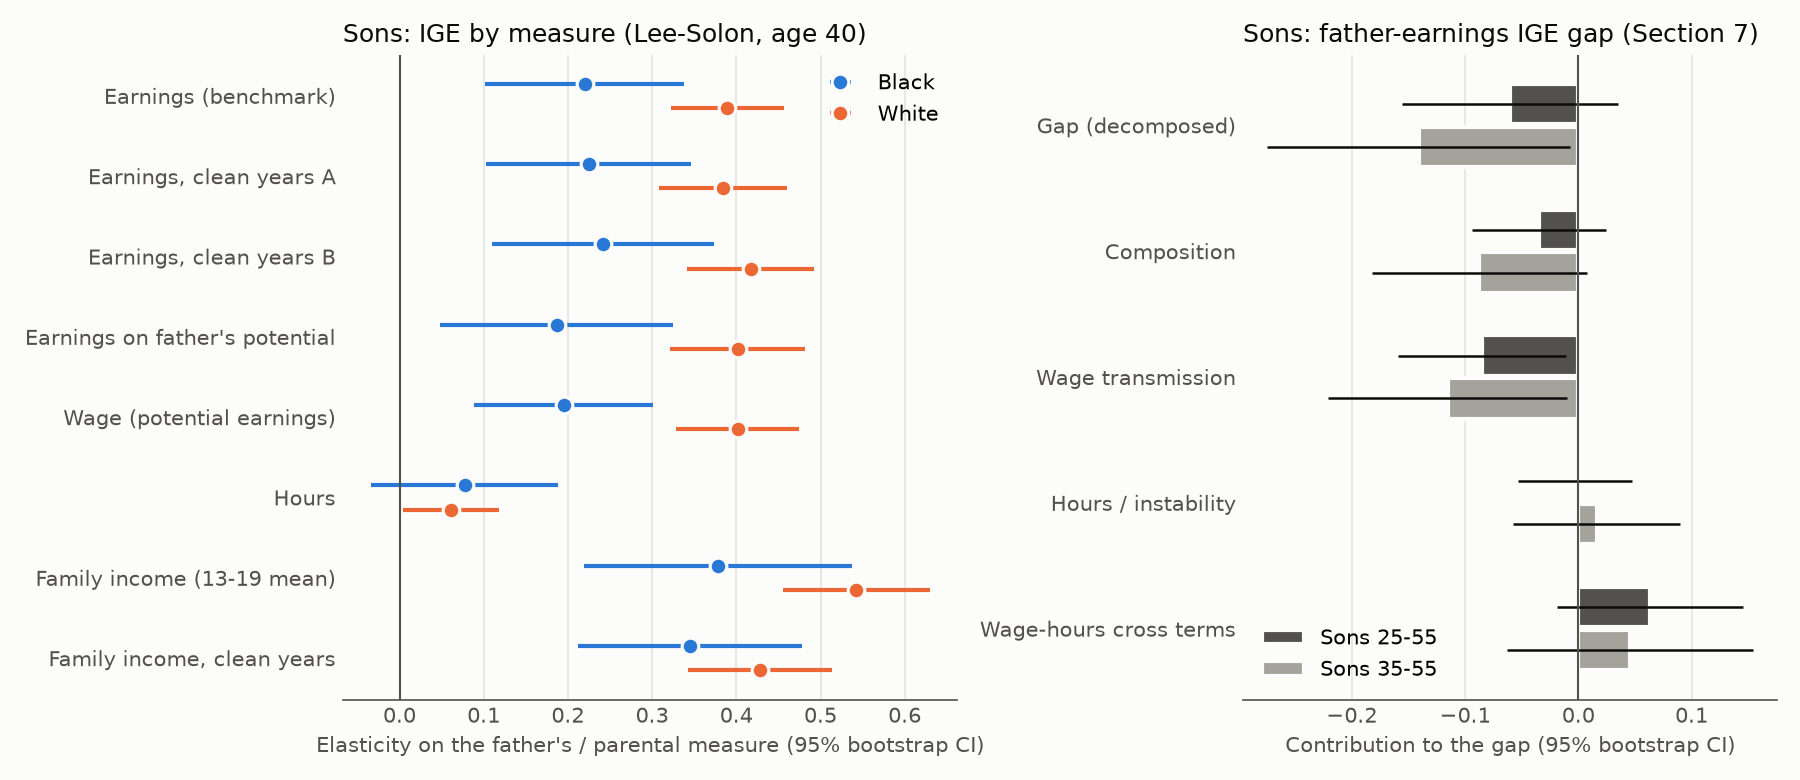
\includegraphics[width=\textwidth]{ige_decomposition.png}
\caption{What the IGE contains: elasticities by measure and the decomposition of the racial gap (PSID, sons)}
\label{fig:decomposition}
\begin{minipage}{\textwidth}\footnotesize \textit{Notes:} Left: elasticities of sons' outcomes with respect to the
father's (or parental) measure, Lee--Solon design at age 40, by race, with 95\% bootstrap confidence intervals; clean
years A exclude displacement and unemployment, B also reduced hours. Right: decomposition of the racial gap (plotted as Black $-$ White in this figure) in
the father-earnings IGE for sons 25--55 and 35--55 (Table~\ref{tab:decomposition}). This figure colours Black
estimates blue and White estimates orange. Code: \texttt{24.IGEDecomposition.py}.\end{minipage}
\end{figure}

\subsection{Designs that were not informative}

\paragraph{Lifetime means.} Averaging each son's earnings over his whole observed career averages the ages before
and after the divergence. In the lifetime-mean design the White--Black gap in the father-earnings IGE is 0.044
(0.050), against 0.169$^{**}$ (0.074) at age 40 in the age-interacted design.\footnote{\texttt{output/ige\_decomposition.md},
Sections 2 and 7. Code: \texttt{24.IGEDecomposition.py}.}

\paragraph{Father's working-life measure.} Measuring the father's earnings over his own working life (25--55) mixes
years after the son has left home; the gap is 0.129 (0.083). The childhood-window measure is the one the question
requires.

\paragraph{Re-weighting ratios and tercile slopes.} Ratios of re-weighted to raw gaps at one age are ratios of noisy
gaps (0.593, s.e.\ 0.653, for the family-income IGE), and IGE slopes within terciles of the parental distribution are
too noisy to be informative (0.802, s.e.\ 0.401, for Black sons in the top tercile). The band-by-band re-weighting and
the comparison below the median of Section~\ref{sec:ageprofile} use the whole profile and are the informative
versions.

\paragraph{Coded occupation changes.} Moves to higher-paying occupations coded from consecutive interviews fall with
parental income ($-0.031^{***}$), because PSID occupations are coded independently in each wave after 1980 and coded
changes contain much churning and coding noise. The level decomposition of Section~\ref{sec:careers} is used
instead.\footnote{\texttt{output/career\_wage\_growth.md}, Section 4. Code: \texttt{27.CareerWageGrowth.py}.}

\paragraph{A fast track inside well-paid cells.} The parental-income gradient of wage growth inside well-paid,
fast-growing cells (0.146$^{**}$) is larger than outside them (0.043), but the difference, 0.103 ($p=0.113$), is
imprecise.

\paragraph{Cleaning daughters' years.} Displacement and unemployment flags exist only for male heads in the PSID, so
daughters' own years cannot be purged of shocks.

\section{Career Evidence: Further Results}\label{app:careers}

\subsection{Industries}

Industry codes of all PSID waves and of the CPS Outgoing Rotation Groups are mapped to the 222 industries of the
ind1990ddx scheme and grouped into 33 industry groups.\footnote{1970 Census codes are bridged to 1980 codes with the
Census Bureau's 1970--1980 table, weighted by the male experienced civilian labor force; 2000 codes use Dorn's weighted
crosswalk; 2002 and 2012 codes use the first three digits. Code: \texttt{IGE/32.IndustryCareers.py}
(\texttt{output/industry\_careers.md}).} For each industry $j$, among men aged 25--64 in the 1992--2002 CPS, I estimate
its wage level at 40, $P_j$, and the slope of its age--wage profile, $B_j$, relative to the average industry
(Table~\ref{tab:industrygroups}). Sons of richer parents sort into better-paid and steeper industries by 25--34
(Table~\ref{tab:industrysorting}). Writing the son's log wage as his industry's level, plus its career slope times his
age, plus a within-industry residual, the career slope accounts for 0.084$^{***}$ of the pooled rise of wage
persistence and 0.051$^{***}$ of the change in the racial gap (Table~\ref{tab:industrydecomp}); with each industry's
full nonlinear profile, 0.118$^{***}$ and 0.074$^{***}$, and with the industry fixed at 25--34, 0.132$^{***}$ and
0.086$^{***}$ (Table~\ref{tab:industrynonlinear}). Same-employer wage growth rises with parental income for White sons
within detailed industries (0.015$^{***}$) and most steeply in high-paying service industries (0.040$^{**}$), and not for
Black sons (Table~\ref{tab:industrygrowth}). Following the father's industry is described in
Table~\ref{tab:fatherindustry}.

\begin{table}[!htbp]
\centering
\caption{Industry wage levels and career slopes (CPS MORG men 25--64, 1992--2002)}
\label{tab:industrygroups}
\resizebox{\ifdim\width>\textwidth\textwidth\else\width\fi}{!}{%
\resizebox*{!}{\ifdim\totalheight>0.85\textheight 0.85\textheight\else\totalheight\fi}{%
\begin{tabular}{lccccc}
\toprule
Industry group & \begin{tabular}[b]{@{}c@{}}Level $P$\\at 40\end{tabular} & \begin{tabular}[b]{@{}c@{}}Career slope $B$\\per 10 years\end{tabular} & \begin{tabular}[b]{@{}c@{}}Raw growth\\25--34 to\\45--55\end{tabular} & \begin{tabular}[b]{@{}c@{}}Return to\\experience\\5 to 25 years\end{tabular} & \begin{tabular}[b]{@{}c@{}}Employment\\share\end{tabular} \\
 & (1) & (2) & (3) & (4) & (5) \\
\midrule
Education & 0.082 & 0.077 & 0.432 & 0.437 & 0.055 \\
Legal services & 0.538 & 0.069 & 0.340 & 0.358 & 0.006 \\
Professional services (engineering, accounting, research, consulting) & 0.394 & 0.039 & 0.314 & 0.380 & 0.024 \\
Manufacturing: chemicals, petroleum, rubber, plastics & 0.115 & 0.038 & 0.314 & 0.340 & 0.029 \\
Other health services & 0.093 & 0.031 & 0.317 & 0.264 & 0.015 \\
Hospitals & 0.071 & 0.029 & 0.314 & 0.485 & 0.022 \\
Communications & 0.254 & 0.022 & 0.297 & 0.412 & 0.018 \\
Manufacturing: motor vehicles, aircraft, other transport eq. & 0.156 & 0.022 & 0.279 & 0.331 & 0.033 \\
Finance: banking, credit, securities & 0.395 & 0.021 & 0.322 & 0.387 & 0.022 \\
Insurance & 0.320 & 0.020 & 0.315 & 0.393 & 0.014 \\
Manufacturing: instruments, misc. manufacturing & 0.097 & 0.020 & 0.301 & 0.337 & 0.014 \\
Manufacturing: textiles, apparel, leather & $-$0.235 & 0.015 & 0.260 & 0.275 & 0.011 \\
Utilities and sanitary services & 0.152 & 0.011 & 0.267 & 0.383 & 0.023 \\
Mining & 0.067 & 0.011 & 0.277 & 0.318 & 0.009 \\
Public administration (incl. postal) & 0.142 & 0.009 & 0.250 & 0.330 & 0.075 \\
Manufacturing: food, tobacco & $-$0.141 & 0.007 & 0.264 & 0.300 & 0.021 \\
Manufacturing: electrical equipment & 0.186 & 0.003 & 0.230 & 0.298 & 0.021 \\
Manufacturing: paper, printing, publishing & 0.034 & 0.002 & 0.229 & 0.333 & 0.026 \\
Computer and data processing services & 0.460 & 0.001 & 0.233 & 0.327 & 0.017 \\
Manufacturing: primary and fabricated metals & $-$0.061 & 0.001 & 0.222 & 0.269 & 0.029 \\
Manufacturing: wood, furniture, stone, glass & $-$0.183 & 0.000 & 0.227 & 0.289 & 0.025 \\
Manufacturing: machinery and computers & 0.105 & $-$0.002 & 0.235 & 0.294 & 0.033 \\
Social services, religious, membership & $-$0.128 & $-$0.006 & 0.260 & 0.236 & 0.019 \\
Wholesale trade & $-$0.008 & $-$0.008 & 0.230 & 0.289 & 0.053 \\
Construction & $-$0.031 & $-$0.010 & 0.205 & 0.282 & 0.096 \\
Transportation (excl. postal) & $-$0.052 & $-$0.019 & 0.195 & 0.278 & 0.058 \\
Eating, drinking, hotels & $-$0.467 & $-$0.023 & 0.207 & 0.311 & 0.039 \\
Retail trade (excl. eating, drinking) & $-$0.177 & $-$0.035 & 0.197 & 0.285 & 0.090 \\
Real estate & $-$0.072 & $-$0.036 & 0.168 & 0.177 & 0.014 \\
Automotive and repair services & $-$0.205 & $-$0.043 & 0.172 & 0.250 & 0.021 \\
Other business services & $-$0.173 & $-$0.043 & 0.183 & 0.228 & 0.029 \\
Personal services, entertainment & $-$0.195 & $-$0.046 & 0.180 & 0.237 & 0.020 \\
Agriculture, forestry, fishing & $-$0.530 & $-$0.064 & 0.100 & 0.177 & 0.019 \\
\bottomrule
\end{tabular}}}
\par\smallskip
\begin{minipage}{\textwidth}\footnotesize \textit{Notes:} Industries harmonised to the ind1990ddx scheme (222 industries, 33 groups). Industry level $P_j$ and career slope $B_j$ from CPS MORG men aged 25--64, 1992--2002 (743,983 observations): relative log wage $= f(\text{age}) + P_j + B_j(\text{age}-40)/10$, both employment-weighted mean zero. Rows sorted by $B$. Raw growth: mean relative log wage at 45--55 minus 25--34. Return to experience: predicted wage growth from 5 to 25 years of potential experience with years of schooling held fixed. Industry averages; the composition of workers is not held fixed. Across men, the standard deviation of $P$ is 0.232 and of $B$ 0.037. Source: \texttt{IGE/32.IndustryCareers.py} (\texttt{output/industry\_careers.csv}); table built by \texttt{IGE/28.PaperBTables.py}.\end{minipage}
\end{table}

\begin{table}[!htbp]
\centering
\caption{Sorting into industries by parental income (PSID, sons)}
\label{tab:industrysorting}
\resizebox{\ifdim\width>\textwidth\textwidth\else\width\fi}{!}{%
\resizebox*{!}{\ifdim\totalheight>0.85\textheight 0.85\textheight\else\totalheight\fi}{%
\begin{tabular}{lccccccc}
\toprule
Panel / row & \begin{tabular}[b]{@{}c@{}}Industry\\level $P$\end{tabular} & \begin{tabular}[b]{@{}c@{}}Industry\\slope $B$\end{tabular} & \begin{tabular}[b]{@{}c@{}}Finance,\\insurance,\\real estate\end{tabular} & \begin{tabular}[b]{@{}c@{}}Legal,\\professional\\services\end{tabular} & \begin{tabular}[b]{@{}c@{}}Computer,\\business\\services\end{tabular} & \begin{tabular}[b]{@{}c@{}}Steep-slope\\industry\end{tabular} & \begin{tabular}[b]{@{}c@{}}High-premium\\industry\end{tabular} \\
 & (1) & (2) & (3) & (4) & (5) & (6) & (7) \\
\midrule
\multicolumn{8}{l}{\textit{Pooled (weighted)}} \\
ln parental income, sons 25--34 & $0.077^{***}$ & $0.010^{***}$ & $0.036^{***}$ & $0.034^{***}$ & $0.022^{***}$ & $0.087^{***}$ & $0.085^{***}$ \\
 & (0.009) & (0.001) & (0.007) & (0.005) & (0.006) & (0.013) & (0.014) \\
\quad Mean of outcome, 25--34 & $-$0.007 & $-$0.002 & 0.049 & 0.038 & 0.052 & 0.257 & 0.239 \\
ln parental income, sons 35--55 & $0.075^{***}$ & $0.009^{***}$ & $0.037^{***}$ & $0.034^{***}$ & $0.023^{***}$ & $0.081^{***}$ & $0.082^{***}$ \\
 & (0.011) & (0.002) & (0.010) & (0.007) & (0.009) & (0.019) & (0.019) \\
\quad Mean of outcome, 35--55 & 0.021 & 0.001 & 0.054 & 0.041 & 0.057 & 0.293 & 0.265 \\
Change, (35--55) $-$ (25--34) & $-0.002$ & $-0.001$ & $0.001$ & $0.000$ & $0.001$ & $-0.006$ & $-0.003$ \\
 & (0.007) & (0.001) & (0.008) & (0.006) & (0.008) & (0.015) & (0.013) \\
\addlinespace
\multicolumn{8}{l}{\textit{Black}} \\
ln parental income, sons 25--34 & $0.044^{***}$ & $0.005^{***}$ & $0.017^{***}$ & $0.008^{***}$ & $0.008$ & $0.062^{***}$ & $0.052^{***}$ \\
 & (0.008) & (0.001) & (0.007) & (0.003) & (0.007) & (0.016) & (0.015) \\
\quad Mean of outcome, 25--34 & $-$0.062 & $-$0.007 & 0.039 & 0.010 & 0.048 & 0.222 & 0.199 \\
ln parental income, sons 35--55 & $0.042^{***}$ & $0.003^{*}$ & $0.015^{**}$ & $0.004$ & $0.011$ & $0.046^{**}$ & $0.060^{***}$ \\
 & (0.010) & (0.002) & (0.007) & (0.004) & (0.008) & (0.022) & (0.021) \\
\quad Mean of outcome, 35--55 & $-$0.042 & $-$0.006 & 0.036 & 0.013 & 0.045 & 0.227 & 0.215 \\
Change, (35--55) $-$ (25--34) & $-0.002$ & $-0.002$ & $-0.002$ & $-0.004$ & $0.003$ & $-0.016$ & $0.008$ \\
 & (0.009) & (0.002) & (0.006) & (0.005) & (0.009) & (0.019) & (0.018) \\
\addlinespace
\multicolumn{8}{l}{\textit{White}} \\
ln parental income, sons 25--34 & $0.082^{***}$ & $0.010^{***}$ & $0.041^{***}$ & $0.037^{***}$ & $0.030^{***}$ & $0.103^{***}$ & $0.101^{***}$ \\
 & (0.010) & (0.001) & (0.008) & (0.006) & (0.006) & (0.015) & (0.015) \\
\quad Mean of outcome, 25--34 & $-$0.009 & $-$0.002 & 0.048 & 0.039 & 0.048 & 0.249 & 0.235 \\
ln parental income, sons 35--55 & $0.084^{***}$ & $0.009^{***}$ & $0.048^{***}$ & $0.040^{***}$ & $0.036^{***}$ & $0.092^{***}$ & $0.100^{***}$ \\
 & (0.013) & (0.002) & (0.012) & (0.009) & (0.009) & (0.021) & (0.020) \\
\quad Mean of outcome, 35--55 & 0.022 & 0.001 & 0.053 & 0.043 & 0.053 & 0.292 & 0.265 \\
Change, (35--55) $-$ (25--34) & $0.003$ & $-0.001$ & $0.007$ & $0.003$ & $0.006$ & $-0.011$ & $-0.001$ \\
 & (0.008) & (0.001) & (0.009) & (0.007) & (0.008) & (0.017) & (0.015) \\
\addlinespace
\multicolumn{8}{l}{\textit{White $-$ Black}} \\
ln parental income, sons 25--34 & $0.038^{***}$ & $0.005^{***}$ & $0.024^{**}$ & $0.029^{***}$ & $0.022^{**}$ & $0.040^{*}$ & $0.048^{**}$ \\
 & (0.013) & (0.002) & (0.010) & (0.007) & (0.009) & (0.022) & (0.021) \\
ln parental income, sons 35--55 & $0.043^{**}$ & $0.006^{**}$ & $0.032^{**}$ & $0.036^{***}$ & $0.025^{**}$ & $0.045$ & $0.040$ \\
 & (0.017) & (0.003) & (0.014) & (0.009) & (0.012) & (0.030) & (0.029) \\
Change, (35--55) $-$ (25--34) & $0.005$ & $0.001$ & $0.008$ & $0.007$ & $0.003$ & $0.005$ & $-0.008$ \\
 & (0.012) & (0.002) & (0.011) & (0.008) & (0.012) & (0.026) & (0.023) \\
\bottomrule
\end{tabular}}}
\par\smallskip
\begin{minipage}{\textwidth}\footnotesize \textit{Notes:} Son-year regressions of the outcome in the header on log parental income with the controls of Table~\ref{tab:industrydecomp}; columns (3)--(7) are linear probability models. Industries harmonised to the ind1990ddx scheme (222 industries, 33 groups). Industry level $P_j$ and career slope $B_j$ from CPS MORG men aged 25--64, 1992--2002 (743,983 observations): relative log wage $= f(\text{age}) + P_j + B_j(\text{age}-40)/10$, both employment-weighted mean zero. Steep-slope and high-premium industries: top quartile of men's employment by $B_j$ and by $P_j$ (Table~\ref{tab:industrygroups}). Standard errors clustered by 1968 family. Pooled: weighted; Black and White: unweighted. $^{***}$ $p<0.01$, $^{**}$ $p<0.05$, $^{*}$ $p<0.1$. Source: \texttt{32.IndustryCareers.py} (\texttt{output/industry\_careers.csv}); table built by \texttt{28.PaperBTables.py}.\end{minipage}
\end{table}

\begin{table}[!htbp]
\centering
\caption{Wage persistence by age: industry level, industry career slope and within industry (PSID, sons)}
\label{tab:industrydecomp}
\resizebox{\ifdim\width>\textwidth\textwidth\else\width\fi}{!}{%
\resizebox*{!}{\ifdim\totalheight>0.85\textheight 0.85\textheight\else\totalheight\fi}{%
\begin{tabular}{lccccccccc}
\toprule
Panel / row & \begin{tabular}[b]{@{}c@{}}ln wage\end{tabular} & \begin{tabular}[b]{@{}c@{}}Industry\\level $P$\end{tabular} & \begin{tabular}[b]{@{}c@{}}Industry\\career slope\\$B\times t$\end{tabular} & \begin{tabular}[b]{@{}c@{}}Within-\\industry\\residual\end{tabular} & \begin{tabular}[b]{@{}c@{}}Occupation\\score\end{tabular} & \begin{tabular}[b]{@{}c@{}}Joint:\\occupation\end{tabular} & \begin{tabular}[b]{@{}c@{}}Joint:\\industry level\\net of occ.\end{tabular} & \begin{tabular}[b]{@{}c@{}}Joint:\\industry slope\\net of occ.\end{tabular} & \begin{tabular}[b]{@{}c@{}}Joint:\\residual\end{tabular} \\
 & (1) & (2) & (3) & (4) & (5) & (6) & (7) & (8) & (9) \\
\midrule
\multicolumn{10}{l}{\textit{Pooled (weighted): coefficient on log parental income}} \\
Sons aged 25--34 & $0.256^{***}$ & $0.077^{***}$ & $-0.010^{***}$ & $0.190^{***}$ & $0.159^{***}$ & $0.141^{***}$ & $0.025^{***}$ & $-0.011^{***}$ & $0.101^{***}$ \\
 & (0.017) & (0.009) & (0.001) & (0.015) & (0.010) & (0.008) & (0.004) & (0.001) & (0.014) \\
Sons aged 35--55 & $0.412^{***}$ & $0.075^{***}$ & $0.003^{***}$ & $0.335^{***}$ & $0.173^{***}$ & $0.155^{***}$ & $0.021^{***}$ & $0.003^{***}$ & $0.233^{***}$ \\
 & (0.028) & (0.011) & (0.001) & (0.024) & (0.013) & (0.010) & (0.005) & (0.001) & (0.022) \\
\addlinespace
\multicolumn{10}{l}{\textit{Black: coefficient on log parental income}} \\
Sons aged 25--34 & $0.148^{***}$ & $0.044^{***}$ & $-0.005^{***}$ & $0.109^{***}$ & $0.071^{***}$ & $0.060^{***}$ & $0.013^{***}$ & $-0.006^{***}$ & $0.081^{***}$ \\
 & (0.021) & (0.008) & (0.001) & (0.018) & (0.011) & (0.009) & (0.005) & (0.001) & (0.017) \\
Sons aged 35--55 & $0.157^{***}$ & $0.042^{***}$ & $-0.001$ & $0.116^{***}$ & $0.053^{***}$ & $0.044^{***}$ & $0.015^{***}$ & $0.000$ & $0.098^{***}$ \\
 & (0.031) & (0.010) & (0.001) & (0.027) & (0.014) & (0.012) & (0.005) & (0.001) & (0.023) \\
\addlinespace
\multicolumn{10}{l}{\textit{White: coefficient on log parental income}} \\
Sons aged 25--34 & $0.241^{***}$ & $0.082^{***}$ & $-0.011^{***}$ & $0.170^{***}$ & $0.157^{***}$ & $0.141^{***}$ & $0.024^{***}$ & $-0.013^{***}$ & $0.089^{***}$ \\
 & (0.020) & (0.010) & (0.001) & (0.017) & (0.012) & (0.010) & (0.005) & (0.001) & (0.016) \\
Sons aged 35--55 & $0.419^{***}$ & $0.084^{***}$ & $0.002^{***}$ & $0.332^{***}$ & $0.170^{***}$ & $0.154^{***}$ & $0.022^{***}$ & $0.002^{***}$ & $0.241^{***}$ \\
 & (0.034) & (0.013) & (0.001) & (0.028) & (0.015) & (0.012) & (0.006) & (0.001) & (0.025) \\
\addlinespace
\multicolumn{10}{l}{\textit{White $-$ Black: coefficient on log parental income}} \\
Sons aged 25--34 & $0.093^{***}$ & $0.038^{***}$ & $-0.006^{***}$ & $0.061^{**}$ & $0.087^{***}$ & $0.081^{***}$ & $0.010$ & $-0.007^{***}$ & $0.008$ \\
 & (0.029) & (0.013) & (0.002) & (0.025) & (0.016) & (0.013) & (0.007) & (0.002) & (0.023) \\
Sons aged 35--55 & $0.262^{***}$ & $0.043^{**}$ & $0.003^{***}$ & $0.217^{***}$ & $0.117^{***}$ & $0.110^{***}$ & $0.007$ & $0.003^{***}$ & $0.143^{***}$ \\
 & (0.046) & (0.017) & (0.001) & (0.039) & (0.020) & (0.017) & (0.008) & (0.001) & (0.035) \\
\addlinespace
\multicolumn{10}{l}{\textit{Change in the coefficient, (35--55) $-$ (25--34)}} \\
Pooled (weighted) & $0.156^{***}$ & $-0.002$ & $0.013^{***}$ & $0.145^{***}$ & $0.014$ & $0.015^{*}$ & $-0.004$ & $0.014^{***}$ & $0.132^{***}$ \\
 & (0.024) & (0.007) & (0.002) & (0.022) & (0.010) & (0.009) & (0.004) & (0.002) & (0.021) \\
Black & $0.009$ & $-0.002$ & $0.005^{***}$ & $0.006$ & $-0.018$ & $-0.016^{*}$ & $0.002$ & $0.006^{***}$ & $0.017$ \\
 & (0.026) & (0.009) & (0.002) & (0.025) & (0.011) & (0.010) & (0.005) & (0.002) & (0.022) \\
White & $0.178^{***}$ & $0.003$ & $0.013^{***}$ & $0.162^{***}$ & $0.012$ & $0.014$ & $-0.002$ & $0.015^{***}$ & $0.152^{***}$ \\
 & (0.027) & (0.008) & (0.002) & (0.025) & (0.012) & (0.010) & (0.004) & (0.002) & (0.023) \\
White $-$ Black & $0.170^{***}$ & $0.005$ & $0.009^{***}$ & $0.156^{***}$ & $0.030^{*}$ & $0.029^{**}$ & $-0.004$ & $0.009^{***}$ & $0.135^{***}$ \\
 & (0.038) & (0.012) & (0.002) & (0.035) & (0.017) & (0.014) & (0.007) & (0.002) & (0.032) \\
\addlinespace
\multicolumn{10}{l}{\textit{Share of the change in column (1)}} \\
Pooled change &  & $-0.010$ & $0.084^{***}$ & $0.926^{***}$ & $0.092$ & $0.095^{*}$ & $-0.026$ & $0.087^{***}$ & $0.844^{***}$ \\
 &  & (0.047) & (0.014) & (0.044) & (0.062) & (0.052) & (0.027) & (0.014) & (0.060) \\
White $-$ Black change &  & $0.030$ & $0.051^{***}$ & $0.919^{***}$ & $0.179^{**}$ & $0.173^{**}$ & $-0.021$ & $0.054^{***}$ & $0.794^{***}$ \\
 &  & (0.071) & (0.016) & (0.070) & (0.087) & (0.074) & (0.041) & (0.016) & (0.084) \\
\bottomrule
\end{tabular}}}
\par\smallskip
\begin{minipage}{\textwidth}\footnotesize \textit{Notes:} One regression per cell: the son's outcome (column header) on log parental income, son-years in the age band, controls for quartics in the father's age at 16 and the son's age. Industries harmonised to the ind1990ddx scheme (222 industries, 33 groups). Industry level $P_j$ and career slope $B_j$ from CPS MORG men aged 25--64, 1992--2002 (743,983 observations): relative log wage $= f(\text{age}) + P_j + B_j(\text{age}-40)/10$, both employment-weighted mean zero. Log wage $=P_j+B_j t+$ within-industry residual, so columns (2)--(4) add up to column (1); column (5) is the occupation score of Table~\ref{tab:careerdecomp} on the same son-years; columns (6)--(9) split the log wage with occupation fixed effects and industry levels and slopes estimated jointly, so (7)$+$(8) is what industry adds beyond occupation. Same sample in every column: 1,822 Black sons (12,576 son-years) and 2,639 White sons (25,248). All cells are one stacked system (standard errors clustered by 1968 family); shares by the delta method. Pooled: weighted; Black and White: unweighted. Sign convention: White $-$ Black. Sons select into industries, so the split is accounting, not causal. $^{***}$ $p<0.01$, $^{**}$ $p<0.05$, $^{*}$ $p<0.1$. Source: \texttt{32.IndustryCareers.py} (\texttt{output/industry\_careers.csv}); table built by \texttt{28.PaperBTables.py}.\end{minipage}
\end{table}

\begin{table}[!htbp]
\centering
\caption{Industry and occupation $\times$ industry career profiles: linear and nonlinear (PSID, sons)}
\label{tab:industrynonlinear}
\resizebox{\ifdim\width>\textwidth\textwidth\else\width\fi}{!}{%
\resizebox*{!}{\ifdim\totalheight>0.85\textheight 0.85\textheight\else\totalheight\fi}{%
\begin{tabular}{lcccc}
\toprule
Piece of the log wage & \begin{tabular}[b]{@{}c@{}}Pooled\\change\end{tabular} & \begin{tabular}[b]{@{}c@{}}Share of\\pooled rise\end{tabular} & \begin{tabular}[b]{@{}c@{}}Change of\\White $-$ Black\\gap\end{tabular} & \begin{tabular}[b]{@{}c@{}}Share of\\gap change\end{tabular} \\
 & (1) & (2) & (3) & (4) \\
\midrule
\multicolumn{5}{l}{\textit{A. Sample of Table~\ref{tab:industrydecomp}}} \\
Log wage (total) & $0.155^{***}$ &  & $0.170^{***}$ &  \\
 & (0.024) &  & (0.038) &  \\
Current industry: linear slope $B_j t$ & $0.013^{***}$ & $0.084^{***}$ & $0.009^{***}$ & $0.050^{***}$ \\
 & (0.002) & (0.014) & (0.002) & (0.016) \\
Current industry: age-band profile & $0.018^{***}$ & $0.118^{***}$ & $0.013^{***}$ & $0.074^{***}$ \\
 & (0.002) & (0.020) & (0.003) & (0.023) \\
Current industry: piecewise profile (knots 30/35/45) & $0.018^{***}$ & $0.117^{***}$ & $0.012^{***}$ & $0.072^{***}$ \\
 & (0.002) & (0.019) & (0.003) & (0.023) \\
\addlinespace
\multicolumn{5}{l}{\textit{B. Sons with an industry and cell at 25--34}} \\
Log wage (total) & $0.146^{***}$ &  & $0.159^{***}$ &  \\
 & (0.024) &  & (0.039) &  \\
Industry at 25--34: linear slope & $0.014^{***}$ & $0.093^{***}$ & $0.009^{***}$ & $0.058^{***}$ \\
 & (0.002) & (0.017) & (0.003) & (0.022) \\
Industry at 25--34: age-band profile & $0.019^{***}$ & $0.132^{***}$ & $0.014^{***}$ & $0.086^{***}$ \\
 & (0.003) & (0.024) & (0.004) & (0.032) \\
Current occupation $\times$ industry cell: age-band profile & $0.036^{***}$ & $0.246^{***}$ & $0.022^{***}$ & $0.138^{***}$ \\
 & (0.003) & (0.038) & (0.004) & (0.035) \\
Current occupation group only: age-band profile & $0.031^{***}$ & $0.215^{***}$ & $0.021^{***}$ & $0.131^{***}$ \\
 & (0.002) & (0.034) & (0.003) & (0.032) \\
\quad What industry adds within the current cell & $0.005^{***}$ & $0.031^{***}$ & $0.001$ & $0.007$ \\
 & (0.001) & (0.010) & (0.002) & (0.015) \\
Cell at 25--34: age-band profile & $0.039^{***}$ & $0.267^{***}$ & $0.024^{***}$ & $0.148^{***}$ \\
 & (0.003) & (0.043) & (0.005) & (0.042) \\
Occupation group at 25--34 only: age-band profile & $0.033^{***}$ & $0.222^{***}$ & $0.019^{***}$ & $0.120^{***}$ \\
 & (0.003) & (0.036) & (0.004) & (0.033) \\
\quad What industry adds within the cell at 25--34 & $0.007^{***}$ & $0.045^{***}$ & $0.004$ & $0.028$ \\
 & (0.002) & (0.014) & (0.003) & (0.019) \\
\bottomrule
\end{tabular}}}
\par\smallskip
\begin{minipage}{\textwidth}\footnotesize \textit{Notes:} Each row is a piece of the son's log wage regressed on log parental income by age band (stacked, controls as in Table~\ref{tab:industrydecomp}); columns (1) and (3) give the change of the coefficient from 25--34 to 35--55, pooled and for the White $-$ Black gap, and columns (2) and (4) its share of the change for the log wage. Linear: $B_j t$ as in Table~\ref{tab:industrydecomp}. Age-band profile: the CPS MORG relative wage of the son's industry or cell in his five-year age band, around its age-weighted level (men 25--64, 1992--2002). Cells: 11 occupation groups $\times$ 33 industry groups (267 cells with at least 200 men; smaller cells take their occupation group's profile). `At 25--34': the son's modal industry or cell at 25--34, evaluated at his current age. Standard errors clustered by 1968 family; shares by the delta method. Pooled: weighted. $^{***}$ $p<0.01$, $^{**}$ $p<0.05$, $^{*}$ $p<0.1$. Source: \texttt{IGE/35.EarlyIndustryLatePayoff.py} (\texttt{output/early\_industry\_late\_payoff.csv}); table built by \texttt{IGE/28.PaperBTables.py}.\end{minipage}
\end{table}

\begin{table}[!htbp]
\centering
\caption{Wage growth with the same employer by parental income, within industries (PSID, sons)}
\label{tab:industrygrowth}
\resizebox{\ifdim\width>\textwidth\textwidth\else\width\fi}{!}{%
\resizebox*{!}{\ifdim\totalheight>0.85\textheight 0.85\textheight\else\totalheight\fi}{%
\begin{tabular}{lcccccc}
\toprule
Panel / row & \begin{tabular}[b]{@{}c@{}}All\\industries\end{tabular} & \begin{tabular}[b]{@{}c@{}}+ industry-\\group FE\end{tabular} & \begin{tabular}[b]{@{}c@{}}+ fine-\\industry FE\end{tabular} & \begin{tabular}[b]{@{}c@{}}Finance, legal,\\professional,\\business\end{tabular} & \begin{tabular}[b]{@{}c@{}}Other\\steep-slope\\industries\end{tabular} & \begin{tabular}[b]{@{}c@{}}All other\\industries\end{tabular} \\
 & (1) & (2) & (3) & (4) & (5) & (6) \\
\midrule
\multicolumn{7}{l}{\textit{Pooled (weighted)}} \\
ln parental income, sons 25--34 & $0.012^{**}$ & $0.007$ & $0.005$ & $0.024$ & $0.021$ & $0.000$ \\
 & (0.005) & (0.006) & (0.006) & (0.021) & (0.014) & (0.006) \\
\quad Stayer pairs, 25--34 & 9,365 & 9,365 & 9,365 & 1,121 & 1,834 & 6,410 \\
ln parental income, sons 35--55 & $0.001$ & $-0.002$ & $-0.002$ & $-0.001$ & $0.000$ & $-0.002$ \\
 & (0.003) & (0.003) & (0.003) & (0.010) & (0.005) & (0.004) \\
\quad Stayer pairs, 35--55 & 12,246 & 12,246 & 12,246 & 1,416 & 2,869 & 7,961 \\
\addlinespace
\multicolumn{7}{l}{\textit{Black}} \\
ln parental income, sons 25--34 & $0.003$ & $0.002$ & $0.002$ &  & $0.018$ & $0.001$ \\
 & (0.008) & (0.008) & (0.009) &  & (0.020) & (0.010) \\
\quad Stayer pairs, 25--34 & 2,947 & 2,947 & 2,947 &  & 610 & 2,100 \\
ln parental income, sons 35--55 & $0.000$ & $0.001$ & $0.002$ & $0.030$ & $0.018^{*}$ & $-0.009$ \\
 & (0.004) & (0.004) & (0.005) & (0.024) & (0.010) & (0.006) \\
\quad Stayer pairs, 35--55 & 3,864 & 3,864 & 3,864 & 309 & 857 & 2,698 \\
\addlinespace
\multicolumn{7}{l}{\textit{White}} \\
ln parental income, sons 25--34 & $0.021^{***}$ & $0.015^{***}$ & $0.015^{***}$ & $0.040^{**}$ & $0.026$ & $0.009$ \\
 & (0.006) & (0.006) & (0.006) & (0.017) & (0.019) & (0.006) \\
\quad Stayer pairs, 25--34 & 6,427 & 6,427 & 6,427 & 884 & 1,224 & 4,319 \\
ln parental income, sons 35--55 & $0.001$ & $-0.002$ & $-0.003$ & $0.004$ & $-0.008$ & $0.000$ \\
 & (0.004) & (0.004) & (0.004) & (0.012) & (0.007) & (0.005) \\
\quad Stayer pairs, 35--55 & 8,383 & 8,383 & 8,383 & 1,107 & 2,012 & 5,264 \\
\addlinespace
\multicolumn{7}{l}{\textit{White $-$ Black}} \\
ln parental income, sons 25--34 & $0.018^{*}$ & $0.013$ & $0.014$ &  & $0.008$ & $0.008$ \\
 & (0.010) & (0.010) & (0.011) &  & (0.027) & (0.011) \\
ln parental income, sons 35--55 & $0.001$ & $-0.003$ & $-0.005$ & $-0.026$ & $-0.025^{**}$ & $0.009$ \\
 & (0.006) & (0.006) & (0.007) & (0.027) & (0.012) & (0.008) \\
\bottomrule
\end{tabular}}}
\par\smallskip
\begin{minipage}{\textwidth}\footnotesize \textit{Notes:} Outcome in every column: annualised log-wage growth between consecutive interviews 1--2 years apart (waves 1985--2023) for sons who stayed with their employer. Columns (2)--(3) add fixed effects for the industry of the later interview, so they compare sons in the same industry; columns (4)--(6) split the sample by the son's industry. Controls: quartic in age, year fixed effects. Cells with fewer than 250 pairs are left blank. Standard errors clustered by 1968 family. $^{***}$ $p<0.01$, $^{**}$ $p<0.05$, $^{*}$ $p<0.1$. Source: \texttt{32.IndustryCareers.py} (\texttt{output/industry\_careers.csv}); table built by \texttt{28.PaperBTables.py}.\end{minipage}
\end{table}

\begin{table}[!htbp]
\centering
\caption{Following the father into his industry: how often and does it pay (PSID, sons)}
\label{tab:fatherindustry}
\resizebox{\ifdim\width>\textwidth\textwidth\else\width\fi}{!}{%
\resizebox*{!}{\ifdim\totalheight>0.85\textheight 0.85\textheight\else\totalheight\fi}{%
\begin{tabular}{lccccccc}
\toprule
Panel / row & \begin{tabular}[b]{@{}c@{}}Son in\\finance,\\insurance,\\real estate\end{tabular} & \begin{tabular}[b]{@{}c@{}}Son in\\legal,\\professional\end{tabular} & \begin{tabular}[b]{@{}c@{}}ln wage,\\25--34\end{tabular} & \begin{tabular}[b]{@{}c@{}}ln wage,\\35--55\end{tabular} & \begin{tabular}[b]{@{}c@{}}Annual\\wage growth,\\30--55\end{tabular} & \begin{tabular}[b]{@{}c@{}}Same-employer\\wage growth,\\30--55\end{tabular} & \begin{tabular}[b]{@{}c@{}}ln wage,\\person FE\end{tabular} \\
 & (1) & (2) & (3) & (4) & (5) & (6) & (7) \\
\midrule
\multicolumn{8}{l}{\textit{Pooled (weighted)}} \\
Father worked in the same industry set & $0.108^{**}$ & $0.072^{*}$ &  &  &  &  &  \\
 & (0.047) & (0.040) &  &  &  &  &  \\
Son in the father's industry group &  &  & $0.079^{***}$ & $0.054^{*}$ & $0.005$ & $-0.006$ & $0.039$ \\
 &  &  & (0.023) & (0.030) & (0.005) & (0.005) & (0.025) \\
Tenure (per 10 years) $\times$ in father's industry &  &  &  &  &  &  & $-0.042^{**}$ \\
 &  &  &  &  &  &  & (0.020) \\
\addlinespace
\multicolumn{8}{l}{\textit{Black}} \\
Father worked in the same industry set & $-0.003$ & $-0.012^{***}$ &  &  &  &  &  \\
 & (0.023) & (0.004) &  &  &  &  &  \\
Son in the father's industry group &  &  & $0.034$ & $0.088$ & $0.000$ & $-0.021^{**}$ & $0.115^{***}$ \\
 &  &  & (0.042) & (0.073) & (0.010) & (0.010) & (0.040) \\
Tenure (per 10 years) $\times$ in father's industry &  &  &  &  &  &  & $-0.068^{*}$ \\
 &  &  &  &  &  &  & (0.039) \\
\addlinespace
\multicolumn{8}{l}{\textit{White}} \\
Father worked in the same industry set & $0.122^{***}$ & $0.067^{*}$ &  &  &  &  &  \\
 & (0.047) & (0.040) &  &  &  &  &  \\
Son in the father's industry group &  &  & $0.057^{**}$ & $0.046$ & $0.006$ & $-0.004$ & $0.024$ \\
 &  &  & (0.023) & (0.029) & (0.006) & (0.005) & (0.022) \\
Tenure (per 10 years) $\times$ in father's industry &  &  &  &  &  &  & $-0.040^{**}$ \\
 &  &  &  &  &  &  & (0.019) \\
\addlinespace
\multicolumn{8}{l}{\textit{White $-$ Black}} \\
Father worked in the same industry set & $0.125^{**}$ & $0.079^{*}$ &  &  &  &  &  \\
 & (0.052) & (0.041) &  &  &  &  &  \\
Son in the father's industry group &  &  & $0.023$ & $-0.041$ & $0.006$ & $0.016$ &  \\
 &  &  & (0.048) & (0.078) & (0.012) & (0.012) &  \\
Tenure (per 10 years) $\times$ in father's industry &  &  &  &  &  &  & $0.028$ \\
 &  &  &  &  &  &  & (0.043) \\
\bottomrule
\end{tabular}}}
\par\smallskip
\begin{minipage}{\textwidth}\footnotesize \textit{Notes:} Father: male head of the son's family at 16; his industry is the modal code over his years as head when the son was 12--18 (father-present sons: 52\% of Black and 87\% of White sons). The PSID has no employer identifiers, so following is measured at the industry level. Columns (1)--(2): son-years 25--55, linear probability that the son works in the industry set, on an indicator that the father did and log parental income. Columns (3)--(6): son-year regressions on an indicator that the son works in his father's industry group (33 groups), holding log parental income, years of education and the level $P_j$ and slope $B_j$ of the son's industry fixed; growth between consecutive interviews 1--2 years apart. Column (7): within-son regression on tenure, its square, tenure $\times$ following, following and tenure $\times$ log parental income, with a quartic in age and year fixed effects. Standard errors clustered by 1968 family. Pooled: weighted. Only 21 Black sons had a father in finance, insurance or real estate and 8 in legal or professional services. Sons who follow may differ in unobserved ways; descriptive. $^{***}$ $p<0.01$, $^{**}$ $p<0.05$, $^{*}$ $p<0.1$. Source: \texttt{32.IndustryCareers.py} (\texttt{output/industry\_careers.csv}); table built by \texttt{28.PaperBTables.py}.\end{minipage}
\end{table}


\subsection{Growth, tenure, promotion and displacement}

Table~\ref{tab:careergrowth} splits annual wage growth into occupational-score and residual growth with the same and a
new employer; Table~\ref{tab:tenure} reports wage--tenure profiles within sons, which steepen with parental income for
White sons (0.068$^{***}$ per ten years of tenure and log point of parental income) and not for Black sons (0.013).
Tables~\ref{tab:promotion} and \ref{tab:hegde} report entry into supervisory and managerial occupations and the
analogue to \citet{hegde2026racial}: the after-35 change relative to 25--34 is not significant (triple interaction
0.008, s.e.\ 0.011, for the change of the White $-$ Black difference), and holding the wage and occupation at 28--32 fixed the gradients are 0.014 for White and
$-0.010$ for Black sons. Table~\ref{tab:careerdisp} reports the wage loss after displacement, 0.131$^{***}$, of which
0.028$^{***}$ is a lower occupational score. Table~\ref{tab:mediation} reports the coefficient movements when education
and instability shares are added to the IGE, and Table~\ref{tab:nlsycareer} the NLSY79 version of the occupational
decomposition: the pooled wage gradient rises from 0.252$^{***}$ at 25--34 to 0.381$^{***}$ at 45--55, almost all within
occupations, and the White--Black gap changes by 0.059$^{*}$.

\begin{table}[!htbp]
\centering
\caption{Annual wage growth by parental income: within and across employers (PSID, sons)}
\label{tab:careergrowth}
\resizebox{\ifdim\width>\textwidth\textwidth\else\width\fi}{!}{%
\resizebox*{!}{\ifdim\totalheight>0.85\textheight 0.85\textheight\else\totalheight\fi}{%
\begin{tabular}{lcccccc}
\toprule
Panel / row & \begin{tabular}[b]{@{}c@{}}Annual\\ln wage\\growth\end{tabular} & \begin{tabular}[b]{@{}c@{}}Score growth,\\same\\employer\end{tabular} & \begin{tabular}[b]{@{}c@{}}Residual growth,\\same\\employer\end{tabular} & \begin{tabular}[b]{@{}c@{}}Score growth,\\new\\employer\end{tabular} & \begin{tabular}[b]{@{}c@{}}Residual growth,\\new\\employer\end{tabular} & \begin{tabular}[b]{@{}c@{}}Stayed\\with\\employer\end{tabular} \\
 & (1) & (2) & (3) & (4) & (5) & (6) \\
\midrule
\multicolumn{7}{l}{\textit{Pooled (weighted)}} \\
ln parental income, sons 25--34 & $0.015^{***}$ & $0.001$ & $0.010^{**}$ & $0.002$ & $0.003$ & $0.022^{**}$ \\
 & (0.005) & (0.002) & (0.004) & (0.001) & (0.003) & (0.009) \\
\quad Mean of outcome / pairs, 25--34 & 0.054 & 0.009 & 0.039 & 0.002 & 0.004 & 11,578 pairs \\
ln parental income, sons 35--55 & $0.004$ & $-0.002^{*}$ & $0.003$ & $0.000$ & $0.002$ & $0.020^{**}$ \\
 & (0.003) & (0.001) & (0.003) & (0.001) & (0.002) & (0.008) \\
\quad Mean of outcome / pairs, 35--55 & 0.020 & 0.002 & 0.017 & $-$0.001 & 0.002 & 14,185 pairs \\
\addlinespace
\multicolumn{7}{l}{\textit{Black}} \\
ln parental income, sons 25--34 & $-0.001$ & $0.004$ & $0.000$ & $0.003$ & $-0.008$ & $0.018$ \\
 & (0.006) & (0.003) & (0.007) & (0.002) & (0.005) & (0.013) \\
\quad Mean of outcome / pairs, 25--34 & 0.042 & 0.003 & 0.040 & 0.001 & $-$0.003 & 3,725 pairs \\
ln parental income, sons 35--55 & $-0.002$ & $-0.001$ & $0.001$ & $-0.001$ & $-0.001$ & $-0.011$ \\
 & (0.004) & (0.002) & (0.004) & (0.001) & (0.003) & (0.012) \\
\quad Mean of outcome / pairs, 35--55 & 0.015 & 0.003 & 0.013 & 0.000 & $-$0.002 & 4,537 pairs \\
\addlinespace
\multicolumn{7}{l}{\textit{White}} \\
ln parental income, sons 25--34 & $0.020^{***}$ & $0.000$ & $0.018^{***}$ & $0.001$ & $0.001$ & $0.020^{**}$ \\
 & (0.005) & (0.002) & (0.005) & (0.001) & (0.003) & (0.010) \\
\quad Mean of outcome / pairs, 25--34 & 0.054 & 0.010 & 0.038 & 0.002 & 0.005 & 7,862 pairs \\
ln parental income, sons 35--55 & $0.007^{**}$ & $-0.001$ & $0.003$ & $0.001$ & $0.004^{**}$ & $0.025^{***}$ \\
 & (0.003) & (0.001) & (0.004) & (0.001) & (0.002) & (0.009) \\
\quad Mean of outcome / pairs, 35--55 & 0.021 & 0.002 & 0.018 & $-$0.001 & 0.002 & 9,649 pairs \\
\addlinespace
\multicolumn{7}{l}{\textit{White $-$ Black}} \\
ln parental income, sons 25--34 & $0.021^{***}$ & $-0.003$ & $0.018^{**}$ & $-0.002$ & $0.009$ & $0.001$ \\
 & (0.008) & (0.004) & (0.008) & (0.003) & (0.006) & (0.016) \\
ln parental income, sons 35--55 & $0.009^{*}$ & $0.000$ & $0.002$ & $0.002$ & $0.005$ & $0.036^{**}$ \\
 & (0.005) & (0.002) & (0.005) & (0.001) & (0.004) & (0.015) \\
\bottomrule
\end{tabular}}}
\par\smallskip
\begin{minipage}{\textwidth}\footnotesize \textit{Notes:} Consecutive interviews 1--2 years apart (waves 1985--2023) with a valid wage, a mapped occupation and tenure with the present employer. Annualised log-wage growth = score growth + residual growth, each split by whether the son stayed with the same employer; columns (2)--(5) add up to column (1). Column (6): share of stayers (linear probability). Controls: quartic in age and year fixed effects. Mean row: mean of the outcome in columns (1)--(5) and the number of son-year pairs. Coding noise in occupations inflates score changes in both directions. Standard errors clustered by 1968 family. Occupational wage score: mean log hourly wage of men aged 25--64 in the occupation relative to all men (CPS MORG, base 1992--2002), occupations harmonised to Dorn's occ1990dd scheme; log wage = score (between occupations) + residual (within occupation), so the score and residual columns add up to the log-wage column on the same sample. $^{***}$ $p<0.01$, $^{**}$ $p<0.05$, $^{*}$ $p<0.1$. Source: \texttt{IGE/27.CareerWageGrowth.py} (\texttt{output/career\_wage\_growth.csv}); table built by \texttt{IGE/28.PaperBTables.py}.\end{minipage}
\end{table}

\begin{table}[!htbp]
\centering
\caption{Wage--tenure profiles by parental income (PSID, sons, person fixed effects)}
\label{tab:tenure}
\resizebox{\ifdim\width>\textwidth\textwidth\else\width\fi}{!}{%
\resizebox*{!}{\ifdim\totalheight>0.85\textheight 0.85\textheight\else\totalheight\fi}{%
\begin{tabular}{lccc}
\toprule
Panel / regressor & \begin{tabular}[b]{@{}c@{}}ln wage\end{tabular} & \begin{tabular}[b]{@{}c@{}}Occupation\\score\end{tabular} & \begin{tabular}[b]{@{}c@{}}Within-\\occupation\\residual\end{tabular} \\
 & (1) & (2) & (3) \\
\midrule
\multicolumn{4}{l}{\textit{Pooled (weighted)}} \\
Tenure (per 10 years) & $0.242^{***}$ & $0.037^{***}$ & $0.206^{***}$ \\
 & (0.019) & (0.009) & (0.021) \\
Tenure squared & $-0.076^{***}$ & $-0.007^{**}$ & $-0.068^{***}$ \\
 & (0.007) & (0.003) & (0.008) \\
Tenure $\times$ ln parental income & $0.032^{**}$ & $-0.015^{**}$ & $0.047^{***}$ \\
 & (0.014) & (0.008) & (0.016) \\
Son-years & 30,561 & 30,561 & 30,561 \\
\addlinespace
\multicolumn{4}{l}{\textit{Black}} \\
Tenure (per 10 years) & $0.268^{***}$ & $0.056^{***}$ & $0.212^{***}$ \\
 & (0.030) & (0.015) & (0.032) \\
Tenure squared & $-0.065^{***}$ & $-0.012^{**}$ & $-0.053^{***}$ \\
 & (0.010) & (0.005) & (0.011) \\
Tenure $\times$ ln parental income & $0.003$ & $-0.010$ & $0.013$ \\
 & (0.019) & (0.009) & (0.019) \\
Son-years & 10,217 & 10,217 & 10,217 \\
\addlinespace
\multicolumn{4}{l}{\textit{White}} \\
Tenure (per 10 years) & $0.233^{***}$ & $0.037^{***}$ & $0.196^{***}$ \\
 & (0.019) & (0.010) & (0.021) \\
Tenure squared & $-0.075^{***}$ & $-0.006$ & $-0.069^{***}$ \\
 & (0.007) & (0.004) & (0.008) \\
Tenure $\times$ ln parental income & $0.046^{***}$ & $-0.023^{***}$ & $0.068^{***}$ \\
 & (0.016) & (0.009) & (0.019) \\
Son-years & 20,357 & 20,357 & 20,357 \\
\addlinespace
\multicolumn{4}{l}{\textit{White $-$ Black}} \\
Tenure (per 10 years) & $-0.035$ & $-0.019$ & $-0.016$ \\
 & (0.035) & (0.018) & (0.038) \\
Tenure $\times$ ln parental income & $0.042^{*}$ & $-0.013$ & $0.055^{**}$ \\
 & (0.025) & (0.012) & (0.027) \\
\bottomrule
\end{tabular}}}
\par\smallskip
\begin{minipage}{\textwidth}\footnotesize \textit{Notes:} Within-son regressions (person fixed effects) of the outcome in the header on tenure with the present employer (per 10 years), its square and tenure interacted with centred log parental income, with a quartic in age and year fixed effects (waves 1984--2023). Within-son tenure slopes mix the return to seniority with the selection of good matches, so they are descriptive wage--tenure profiles. Standard errors clustered by 1968 family. Occupational wage score: mean log hourly wage of men aged 25--64 in the occupation relative to all men (CPS MORG, base 1992--2002), occupations harmonised to Dorn's occ1990dd scheme; log wage = score (between occupations) + residual (within occupation), so the score and residual columns add up to the log-wage column on the same sample. $^{***}$ $p<0.01$, $^{**}$ $p<0.05$, $^{*}$ $p<0.1$. Source: \texttt{27.CareerWageGrowth.py} (\texttt{output/career\_wage\_growth.csv}); table built by \texttt{28.PaperBTables.py}.\end{minipage}
\end{table}

\begin{table}[!htbp]
\centering
\caption{Promotion and occupational upgrading by parental income (PSID, sons)}
\label{tab:promotion}
\resizebox{\ifdim\width>\textwidth\textwidth\else\width\fi}{!}{%
\resizebox*{!}{\ifdim\totalheight>0.85\textheight 0.85\textheight\else\totalheight\fi}{%
\begin{tabular}{lcccccc}
\toprule
Panel / row & \begin{tabular}[b]{@{}c@{}}Moved to a\\higher-paying\\occupation\end{tabular} & \begin{tabular}[b]{@{}c@{}}Entered a\\supervisory or\\managerial occ.\end{tabular} & \begin{tabular}[b]{@{}c@{}}Annual\\change in\\score\end{tabular} & \begin{tabular}[b]{@{}c@{}}Reported\\promotion\\(1976--87)\end{tabular} & \begin{tabular}[b]{@{}c@{}}Position change,\\same employer\\(1984--2001)\end{tabular} & \begin{tabular}[b]{@{}c@{}}Position change\\with a\\wage gain\end{tabular} \\
 & (1) & (2) & (3) & (4) & (5) & (6) \\
\midrule
\multicolumn{7}{l}{\textit{Pooled (weighted)}} \\
ln parental income, sons 25--34 & $-0.031^{***}$ & $0.028^{***}$ & $0.002$ & $0.012^{*}$ & $0.012$ & $0.004$ \\
 & (0.007) & (0.005) & (0.002) & (0.006) & (0.009) & (0.007) \\
\quad Mean of outcome, 25--34 & 0.250 & 0.087 & 0.012 & 0.054 & 0.141 & 0.090 \\
ln parental income, sons 35--55 & $-0.024^{***}$ & $0.029^{***}$ & $-0.002^{*}$ &  & $0.033^{***}$ & $0.019^{**}$ \\
 & (0.006) & (0.006) & (0.001) &  & (0.011) & (0.008) \\
\quad Mean of outcome, 35--55 & 0.188 & 0.089 & 0.000 &  & 0.128 & 0.072 \\
\addlinespace
\multicolumn{7}{l}{\textit{Black}} \\
ln parental income, sons 25--34 & $-0.011$ & $0.012^{**}$ & $0.004^{*}$ & $0.009$ & $0.041^{***}$ & $0.021^{**}$ \\
 & (0.010) & (0.006) & (0.002) & (0.010) & (0.009) & (0.009) \\
\quad Mean of outcome, 25--34 & 0.269 & 0.043 & 0.006 & 0.035 & 0.104 & 0.061 \\
ln parental income, sons 35--55 & $-0.011$ & $0.000$ & $-0.002$ &  & $0.061^{***}$ & $0.022^{**}$ \\
 & (0.009) & (0.006) & (0.001) &  & (0.018) & (0.010) \\
\quad Mean of outcome, 35--55 & 0.214 & 0.053 & 0.003 &  & 0.102 & 0.061 \\
\addlinespace
\multicolumn{7}{l}{\textit{White}} \\
ln parental income, sons 25--34 & $-0.024^{***}$ & $0.024^{***}$ & $0.001$ & $0.015^{*}$ & $0.007$ & $0.003$ \\
 & (0.007) & (0.006) & (0.002) & (0.008) & (0.010) & (0.008) \\
\quad Mean of outcome, 25--34 & 0.242 & 0.089 & 0.012 & 0.055 & 0.140 & 0.088 \\
ln parental income, sons 35--55 & $-0.019^{**}$ & $0.025^{***}$ & $-0.001$ &  & $0.042^{***}$ & $0.026^{***}$ \\
 & (0.007) & (0.007) & (0.001) &  & (0.013) & (0.009) \\
\quad Mean of outcome, 35--55 & 0.187 & 0.095 & 0.000 &  & 0.125 & 0.069 \\
\addlinespace
\multicolumn{7}{l}{\textit{White $-$ Black}} \\
ln parental income, sons 25--34 & $-0.013$ & $0.012$ & $-0.004$ & $0.005$ & $-0.034^{**}$ & $-0.018$ \\
 & (0.012) & (0.008) & (0.003) & (0.012) & (0.014) & (0.012) \\
ln parental income, sons 35--55 & $-0.008$ & $0.024^{***}$ & $0.001$ &  & $-0.019$ & $0.004$ \\
 & (0.011) & (0.009) & (0.002) &  & (0.022) & (0.013) \\
\bottomrule
\end{tabular}}}
\par\smallskip
\begin{minipage}{\textwidth}\footnotesize \textit{Notes:} Son-year linear probability models (outcome in the header), male heads, controls: quartic in age and year fixed effects. Columns (1)--(3): change of the harmonised occupation between consecutive interviews; column (2) among sons not in a supervisory or managerial occupation at the previous interview. Column (4): the employed head whose job or position began within about a year reports that the previous one ended by promotion (waves 1976--1987, when most sons are under 40, hence no 35--55 estimate). Columns (5)--(6): the present position with the present employer began since the previous interview (self-reported, waves 1984--2001). Coded occupation changes include coding noise. Standard errors clustered by 1968 family. $^{***}$ $p<0.01$, $^{**}$ $p<0.05$, $^{*}$ $p<0.1$. Source: \texttt{IGE/27.CareerWageGrowth.py} (\texttt{output/career\_wage\_growth.csv}); table built by \texttt{IGE/28.PaperBTables.py}.\end{minipage}
\end{table}

\begin{table}[!htbp]
\centering
\caption{Do Black sons from higher-income families progress less after 35? (PSID, sons)}
\label{tab:hegde}
\resizebox{\ifdim\width>\textwidth\textwidth\else\width\fi}{!}{%
\resizebox*{!}{\ifdim\totalheight>0.85\textheight 0.85\textheight\else\totalheight\fi}{%
\begin{tabular}{lcccccc}
\toprule
Panel / regressor & \begin{tabular}[b]{@{}c@{}}ln wage\end{tabular} & \begin{tabular}[b]{@{}c@{}}Occupation\\score\end{tabular} & \begin{tabular}[b]{@{}c@{}}Within-\\occupation\\residual\end{tabular} & \begin{tabular}[b]{@{}c@{}}Entered\\supervisory or\\managerial\end{tabular} & \begin{tabular}[b]{@{}c@{}}Moved to a\\higher-paying\\occupation\end{tabular} & \begin{tabular}[b]{@{}c@{}}Position change,\\same\\employer\end{tabular} \\
 & (1) & (2) & (3) & (4) & (5) & (6) \\
\midrule
\multicolumn{7}{l}{\textit{A. Unconditional}} \\
ln parental income (centred) & $0.279^{***}$ & $0.162^{***}$ & $0.109^{***}$ & $0.024^{***}$ & $-0.023^{***}$ & $0.007$ \\
 & (0.019) & (0.011) & (0.016) & (0.006) & (0.007) & (0.010) \\
\quad $\times$ age 35--55 & $0.137^{***}$ & $0.013$ & $0.136^{***}$ & $-0.001$ & $0.003$ & $0.032^{**}$ \\
 & (0.026) & (0.012) & (0.023) & (0.008) & (0.010) & (0.015) \\
Black & $-0.166^{***}$ & $-0.121^{***}$ & $-0.039^{**}$ & $-0.031^{***}$ & $0.024^{***}$ & $-0.014$ \\
 & (0.020) & (0.012) & (0.017) & (0.006) & (0.008) & (0.010) \\
Black $\times$ age 35--55 & $-0.064^{***}$ & $-0.026^{**}$ & $-0.035^{*}$ & $-0.001$ & $-0.006$ & $0.037^{**}$ \\
 & (0.023) & (0.012) & (0.021) & (0.008) & (0.010) & (0.017) \\
ln parental income $\times$ Black & $-0.100^{***}$ & $-0.085^{***}$ & $-0.013$ & $-0.011$ & $0.014$ & $0.033^{**}$ \\
 & (0.027) & (0.016) & (0.023) & (0.008) & (0.012) & (0.014) \\
ln parental income $\times$ Black $\times$ age 35--55 & $-0.157^{***}$ & $-0.029^{*}$ & $-0.134^{***}$ & $-0.008$ & $-0.007$ & $-0.007$ \\
 & (0.035) & (0.016) & (0.031) & (0.011) & (0.015) & (0.025) \\
Son-years & 42,238 & 39,704 & 39,704 & 28,754 & 35,251 & 18,660 \\
\addlinespace
\multicolumn{7}{l}{\textit{B. Conditional on education and the wage and occupation score at 28--32}} \\
ln parental income (centred) & $0.006$ & $0.011^{***}$ & $-0.010$ & $0.011^{*}$ & $-0.004$ & $-0.018^{*}$ \\
 & (0.008) & (0.004) & (0.008) & (0.007) & (0.008) & (0.010) \\
\quad $\times$ age 35--55 & $0.138^{***}$ & $-0.002$ & $0.145^{***}$ & $-0.001$ & $0.005$ & $0.030^{*}$ \\
 & (0.021) & (0.010) & (0.021) & (0.009) & (0.010) & (0.016) \\
Black & $-0.015^{*}$ & $-0.026^{***}$ & $0.011$ & $-0.020^{***}$ & $0.015^{*}$ & $-0.009$ \\
 & (0.008) & (0.004) & (0.009) & (0.006) & (0.008) & (0.010) \\
Black $\times$ age 35--55 & $-0.049^{**}$ & $-0.035^{***}$ & $-0.007$ & $-0.003$ & $-0.007$ & $0.040^{**}$ \\
 & (0.020) & (0.011) & (0.020) & (0.008) & (0.011) & (0.019) \\
ln parental income $\times$ Black & $0.023^{**}$ & $-0.006$ & $0.032^{***}$ & $-0.003$ & $0.007$ & $0.039^{***}$ \\
 & (0.010) & (0.005) & (0.011) & (0.008) & (0.012) & (0.014) \\
ln parental income $\times$ Black $\times$ age 35--55 & $-0.117^{***}$ & $-0.005$ & $-0.120^{***}$ & $-0.011$ & $-0.012$ & $-0.002$ \\
 & (0.030) & (0.014) & (0.030) & (0.011) & (0.016) & (0.026) \\
Son-years & 38,565 & 36,904 & 36,904 & 27,010 & 33,203 & 17,231 \\
\bottomrule
\end{tabular}}}
\par\smallskip
\begin{minipage}{\textwidth}\footnotesize \textit{Notes:} Black and White sons pooled (unweighted), son-years at 25--55; one regression per column with the full set of interactions of centred log parental income, a Black indicator and an indicator for ages 35--55; controls: quartic in age, year fixed effects. The triple interaction is the difference between Black and White sons in the after-35 change of the parental-income gradient. Standard errors clustered by 1968 family. Occupational wage score: mean log hourly wage of men aged 25--64 in the occupation relative to all men (CPS MORG, base 1992--2002), occupations harmonised to Dorn's occ1990dd scheme; log wage = score (between occupations) + residual (within occupation), so the score and residual columns add up to the log-wage column on the same sample. $^{***}$ $p<0.01$, $^{**}$ $p<0.05$, $^{*}$ $p<0.1$. Source: \texttt{27.CareerWageGrowth.py} (\texttt{output/career\_wage\_growth.csv}); table built by \texttt{28.PaperBTables.py}.\end{minipage}
\end{table}

\begin{table}[!htbp]
\centering
\caption{Job loss, wages and occupational progression (PSID, sons)}
\label{tab:careerdisp}
\resizebox{\ifdim\width>\textwidth\textwidth\else\width\fi}{!}{%
\resizebox*{!}{\ifdim\totalheight>0.85\textheight 0.85\textheight\else\totalheight\fi}{%
\begin{tabular}{lccccc}
\toprule
Row & \begin{tabular}[b]{@{}c@{}}Change in\\ln wage\end{tabular} & \begin{tabular}[b]{@{}c@{}}Change in\\occupation\\score\end{tabular} & \begin{tabular}[b]{@{}c@{}}Change in\\within-occupation\\residual\end{tabular} & \begin{tabular}[b]{@{}c@{}}Moved up\\$\geq 0.10$\end{tabular} & \begin{tabular}[b]{@{}c@{}}Moved down\\$\geq 0.10$\end{tabular} \\
 & (1) & (2) & (3) & (4) & (5) \\
\midrule
Displaced in $t$: Pooled (weighted) & $-0.131^{***}$ & $-0.028^{***}$ & $-0.103^{***}$ & $0.050^{***}$ & $0.140^{***}$ \\
 & (0.020) & (0.010) & (0.022) & (0.014) & (0.016) \\
Displaced in $t$: Black & $-0.110^{***}$ & $-0.008$ & $-0.103^{***}$ & $0.088^{***}$ & $0.103^{***}$ \\
 & (0.027) & (0.011) & (0.029) & (0.019) & (0.019) \\
Displaced in $t$: White & $-0.148^{***}$ & $-0.035^{***}$ & $-0.112^{***}$ & $0.039^{***}$ & $0.147^{***}$ \\
 & (0.021) & (0.010) & (0.023) & (0.014) & (0.017) \\
Displaced in $t$: White $-$ Black & $-0.037$ & $-0.028^{*}$ & $-0.010$ & $-0.049^{**}$ & $0.045^{*}$ \\
 & (0.034) & (0.015) & (0.037) & (0.024) & (0.025) \\
Son-years (pooled / Black / White) & 23,318 / 6,791 / 16,532 &  &  &  &  \\
\bottomrule
\end{tabular}}}
\par\smallskip
\begin{minipage}{\textwidth}\footnotesize \textit{Notes:} Son-years $t$ (male heads 25--52, 1970--2019) with a valid wage and occupation before ($t-2$ to $t-1$) and after ($t+2$ to $t+3$). Displaced: plant closure, layoff or firing dated $t$; non-displaced son-years with a displacement in $t-3$ to $t+3$ dropped. Outcome = after minus before. Controls: log parental income, quartic in age, year fixed effects. Standard errors clustered by 1968 family. Occupational wage score: mean log hourly wage of men aged 25--64 in the occupation relative to all men (CPS MORG, base 1992--2002), occupations harmonised to Dorn's occ1990dd scheme; log wage = score (between occupations) + residual (within occupation), so the score and residual columns add up to the log-wage column on the same sample. $^{***}$ $p<0.01$, $^{**}$ $p<0.05$, $^{*}$ $p<0.1$. Source: \texttt{IGE/27.CareerWageGrowth.py} (\texttt{output/career\_wage\_growth.csv}); table built by \texttt{IGE/28.PaperBTables.py}.\end{minipage}
\end{table}

\begin{table}[!htbp]
\centering
\caption{Education and instability as mediators of the IGE (PSID, sons)}
\label{tab:mediation}
\resizebox{\ifdim\width>\textwidth\textwidth\else\width\fi}{!}{%
\resizebox*{!}{\ifdim\totalheight>0.85\textheight 0.85\textheight\else\totalheight\fi}{%
\begin{tabular}{lcccccccc}
\toprule
Panel / row & \begin{tabular}[b]{@{}c@{}}ln earnings\end{tabular} & \begin{tabular}[b]{@{}c@{}}ln earnings\end{tabular} & \begin{tabular}[b]{@{}c@{}}ln earnings\end{tabular} & \begin{tabular}[b]{@{}c@{}}ln wage\end{tabular} & \begin{tabular}[b]{@{}c@{}}ln wage\end{tabular} & \begin{tabular}[b]{@{}c@{}}ln hours\end{tabular} & \begin{tabular}[b]{@{}c@{}}ln hours\end{tabular} & \begin{tabular}[b]{@{}c@{}}ln hours\end{tabular} \\
 & (1) & (2) & (3) & (4) & (5) & (6) & (7) & (8) \\
\midrule
\multicolumn{9}{l}{\textit{Black sons}} \\
ln parental family income & $0.214^{***}$ & $0.141^{***}$ & $0.117^{***}$ & $0.164^{***}$ & $0.115^{***}$ & $0.050^{***}$ & $0.027$ & $0.013$ \\
 & (0.039) & (0.036) & (0.029) & (0.029) & (0.026) & (0.018) & (0.019) & (0.015) \\
Son's years of education & No & Yes & Yes & No & Yes & No & Yes & Yes \\
Son's shares of unstable years & No & No & Yes & No & No & No & No & Yes \\
Share of the IGE mediated &  & 0.34 & 0.45 &  & 0.30 &  & 0.46 & 0.75 \\
Child-years & 14,667 & 14,667 & 14,667 & 14,667 & 14,667 & 14,667 & 14,667 & 14,667 \\
\addlinespace
\multicolumn{9}{l}{\textit{White sons}} \\
ln parental family income & $0.447^{***}$ & $0.337^{***}$ & $0.303^{***}$ & $0.413^{***}$ & $0.308^{***}$ & $0.034^{***}$ & $0.029^{**}$ & $0.012$ \\
 & (0.036) & (0.035) & (0.032) & (0.033) & (0.032) & (0.013) & (0.014) & (0.012) \\
Son's years of education & No & Yes & Yes & No & Yes & No & Yes & Yes \\
Son's shares of unstable years & No & No & Yes & No & No & No & No & Yes \\
Share of the IGE mediated &  & 0.25 & 0.32 &  & 0.26 &  & 0.14 & 0.64 \\
Child-years & 27,562 & 27,562 & 27,562 & 27,562 & 27,562 & 27,562 & 27,562 & 27,562 \\
\bottomrule
\end{tabular}}}
\par\smallskip
\begin{minipage}{\textwidth}\footnotesize \textit{Notes:} One regression per column; Lee--Solon design (IGE at 40), sons' child-years at 25--55 with a valid wage. Share mediated $= 1 - \beta_{\text{with controls}}/\beta_{\text{without}}$ relative to the first column of the same outcome. Unstable years: shares of the son's years with unemployment, displacement, reduced hours and zero hours. Education and instability are themselves outcomes of family background, so the shares are an accounting of coefficient movements, not causal mediation. Unweighted; standard errors clustered by 1968 family. $^{***}$ $p<0.01$, $^{**}$ $p<0.05$, $^{*}$ $p<0.1$. Source: \texttt{24.IGEDecomposition.py} (\texttt{output/ige\_decomposition.csv}); table built by \texttt{28.PaperBTables.py}.\end{minipage}
\end{table}

\begin{table}[!htbp]
\centering
\caption{Wage persistence by age, between and within occupations (NLSY79, men)}
\label{tab:nlsycareer}
\resizebox{\ifdim\width>\textwidth\textwidth\else\width\fi}{!}{%
\resizebox*{!}{\ifdim\totalheight>0.85\textheight 0.85\textheight\else\totalheight\fi}{%
\begin{tabular}{lccc}
\toprule
Panel / row & \begin{tabular}[b]{@{}c@{}}ln wage\end{tabular} & \begin{tabular}[b]{@{}c@{}}Occupation\\score\end{tabular} & \begin{tabular}[b]{@{}c@{}}Within-\\occupation\\residual\end{tabular} \\
 & (1) & (2) & (3) \\
\midrule
\multicolumn{4}{l}{\textit{Pooled (weighted)}} \\
ln parental income, ages 25--34 & $0.252^{***}$ & $0.133^{***}$ & $0.119^{***}$ \\
 & (0.014) & (0.008) & (0.012) \\
ln parental income, ages 35--44 & $0.345^{***}$ & $0.128^{***}$ & $0.217^{***}$ \\
 & (0.020) & (0.009) & (0.016) \\
ln parental income, ages 45--55 & $0.381^{***}$ & $0.105^{***}$ & $0.276^{***}$ \\
 & (0.026) & (0.011) & (0.023) \\
\addlinespace
\multicolumn{4}{l}{\textit{Black}} \\
ln parental income, ages 25--34 & $0.161^{***}$ & $0.076^{***}$ & $0.085^{***}$ \\
 & (0.017) & (0.011) & (0.013) \\
ln parental income, ages 35--44 & $0.192^{***}$ & $0.069^{***}$ & $0.123^{***}$ \\
 & (0.023) & (0.013) & (0.019) \\
ln parental income, ages 45--55 & $0.215^{***}$ & $0.061^{***}$ & $0.153^{***}$ \\
 & (0.029) & (0.014) & (0.024) \\
\addlinespace
\multicolumn{4}{l}{\textit{White}} \\
ln parental income, ages 25--34 & $0.241^{***}$ & $0.120^{***}$ & $0.121^{***}$ \\
 & (0.019) & (0.010) & (0.015) \\
ln parental income, ages 35--44 & $0.329^{***}$ & $0.107^{***}$ & $0.222^{***}$ \\
 & (0.025) & (0.011) & (0.020) \\
ln parental income, ages 45--55 & $0.354^{***}$ & $0.086^{***}$ & $0.268^{***}$ \\
 & (0.032) & (0.013) & (0.028) \\
\addlinespace
\multicolumn{4}{l}{\textit{White $-$ Black}} \\
ln parental income, ages 25--34 & $0.080^{***}$ & $0.044^{***}$ & $0.036^{*}$ \\
 & (0.026) & (0.015) & (0.020) \\
ln parental income, ages 35--44 & $0.137^{***}$ & $0.038^{**}$ & $0.099^{***}$ \\
 & (0.034) & (0.017) & (0.027) \\
ln parental income, ages 45--55 & $0.140^{***}$ & $0.025$ & $0.115^{***}$ \\
 & (0.043) & (0.020) & (0.037) \\
Change of the gap, (45--55) $-$ (25--34) & $0.059^{*}$ & $-0.019$ & $0.079^{**}$ \\
 & (0.036) & (0.019) & (0.037) \\
\bottomrule
\end{tabular}}}
\par\smallskip
\begin{minipage}{\textwidth}\footnotesize \textit{Notes:} Men of the NLSY79 living with a parent in 1979; regressor: log mean parental family income 1979--81; outcome: hourly wage of the main (CPS) job at each interview and its occupation score; controls: quartic in age and birth-year fixed effects; standard errors clustered by 1979 household; pooled weighted by the 1979 sampling weight. Occupational wage score: mean log hourly wage of men aged 25--64 in the occupation relative to all men (CPS MORG, base 1992--2002), occupations harmonised to Dorn's occ1990dd scheme; log wage = score (between occupations) + residual (within occupation), so the score and residual columns add up to the log-wage column on the same sample. $^{***}$ $p<0.01$, $^{**}$ $p<0.05$, $^{*}$ $p<0.1$. Source: \texttt{27.CareerWageGrowth.py} (\texttt{output/career\_wage\_growth.csv}); table built by \texttt{28.PaperBTables.py}.\end{minipage}
\end{table}


\section{Conditions at Entry, the Public Sector and Displacement}\label{app:entry}

This appendix collects three tests of conditions that could shape the racial gap in persistence: the labor market at
entry, public employment, and the father's displacement scored at two ages of the son. None of them creates the
racial opening of the IGE.\footnote{Code: \texttt{49.PaperBPolicyShocks.py} (\texttt{output/paperB\_policy\_shocks.md}).}

\paragraph{Labor-market conditions at entry.} Entry conditions do not move access to good starting jobs on average and
do not create the gap. A recession at labor-market entry lowers earnings for years \citep{kahn2010long,
oreopoulos2012short}, more so for nonwhite and less-educated workers \citep{schwandt2019unlucky}. Entry is dated at 18
plus years of schooling beyond 12, and the unemployment rate at entry is that of the state where the son's parents
lived when he was 17, with state and entry-year fixed effects (Table~\ref{tab:entry}). A percentage point of state
unemployment at entry changes the probability of holding a well-paid, fast-growing job at 25--34 by 0.004 (0.008), and
the mean rate over the first ten years by 0.004 (0.010). After a slack entry, White sons' access rises with parental
income by a further 0.009$^{**}$ (0.004) per point of unemployment and log point of parental income, and Black sons'
does not ($-0.001$, s.e.\ 0.005). Wages carry the scar: nationally, a point of unemployment at entry lowers sons' wages
at 25--34 by 0.013$^{**}$ (0.005); in the state design, Black sons' wages at 35--55 are lower by 0.035$^{*}$ (0.020) and
White sons' are not (0.007, s.e.\ 0.016; difference 0.042$^{*}$, $p=0.096$). Sons who entered markets slacker than
their state and year norm show a larger racial opening of the earnings IGE than sons who entered tight markets
(0.362$^{***}$ against 0.208$^{**}$; difference 0.154, s.e.\ 0.119; Table~\ref{tab:openinggroups}), which is not
significant; the gap opens by 0.208$^{**}$ among sons who entered tight markets.

\begin{table}[!htbp]
\centering
\caption{Labor-market conditions at entry: access to good jobs and wages (PSID, sons)}
\label{tab:entry}
\resizebox{\ifdim\width>\textwidth\textwidth\else\width\fi}{!}{%
\resizebox*{!}{\ifdim\totalheight>0.85\textheight 0.85\textheight\else\totalheight\fi}{%
\begin{tabular}{lccc}
\toprule
 & \begin{tabular}[b]{@{}c@{}}Good job\\at 25--34\end{tabular} & \begin{tabular}[b]{@{}c@{}}Log wage\\25--34\end{tabular} & \begin{tabular}[b]{@{}c@{}}Log wage\\35--55\end{tabular} \\
 & (1) & (2) & (3) \\
\midrule
\multicolumn{4}{l}{\textit{A. State unemployment rate at entry (state and entry-year FE)}} \\
Black: unemployment rate (pp) & $0.001$ & $-0.005$ & $-0.035^{*}$ \\
 & (0.005) & (0.012) & (0.020) \\
White: unemployment rate (pp) & $0.002$ & $0.003$ & $0.007$ \\
 & (0.008) & (0.010) & (0.016) \\
White $-$ Black: unemployment rate (pp) & $0.002$ & $0.007$ & $0.042^{*}$ \\
 & (0.010) & (0.016) & (0.025) \\
Black: rate $\times$ log parental income & $-0.001$ & $-0.001$ & $-0.002$ \\
 & (0.005) & (0.011) & (0.017) \\
White: rate $\times$ log parental income & $0.009^{**}$ & $0.005$ & $0.010$ \\
 & (0.004) & (0.013) & (0.022) \\
Sons (Black / White) & 1,372 / 2,116 & 1,434 / 2,160 & 849 / 1,433 \\
\addlinespace
\multicolumn{4}{l}{\textit{B. Mean state unemployment rate over the first ten years}} \\
Black: unemployment rate (pp) & $0.004$ & $-0.025$ & $-0.009$ \\
 & (0.010) & (0.018) & (0.029) \\
White: unemployment rate (pp) & $0.005$ & $0.002$ & $0.020$ \\
 & (0.011) & (0.017) & (0.017) \\
White $-$ Black: unemployment rate (pp) & $0.001$ & $0.027$ & $0.030$ \\
 & (0.015) & (0.025) & (0.033) \\
Black: rate $\times$ log parental income & $0.002$ & $0.011$ & $0.022$ \\
 & (0.006) & (0.015) & (0.027) \\
White: rate $\times$ log parental income & $0.013$ & $0.001$ & $-0.008$ \\
 & (0.008) & (0.014) & (0.027) \\
Sons (Black / White) & 1,425 / 2,169 & 1,491 / 2,214 & 895 / 1,480 \\
\addlinespace
\multicolumn{4}{l}{\textit{C. National unemployment rate at entry (linear cohort trend)}} \\
Black: unemployment rate (pp) & $0.001$ & $-0.001$ & $0.018$ \\
 & (0.004) & (0.013) & (0.014) \\
White: unemployment rate (pp) & $0.002$ & $-0.010^{*}$ & $-0.008$ \\
 & (0.005) & (0.006) & (0.012) \\
White $-$ Black: unemployment rate (pp) & $0.001$ & $-0.009$ & $-0.026$ \\
 & (0.007) & (0.014) & (0.018) \\
Black: rate $\times$ log parental income & $-0.004$ & $0.008$ & $0.036^{**}$ \\
 & (0.008) & (0.012) & (0.017) \\
White: rate $\times$ log parental income & $0.003$ & $-0.001$ & $0.014$ \\
 & (0.008) & (0.012) & (0.018) \\
Sons (Black / White) & 1,722 / 2,585 & 1,803 / 2,637 & 1,147 / 1,887 \\
\bottomrule
\end{tabular}}}
\par\smallskip
\begin{minipage}{\textwidth}\footnotesize \textit{Notes:} Son-level regressions; entry year = birth year + 18 + years of schooling beyond 12. The state rate is measured in the state of the son's parental family when he was 17 (BLS LAUS, entry years from 1976); the national rate is the BLS annual average. Regressors: the rate, the rate $\times$ centred log parental income, log parental income, years of schooling, quartic in the parent's age; panels A--B add state-at-17 and entry-year fixed effects (standard errors clustered by state), panel C a linear birth-cohort trend (clustered by entry year). Good job: the son's modal job at 25--34 is a well-paid cell with high later growth (Table~\ref{tab:access}). White $-$ Black: difference of the separate regressions. $^{***}$ $p<0.01$, $^{**}$ $p<0.05$, $^{*}$ $p<0.1$. Source: \texttt{IGE/49.PaperBPolicyShocks.py} (\texttt{output/paperB\_policy\_shocks.csv}).\end{minipage}
\end{table}


\paragraph{The public sector.} Public employment is where Black sons start more often, and it does not carry the
divergence. Public employment has been a main route of Black men into stable, well-paid jobs, with pay scales that
compress later growth. 19.1 percent of Black and 12.4 percent of White sons spend most of 25--34 in federal, state or
local government, and at equal parental income White sons are 5.9 points less likely to ($-0.059^{**}$, s.e.\ 0.025).
Government starters are more often in good jobs (17 percent of Black and 42 percent of White government starters,
against 3 and 13 percent of private starters). Among sons who start in the private sector, the racial opening of the
earnings IGE is 0.213$^{***}$ (0.058), against 0.232$^{***}$ for all sons (difference $-0.019$, s.e.\ 0.035;
Table~\ref{tab:openinggroups}); access to good jobs differs by race at equal parental income by 0.048$^{***}$ (0.014);
and within the private sector the return to schooling rises with age by 0.058$^{***}$ for White and 0.027$^{**}$ for
Black sons, a difference of 0.032$^{**}$ (0.013), the same as in all sectors.

\begin{table}[!htbp]
\centering
\caption{The opening of the racial gap by entry conditions and by sector (PSID, sons)}
\label{tab:openinggroups}
\resizebox{\ifdim\width>\textwidth\textwidth\else\width\fi}{!}{%
\resizebox*{!}{\ifdim\totalheight>0.85\textheight 0.85\textheight\else\totalheight\fi}{%
\begin{tabular}{lcc}
\toprule
 & \begin{tabular}[b]{@{}c@{}}Own earnings\end{tabular} & \begin{tabular}[b]{@{}c@{}}Family income\end{tabular} \\
 & (1) & (2) \\
\midrule
\multicolumn{3}{l}{\textit{A. By labor-market conditions at entry (sons entering from 1976 with a state at 17)}} \\
Entered in a slack market & $0.362^{***}$ & $0.244^{***}$ \\
 & (0.082) & (0.085) \\
Entered in a tight market & $0.208^{**}$ & $0.181^{**}$ \\
 & (0.086) & (0.086) \\
Slack minus tight & $0.154$ & $0.063$ \\
 & (0.119) & (0.121) \\
\addlinespace
\multicolumn{3}{l}{\textit{B. By the son's sector at 25--34}} \\
All sons & $0.232^{***}$ & $0.157^{***}$ \\
 & (0.052) & (0.055) \\
Private sector at 25--34 & $0.213^{***}$ & $0.154^{**}$ \\
 & (0.058) & (0.064) \\
Government at 25--34 & $0.215^{*}$ & $0.104$ \\
 & (0.130) & (0.124) \\
\bottomrule
\end{tabular}}}
\par\smallskip
\begin{minipage}{\textwidth}\footnotesize \textit{Notes:} Opening of the White $-$ Black gap in the log IGE: mean gap at 35--49 minus mean gap at 25--34, child-year design of Table~\ref{tab:gaprobust}, bands 25--49, clusters 1968 family. Slack entry: the state unemployment rate at entry is above what state and entry-year fixed effects predict. Sector: the son's modal sector at 25--34 (government: federal, state or local; private: private company; self-employed excluded). Slack minus tight: the groups are different sons (some share families), so its standard error is approximate. $^{***}$ $p<0.01$, $^{**}$ $p<0.05$, $^{*}$ $p<0.1$. Source: \texttt{IGE/49.PaperBPolicyShocks.py} (\texttt{output/paperB\_policy\_shocks.csv}).\end{minipage}
\end{table}


\paragraph{The father's displacement at two ages of the son.} A father figure's displacement of any kind at the son's
0--17 is associated with lower earnings of the son at 25--34, by 0.079$^{***}$ (0.029), against sons never exposed with
the same pre-event family income, parental schooling and birth year, and with a coefficient of $-0.053$ (0.043) at
35--44; the change between the two ages, 0.026 (0.037), does not differ by race (White 0.047, Black $-0.019$; difference
0.066, s.e.\ 0.090; Table~\ref{tab:fatherdispage}). For family income the association is $-0.065^{**}$ at 25--34 and
$-0.090^{**}$ at 35--44. The design pools plant closures with layoffs, spreads exposure over childhood and ends at 44;
Section~\ref{sec:stability} separates the layoff in the son's teens, whose cost appears after 40.

\begin{table}[!htbp]
\centering
\caption{A childhood shock re-scored by the son's age: the father's displacement (PSID, sons)}
\label{tab:fatherdispage}
\resizebox{\ifdim\width>\textwidth\textwidth\else\width\fi}{!}{%
\resizebox*{!}{\ifdim\totalheight>0.85\textheight 0.85\textheight\else\totalheight\fi}{%
\begin{tabular}{lccc}
\toprule
 & \begin{tabular}[b]{@{}c@{}}Displaced, son at 25--34\end{tabular} & \begin{tabular}[b]{@{}c@{}}Displaced, son at 35--44\end{tabular} & \begin{tabular}[b]{@{}c@{}}Change, 35--44 minus 25--34\end{tabular} \\
 & (1) & (2) & (3) \\
\midrule
\multicolumn{4}{l}{\textit{Son's log earnings}} \\
All sons & $-0.079^{***}$ & $-0.053$ & $0.026$ \\
 & (0.029) & (0.043) & (0.037) \\
Black sons & $-0.106^{*}$ & $-0.124$ & $-0.019$ \\
 & (0.061) & (0.080) & (0.080) \\
White sons & $-0.070^{**}$ & $-0.023$ & $0.047$ \\
 & (0.034) & (0.051) & (0.042) \\
White $-$ Black &  &  & $0.066$ \\
 &  &  & (0.090) \\
\addlinespace
\multicolumn{4}{l}{\textit{Son's log family income}} \\
All sons & $-0.065^{**}$ & $-0.090^{**}$ & $-0.025$ \\
 & (0.029) & (0.043) & (0.037) \\
Black sons & $-0.032$ & $-0.084$ & $-0.052$ \\
 & (0.058) & (0.083) & (0.088) \\
White sons & $-0.076^{**}$ & $-0.087^{*}$ & $-0.011$ \\
 & (0.035) & (0.051) & (0.040) \\
White $-$ Black &  &  & $0.040$ \\
 &  &  & (0.097) \\
\bottomrule
\end{tabular}}}
\par\smallskip
\begin{minipage}{\textwidth}\footnotesize \textit{Notes:} Sons whose father figure was first displaced (plant closure or move, layoff or firing) at the son's 0--17, against sons never exposed (pseudo event at the treated's median exposure age), with a father figure working before the (pseudo) event. One stacked regression per row in which every regressor (displaced, log pre-event family income, parental schooling, birth-year fixed effects) is interacted with the son's age band; outcome: log of the son's mean earnings or family income over the band ($\geq 2$ years). Clusters 1968 family. A selection-on-observables comparison. $^{***}$ $p<0.01$, $^{**}$ $p<0.05$, $^{*}$ $p<0.1$. Source: \texttt{49.PaperBPolicyShocks.py} (\texttt{output/paperB\_policy\_shocks.csv}).\end{minipage}
\end{table}


\section{The Racial Opening: Precision, Measurement, Wages and Careers}\label{app:race}

This appendix collects the evidence on the racial difference in the age profile of the IGE: how precise it is, how it depends on measurement, which component of earnings opens, and where in the career and in the father's job it is built. The main text reports the pooled results and summarises these in its race subsections.

\begin{table}[!htbp]
\centering
\caption{Does the log IGE of sons, and the racial gap in it, change with age? (PSID)}
\label{tab:agetests}
\resizebox{\ifdim\width>\textwidth\textwidth\else\width\fi}{!}{%
\resizebox*{!}{\ifdim\totalheight>0.85\textheight 0.85\textheight\else\totalheight\fi}{%
\begin{tabular}{lcc}
\toprule
Panel / statistic & \begin{tabular}[b]{@{}c@{}}ln own earnings\end{tabular} & \begin{tabular}[b]{@{}c@{}}ln family income\end{tabular} \\
 & (1) & (2) \\
\midrule
\multicolumn{3}{l}{\textit{A. Pooled (weighted), all sons}} \\
Equal in all bands: Wald $\chi^2$ [p-value] & $\chi^2(5)=45.27^{***}$ & $\chi^2(5)=62.97^{***}$ \\
 & [$<$0.001] & [$<$0.001] \\
Linear trend per 10 years of age & $0.078^{***}$ & $0.072^{***}$ \\
 & (0.022) & (0.020) \\
Mean over bands below 35 & $0.340^{***}$ & $0.376^{***}$ \\
 & (0.022) & (0.022) \\
Mean over bands 35 and above & $0.482^{***}$ & $0.511^{***}$ \\
 & (0.037) & (0.036) \\
Opening: mean 35 and above minus mean below 35 & $0.142^{***}$ & $0.135^{***}$ \\
 & (0.032) & (0.030) \\
\addlinespace
\multicolumn{3}{l}{\textit{B. Black sons}} \\
Equal in all bands: Wald $\chi^2$ [p-value] & $\chi^2(5)=3.75$ & $\chi^2(5)=5.03$ \\
 & [0.586] & [0.412] \\
Linear trend per 10 years of age & $-0.013$ & $-0.008$ \\
 & (0.029) & (0.033) \\
Mean over bands below 35 & $0.272^{***}$ & $0.274^{***}$ \\
 & (0.032) & (0.033) \\
Mean over bands 35 and above & $0.234^{***}$ & $0.266^{***}$ \\
 & (0.046) & (0.055) \\
Opening: mean 35 and above minus mean below 35 & $-0.038$ & $-0.008$ \\
 & (0.041) & (0.047) \\
\addlinespace
\multicolumn{3}{l}{\textit{C. White sons}} \\
Equal in all bands: Wald $\chi^2$ [p-value] & $\chi^2(5)=50.23^{***}$ & $\chi^2(5)=61.80^{***}$ \\
 & [$<$0.001] & [$<$0.001] \\
Linear trend per 10 years of age & $0.102^{***}$ & $0.074^{***}$ \\
 & (0.026) & (0.026) \\
Mean over bands below 35 & $0.295^{***}$ & $0.335^{***}$ \\
 & (0.027) & (0.026) \\
Mean over bands 35 and above & $0.480^{***}$ & $0.476^{***}$ \\
 & (0.043) & (0.045) \\
Opening: mean 35 and above minus mean below 35 & $0.185^{***}$ & $0.141^{***}$ \\
 & (0.036) & (0.037) \\
\addlinespace
\multicolumn{3}{l}{\textit{D. White $-$ Black}} \\
Equal in all bands: Wald $\chi^2$ [p-value] & $\chi^2(5)=26.79^{***}$ & $\chi^2(5)=23.05^{***}$ \\
 & [$<$0.001] & [$<$0.001] \\
Linear trend per 10 years of age & $0.115^{***}$ & $0.082^{**}$ \\
 & (0.038) & (0.042) \\
Mean over bands below 35 & $0.023$ & $0.060$ \\
 & (0.041) & (0.042) \\
Mean over bands 35 and above & $0.246^{***}$ & $0.210^{***}$ \\
 & (0.063) & (0.071) \\
Opening: mean 35 and above minus mean below 35 & $0.223^{***}$ & $0.150^{**}$ \\
 & (0.055) & (0.060) \\
\bottomrule
\end{tabular}}}
\par\smallskip
\begin{minipage}{\textwidth}\footnotesize \textit{Notes:} Tests on the band-specific log IGEs of Table~\ref{tab:ige_sons} (child-year design; bands 25--29 to 50--55, the 31--37 window excluded), estimated jointly across bands in one stacked, fully interacted regression with standard errors clustered by 1968 family. Wald test of equality across bands (p-value in brackets); linear trend in the band midpoint per 10 years; mean of the band coefficients from 35 minus their mean below 35 (the opening). Bands 25--55 here; the robustness checks of Table~\ref{tab:gaprobust} use bands 25--49 (opening 0.232$^{***}$ for earnings, 0.157$^{***}$ for family income). Race-specific weights and balanced panels: Table~\ref{tab:gaprobust} and Appendix~\ref{app:checks}. $^{***}$ $p<0.01$, $^{**}$ $p<0.05$, $^{*}$ $p<0.1$. Source: \texttt{IGE/26.IGEByAge.py} (\texttt{output/ige\_by\_age.csv}); table built by \texttt{IGE/28.PaperBTables.py}.\end{minipage}
\end{table}


\subsection{How precise is the racial divergence?}

\paragraph{Four data sets.} The PSID estimates rest on 500 to 1,700 Black sons per band. Table~\ref{tab:threedata}
compares four public data sets on ages 25--44. On each data set's own parental measure the earnings gap opens by
0.211$^{***}$ in the PSID and by 0.042 and 0.058 in the NLSY79 and NLSY97; these differ (Cochran $p=0.015$) and are not
pooled. Much of the difference is how parental income is measured: the PSID averages up to seven years, the NLSY97 has
one year and the NLSY79 a three-year mean that is close to one year. On the same PSID children, replacing the 13--19
mean by one year lowers the opening of the family-income gap from 0.162 to 0.093 (difference $-0.069^{**}$), and
instrumenting the single year with parental income at later ages restores it (0.177$^{***}$).\footnote{\texttt{output/age\_profile\_robustness.md},
Section 2. Code: \texttt{33.AgeProfileRobustness.py}.} With one year of parental income in every data set, the
earnings gap opens by 0.151$^{***}$ in the PSID, 0.088$^{**}$ in the NLSY79 and 0.058 (0.040) in the NLSY97; dividing each
race's elasticity by its own data set's reliability ratio gives 0.260$^{***}$, 0.160$^{**}$ and 0.131 (0.086), which
cannot be distinguished ($p=0.47$) and pool to 0.191$^{***}$ (0.046). For family income the corrected openings pool to
0.151$^{***}$ (0.046).

The children of the NLSY79 mothers do not show the opening. Their earnings gap is zero at 25--29 and 30--34, as in the
other data sets ($-0.019$ and 0.025 with the mother's 13--19 mean), and it is $-0.120$ (0.123) at 35--39 and $-0.080$
(0.165) at 40--44, an opening of $-0.103$ (0.106). These later bands rest on 229 Black and 269 White sons at 35--39 and
120 and 93 at 40--44, born by the early 1980s to mothers aged 23 or younger, and the multi-year parental measure does
not raise the opening relative to one year on the same children (difference 0.005, s.e.\ 0.068).\footnote{Code:
\texttt{46.AgeProfileRound2.py} (\texttt{output/age\_profile\_round2.md}, Section A8).} With one year of parental
income in all four data sets, the opening pools to 0.086$^{***}$ (0.024), and equality across the four is rejected only
at 10 percent ($p=0.079$). That is the precision of the racial result: about 0.09 log points with one year of parental
income in four public data sets, about 0.19 corrected for its unreliability in the three where the ratio is known, and
0.15--0.23 on the PSID's multi-year average.

\begin{table}[!htbp]
\centering
\caption{The opening of the racial gap in four public data sets (sons, ages 25--44)}
\label{tab:threedata}
\resizebox{\ifdim\width>\textwidth\textwidth\else\width\fi}{!}{%
\resizebox*{!}{\ifdim\totalheight>0.85\textheight 0.85\textheight\else\totalheight\fi}{%
\begin{tabular}{lccccc}
\toprule
 & \begin{tabular}[b]{@{}c@{}}PSID\end{tabular} & \begin{tabular}[b]{@{}c@{}}NLSY79\end{tabular} & \begin{tabular}[b]{@{}c@{}}NLSY97\end{tabular} & \begin{tabular}[b]{@{}c@{}}NLSY79\\children\end{tabular} & \begin{tabular}[b]{@{}c@{}}Pooled\end{tabular} \\
 & (1) & (2) & (3) & (4) & (5) \\
\midrule
\multicolumn{6}{l}{\textit{Own earnings}} \\
One year of parental income & $0.151^{***}$ & $0.088^{**}$ & $0.058$ & $-0.098$ & $0.086^{***}$ \\
 & (0.042) & (0.045) & (0.040) & (0.094) & (0.024) \\
One year, corrected by each data set's reliability ratio & $0.260^{***}$ & $0.160^{**}$ & $0.131$ &  & $0.191^{***}$ \\
 & (0.073) & (0.081) & (0.086) &  & (0.046) \\
Each data set's main parental measure & $0.211^{***}$ & $0.042$ & $0.058$ & $-0.103$ &  \\
 & (0.048) & (0.042) & (0.040) & (0.106) &  \\
Equality across data sets &  &  &  &  & one year: 4 data sets, $Q$ p=0.079; corrected: $Q$=1.53, p=0.466 \\
\addlinespace
\multicolumn{6}{l}{\textit{Family income}} \\
One year of parental income & $0.088^{**}$ & $0.072$ & $0.079^{*}$ &  & $0.080^{***}$ \\
 & (0.041) & (0.045) & (0.043) &  & (0.025) \\
One year, corrected by each data set's reliability ratio & $0.149^{**}$ & $0.130$ & $0.179^{*}$ &  & $0.151^{***}$ \\
 & (0.072) & (0.082) & (0.092) &  & (0.046) \\
Each data set's main parental measure & $0.137^{***}$ & $0.064$ & $0.079^{*}$ &  &  \\
 & (0.048) & (0.045) & (0.043) &  &  \\
Equality across data sets &  &  &  &  & one year: 3 data sets, $Q$ p=0.965; corrected: $Q$=0.16, p=0.923 \\
\bottomrule
\end{tabular}}}
\par\smallskip
\begin{minipage}{\textwidth}\footnotesize \textit{Notes:} Opening of the White $-$ Black gap in the log IGE: mean gap at 35--39 and 40--44 minus mean gap at 25--29 and 30--34, child-year design, clustered by family (CYA: mother). One year of parental income: PSID the wave at child age 12--16 nearest 14, NLSY79 1978 income, NLSY97 1996 income, NLSY79 children: the mother's family income in the year nearest the child's age 14. Corrected: each race's IGE divided by that data set's reliability ratio of one year of family income (PSID White 0.585, Black 0.565; NLSY79 0.552, 0.556; NLSY97 0.430, 0.492), with the ratios' sampling error propagated. Main measures: PSID mean at 13--19, NLSY79 1978--80 mean, NLSY97 1996, NLSY79 children the mother's mean family income at the child's 13--19; main measures are not pooled because the four differ in reliability. NLSY79 children: wage and salary income, children of NLSY79 mothers, few observed at 35--44 (93 White and 120 Black sons at 40--44, born when their mothers were 23 or younger). Pooled: inverse-variance weighted. $^{***}$ $p<0.01$, $^{**}$ $p<0.05$, $^{*}$ $p<0.1$. Source: \texttt{41.AgeProfileMeasurement.py} (\texttt{output/age\_profile\_measurement.csv}), \texttt{46.AgeProfileRound2.py} and \texttt{33.AgeProfileRobustness.py}.\end{minipage}
\end{table}


\paragraph{Sample, attrition, period, experience and metric.} Table~\ref{tab:gaprobust} collects the PSID checks on the
opening, bands 25--49, earnings first. On the SRC sample alone, which has 217 Black sons, the opening is 0.279$^{***}$;
with each race weighted, 0.227$^{***}$; with inverse-probability weights for staying in the panel, 0.201$^{***}$
(Section~\ref{sec:data}).

Age, period and cohort are collinear within a cohort, and the log gap could reflect rising inequality over calendar
time \citep{bayer2018divergent}. Three pieces of evidence separate age from period. The opening of the earnings gap is
between 0.17 and 0.28, and significant, in each of the cohorts born 1951--64, 1965--79 and 1980--89, which are observed
in different decades.\footnote{\texttt{output/age\_profile\_robustness.md}, Section 1.} Income-year fixed effects in every
band and race cell, a period-varying elasticity evaluated in 1995 and a fixed calendar window (income years 1990--2010,
in which the bands hold different cohorts) give 0.243$^{***}$, 0.235$^{***}$ and 0.216$^{***}$. And within fixed cohorts
the dispersion of White sons' log earnings rises with age---from 0.67 at 25--29 to 0.83 at 45--49 for sons born 1951--64,
and from 0.75 to 0.96 for sons born 1965--79---while that of Black sons does not (0.93 to 0.79, and 0.84 to 0.84); the
White--Black difference in the rise is 0.149$^{***}$ and 0.106$^{**}$.\footnote{Within-race standard deviation of log
earnings net of race-specific single-age means, bootstrap standard errors over families;
\texttt{output/age\_profile\_measurement.md}, Section B(iv). Code: \texttt{41.AgeProfileMeasurement.py}.} The
family-income opening is less robust to the calendar: 0.174$^{***}$ with year effects, 0.168 ($p=0.106$) with a
period-varying elasticity and 0.084 ($p=0.32$) in the fixed window.

White sons of richer parents enter the labor market later: at 25--29, sons of top-tercile White parents have 4.8 years
of potential experience and other sons 6.0--7.0. Measured on an experience clock, the gap is $-0.121$ (0.101) at 0--4
years, 0.043 (0.044) at 5--9, 0.118$^{**}$ at 10--14, 0.220$^{***}$ at 15--19 and 0.272$^{***}$ at 20--24 (Appendix
Table~\ref{tab:experience}), and it opens by 0.243$^{***}$ between the first and the second decade of the career; dropping
the years at 25--26 leaves 0.212$^{***}$. The zero gap of the late twenties is not a difference in years of experience:
the gap is zero for the first ten years of the career and opens in the second.

Log elasticities drop years without earnings and are sensitive to the bottom of the distribution
\citep{mitnik2015new, mitnik2020intergenerational}. The dollar-weighted elasticity, estimated on the earnings level with
zeros kept, opens by 0.257$^{***}$. In the measurement literature's own terms \citep{haider2006life,
nybom2016heterogeneous}, the coefficient of current on lifetime earnings rises with age from 0.69 at 25--29 to 1.22 at
45--55 for White sons and from 0.85 to 0.99--1.02 for Black sons, a difference in the rise of 0.211$^{**}$ (0.086), and
parental income adds nothing to current earnings once lifetime earnings are held fixed, in either race (Appendix
Table~\ref{tab:lambda}).\footnote{Sons with at least three valid years in each of 25--34, 35--44 and 45--55 (267 Black
and 676 White sons); a long panel is the definition of this object, not a test of the age profile. Within parental
terciles the racial difference in the rise is 0.04--0.17 and not significant, which is consistent both with low power
and with the position reading below.}

\begin{table}[!htbp]
\centering
\caption{How robust is the opening of the racial gap? (PSID, sons)}
\label{tab:gaprobust}
\resizebox{\ifdim\width>\textwidth\textwidth\else\width\fi}{!}{%
\resizebox*{!}{\ifdim\totalheight>0.85\textheight 0.85\textheight\else\totalheight\fi}{%
\begin{tabular}{lcc}
\toprule
 & \begin{tabular}[b]{@{}c@{}}Own earnings\end{tabular} & \begin{tabular}[b]{@{}c@{}}Family income\end{tabular} \\
 & (1) & (2) \\
\midrule
\multicolumn{3}{l}{\textit{Baseline}} \\
Baseline: child-year design, bands 25--49 & $0.232^{***}$ & $0.157^{***}$ \\
 & (0.052) & (0.055) \\
\addlinespace
\multicolumn{3}{l}{\textit{Sample and attrition}} \\
SRC sample only (no SEO) & $0.279^{***}$ & $0.313^{***}$ \\
 & (0.095) & (0.091) \\
Each race weighted & $0.227^{***}$ & $0.184^{**}$ \\
 & (0.069) & (0.072) \\
Sons observed at 25--29 & $0.213^{***}$ & $0.143^{**}$ \\
 & (0.057) & (0.061) \\
\quad + inverse-probability weights for staying & $0.201^{***}$ & $0.129^{**}$ \\
 & (0.063) & (0.065) \\
\addlinespace
\multicolumn{3}{l}{\textit{Age, period and cohort}} \\
Cohort-varying IGE (1965 cohort) & $0.240^{***}$ & $0.176^{***}$ \\
 & (0.056) & (0.058) \\
Income-year fixed effects & $0.243^{***}$ & $0.174^{***}$ \\
 & (0.052) & (0.056) \\
Period-varying IGE (1995) & $0.235^{***}$ & $0.168$ \\
 & (0.087) & (0.104) \\
Income years 1990--2010 only & $0.216^{***}$ & $0.084$ \\
 & (0.076) & (0.084) \\
\addlinespace
\multicolumn{3}{l}{\textit{Experience clock}} \\
Potential-experience bands ($\geq 10$ minus $<10$ years) & $0.243^{***}$ & $0.227^{***}$ \\
 & (0.067) & (0.065) \\
Ages 27--49 (years at 25--26 dropped) & $0.212^{***}$ & $0.129^{**}$ \\
 & (0.052) & (0.056) \\
\addlinespace
\multicolumn{3}{l}{\textit{Metric}} \\
Dollar-weighted IGE (PPML, zeros kept) & $0.257^{***}$ & $0.145^{***}$ \\
 & (0.061) & (0.052) \\
\addlinespace
\multicolumn{3}{l}{\textit{Position in the parental distribution}} \\
Parents below the pooled median & $0.130$ & $0.023$ \\
 & (0.087) & (0.086) \\
Parents in the bottom pooled tercile & $0.232^{*}$ & $0.092$ \\
 & (0.127) & (0.121) \\
White sons re-weighted to Black parents & $0.188^{*}$ & $0.079$ \\
 & (0.100) & (0.087) \\
\addlinespace
\multicolumn{3}{l}{\textit{Ranks of family income (column 1: sons; column 2: sons and daughters)}} \\
Rank--rank slope, national ranks & $0.037$ & $0.080$ \\
 & (0.077) & (0.049) \\
Rank--rank slope, within-race ranks & $0.015$ & $0.093^{**}$ \\
 & (0.057) & (0.043) \\
\bottomrule
\end{tabular}}}
\par\smallskip
\begin{minipage}{\textwidth}\footnotesize \textit{Notes:} Each cell is the change of the White $-$ Black gap in the IGE from the age bands below 35 to the bands from 35 (mean gap over 35--39, 40--44, 45--49 minus mean gap over 25--29, 30--34), with its clustered standard error (1968 family), from stacked band $\times$ race regressions of the child-year design (log outcome on log parental income, quartic in the parent's age, single-year age dummies). Attrition: sons with family income observed at 25--29; weights are the inverse of the predicted probability of being observed in each later band (logit on log parental income, income at 25--29, both interacted with race, SRC, parent's age, five-year cohorts). Period-varying: log parental income $\times$ (year $-$ 1995)/10 in every cell. Experience clock: bands of potential experience (age $-$ years of schooling $-$ 6; 0--4 to 20--24) with single-year experience dummies, opening = mean gap at 10 or more years minus mean gap below 10; or the age profile without the years at 25--26. PPML: Poisson pseudo-maximum likelihood on the income level. Position: pooled quantiles of parental income over Black and White sons; re-weighting by the ratio of Black to White shares in 20 parental-income bins, band by band. Ranks: rank--rank slope of band-mean family income (column 2: sons and daughters). $^{***}$ $p<0.01$, $^{**}$ $p<0.05$, $^{*}$ $p<0.1$. Source: \texttt{41.AgeProfileMeasurement.py} (\texttt{output/age\_profile\_measurement.csv}), \texttt{46.AgeProfileRound2.py} and \texttt{33.AgeProfileRobustness.py}.\end{minipage}
\end{table}


\subsection{Logs, ranks and position in the distribution}

\paragraph{Ranks.} The PSID reproduces \citet{chetty2020race} at 31--37: rank--rank slopes of 0.370 for Black and
0.385 for White children, and a gap of 12.9$^{***}$ (1.3) percentiles at the 25th parental percentile. For sons' family income the rank
evidence does not change with age: a gap in rank--rank slopes cannot be rejected in any band, and its opening is 0.037
(0.077) in national ranks and 0.015 (0.057) when sons and parents are ranked within race; the gap in expected rank at
the 25th parental percentile is 8--11 percentiles in every band (Appendix Table~\ref{tab:rankage}). In sons' own
earnings the rank slopes do diverge after 40 (0.150$^{*}$ at 40--44, column (4) of the same table): ranks of family
income do not register the racial divergence of sons' own pay. For sons and
daughters together the within-race rank slope gap does open, by 0.093$^{**}$ (0.043; national ranks 0.080, s.e.\ 0.049),
so ranks are not immune to the age profile; they register a smaller part of it.

\paragraph{Why logs and ranks differ.} On the same children and weights the log gap widens by 0.216$^{***}$ (0.062)
between the two halves of the career and the rank gap by 0.113$^{**}$ (0.049); the widening of the log gap is mostly
the dispersion of children's log income relative to their parents' (the gap in the ratio of standard deviations widens
by 0.262$^{***}$), which ranks normalise away.\footnote{Both sexes, family income, \texttt{output/ige\_by\_age.md},
Section 5.4. Code: \texttt{26.IGEByAge.py}.} In Chetty et al.'s language, the log gap is the downward mobility of
Black sons from well-off families: in the PSID 17.8 percent of Black and 5.9 percent of White children of top-quintile
parents end in the bottom quintile.\footnote{Code: \texttt{7.RankMobility.py}.} That downward mobility is known
\citep{hertz2005rags, bhattacharya2011nonparametric, mazumder2014black}; the new fact is its timing.

\paragraph{Race or position?} Black families are concentrated at the bottom of the parental distribution---85 percent
of Black and 46 percent of White sons have parents below the pooled median---where log incomes are dispersed and the
IGE is flatter \citep{bratsberg2007nonlinearities}. Figure~\ref{fig:position} looks at the question nonparametrically.
For own earnings (panel A), White sons' earnings at 40--49 rise more steeply with parental income than at 25--29 across
the whole common range, including the bottom six vigintiles, which hold 54--316 Black and 20--125 White sons each; Black
sons' 40--49 curve is no steeper than their 25--29 curve, and above the sixth vigintile it rests on 15--33 Black sons
per point. The regressions are less sharp than the figure. Among sons of parents in the bottom tercile, below the median
or with White sons re-weighted to the parental incomes of Black sons, the earnings opening is 0.13--0.23 and the
family-income opening 0.02--0.09, with standard errors of 0.09--0.13 (panels C and D and Table~\ref{tab:gaprobust}). Both
are smaller than in the full sample, and the data do not establish whether the difference between the two outcomes, or
between these subsamples and the full sample, is position or race.

\begin{figure}[!htbp]
\centering
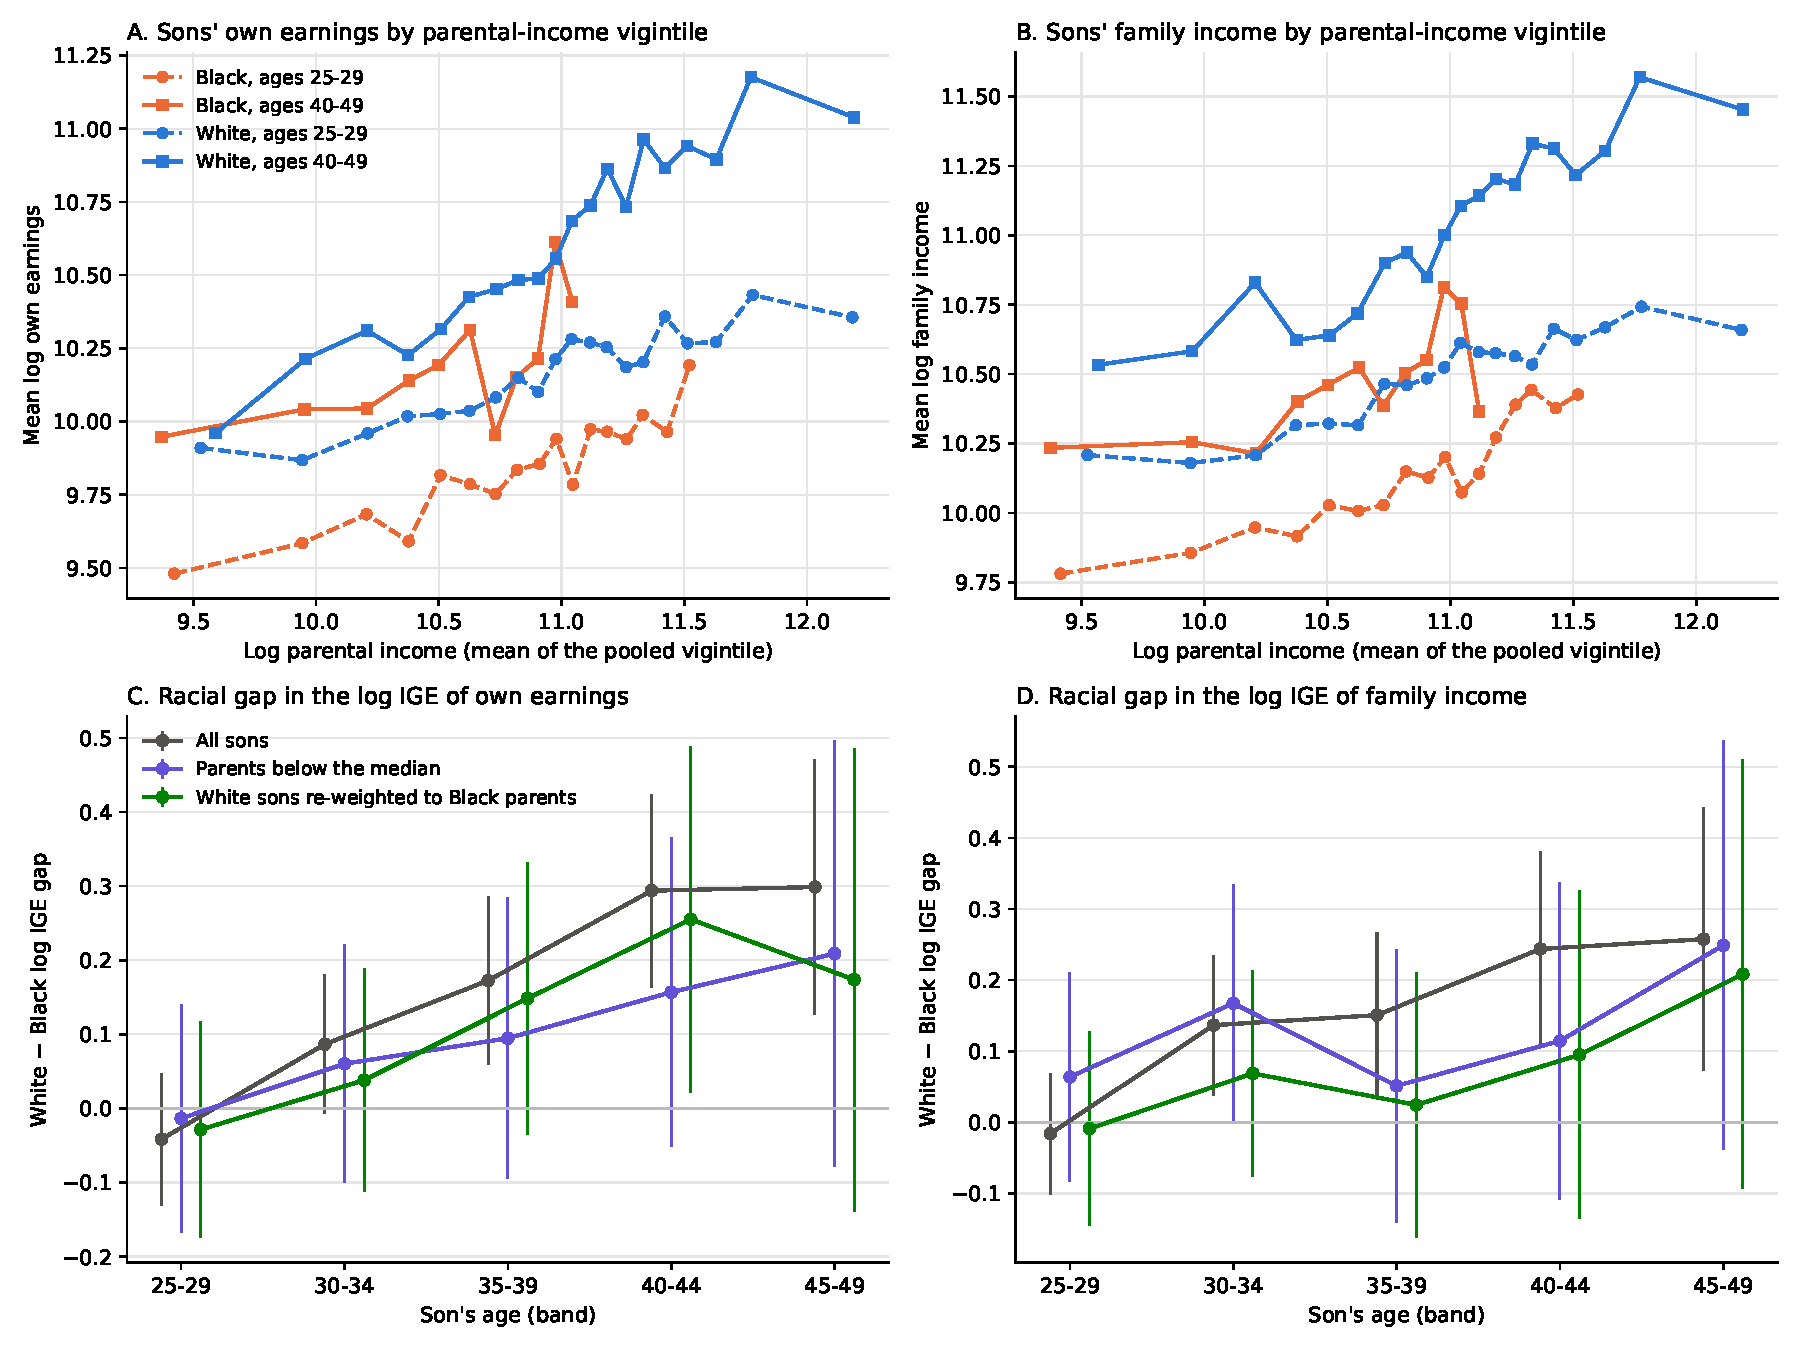
\includegraphics[width=\textwidth]{paperB_position.pdf}
\caption{Race or position in the parental distribution? (PSID, sons)}\label{fig:position}
\begin{minipage}{\textwidth}\footnotesize \textit{Notes:} Panels A and B: mean log outcome (net of race-specific
single-age means) by vigintile of the pooled parental-income distribution of Black and White sons, at 25--29 (dashed)
and 40--49 (solid); vigintiles with at least 20 sons of the race. Panels C and D: White $-$ Black gap in the log IGE by
age band, all sons, sons of parents below the pooled median, and White sons re-weighted to the Black distribution of
parental income in each band (20 bins); 95\% confidence intervals clustered by 1968 family. Code:
\texttt{41.AgeProfileMeasurement.py} and \texttt{44.PaperBReviewTables.py}.\end{minipage}
\end{figure}

\paragraph{Daughters.} Daughters' family income shows the same divergence (gap trend 0.162$^{***}$, s.e.\ 0.032),
their own earnings do not (Appendix Table~\ref{tab:ige_daughters}). The daughters' divergence runs through their
husbands (Section~\ref{sec:contains}), and it rests on the low-income oversample: on the SRC sample alone it is 0.014
(0.106).\footnote{\texttt{output/age\_profile\_robustness.md}, Section 3. Code: \texttt{33.AgeProfileRobustness.py}.}


\subsection{What opens: wages, not hours, shocks or marriage}\label{sec:contains}

Family income at a given age is the product of a household's composition, its members' hours and their wages, and it
is hit by transitory shocks. Each could produce a racial gap in persistence that opens with age. This subsection tests
them in turn. The analyses that need the father's own wage and hours use father-present sons
(Section~\ref{sec:data}); everything here is accounting, not a causal decomposition.

\paragraph{Wages, not hours.} Log earnings are the sum of the log hourly wage and log annual hours, so the elasticity of
sons' earnings with respect to fathers' earnings splits exactly into a part carried by the son's wage and a part
carried by his hours. In the age-interacted design at 40 the earnings elasticity is 0.220 for Black and 0.389 for
White sons, and the son's wage carries 0.210 and 0.378 of it, his hours 0.010 and 0.012 (Appendix
Table~\ref{tab:pricequantity}). The wage is also where the gap opens (Table~\ref{tab:wageage}). At 25--34 the elasticity
of sons' earnings with respect to fathers' earnings is 0.259 for Black and 0.258 for White sons (White $-$ Black
$-0.002$, s.e.\ 0.050), and at 35--44 it is 0.260 and 0.384 (0.123$^{*}$, s.e.\ 0.070). The gradient of the son's log
wage in parental income rises from 0.255 at 25--34 to 0.403 at 35--44 for White sons and stays at 0.161--0.163 for
Black sons, so the White $-$ Black gap in it grows from 0.094$^{***}$ to 0.240$^{***}$. The hours gradient is larger for
Black sons at 25--34 (White $-$ Black $-0.058^{***}$), so hours raise the Black elasticity and partly hide the wage gap
at young ages.\footnote{The PSID wage is annual earnings over annual hours, so the split could inherit division bias if
hours were measured with more error for Black sons; the NLSY79 hourly rate of pay gives the same direction
(Section~\ref{sec:careers}). Code: \texttt{24.IGEDecomposition.py}, Sections 1 and 1c.}

\begin{table}[!htbp]
\centering
\caption{Where the racial gap opens: wage and hours persistence by the son's age (PSID)}
\label{tab:wageage}
\resizebox{\ifdim\width>\textwidth\textwidth\else\width\fi}{!}{%
\resizebox*{!}{\ifdim\totalheight>0.85\textheight 0.85\textheight\else\totalheight\fi}{%
\begin{tabular}{lcccccc}
\toprule
Panel / group & \begin{tabular}[b]{@{}c@{}}ln family income\\on ln parental\\income\end{tabular} & \begin{tabular}[b]{@{}c@{}}ln wage\\on ln parental\\income\end{tabular} & \begin{tabular}[b]{@{}c@{}}ln hours\\on ln parental\\income\end{tabular} & \begin{tabular}[b]{@{}c@{}}ln earnings\\on father's\\ln earnings\end{tabular} & \begin{tabular}[b]{@{}c@{}}ln wage\\on father's\\ln wage\end{tabular} & \begin{tabular}[b]{@{}c@{}}ln hours\\on father's\\ln hours\end{tabular} \\
 & (1) & (2) & (3) & (4) & (5) & (6) \\
\midrule
\multicolumn{7}{l}{\textit{Sons aged 25--34}} \\
Black & $0.273^{***}$ & $0.161^{***}$ & $0.086^{***}$ & $0.259^{***}$ & $0.187^{***}$ & $0.153^{***}$ \\
 & (0.033) & (0.020) & (0.015) & (0.044) & (0.040) & (0.051) \\
White & $0.327^{***}$ & $0.255^{***}$ & $0.027^{**}$ & $0.258^{***}$ & $0.274^{***}$ & $0.131^{***}$ \\
 & (0.026) & (0.020) & (0.012) & (0.024) & (0.022) & (0.028) \\
White $-$ Black & $0.054$ & $0.094^{***}$ & $-0.058^{***}$ & $-0.002$ & $0.086^{*}$ & $-0.022$ \\
 & (0.042) & (0.028) & (0.019) & (0.050) & (0.046) & (0.058) \\
Child-years (Black / White) & 9,226 / 15,304 & 8,331 / 14,761 & 8,331 / 14,761 & 3,995 / 12,399 & 3,995 / 12,399 & 3,995 / 12,399 \\
\addlinespace
\multicolumn{7}{l}{\textit{Sons aged 35--44}} \\
Black & $0.288^{***}$ & $0.163^{***}$ & $0.059^{***}$ & $0.260^{***}$ & $0.207^{***}$ & $0.143^{***}$ \\
 & (0.046) & (0.028) & (0.017) & (0.062) & (0.054) & (0.056) \\
White & $0.474^{***}$ & $0.403^{***}$ & $0.043^{***}$ & $0.384^{***}$ & $0.393^{***}$ & $0.073^{**}$ \\
 & (0.036) & (0.031) & (0.013) & (0.033) & (0.036) & (0.031) \\
White $-$ Black & $0.186^{***}$ & $0.240^{***}$ & $-0.016$ & $0.123^{*}$ & $0.186^{***}$ & $-0.071$ \\
 & (0.058) & (0.042) & (0.022) & (0.070) & (0.065) & (0.064) \\
Child-years (Black / White) & 5,102 / 9,435 & 4,469 / 8,851 & 4,469 / 8,851 & 2,344 / 7,574 & 2,344 / 7,574 & 2,344 / 7,574 \\
\addlinespace
\multicolumn{7}{l}{\textit{Sons aged 45--55}} \\
Black & $0.250^{***}$ & $0.161^{***}$ & $0.045^{*}$ & $0.212^{**}$ & $0.162^{**}$ & $0.052$ \\
 & (0.075) & (0.045) & (0.024) & (0.089) & (0.074) & (0.073) \\
White & $0.474^{***}$ & $0.454^{***}$ & $-0.014$ & $0.403^{***}$ & $0.425^{***}$ & $0.069$ \\
 & (0.060) & (0.047) & (0.027) & (0.052) & (0.051) & (0.052) \\
White $-$ Black & $0.224^{**}$ & $0.293^{***}$ & $-0.059$ & $0.190^{*}$ & $0.262^{***}$ & $0.017$ \\
 & (0.096) & (0.065) & (0.037) & (0.103) & (0.090) & (0.090) \\
Child-years (Black / White) & 2,271 / 4,385 & 1,873 / 3,953 & 1,873 / 3,953 & 1,002 / 3,423 & 1,002 / 3,423 & 1,002 / 3,423 \\
\addlinespace
\multicolumn{7}{l}{\textit{Sons aged 25--55}} \\
Black & $0.274^{***}$ & $0.162^{***}$ & $0.072^{***}$ & $0.255^{***}$ & $0.191^{***}$ & $0.138^{***}$ \\
 & (0.036) & (0.021) & (0.013) & (0.046) & (0.043) & (0.039) \\
White & $0.391^{***}$ & $0.324^{***}$ & $0.027^{**}$ & $0.315^{***}$ & $0.332^{***}$ & $0.105^{***}$ \\
 & (0.028) & (0.022) & (0.011) & (0.025) & (0.026) & (0.027) \\
White $-$ Black & $0.117^{**}$ & $0.163^{***}$ & $-0.045^{***}$ & $0.060$ & $0.141^{***}$ & $-0.033$ \\
 & (0.046) & (0.031) & (0.017) & (0.052) & (0.050) & (0.048) \\
Child-years (Black / White) & 16,599 / 29,124 & 14,673 / 27,565 & 14,673 / 27,565 & 7,341 / 23,396 & 7,341 / 23,396 & 7,341 / 23,396 \\
\bottomrule
\end{tabular}}}
\par\smallskip
\begin{minipage}{\textwidth}\footnotesize \textit{Notes:} One regression per cell: child-years of sons in the age band of the panel, outcome and regressor in the column header, Lee--Solon controls (quartics in the parent's age at 16 and the son's age) without the age interactions, so each coefficient is the average slope in the band. Columns (1)--(3): all sons, parental family income (mean at 13--19); columns (4)--(6): father-present sons, father's childhood-window means. White $-$ Black standard error = root sum of squared standard errors (disjoint clusters). Unweighted. Standard errors clustered by 1968 family. $^{***}$ $p<0.01$, $^{**}$ $p<0.05$, $^{*}$ $p<0.1$. Source: \texttt{24.IGEDecomposition.py} (\texttt{output/ige\_decomposition.csv}); table built by \texttt{28.PaperBTables.py}.\end{minipage}
\end{table}


\paragraph{Not shocks or instability.} Thirty-seven percent of Black sons' years at 25--55, against 19 percent of White
sons', involve displacement or unemployment. Instability nonetheless does not produce the divergence. Its gradient in
parental income is the same for the two races at every age (equality across bands, $p=0.524$;
Appendix Table~\ref{tab:mechtests}); the earnings gap computed over clean years opens with age exactly as over all years
(0.196$^{***}$ against 0.193$^{***}$); and purging shock years from both generations moves the gap by 0.002 (0.042),
removing reduced-hours years as well by 0.018 (0.044).\footnote{Appendix Tables~\ref{tab:instability} and
\ref{tab:purging}; the hours share of the father's earnings variance, which a noisier father-side measure would
inflate, accounts for about 0.02 of the gap (Table~\ref{tab:decomposition}). Code: \texttt{24.IGEDecomposition.py}.}

\paragraph{Not marriage, for sons; husbands, for daughters.} For sons the family-income and earnings elasticities are
nearly the same in both races (gaps at 40 of 0.204$^{***}$ and 0.244$^{***}$), and own earnings carry the whole
family-income gap and its rise (0.221$^{***}$); being partnered rises equally with parental income for Black and White
sons after 35, and controlling for it leaves the gap unchanged (Appendix Table~\ref{tab:mechtests}). Later marriage of White
sons of richer parents holds down their family income at 25--29, which is one reason the family-income gap starts at
zero. For daughters the divergence is in family income and not in their own earnings (gaps at 40 of 0.162$^{***}$ and
0.035), and the channel is the husband: the elasticity of the husband's earnings is 0.370$^{***}$ for White and
0.171$^{***}$ for Black daughters, and the spouse term accounts for three quarters of the daughters' family-income gap
at 40 and for 0.175$^{***}$ of its rise with age (Appendix Table~\ref{tab:incomechannels}).\footnote{Exact log split of family
income into own earnings, the spouse and other income; standard errors clustered by 1968 family. Assortative mating is
strong: the elasticity of a daughter's husband's earnings, 0.362$^{***}$, exceeds that of her own, 0.301$^{***}$
\citep[as in][]{chadwick2002intergenerational}. The daughters' divergence rests on the SEO sample, as
shown above. Code: \texttt{34.IncomeVsEarningsIGE.py}.} The racial divergence that sons show in
their own wages, daughters show in their husbands'.


\paragraph{Parental income concept.} With parents' combined labor income instead of total family income as the
parental measure, the sons' earnings result holds (an opening of 0.134$^{***}$) while the family-income result weakens
to 0.051 (0.045).\footnote{\texttt{output/age\_profile\_robustness.md}, Section 3; half of the drop is the smaller
sample with parental labor income. Code: \texttt{33.AgeProfileRobustness.py}.} Transfers and other non-labor
income in the parental measure matter for the Black family-income profile.


\subsection{Careers: same-employer growth, schooling and job moves}\label{sec:careers}

Using pairs of consecutive interviews one to two years apart at which the son stayed with the same employer, I regress
the annualised growth of his log wage on parental income (Table~\ref{tab:growthladder}). For White sons at 25--34 the
gradient is 0.021$^{***}$ (0.006): a White son whose parents had twice the income sees his wage grow about 1.4 percentage
points a year faster with the same employer, on mean growth of 5.7 percent. For Black sons it is 0.003 (0.008), and the
racial difference, 0.018$^{*}$ ($p=0.062$), is less precisely estimated than its components. The White gradient is not
measurement: over two intervals it is 0.019$^{***}$ and among strict stayers whose tenure covers both income years
0.013$^{**}$.\footnote{Controlling for the wage at the interview before the pair raises it to 0.036$^{***}$, so it is not
catch-up after a low start; over whole employer spells it is 0.019$^{***}$. \texttt{output/same\_employer\_growth\_checks.md},
Section B. Code: \texttt{36.SameEmployerGrowthChecks.py}.} About half of it is sorting into steep jobs: within the
cell of the first interview of the pair it is 0.011$^{*}$ ($p=0.095$), within the cell of the later interview 0.006
($p=0.34$), and within cells the racial difference is 0.006--0.007, not significant. Controlling for the son's years of
education lowers it to 0.008 ($p=0.17$). In the NLSY79, where the employer is observed directly in the job roster, the
White gradient is 0.008$^{*}$ and the Black gradient zero, and holding the AFQT and education fixed brings the White
gradient to 0.002: the part explained runs through education (0.0046$^{***}$), not measured ability (0.0014, $p=0.31$).
The precise statement is: for White sons the gradient is precisely estimated, half sorting and half growth within jobs,
and mostly schooling; for Black sons it is a precise zero; the racial difference in growth within the same job is not
established.\footnote{Annual growth between two interviews is too noisy to settle the part that does not run through
schooling. Cumulated over ten and twenty years of a son's own wage, the PSID gradient at equal schooling is
0.073$^{***}$ and 0.135$^{***}$ for White sons and about zero for Black sons with the 13--19 mean of parental income,
and about zero with a one-year measure, in the PSID as in the NLSY79 and NLSY97. Code:
\texttt{67.LongDifferenceH4.py}, \texttt{68.LongDifferenceMeasurement.py} and \texttt{69.LongDifferenceNLSY97.py}.}

\begin{table}[!htbp]
\centering
\caption{Wage growth with the same employer at 25--34: parental income, schooling and ability}
\label{tab:growthladder}
\resizebox{\ifdim\width>\textwidth\textwidth\else\width\fi}{!}{%
\resizebox*{!}{\ifdim\totalheight>0.85\textheight 0.85\textheight\else\totalheight\fi}{%
\begin{tabular}{lcccccccccc}
\toprule
 & \begin{tabular}[b]{@{}c@{}}PSID\\baseline\end{tabular} & \begin{tabular}[b]{@{}c@{}}PSID\\cell FE,\\first interview\end{tabular} & \begin{tabular}[b]{@{}c@{}}PSID\\cell FE,\\later interview\end{tabular} & \begin{tabular}[b]{@{}c@{}}PSID\\+ education\end{tabular} & \begin{tabular}[b]{@{}c@{}}PSID\\two-interval\\growth\end{tabular} & \begin{tabular}[b]{@{}c@{}}PSID\\strict\\stayers\end{tabular} & \begin{tabular}[b]{@{}c@{}}NLSY79\\baseline\end{tabular} & \begin{tabular}[b]{@{}c@{}}NLSY79\\+ AFQT\end{tabular} & \begin{tabular}[b]{@{}c@{}}NLSY79\\+ education\end{tabular} & \begin{tabular}[b]{@{}c@{}}NLSY79\\+ AFQT\\+ education\end{tabular} \\
 & (1) & (2) & (3) & (4) & (5) & (6) & (7) & (8) & (9) & (10) \\
\midrule
\multicolumn{11}{l}{\textit{White sons}} \\
Log parental income & $0.021^{***}$ & $0.011^{*}$ & $0.006$ & $0.008$ & $0.019^{***}$ & $0.013^{**}$ & $0.008^{*}$ & $0.004$ & $0.002$ & $0.002$ \\
 & (0.006) & (0.006) & (0.007) & (0.006) & (0.005) & (0.006) & (0.005) & (0.005) & (0.005) & (0.005) \\
Years of education &  &  &  & $0.009^{***}$ &  &  &  &  & $0.004^{***}$ & $0.004^{***}$ \\
 &  &  &  & (0.002) &  &  &  &  & (0.001) & (0.001) \\
AFQT (1 s.d.) &  &  &  &  &  &  &  & $0.009^{***}$ &  & $0.003$ \\
 &  &  &  &  &  &  &  & (0.003) &  & (0.003) \\
\addlinespace
\multicolumn{11}{l}{\textit{Black sons}} \\
Log parental income & $0.003$ & $0.004$ & $-0.001$ & $0.002$ & $-0.001$ & $0.010$ & $0.000$ & $0.000$ & $-0.002$ & $-0.001$ \\
 & (0.008) & (0.010) & (0.009) & (0.008) & (0.007) & (0.008) & (0.005) & (0.005) & (0.005) & (0.005) \\
Years of education &  &  &  & $0.002$ &  &  &  &  & $0.003$ & $0.004$ \\
 &  &  &  & (0.003) &  &  &  &  & (0.002) & (0.002) \\
AFQT (1 s.d.) &  &  &  &  &  &  &  & $0.003$ &  & $-0.003$ \\
 &  &  &  &  &  &  &  & (0.005) &  & (0.005) \\
\addlinespace
\multicolumn{11}{l}{\textit{White $-$ Black}} \\
Log parental income & $0.018^{*}$ & $0.006$ & $0.007$ & $0.006$ & $0.019^{**}$ & $0.003$ & $0.009$ & $0.004$ & $0.004$ & $0.003$ \\
 & (0.010) & (0.012) & (0.011) & (0.010) & (0.008) & (0.010) & (0.007) & (0.007) & (0.007) & (0.007) \\
Years of education &  &  &  & $0.006^{*}$ &  &  &  &  & $0.001$ & $0.000$ \\
 &  &  &  & (0.003) &  &  &  &  & (0.002) & (0.003) \\
AFQT (1 s.d.) &  &  &  &  &  &  &  & $0.006$ &  & $0.006$ \\
 &  &  &  &  &  &  &  & (0.006) &  & (0.006) \\
\bottomrule
\end{tabular}}}
\par\smallskip
\begin{minipage}{\textwidth}\footnotesize \textit{Notes:} Pairs of consecutive interviews one to two years apart at which the son is with the same employer (PSID: tenure covers the interval; NLSY79: the same employer in the job roster), sons aged 25--34 at the later interview. Outcome: annualised growth of the log hourly wage. One regression per column and race; controls in every column: quartic in age, year (round) fixed effects. Cell: 11 occupation groups $\times$ 33 industry groups. Two-interval growth: the same employer at three interviews. Strict stayers: tenure covers both income years. NLSY79 columns: common sample with AFQT and education known; AFQT standardised within birth year. White $-$ Black: difference of the separate regressions, joint influence functions, clustered by 1968 family (PSID) or 1979 household (NLSY79). $^{***}$ $p<0.01$, $^{**}$ $p<0.05$, $^{*}$ $p<0.1$. Source: \texttt{IGE/36.SameEmployerGrowthChecks.py} (\texttt{output/same\_employer\_growth\_checks.csv}).\end{minipage}
\end{table}



If schooling carries the gradient, the distinctive prediction is that its pay-off grows over the career.
\citet{bhuller2017life} show in Norwegian registers that education premiums rise steeply with age.
Table~\ref{tab:schooling} estimates the return to a year of schooling in the PSID by age band and race. For White sons the
return in hourly wages rises from 0.049 at 25--29 to 0.128 at 40--44, and in earnings from 0.045 to 0.143; for Black sons
it starts higher---0.076 in wages and 0.124 in earnings at 25--29---and rises much less in wages and not at all in
earnings (0.12--0.15 at every age). The White--Black difference in the rise is 0.032$^{***}$ (0.011) in wages and
0.055$^{***}$ (0.014) in earnings, and 0.013$^{*}$ (0.008) for the NLSY79 hourly rate of pay. Education accounts for a
large part of the divergence: adding years of schooling to the regression of the log wage on parental income by band
removes 0.057$^{***}$ of the pooled rise of wage persistence after 35 (a share of 0.44$^{***}$), and 0.069$^{***}$ of the
0.186$^{***}$ change in the racial gap (0.37$^{***}$); for earnings 0.090$^{***}$ of 0.203$^{***}$ (0.44$^{***}$), and in
the NLSY79 0.038$^{***}$ of 0.054$^{**}$ (0.72$^{**}$). Education is an outcome of the same background, so these are
shares of accounting, not causal mediation.\footnote{Code: \texttt{42.SchoolingAndJobGrowth.py}
(\texttt{output/schooling\_job\_growth.md}).}


\paragraph{Within jobs, net of the calendar, holding ability fixed.} A steeper White return could reflect access alone:
if good jobs accumulate human capital faster and educated White sons get more of them, the return to schooling rises
faster with age for White sons with no racial difference in what schooling does on a given job. The test holds the job
fixed (Table~\ref{tab:withincell}). On son-years with an early job, the White--Black difference in the rise of the
earnings return is 0.058$^{***}$ (0.014) without cell controls, 0.061$^{***}$ (0.018) with fixed effects for the son's
cell at 25--34 and 0.066$^{***}$ (0.016) with fixed effects for his current cell; in wages 0.031$^{***}$, 0.029$^{*}$ and
0.036$^{***}$. Holding the early job fixed halves the rise of the earnings return in the pooled sample (from 0.050$^{***}$ to
0.025$^{***}$), so half of the rising return is the sorting of the educated into steep jobs; but it lowers the rise for
both races alike, and the racial difference does not move (changes of $-0.002$ to 0.009, s.e.\ 0.011--0.016).
The rise of the college premium over 1980--2000 could make a return rise with age that is really a rise with calendar
time; allowing the return to trend with the calendar leaves the racial difference in the rise at 0.063$^{**}$ (0.027)
for earnings and 0.035 ($p=0.12$) for wages, and within the cohorts born 1955--69 it is 0.051$^{***}$ and 0.029$^{*}$. In
the NLSY79, a single cohort, the difference is 0.017$^{*}$ within the current cell and 0.021$^{**}$ (0.009) when the AFQT
is held fixed. The Black sons' higher return at 25--29 also survives the job (0.061$^{***}$ in earnings within the early
cell) in the PSID, but not in the NLSY79 (0.008).\footnote{Code: \texttt{45.WithinCellIdentification.py}
(\texttt{output/within\_cell\_identification.md}); NLSY79 AFQT results in Appendix Table~\ref{tab:afqtgrowth}.}

The age pattern of the returns says which mechanism this is. Under employer learning the coefficient on schooling, which
employers see, falls with experience, and the coefficient on ability, which they learn, rises
\citep{altonji2001employer, lange2007speed, arcidiacono2010beyond}. In the NLSY79 both rise: with the AFQT and schooling
in the same regression, the schooling coefficient rises by 0.049$^{***}$ from the bands below 35 to the bands above, and
the AFQT coefficient by 0.036$^{***}$, and the AFQT rise does not differ by race ($-0.031$, s.e.\ 0.025). A rising return
to schooling is the complementarity of schooling with human capital accumulated on the job \citep{bhuller2017life},
and it is this complementarity that is weaker for Black sons, within the same job and at equal measured ability.
The return to experience itself does not differ by race at equal AFQT: in the within-decile regression of
\citet{rauh2023black}, run on the NLSY79 with its supplemental Black sample, hourly earnings grow with experience at the
same rate for Black and White men (Black $\times$ experience 0.003 in logs, s.e.\ 0.003, $p = 0.30$; 1,184 Black men).
Their model holds accumulation race-neutral given the AFQT and has no schooling; the racial difference here is in how
growth varies with schooling.\footnote{Hourly earnings (2018 dollars, and logs) on Black, years of accumulated
experience, their product and region fixed effects by AFQT decile, men aged 23--54 not in school, at least 500 hours and
25 weeks in the year; standard errors clustered by person. On the cross-sectional sample (285 Black men) the regression
reproduces their pattern: no difference in deciles 1--5, and negative Black $\times$ experience in deciles 9 and 10
($-1.03^{**}$ and $-1.93^{***}$ dollars a year, $p = 0.034$ and $p < 0.001$), cells that hold 4 and 3 Black men. With
the supplemental sample no decile differs and the slope pooled within deciles is 0.028 dollars a year (s.e.\ 0.071,
$p = 0.70$). Code: \texttt{70.RauhReplication.py}; output \texttt{output/rauh\_replication.md}.}
The same-employer evidence points the same way but is weaker: a year of schooling raises same-employer wage growth at
25--34 by 0.010$^{***}$ for White and 0.003 for Black sons (difference 0.007$^{**}$, $p=0.030$), and within the cell of
the first interview the difference is 0.004 ($p=0.37$); in the NLSY79 it is 0.002 ($p=0.47$) and 0.005$^{*}$ within the
cell.


Wage growth comes from staying, from moving and from losing jobs \citep{topel1992job, altonji2013modeling}.
Table~\ref{tab:jobmoves} splits the parental-income gradient of annual wage growth into these three parts. For White
sons at 25--34 the gradient of 0.020$^{***}$ is almost all within jobs: 0.017$^{***}$ comes from years with the same
employer, 0.001 from moves and 0.003 from displacements. For Black sons the within-job part is 0.005, and moves
contribute $-0.008^{**}$: Black sons of richer parents gain less, not more, when they change employers. Of the racial
difference in the growth gradient at 25--34, 0.021$^{***}$, about three fifths is within jobs (0.012$^{*}$) and two fifths
at moves (0.009$^{**}$); the racial difference in the gain at a move is 0.069$^{**}$ (0.028). Family background buys the
same protection from job loss in both races: the probability of displacement falls with parental income by 0.037$^{***}$
for White and 0.038$^{***}$ for Black sons.

\begin{table}[!htbp]
\centering
\caption{Wage growth within and between jobs by parental income (PSID, sons)}
\label{tab:jobmoves}
\resizebox{\ifdim\width>\textwidth\textwidth\else\width\fi}{!}{%
\resizebox*{!}{\ifdim\totalheight>0.85\textheight 0.85\textheight\else\totalheight\fi}{%
\begin{tabular}{lcccccccc}
\toprule
 & \begin{tabular}[b]{@{}c@{}}Wage growth,\\all pairs\end{tabular} & \begin{tabular}[b]{@{}c@{}}Contribution:\\stayed\end{tabular} & \begin{tabular}[b]{@{}c@{}}Contribution:\\moved\end{tabular} & \begin{tabular}[b]{@{}c@{}}Contribution:\\displaced\end{tabular} & \begin{tabular}[b]{@{}c@{}}Stayed\end{tabular} & \begin{tabular}[b]{@{}c@{}}Displaced\end{tabular} & \begin{tabular}[b]{@{}c@{}}Growth\\if stayed\end{tabular} & \begin{tabular}[b]{@{}c@{}}Growth\\if moved\end{tabular} \\
 & (1) & (2) & (3) & (4) & (5) & (6) & (7) & (8) \\
\midrule
\multicolumn{9}{l}{\textit{Sons aged 25--34}} \\
White: log parental income & $0.020^{***}$ & $0.017^{***}$ & $0.001$ & $0.003$ & $0.035^{***}$ & $-0.037^{***}$ & $0.020^{***}$ & $0.005$ \\
 & (0.005) & (0.004) & (0.002) & (0.002) & (0.012) & (0.009) & (0.006) & (0.017) \\
Black: log parental income & $-0.001$ & $0.005$ & $-0.008^{**}$ & $0.002$ & $0.035^{**}$ & $-0.038^{***}$ & $0.004$ & $-0.064^{***}$ \\
 & (0.006) & (0.005) & (0.003) & (0.004) & (0.016) & (0.014) & (0.008) & (0.023) \\
White $-$ Black: log parental income & $0.021^{***}$ & $0.012^{*}$ & $0.009^{**}$ & $0.000$ & $0.000$ & $0.001$ & $0.016$ & $0.069^{**}$ \\
 & (0.008) & (0.007) & (0.004) & (0.005) & (0.020) & (0.017) & (0.010) & (0.028) \\
\addlinespace
\multicolumn{9}{l}{\textit{Sons aged 35--55}} \\
White: log parental income & $0.007^{**}$ & $0.003$ & $0.004^{**}$ & $0.000$ & $0.033^{***}$ & $-0.021^{**}$ & $0.003$ & $0.046^{***}$ \\
 & (0.003) & (0.003) & (0.002) & (0.001) & (0.011) & (0.008) & (0.004) & (0.017) \\
Black: log parental income & $-0.002$ & $0.000$ & $-0.002$ & $-0.001$ & $-0.005$ & $0.000$ & $0.000$ & $-0.013$ \\
 & (0.004) & (0.003) & (0.002) & (0.003) & (0.015) & (0.011) & (0.004) & (0.020) \\
White $-$ Black: log parental income & $0.009^{*}$ & $0.003$ & $0.006^{**}$ & $0.000$ & $0.039^{**}$ & $-0.021$ & $0.002$ & $0.059^{**}$ \\
 & (0.005) & (0.004) & (0.003) & (0.003) & (0.019) & (0.014) & (0.005) & (0.026) \\
\bottomrule
\end{tabular}}}
\par\smallskip
\begin{minipage}{\textwidth}\footnotesize \textit{Notes:} Consecutive interviews one to two years apart with a valid wage, a mapped occupation and tenure (waves 1985--2023). Between the two wage years the son stayed with the employer, moved without displacement, or was displaced (plant closure, layoff or firing). Columns (2)--(4) are the wage growth times an indicator of the event and add up to column (1) on the same pairs (column (3) and (4) of the moved and displaced contributions); (5)--(6) linear probabilities; (7)--(8) growth conditional on the event. Each cell: coefficient on log parental income; controls: quartic in age, year fixed effects; standard errors clustered by 1968 family. $^{***}$ $p<0.01$, $^{**}$ $p<0.05$, $^{*}$ $p<0.1$. Source: \texttt{IGE/42.SchoolingAndJobGrowth.py} (\texttt{output/schooling\_job\_growth.csv}).\end{minipage}
\end{table}


\subsection{What does not carry the divergence}

Entry into supervisory and managerial occupations, the closest observable analogue to the promotion delays documented
by \citet{hegde2026racial}, rises with parental income after 35 for White and not for Black sons (a racial difference of
0.024$^{***}$ at 35--55), but the change of that difference relative to 25--34 is 0.008 (0.011), and self-reported
position changes and promotions show no Black deficit. Job loss is frequent and costly---displacement lowers the son's log
wage two to three years later by 0.131$^{***}$, of which 0.028$^{***}$ is a lower occupational score---but the
occupational loss is not larger for Black sons, and shocks do not account for the divergence (Section~\ref{sec:contains}).
These results, the industry decompositions and the NLSY79 replication of the occupational split are in
Appendix~\ref{app:careers}.


\subsection{Fathers' jobs}\label{sec:fathers}

Parents' employers and networks shape where young people find their first job and raise their initial earnings
\citep{corak2011intergenerational, kramarz2014strong, staiger2022}. The PSID does not identify employers, and neither
do the public NLSY files for fathers, so working for the father's employer cannot be observed; the father's occupation
group and his occupation-by-industry cell, his modal codes when the son was 12--18, are the proxies.\footnote{The
father is the male head of the son's family at 16, so these measures exist for 52 percent of Black and 87 percent of
White sons. Fathers are coded in 1970 Census codes and sons after 2001 in 2000 or 2010 codes; the 35--55 window falls
more often after 2001, so coding drift lowers measured following after 35, which works against the convergence below.
Code: \texttt{32.IndustryCareers.py}, \texttt{35.EarlyIndustryLatePayoff.py} and
\texttt{43.FatherJobSelfEmployment.py}.}

\paragraph{Following pays at entry, not in growth.} Sons work in their father's industry group two to three times as
often as random matching within race and parental-income tercile would predict (14.2 percent of White sons at 35--55
against a benchmark of 5.1 percent, and 10.1 percent of Black sons against 5.4 percent). Holding the son's education
and the level and slope of his industry fixed, sons in their father's industry group earn 0.079$^{***}$ more at 25--34
and 0.054$^{*}$ more at 35--55, but their wages grow no faster (0.005, s.e.\ 0.005), and following accounts for none of
the racial divergence ($-0.002$ of 0.107$^{**}$).\footnote{Appendix Table~\ref{tab:fatherindustry} and
\texttt{output/industry\_careers.md}, Section 4. Few Black fathers worked in high-paying service industries (21 in
finance, insurance or real estate), so industry-specific following cannot be estimated for Black sons.} Family networks,
as measured here, transmit a starting advantage that is the same at every age at which the IGE is measured.

\paragraph{Convergence on the father's occupation.} Over the career, sons of richer parents converge on their fathers'
occupations (Table~\ref{tab:fatherse}). The parental-income gradient of being in the father's occupation group is
0.051$^{***}$ at 25--34 and 0.099$^{***}$ at 35--55 (change 0.052$^{***}$). The change is precisely estimated for White
sons (0.060$^{***}$) and imprecise for Black sons (0.036, s.e.\ 0.028); the two cannot be distinguished. The level of
following differs by race at every age: at 35--55, 22.4 percent of White and 15.3 percent of Black sons work in their
father's occupation group. Within the top parental tercile, sons of White parents are 11.7 percentage points more likely
than sons of Black parents to work in their father's occupation group (0.117$^{***}$, resting on 121 Black sons in that
tercile), while rich and poor White sons do not differ ($-0.086$, s.e.\ 0.061): the contrast is a racial gap in
following the father's occupation at equal parental income, not class amplifying it.

\paragraph{The father's exact job is a family business.} Whether a son holds his father's exact job---his occupation
group in his industry group---does not depend on parental income at 25--34 (0.004) and does at 35--55 (0.031$^{**}$;
change 0.023$^{**}$), because sons of richer parents who hold it in their early thirties keep it: among the 137 sons in
the father's cell at 25--34, 84 are still in it at 35--55 and 53 leave, and leaving falls with parental income
($-0.206^{***}$); entry after 34 is rare (39 of 1,892 sons) and unrelated to parental income. Only 9 of the 84 who keep
the father's job are Black. The self-employment split shows what the exact job is. Twenty-one percent of White and 8
percent of Black sons have a self-employed father, and the convergence comes entirely from them: among sons of
self-employed fathers the gradient rises by 0.065$^{***}$ after 35, among other sons by 0.009 (0.011), and among sons
for whom neither father nor son is self-employed by 0.005. The cells most often inherited after 35 are farming in
agriculture (31 sons, 56 percent of them self-employed and 75 percent with a self-employed father), craft work in
construction and management in construction. Convergence on the father's exact job is the inheritance of a farm or a
firm \citep[the business and wealth transmission of][]{fagereng2021wealthy}, not of a position in a network. The
occupation-level result is not: excluding self-employed fathers, the gradient still rises after 35 (0.037$^{*}$) and the
rich-White-versus-rich-Black contrast is unchanged (0.117$^{***}$). Keeping the father's job also does not depend on
self-employment ($-0.183^{**}$ among the 90 sons of fathers who were not self-employed), and holding the father's exact
job brings no wage premium at 35--55 and no faster wage growth.

\begin{table}[!htbp]
\centering
\caption{Fathers' jobs and self-employment (PSID, sons)}
\label{tab:fatherse}
\resizebox{\ifdim\width>\textwidth\textwidth\else\width\fi}{!}{%
\resizebox*{!}{\ifdim\totalheight>0.85\textheight 0.85\textheight\else\totalheight\fi}{%
\begin{tabular}{lcccc}
\toprule
 & \begin{tabular}[b]{@{}c@{}}All sons\end{tabular} & \begin{tabular}[b]{@{}c@{}}Father not\\self-employed\end{tabular} & \begin{tabular}[b]{@{}c@{}}Father\\self-employed\end{tabular} & \begin{tabular}[b]{@{}c@{}}Neither father\\nor son\\self-employed\end{tabular} \\
 & (1) & (2) & (3) & (4) \\
\midrule
\multicolumn{5}{l}{\textit{Son in the father's occupation $\times$ industry cell}} \\
All: log parental income, 25--34 & $0.004$ & $-0.006$ & $0.009$ & $-0.005$ \\
 & (0.012) & (0.012) & (0.023) & (0.013) \\
All: log parental income, 35--55 & $0.031^{**}$ & $0.009$ & $0.072^{***}$ & $0.008$ \\
 & (0.016) & (0.016) & (0.025) & (0.018) \\
All: log parental income $\times$ (age $\geq$ 35) & $0.023^{**}$ & $0.009$ & $0.065^{***}$ & $0.005$ \\
 & (0.010) & (0.011) & (0.021) & (0.012) \\
White: log parental income, 25--34 & $-0.005$ & $-0.011$ & $-0.005$ & $-0.007$ \\
 & (0.014) & (0.014) & (0.025) & (0.015) \\
White: log parental income, 35--55 & $0.025$ & $0.006$ & $0.065^{**}$ & $0.006$ \\
 & (0.020) & (0.020) & (0.025) & (0.023) \\
White: log parental income $\times$ (age $\geq$ 35) & $0.026^{**}$ & $0.009$ & $0.073^{***}$ & $0.004$ \\
 & (0.012) & (0.012) & (0.022) & (0.015) \\
Son-years / sons at 35--55 & 13,835 / 2,166 & 10,539 / 1,683 & 2,399 / 373 & 9,324 / 1,579 \\
\addlinespace
\multicolumn{5}{l}{\textit{Son in the father's occupation group}} \\
All: log parental income, 25--34 & $0.051^{***}$ & $0.040^{**}$ & $0.067^{**}$ & $0.037^{*}$ \\
 & (0.016) & (0.019) & (0.030) & (0.019) \\
All: log parental income, 35--55 & $0.099^{***}$ & $0.071^{***}$ & $0.163^{***}$ & $0.072^{***}$ \\
 & (0.020) & (0.026) & (0.027) & (0.027) \\
All: log parental income $\times$ (age $\geq$ 35) & $0.052^{***}$ & $0.037^{*}$ & $0.104^{***}$ & $0.038^{*}$ \\
 & (0.016) & (0.021) & (0.026) & (0.022) \\
White: log parental income, 25--34 & $0.040^{**}$ & $0.035$ & $0.042$ & $0.033$ \\
 & (0.018) & (0.022) & (0.032) & (0.022) \\
White: log parental income, 35--55 & $0.099^{***}$ & $0.073^{**}$ & $0.161^{***}$ & $0.076^{**}$ \\
 & (0.023) & (0.029) & (0.027) & (0.029) \\
White: log parental income $\times$ (age $\geq$ 35) & $0.060^{***}$ & $0.039^{*}$ & $0.124^{***}$ & $0.041^{*}$ \\
 & (0.017) & (0.022) & (0.028) & (0.024) \\
Son-years / sons at 35--55 & 13,908 / 2,174 & 10,604 / 1,691 & 2,404 / 373 & 9,383 / 1,588 \\
\addlinespace
\multicolumn{5}{l}{\textit{Race, class and keeping the father's job}} \\
Rich White $-$ rich Black, father's occupation group, 35--55 & $0.117^{***}$ & $0.117^{***}$ & $-0.019$ & $0.113^{***}$ \\
 & (0.038) & (0.040) & (0.143) & (0.043) \\
Rich White $-$ rich Black, father's cell, 35--55 & $0.011$ & $-0.008$ & $0.131^{***}$ & $-0.004$ \\
 & (0.029) & (0.030) & (0.033) & (0.033) \\
Black sons in the top tercile & 121 & 112 & 9 & 105 \\
Leaving the father's cell (in at 25--34) on log parental income & $-0.206^{***}$ & $-0.183^{**}$ & $-0.223^{*}$ & $-0.163^{**}$ \\
 & (0.066) & (0.080) & (0.126) & (0.079) \\
Sons in the father's cell at 25--34 & 137 & 90 & 46 & 82 \\
\bottomrule
\end{tabular}}}
\par\smallskip
\begin{minipage}{\textwidth}\footnotesize \textit{Notes:} Son-year linear probability models, Lee--Solon controls (quartics in the parent's age and the son's age), clusters 1968 family; all sons weighted, White sons unweighted. The father's cell is his modal 11 occupation groups $\times$ 33 industry groups when the son is 12--18; the father is self-employed when at least half of his valid interviews from 1976 on, with the son aged 10--25, report working for himself (alone or also for someone else). The change row is from one regression on 25--55 with log parental income $\times$ (age $\geq$ 35). Rich White $-$ rich Black: sons in the top pooled tercile of parental income, race $\times$ tercile cells with log parental income, weighted. Leaving: sons in the father's cell in their modal 25--34 job, out of it in their modal 35--55 job, on log parental income and a quadratic in birth cohort. These estimates use sons with a father's self-employment code (and, for leaving, a cohort quadratic and no weights); on all sons with a father's cell the same contrasts are 0.131$^{***}$ (0.038) for rich White $-$ rich Black and $-0.167^{**}$ (0.067) for leaving (	exttt{35.EarlyIndustryLatePayoff.py}, Section F). $^{***}$ $p<0.01$, $^{**}$ $p<0.05$, $^{*}$ $p<0.1$. Source: \texttt{43.FatherJobSelfEmployment.py} (\texttt{output/father\_job\_selfemp.csv}).\end{minipage}
\end{table}


The fathers' evidence adds two channels to the career evidence: a level advantage at entry through family networks,
which accounts for $-0.002$ (0.004) of the 0.107$^{**}$ change in the racial gap in wage persistence on the father-present
sample, and the inheritance of family businesses, a matter of assets rather than access, which accounts for $-0.004$ of a
0.120$^{**}$ change. Convergence on fathers' occupations outside the family firm, with its racial gap at equal parental
income, is a third. None of them carries the growth of wages that produces the divergence; that is the job at 25--34,
its access, and schooling.


\end{document}
